% !TEX root = ../thesis.tex

\chapter{Additional Plots}
\label{chap:appendixAnalysis}

\section{Control Plots}

\subsubsection{Control Plots in the Jet Mass Sideband Region}

\begin{figure}[htbp]
  \centering
  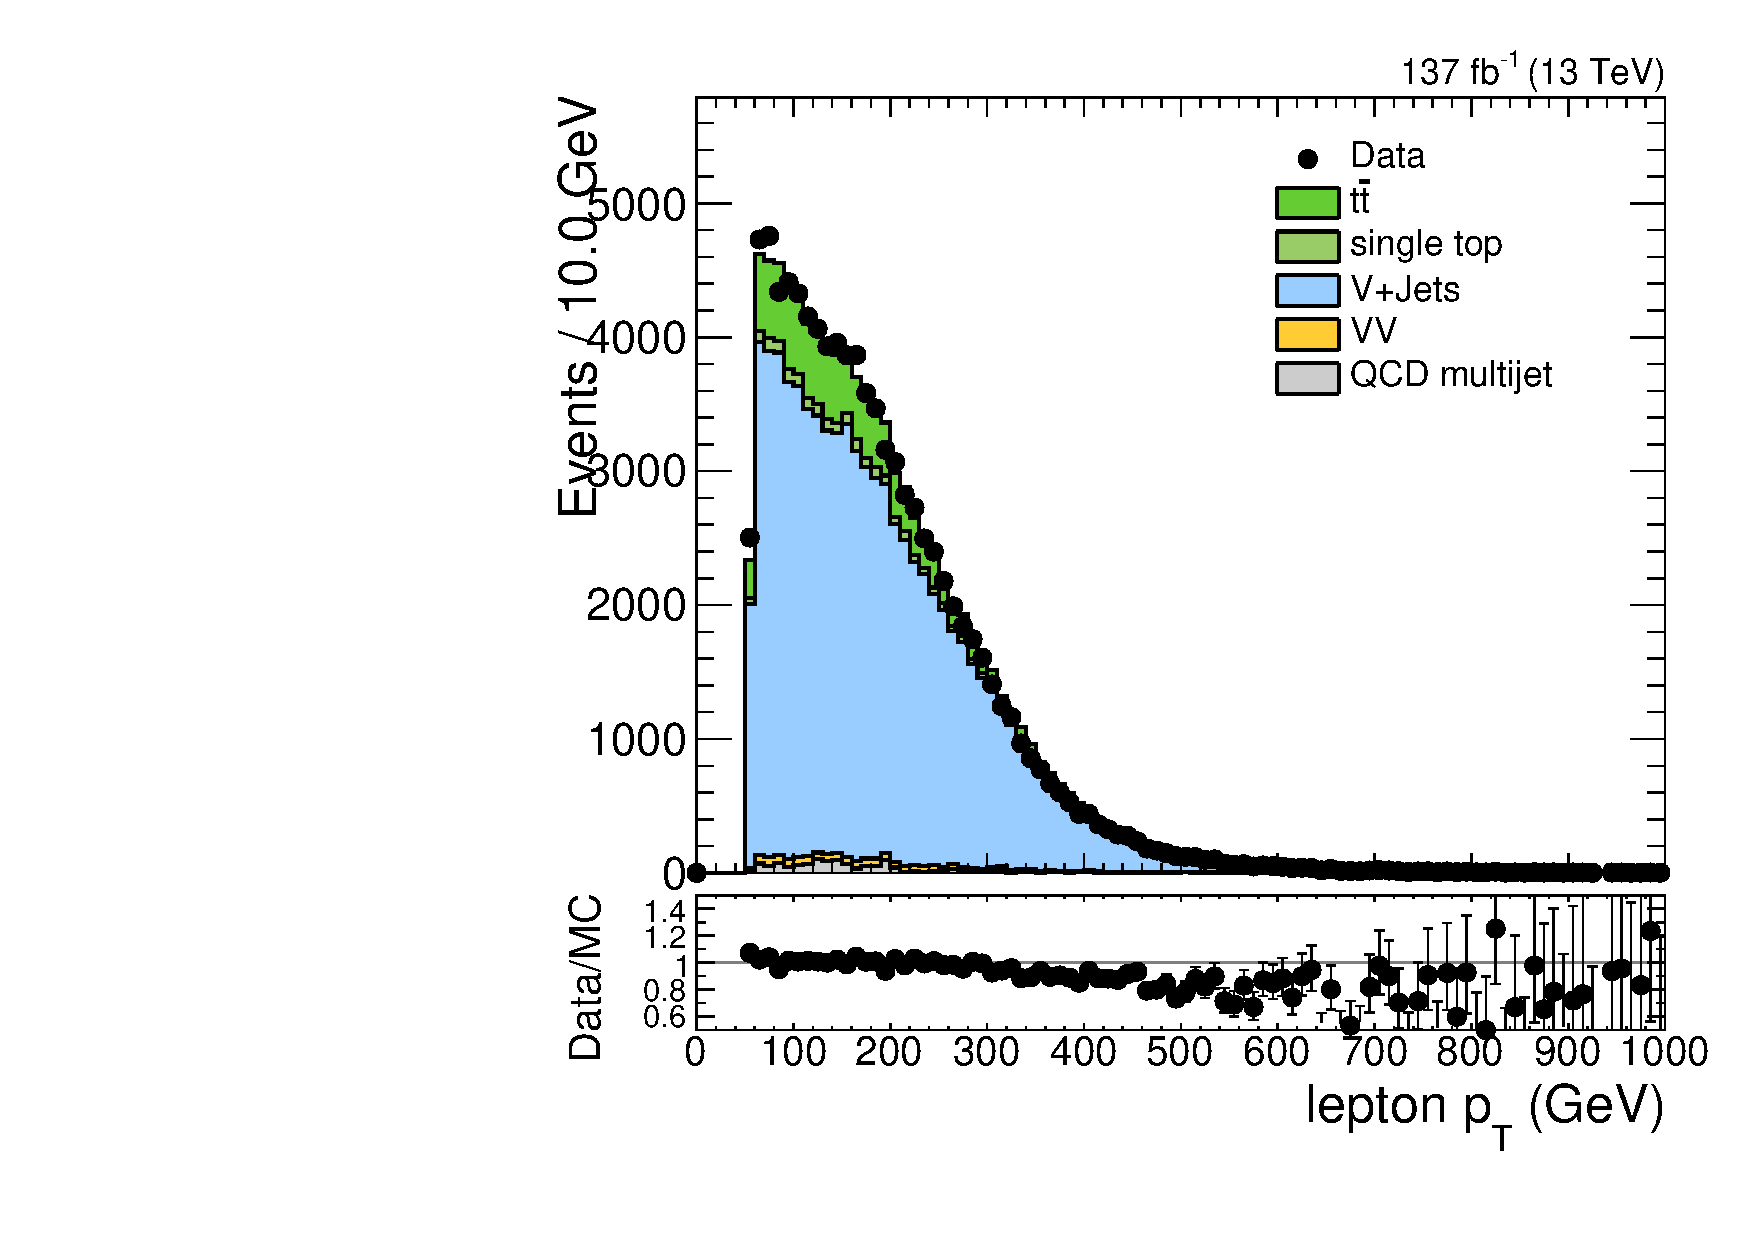
\includegraphics[width=0.3825\textwidth]{fig/analysisAppendix/SB_b1_mu_allP_allC_allD_Run2_lnujj_l1_l_pt.pdf}
  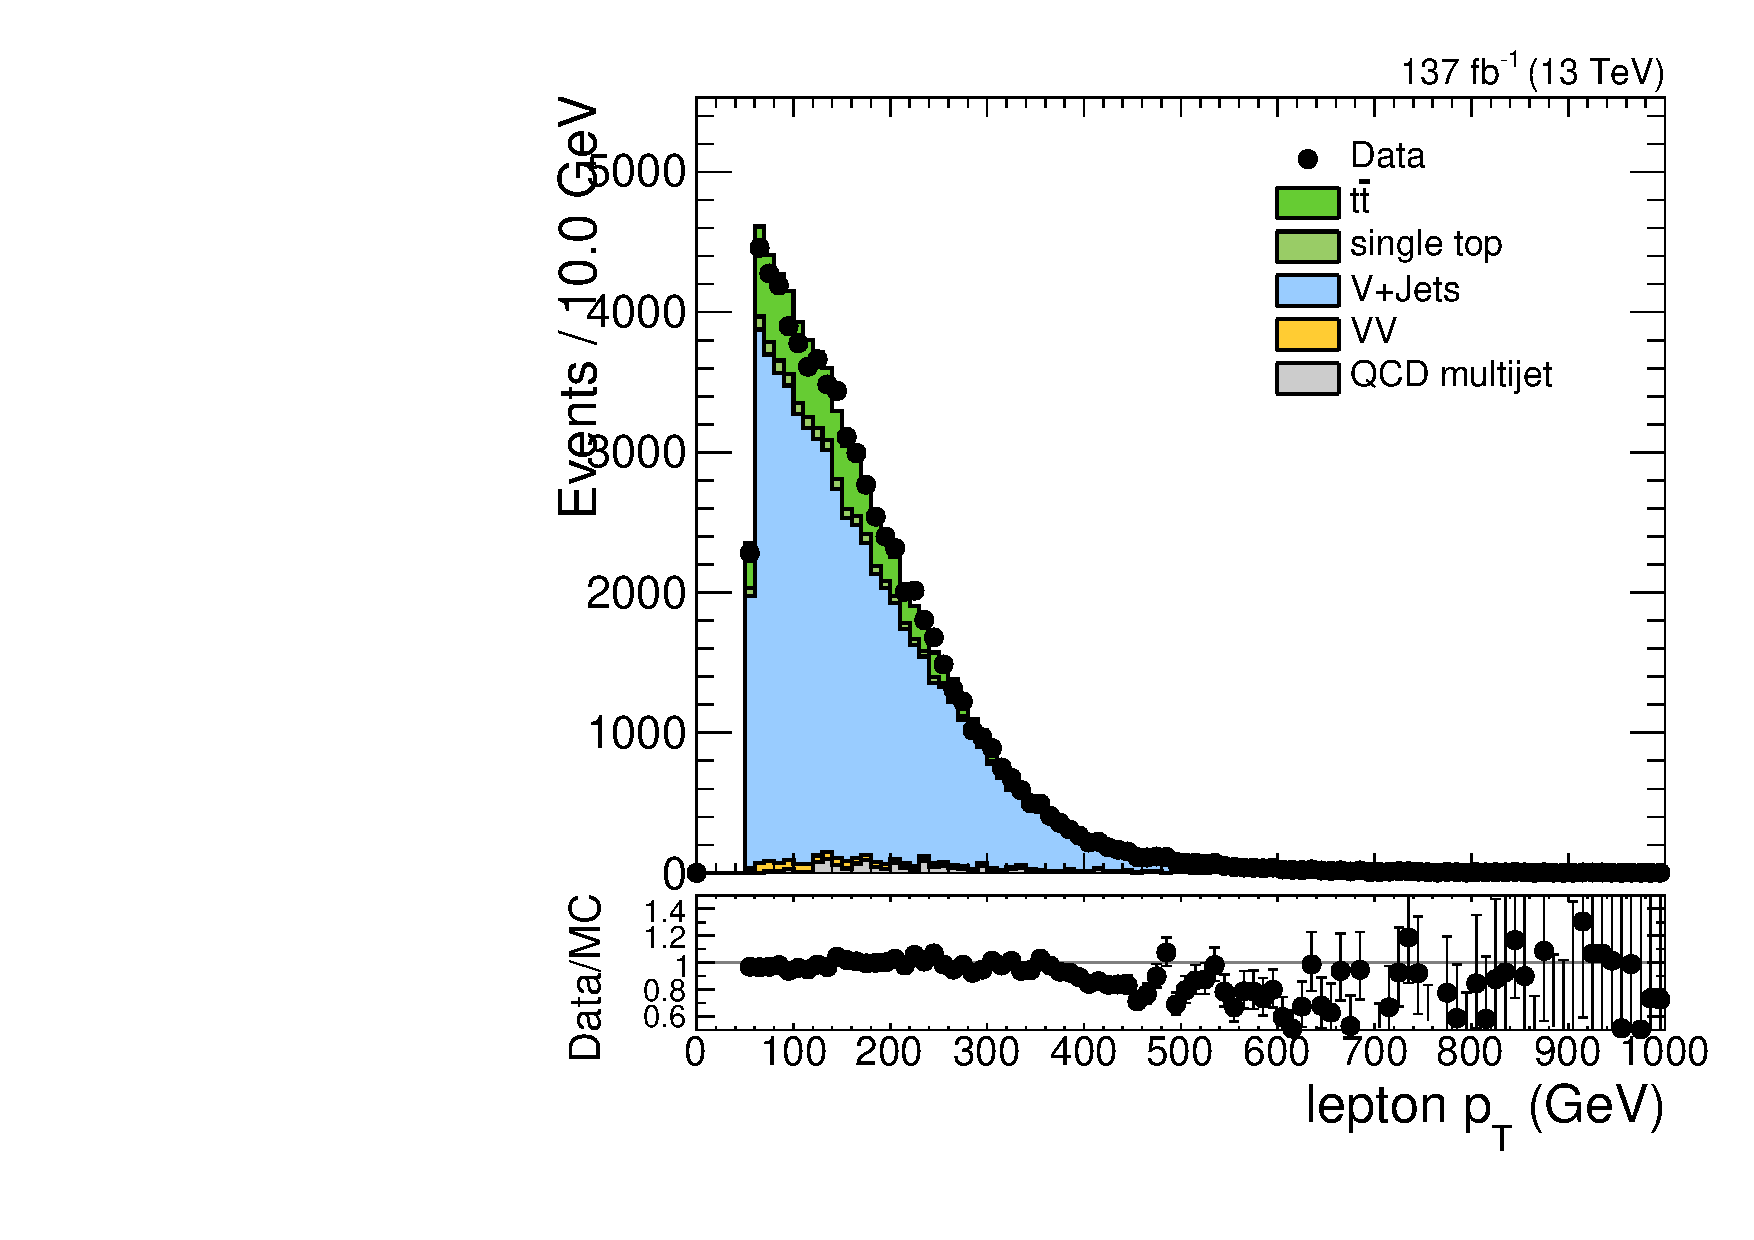
\includegraphics[width=0.3825\textwidth]{fig/analysisAppendix/SB_b1_e_allP_allC_allD_Run2_lnujj_l1_l_pt.pdf}\\
  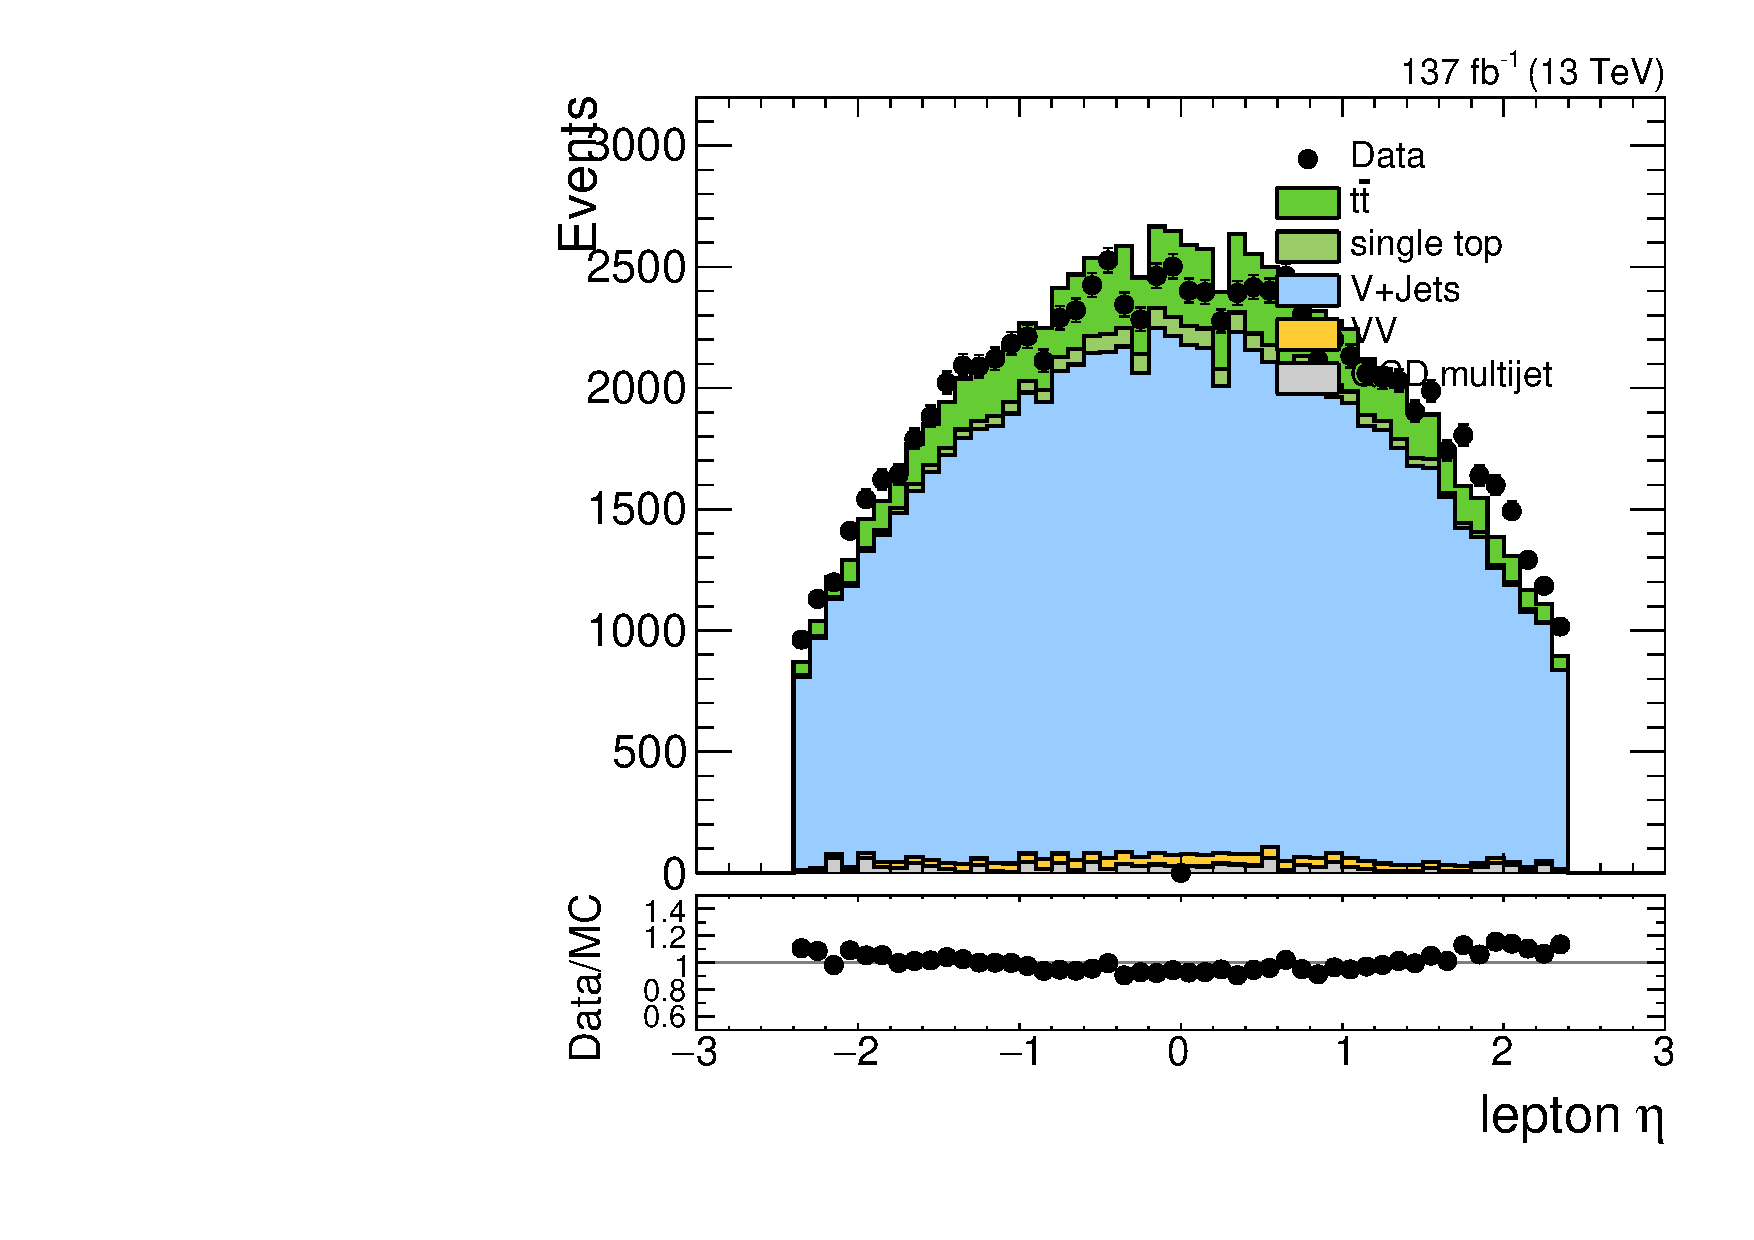
\includegraphics[width=0.3825\textwidth]{fig/analysisAppendix/SB_b1_mu_allP_allC_allD_Run2_lnujj_l1_l_eta.pdf}
  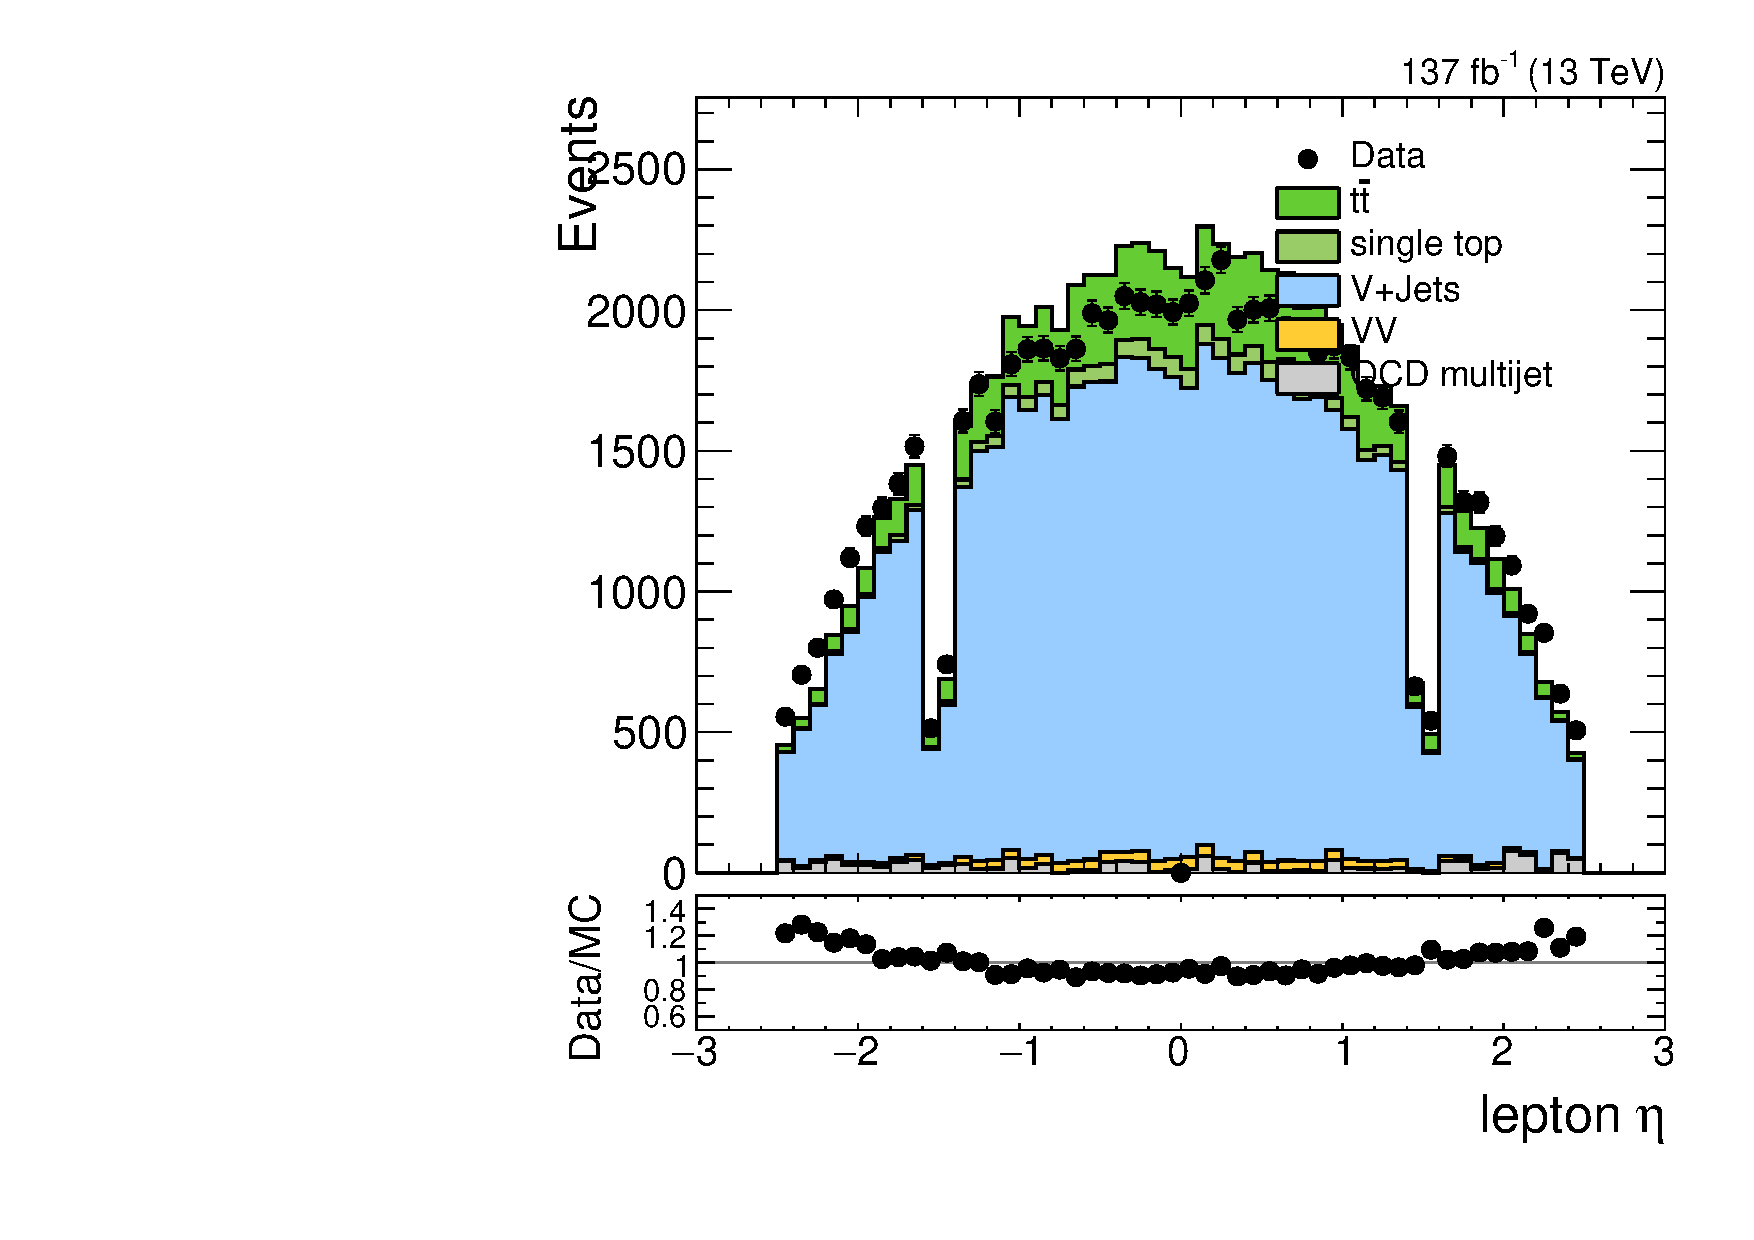
\includegraphics[width=0.3825\textwidth]{fig/analysisAppendix/SB_b1_e_allP_allC_allD_Run2_lnujj_l1_l_eta.pdf}\\
  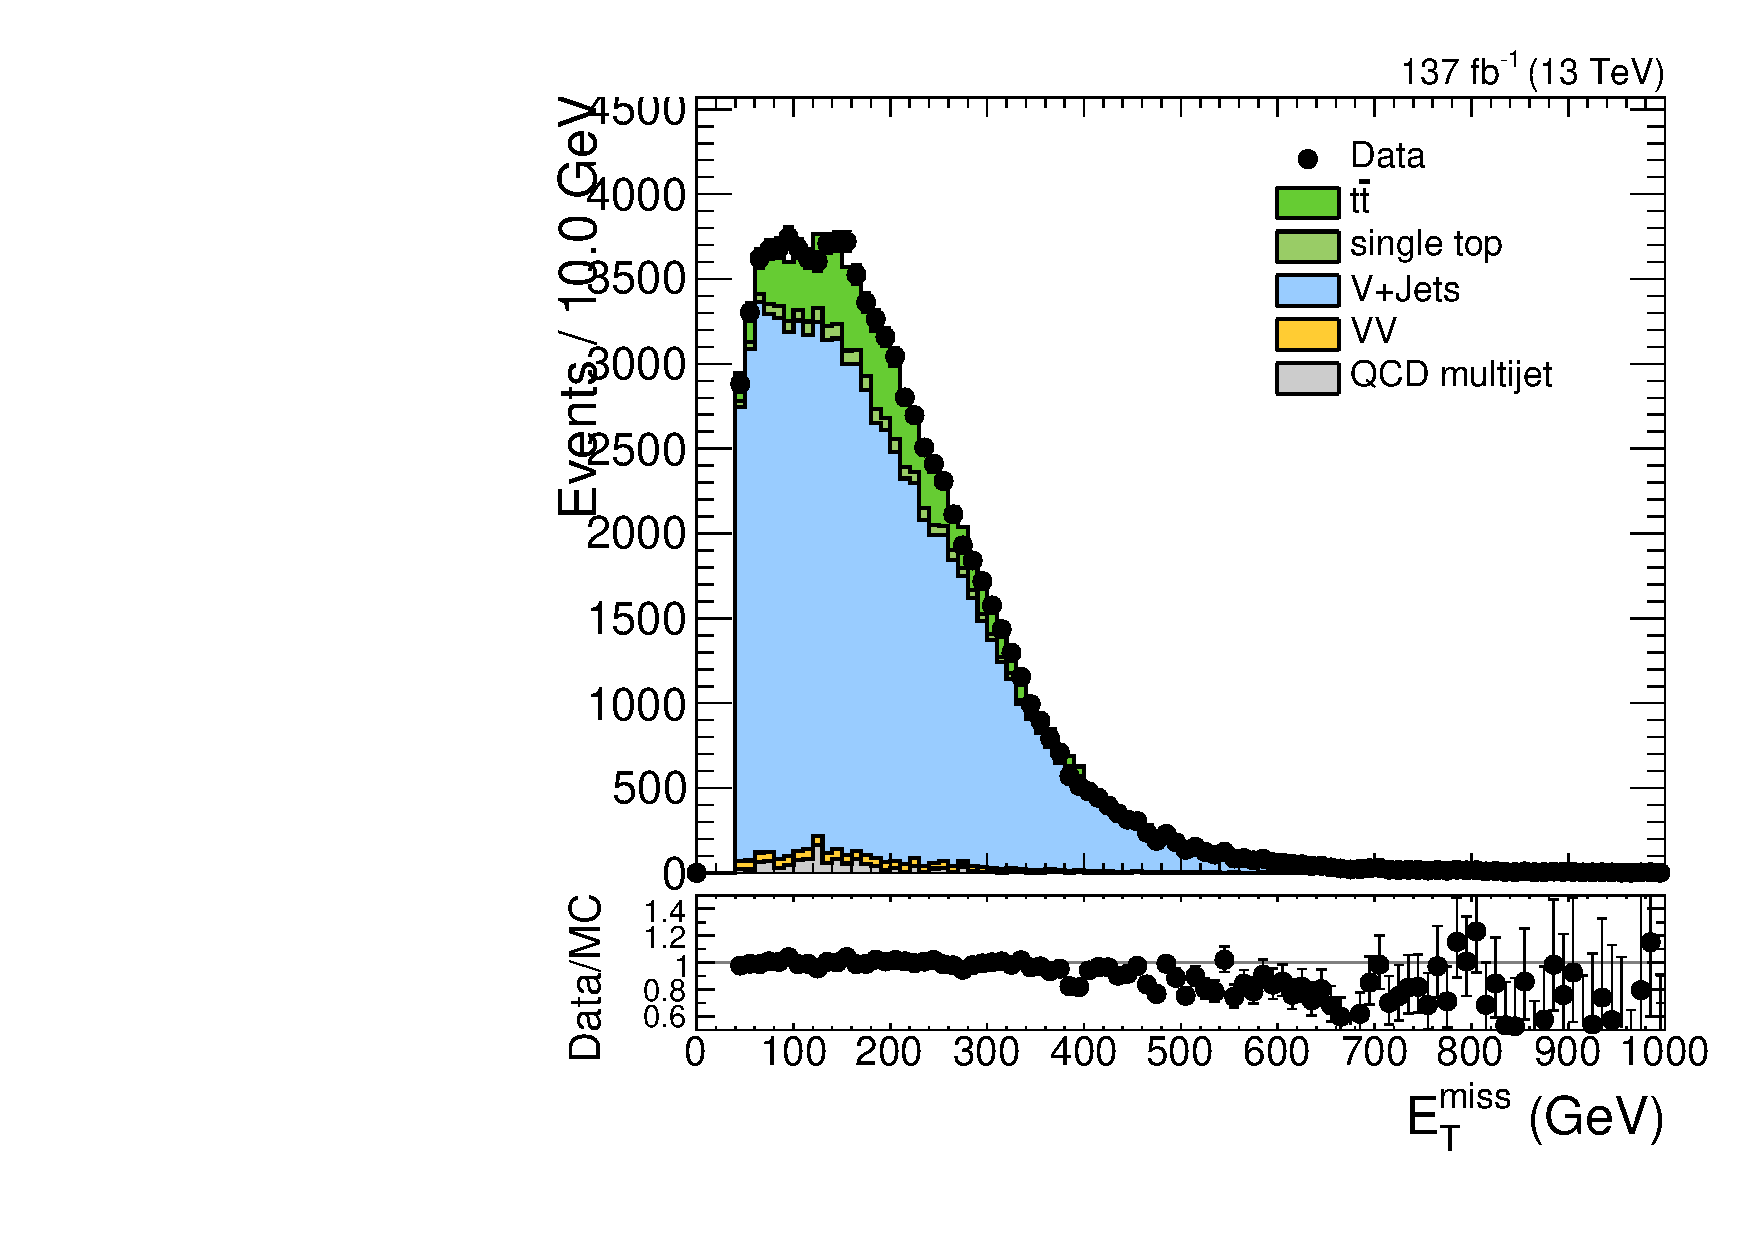
\includegraphics[width=0.3825\textwidth]{fig/analysisAppendix/SB_b1_mu_allP_allC_allD_Run2_met_pt.pdf}
  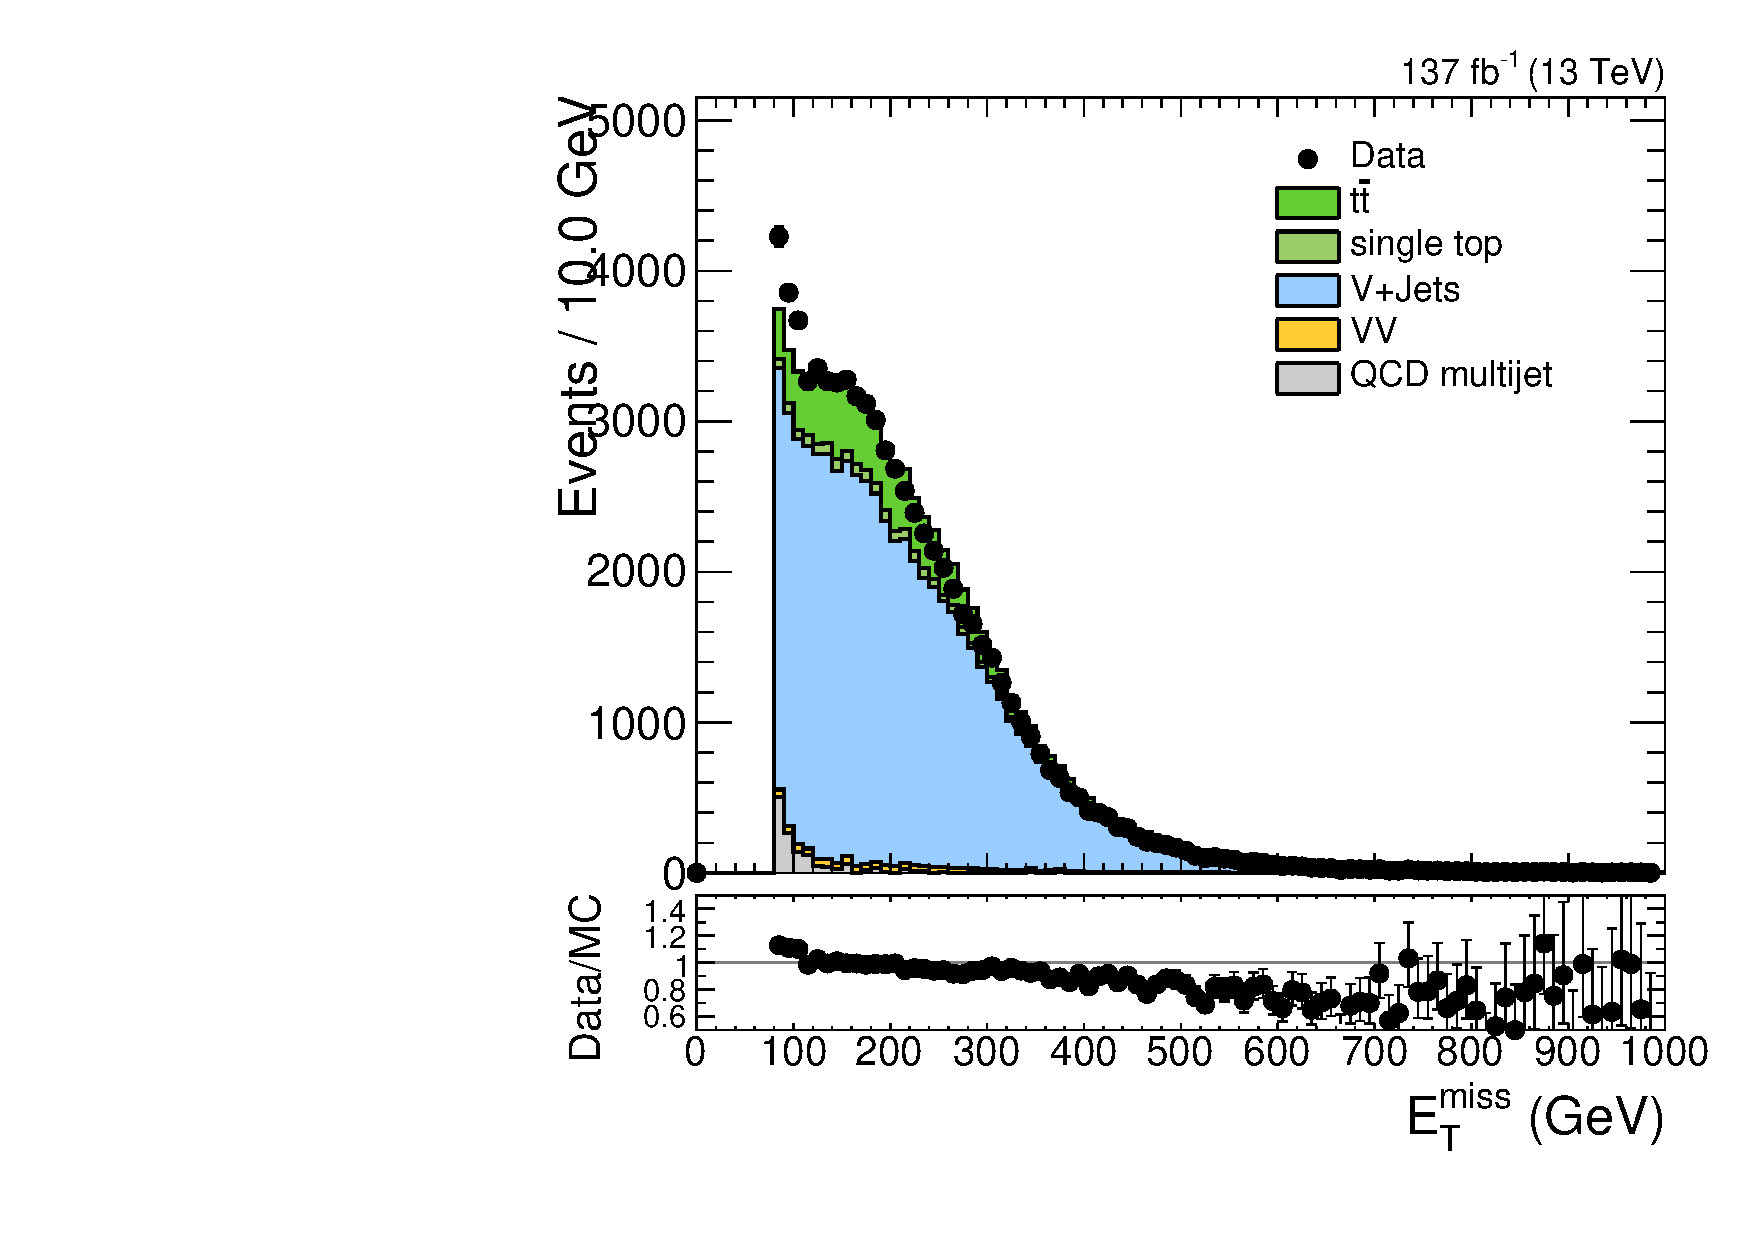
\includegraphics[width=0.3825\textwidth]{fig/analysisAppendix/SB_b1_e_allP_allC_allD_Run2_met_pt.pdf}\\
  \caption{
    Comparison plots between data and MC from Run 2 for different \Wlep-related observables, in the jet mass sideband.
    From top to bottom: lepton \pt, lepton $\eta$, \ptmiss.
    Left: muon channel, right: electron channel.
  }
  \label{fig:SB_controlPlotsRun2_1}
\end{figure}

\begin{figure}[htbp]
  \centering
  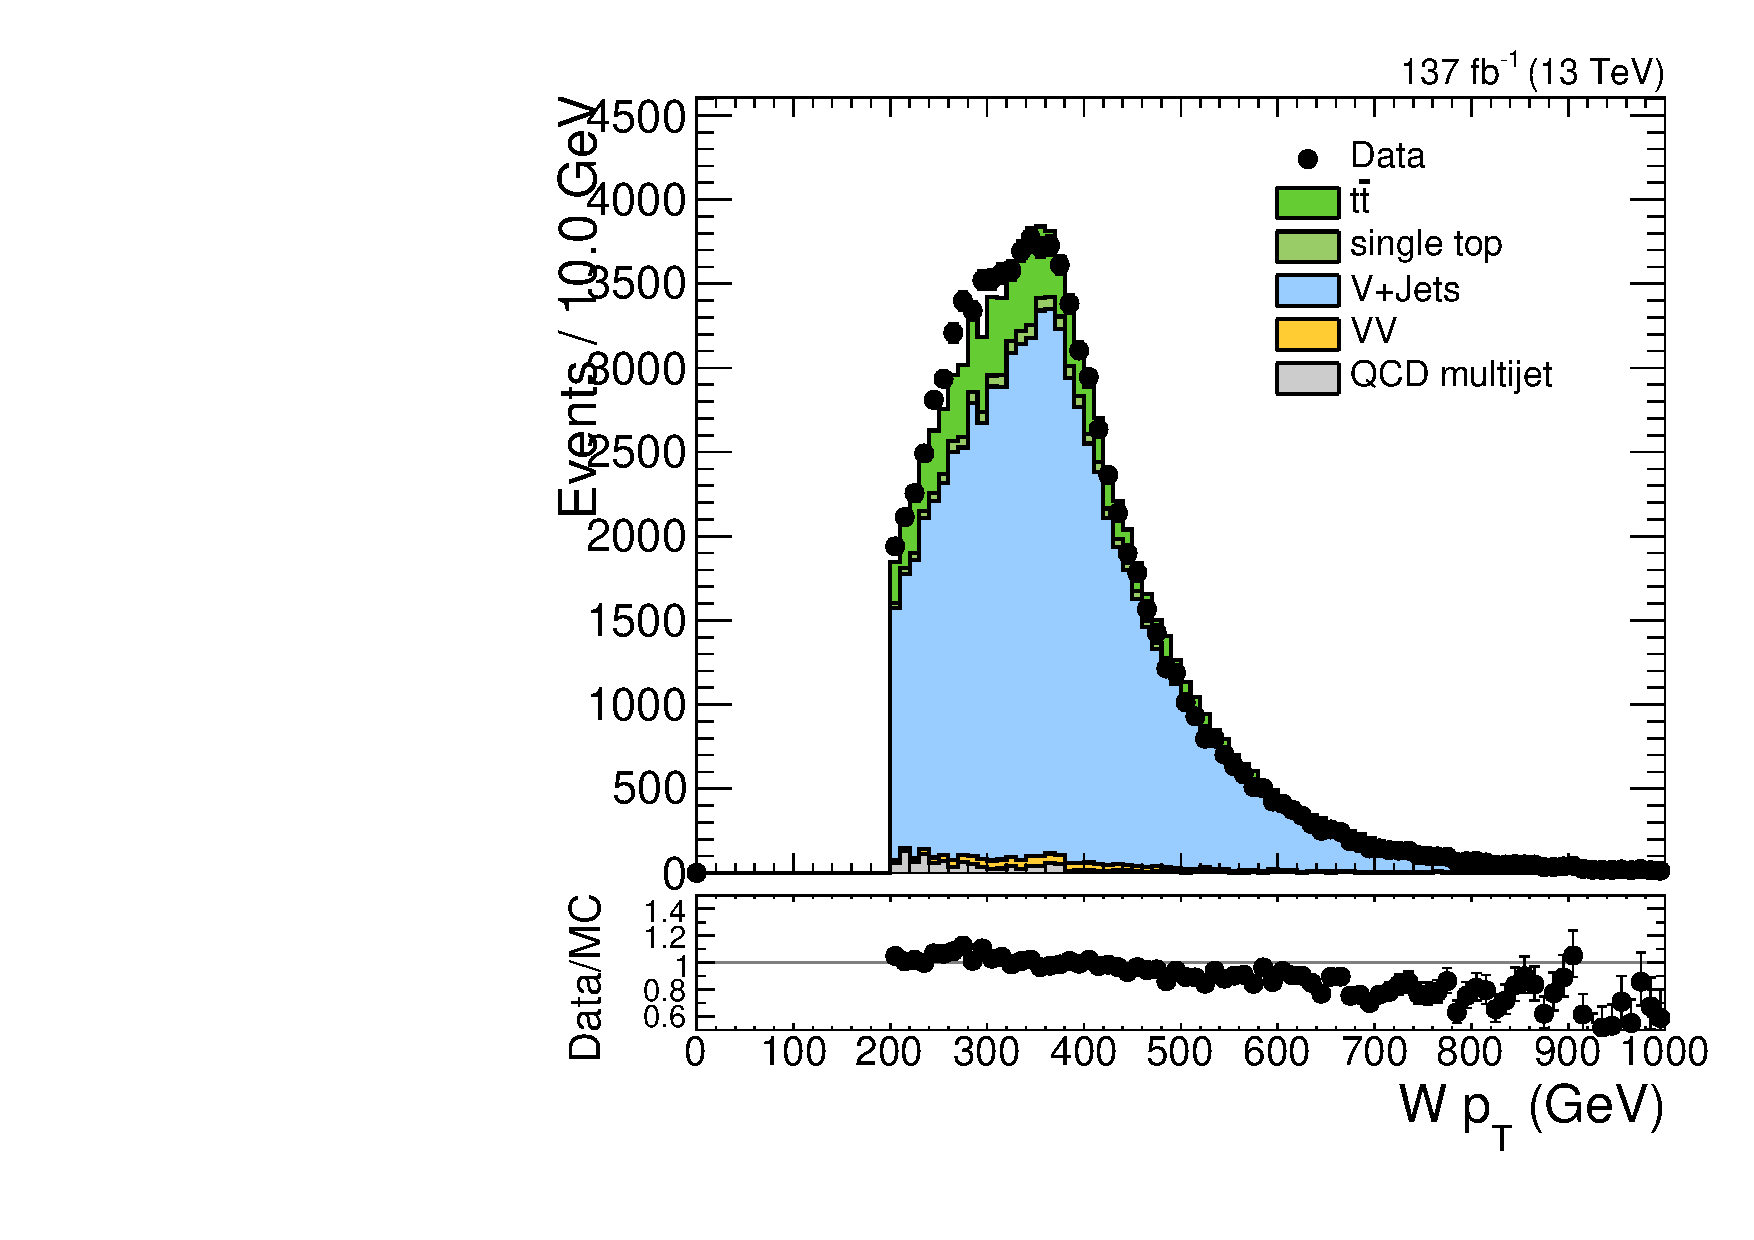
\includegraphics[width=0.3825\textwidth]{fig/analysisAppendix/SB_b1_mu_allP_allC_allD_Run2_lnujj_l1_pt.pdf}
  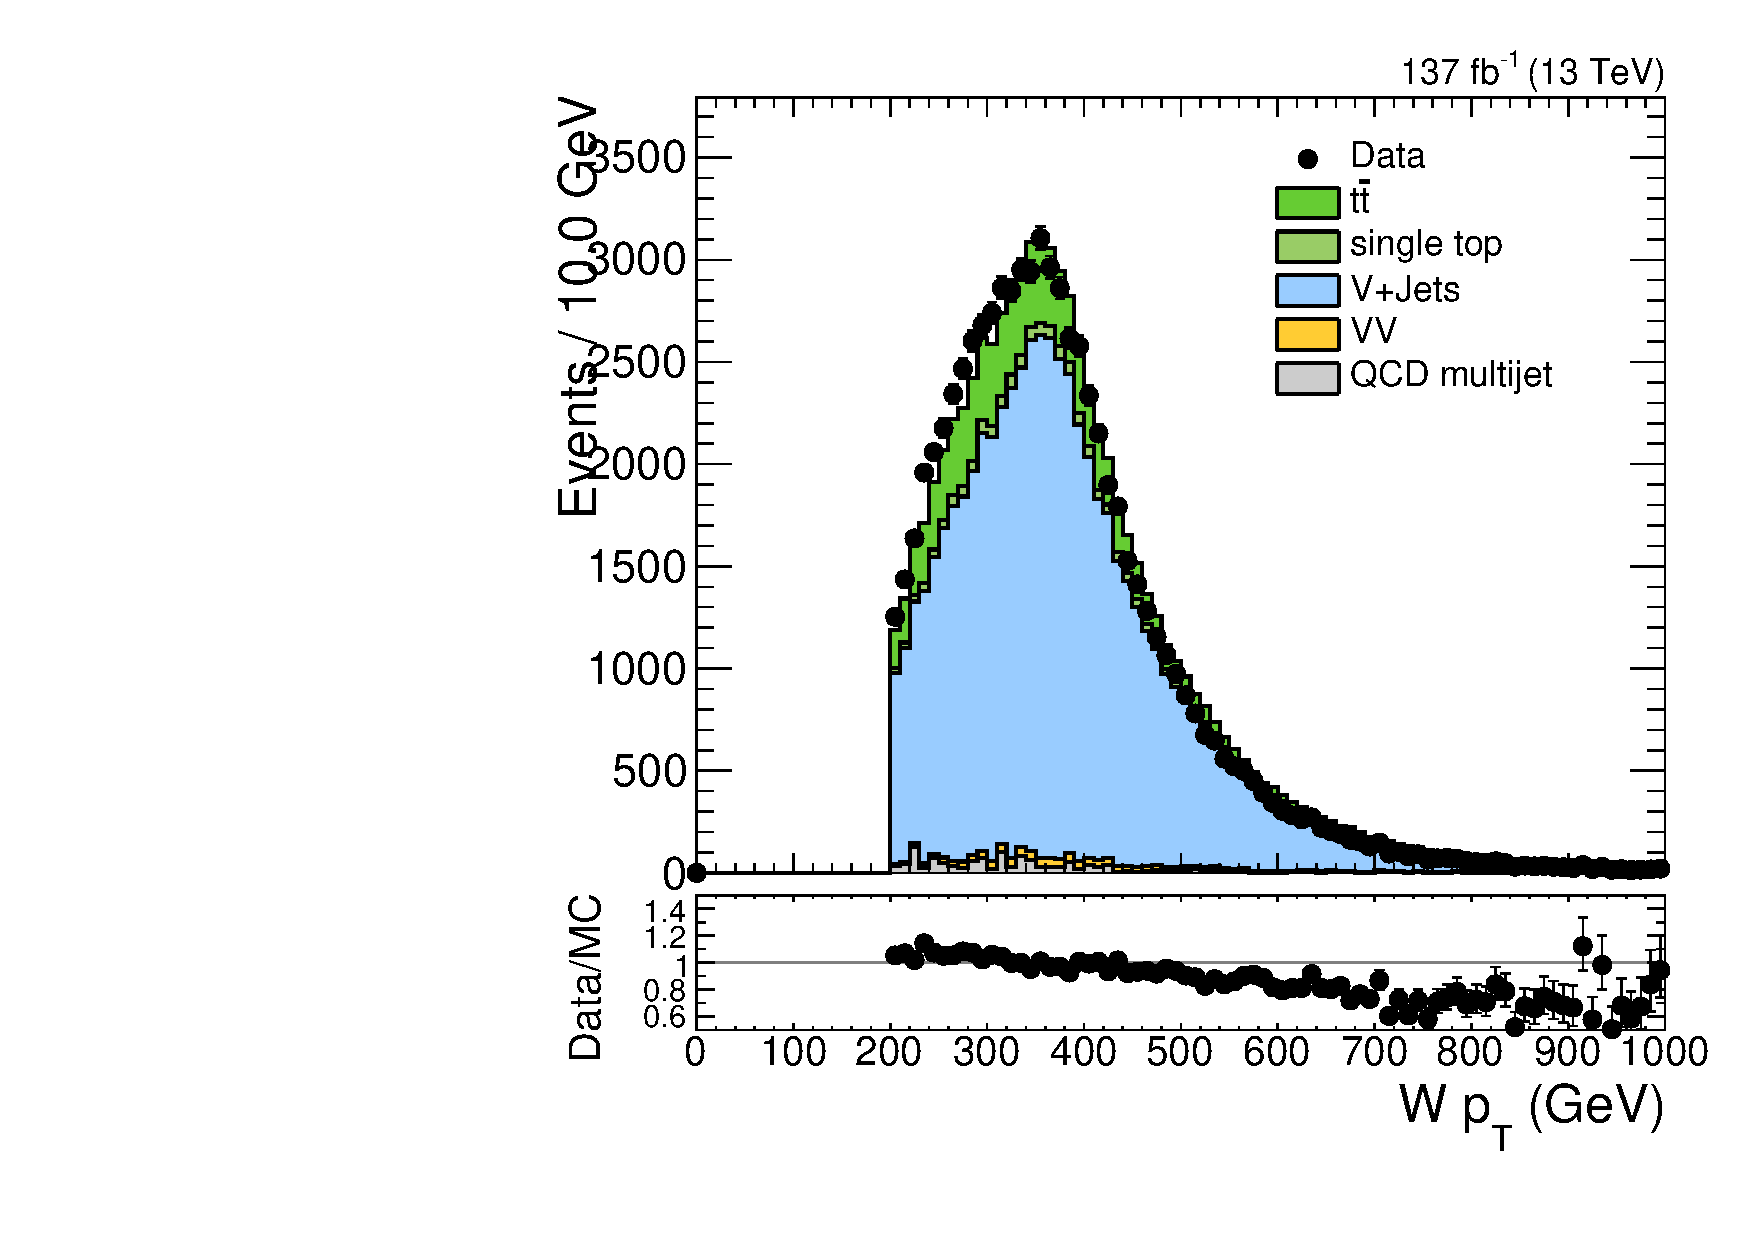
\includegraphics[width=0.3825\textwidth]{fig/analysisAppendix/SB_b1_e_allP_allC_allD_Run2_lnujj_l1_pt.pdf}\\
  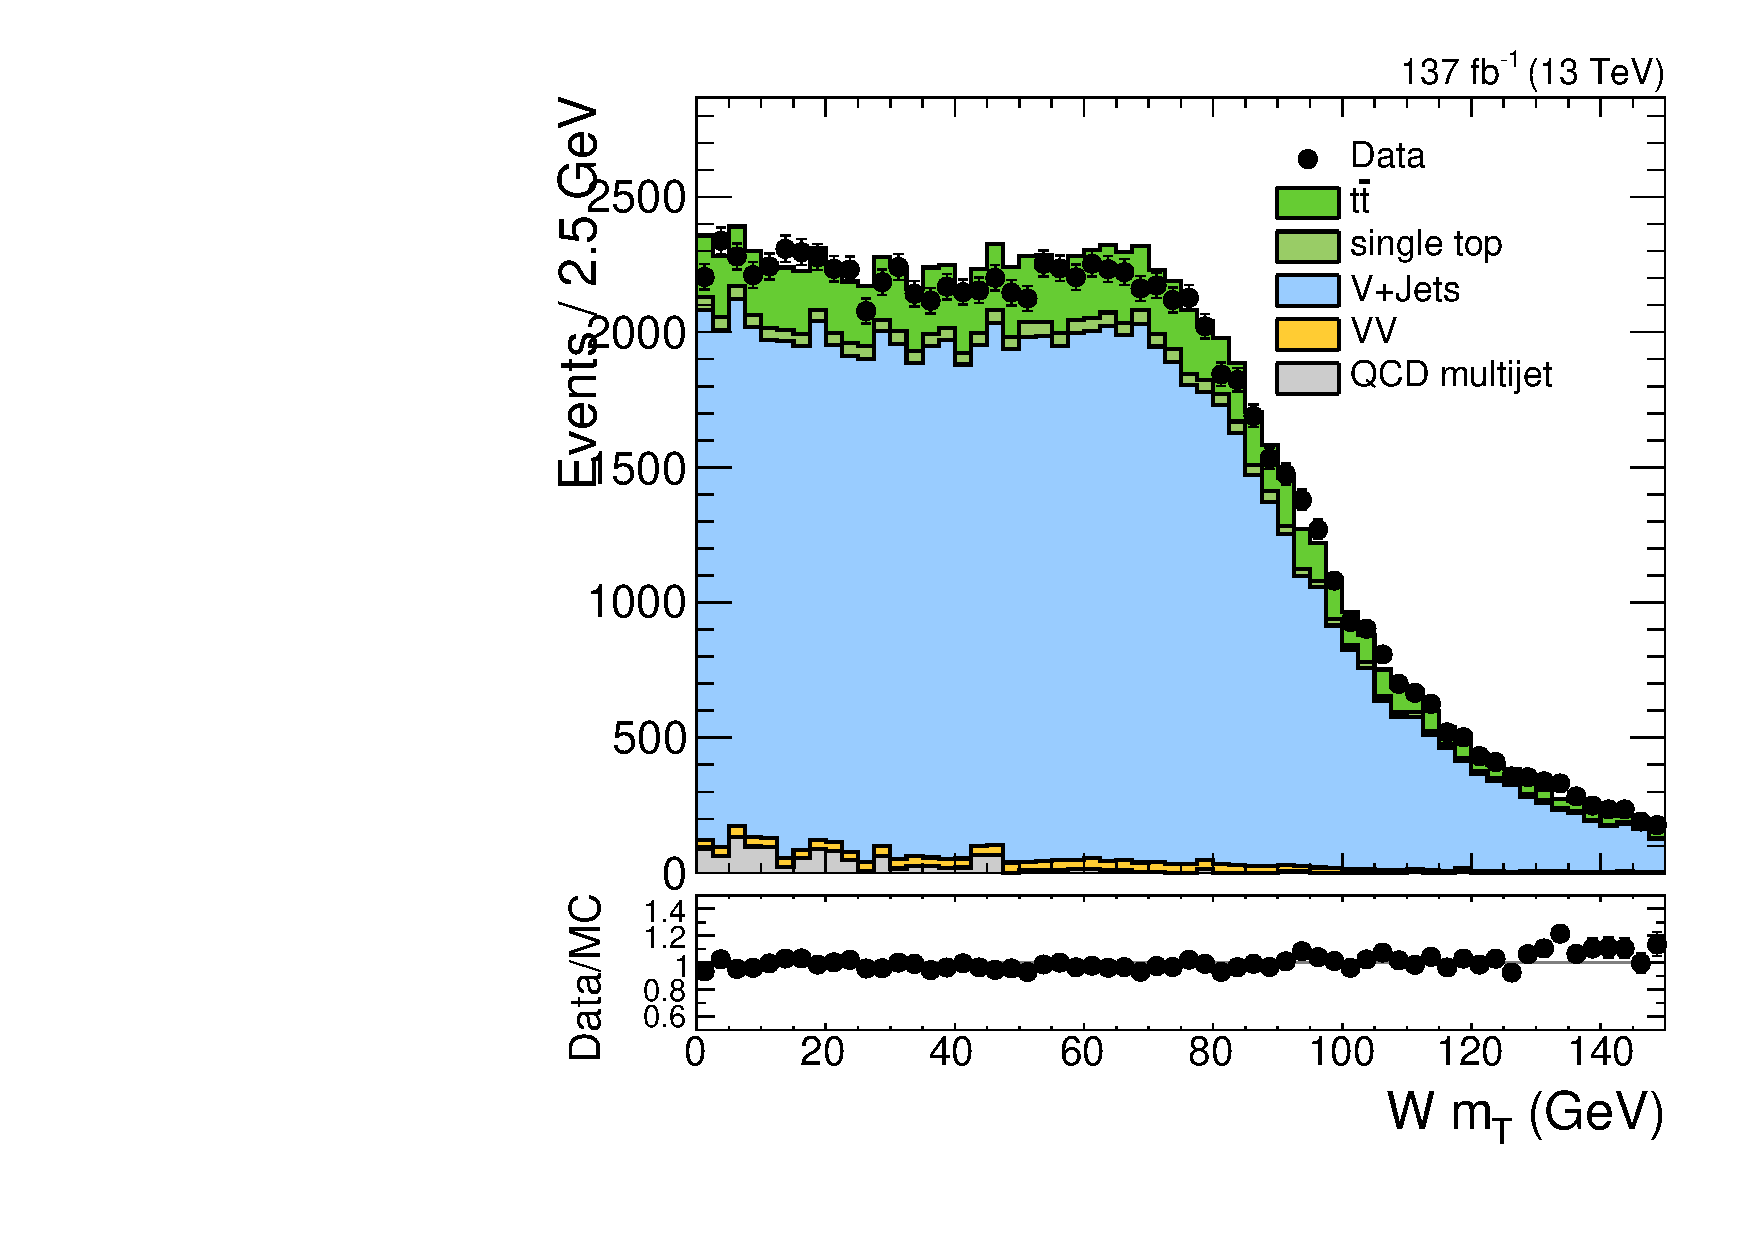
\includegraphics[width=0.3825\textwidth]{fig/analysisAppendix/SB_b1_mu_allP_allC_allD_Run2_lnujj_l1_mt.pdf}
  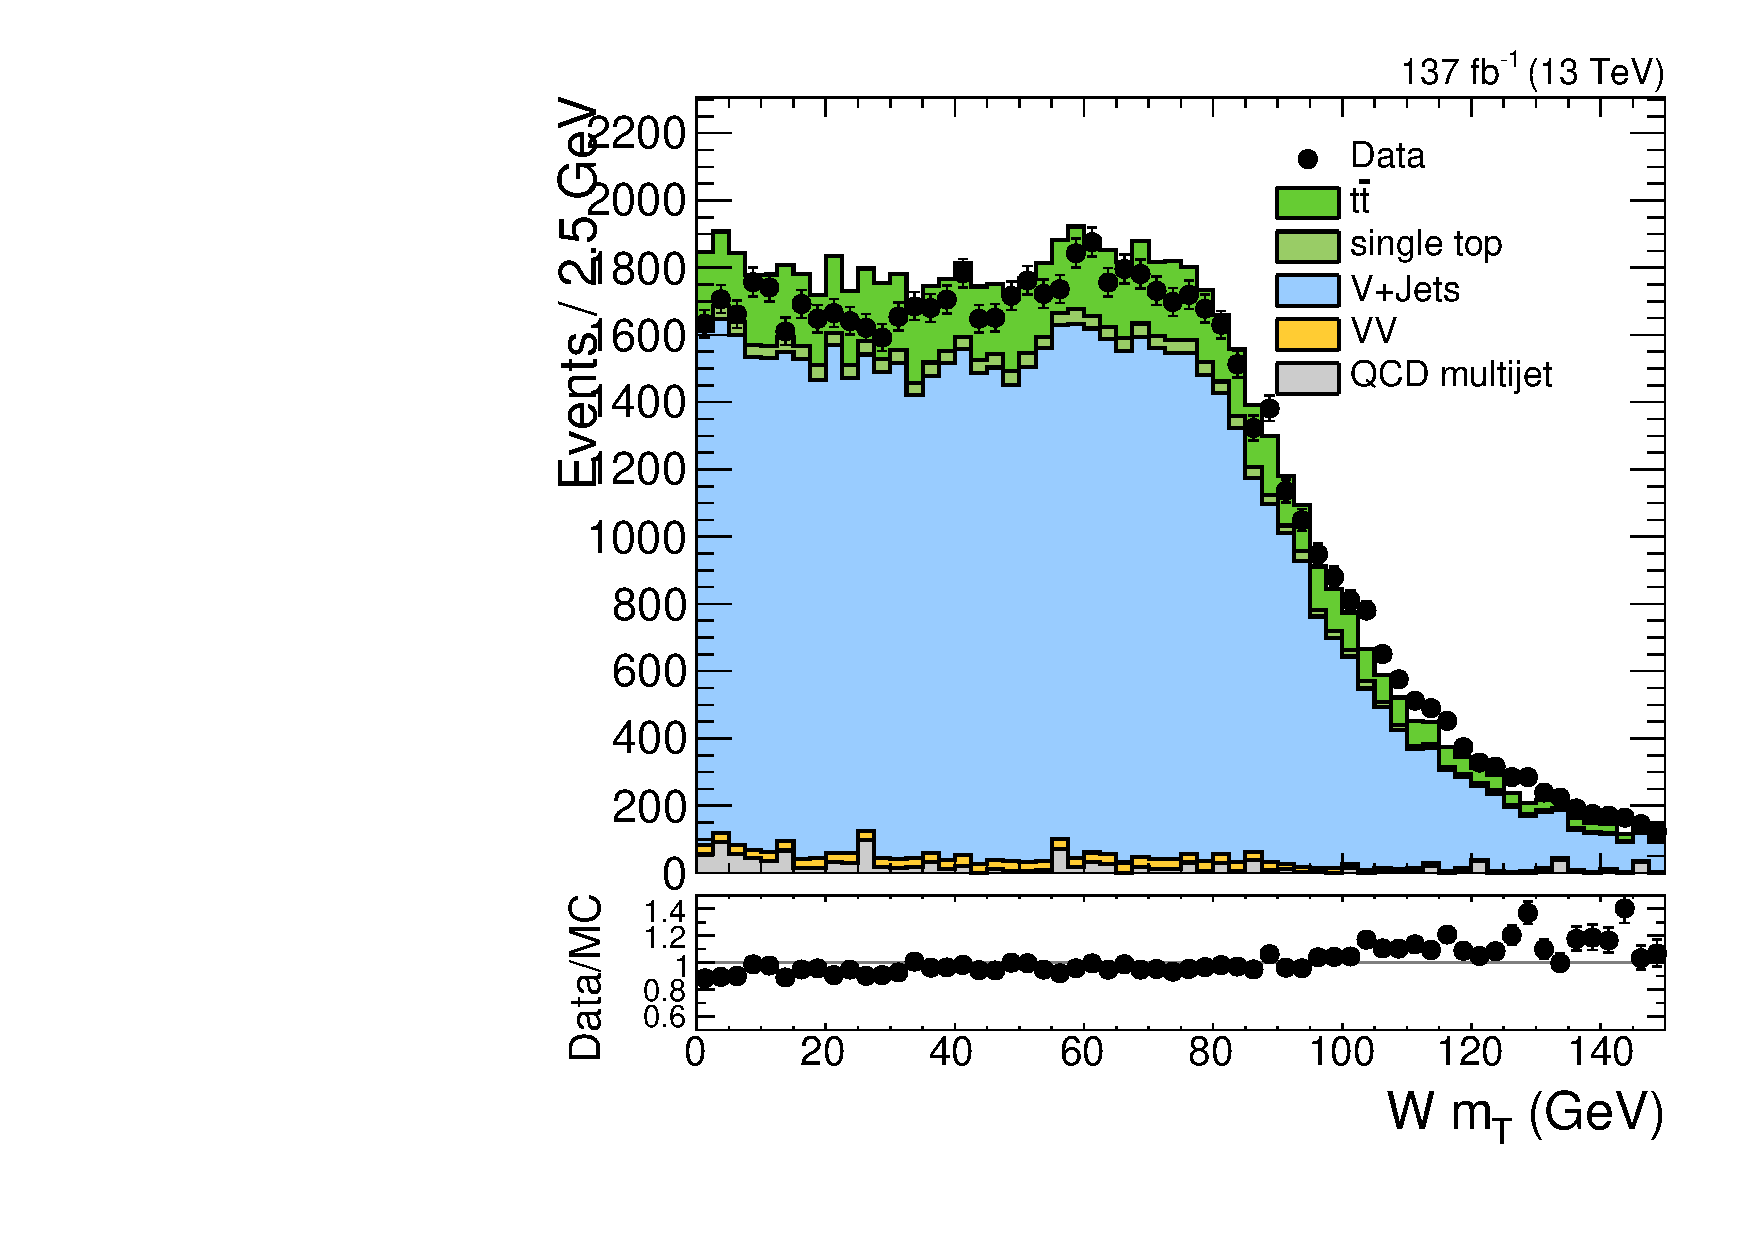
\includegraphics[width=0.3825\textwidth]{fig/analysisAppendix/SB_b1_e_allP_allC_allD_Run2_lnujj_l1_mt.pdf}\\
  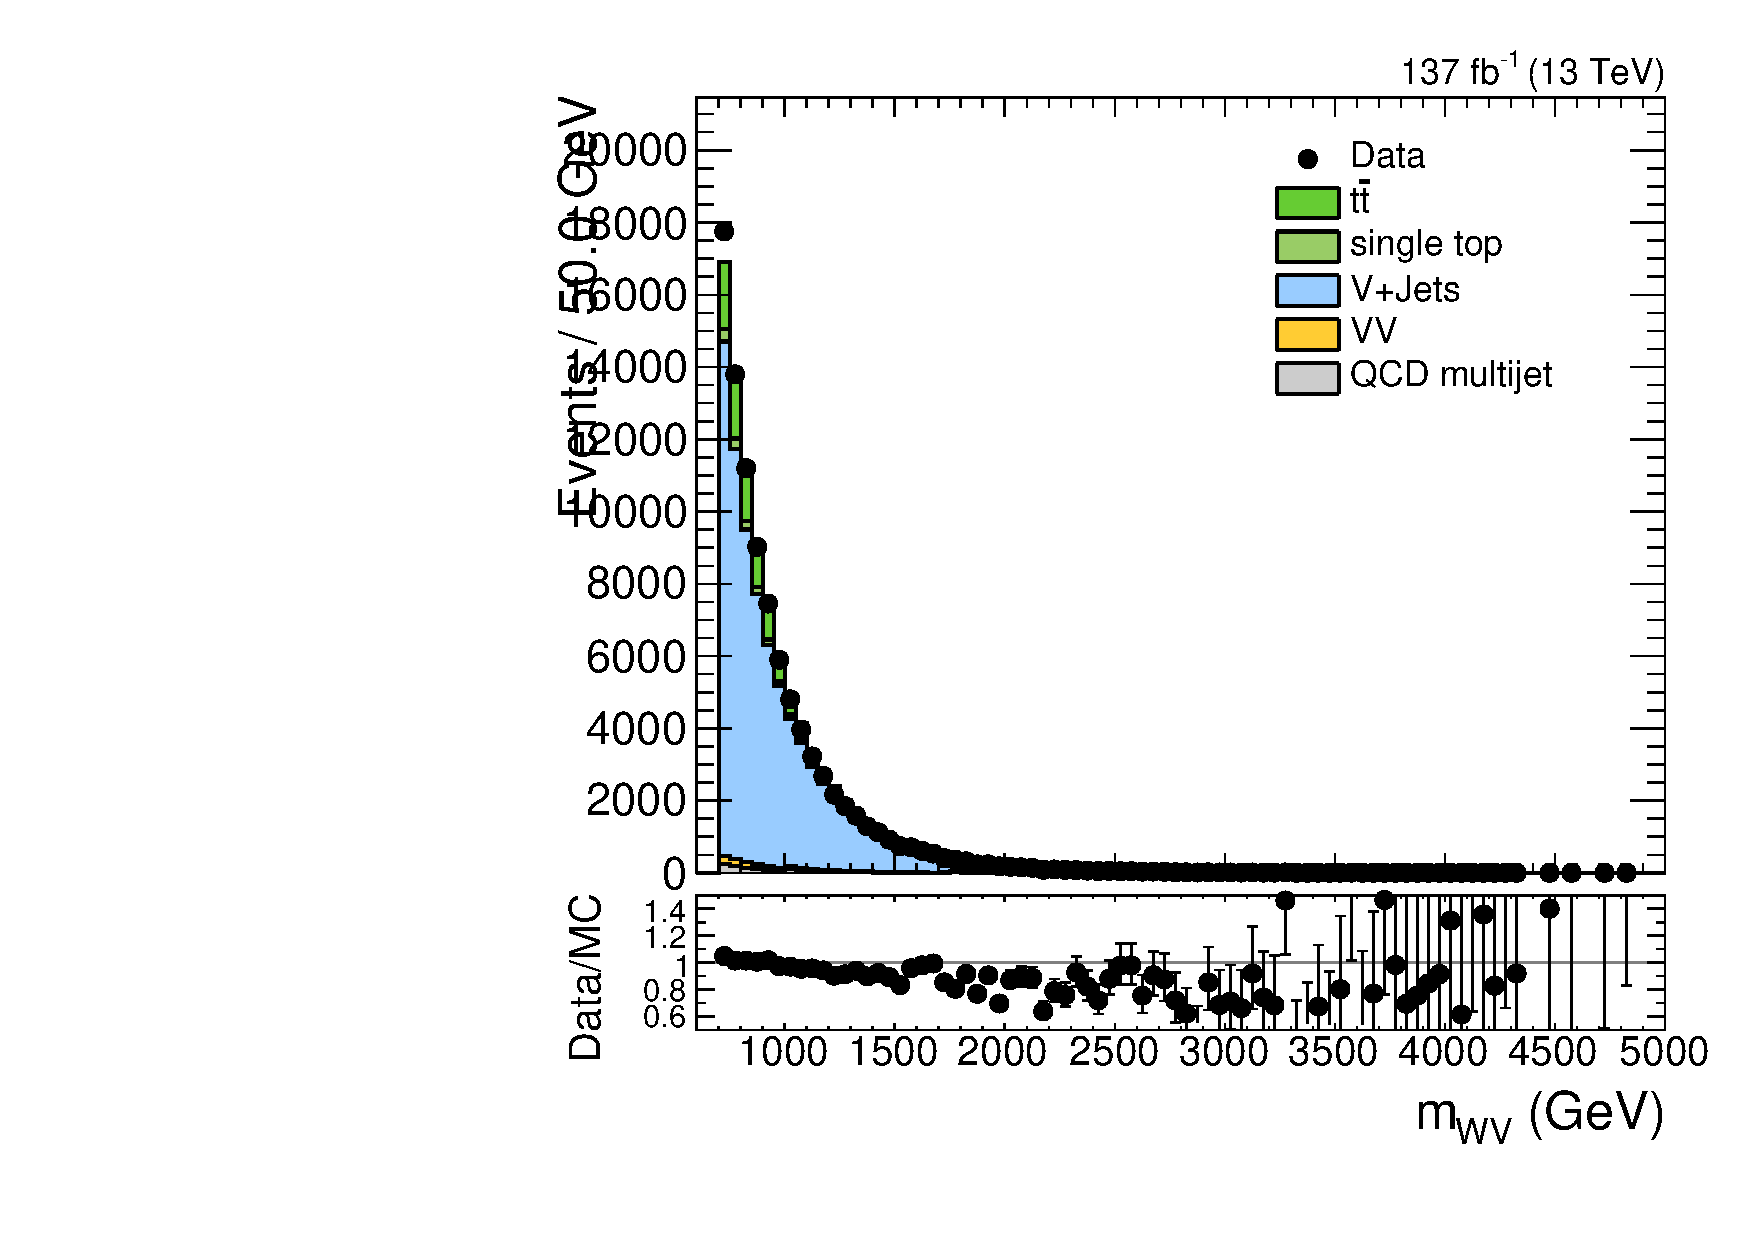
\includegraphics[width=0.3825\textwidth]{fig/analysisAppendix/SB_b1_mu_allP_allC_allD_Run2_mWV.pdf}
  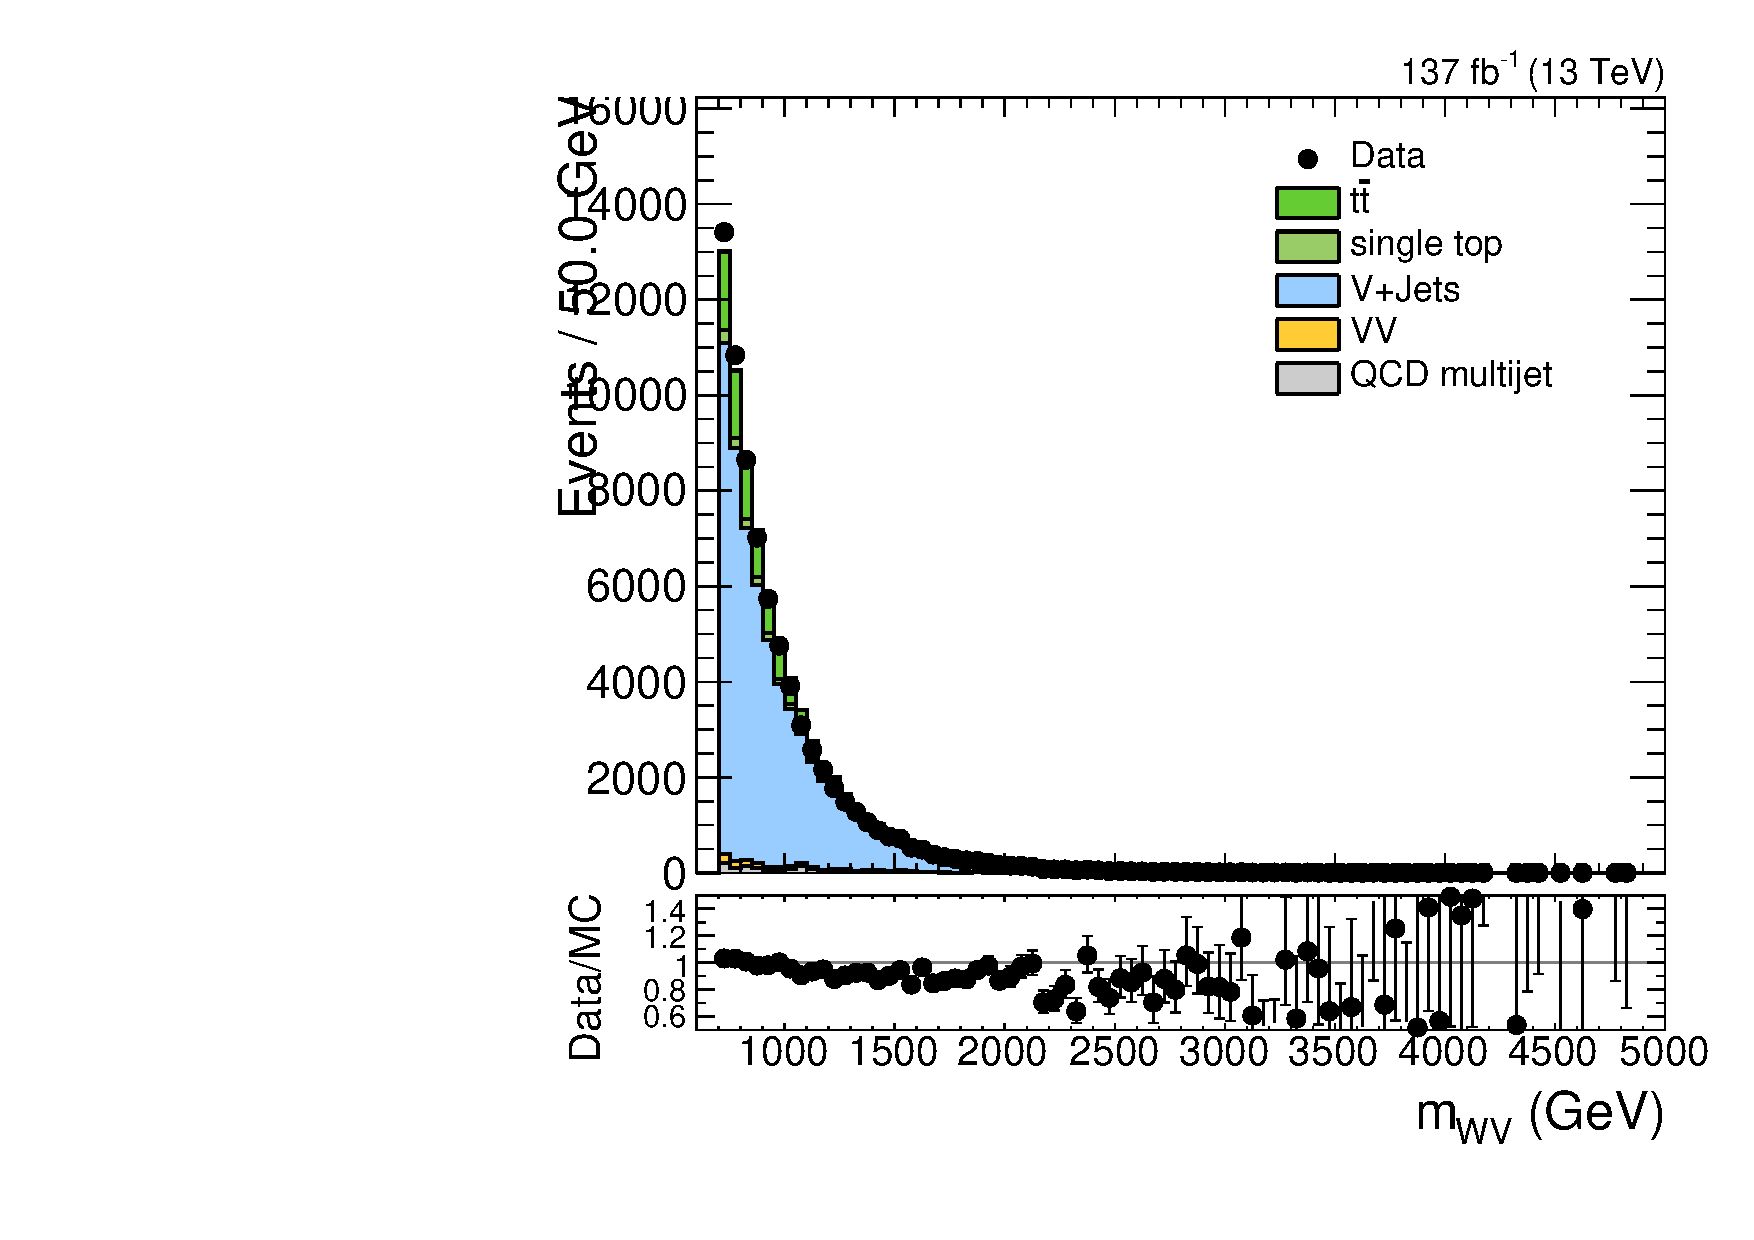
\includegraphics[width=0.3825\textwidth]{fig/analysisAppendix/SB_b1_e_allP_allC_allD_Run2_mWV.pdf}\\
  \caption{
    Comparison plots between data and MC from Run 2 for different \Wlep-related observables, in the jet mass sideband.
    From top to bottom: \pt of the leptonic $W$, transverse mass of the leptonic $W$, diboson invariant mass.
    Left: muon channel, right: electron channel.
  }
  \label{fig:SB_controlPlotsRun2_2}
\end{figure}

\begin{figure}[htbp]
  \centering
  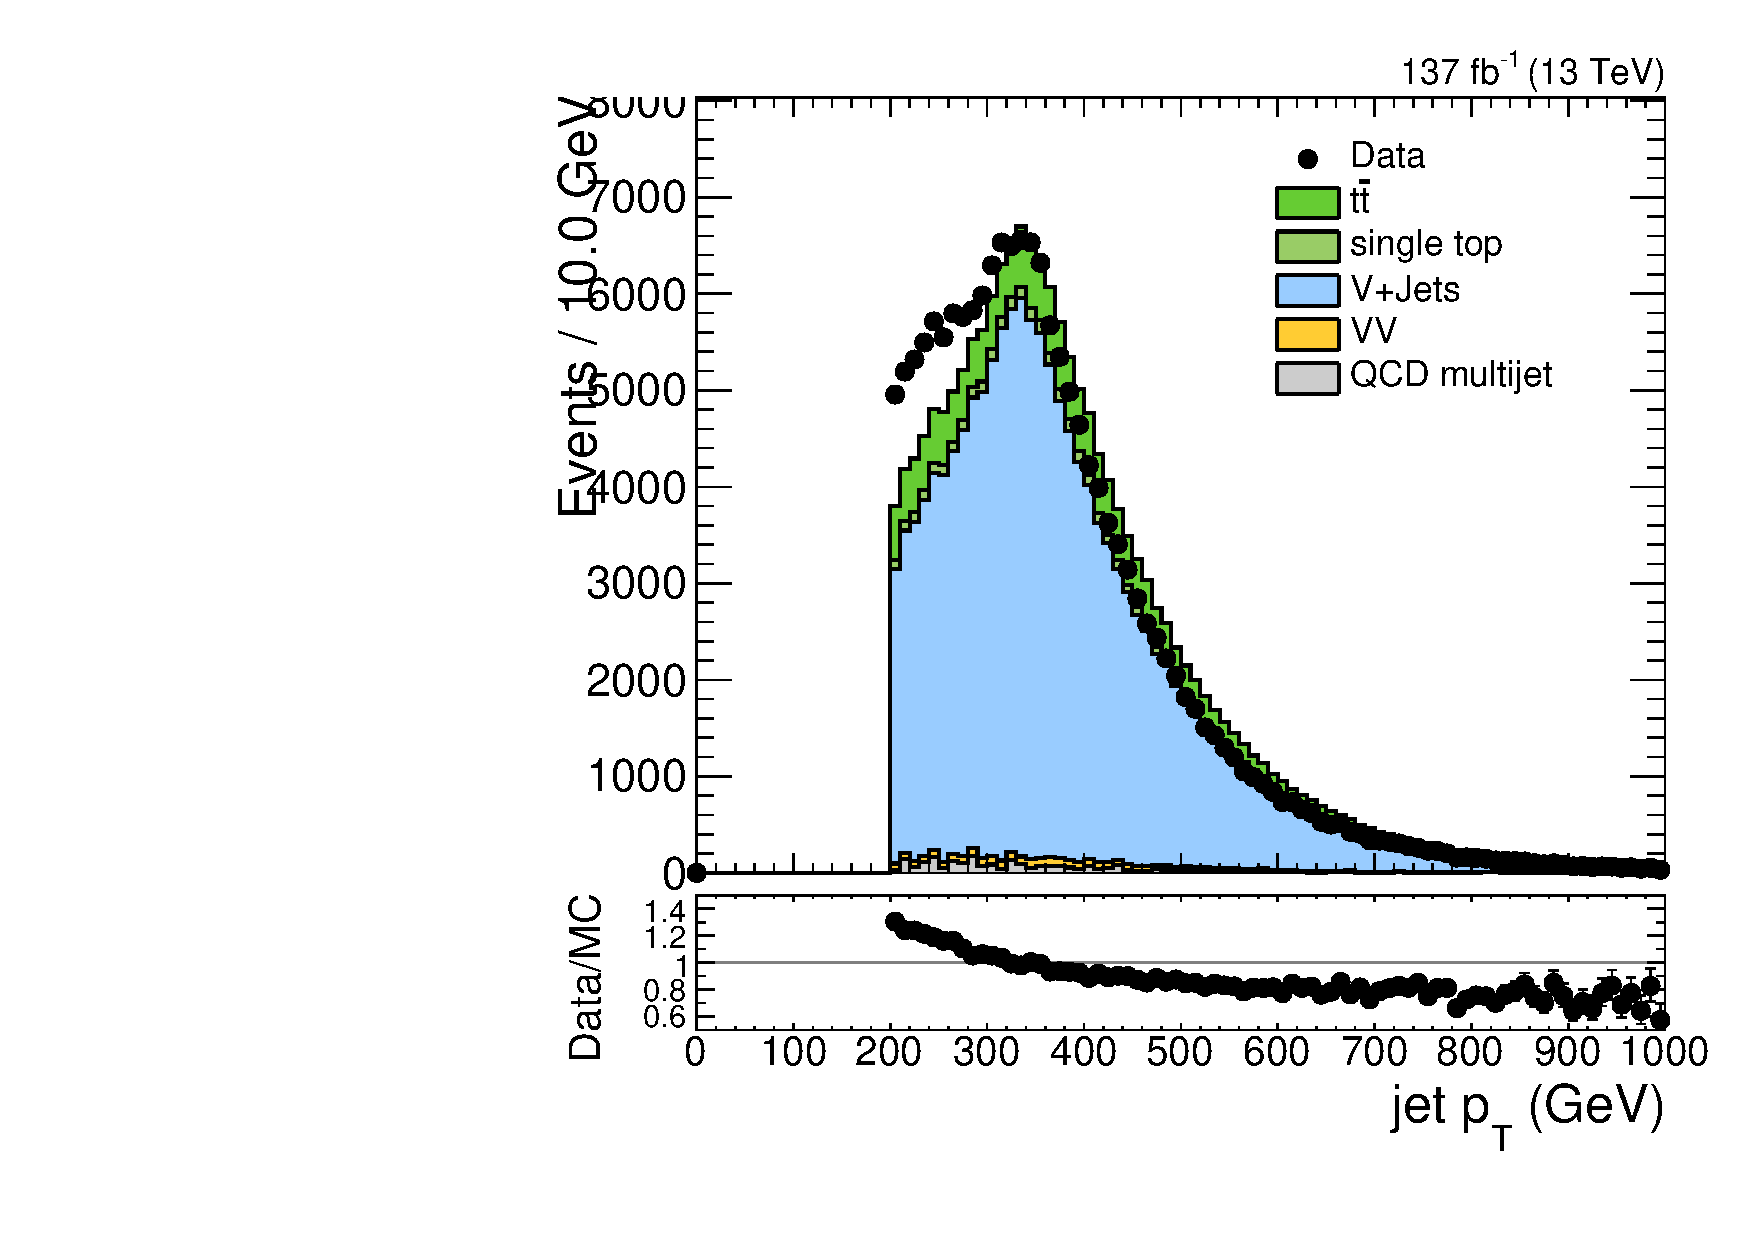
\includegraphics[width=0.3825\textwidth]{fig/analysisAppendix/SB_b1_allL_allP_allC_allD_Run2_lnujj_l2_pt.pdf}
  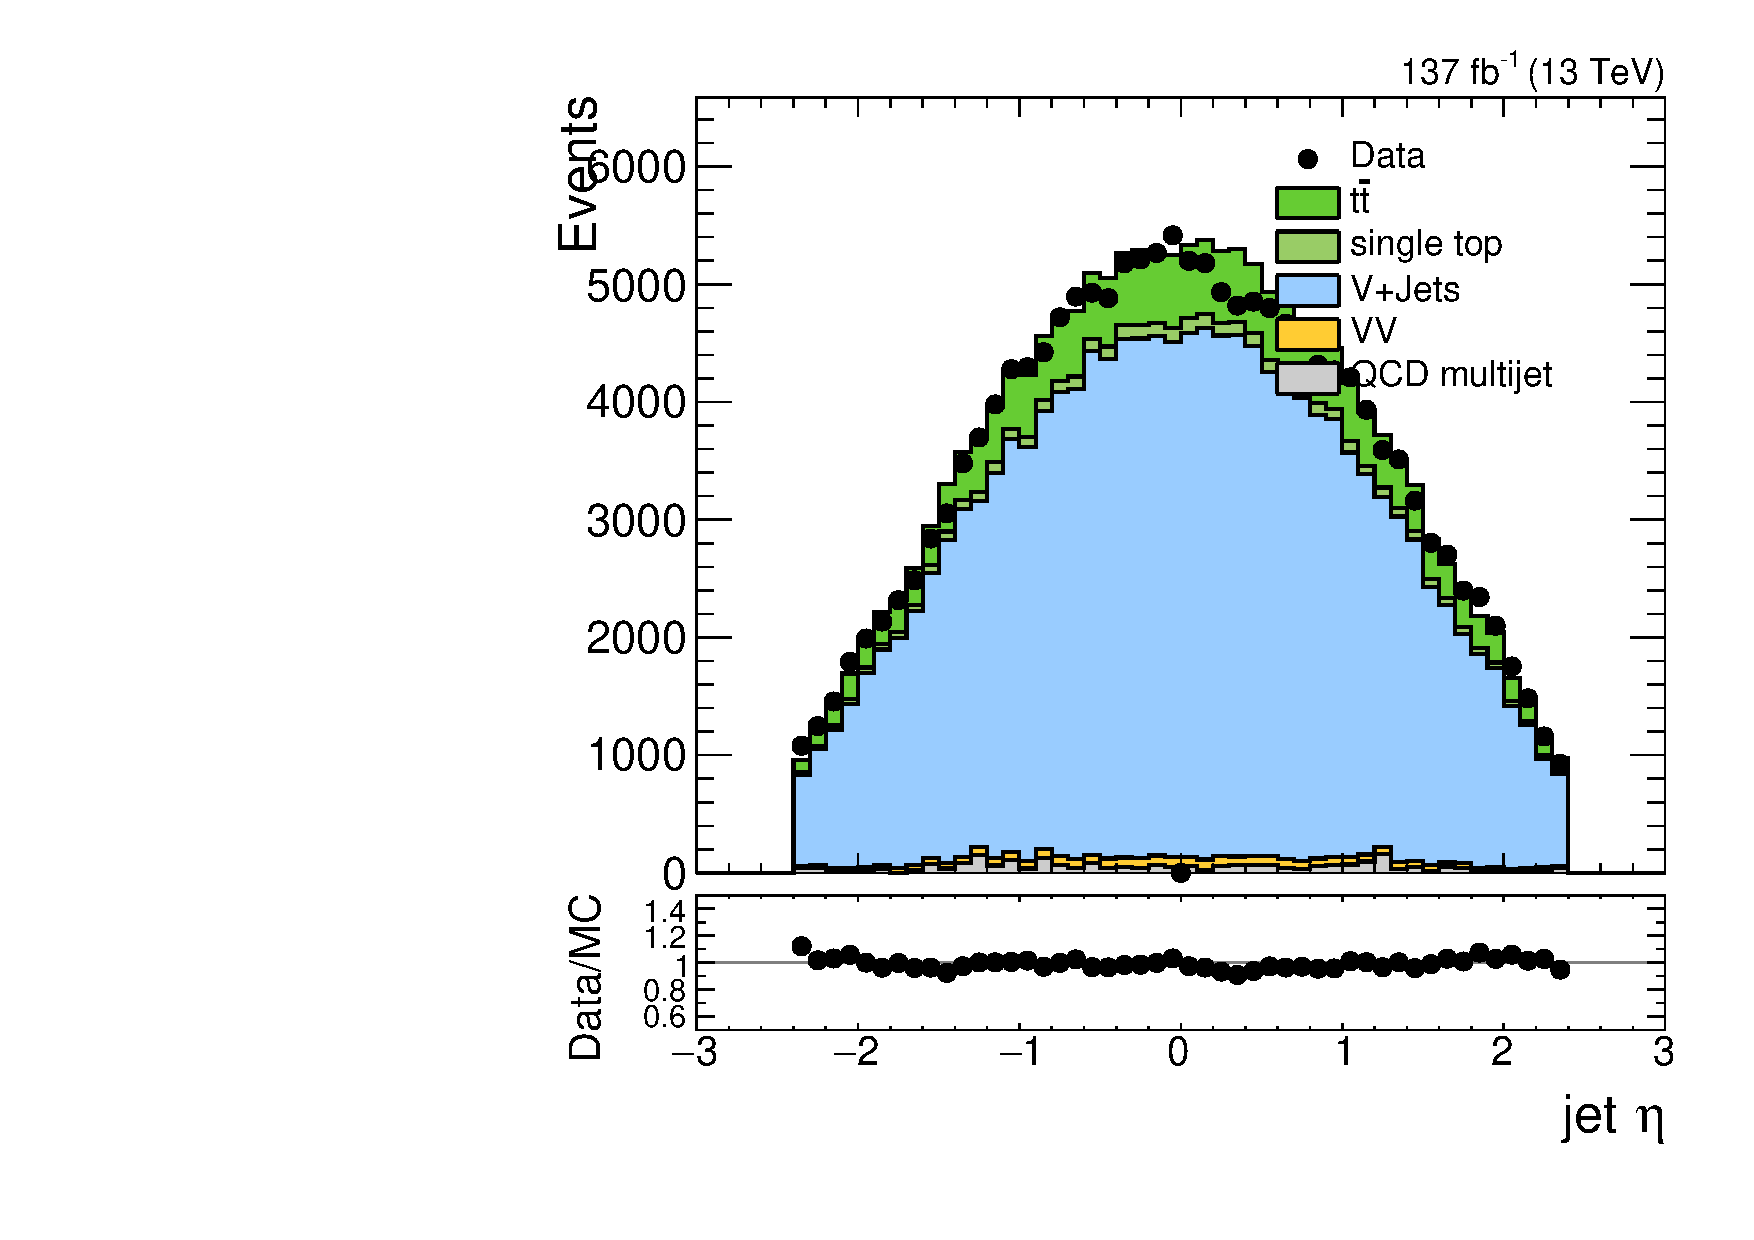
\includegraphics[width=0.3825\textwidth]{fig/analysisAppendix/SB_b1_allL_allP_allC_allD_Run2_lnujj_l2_eta.pdf}\\
  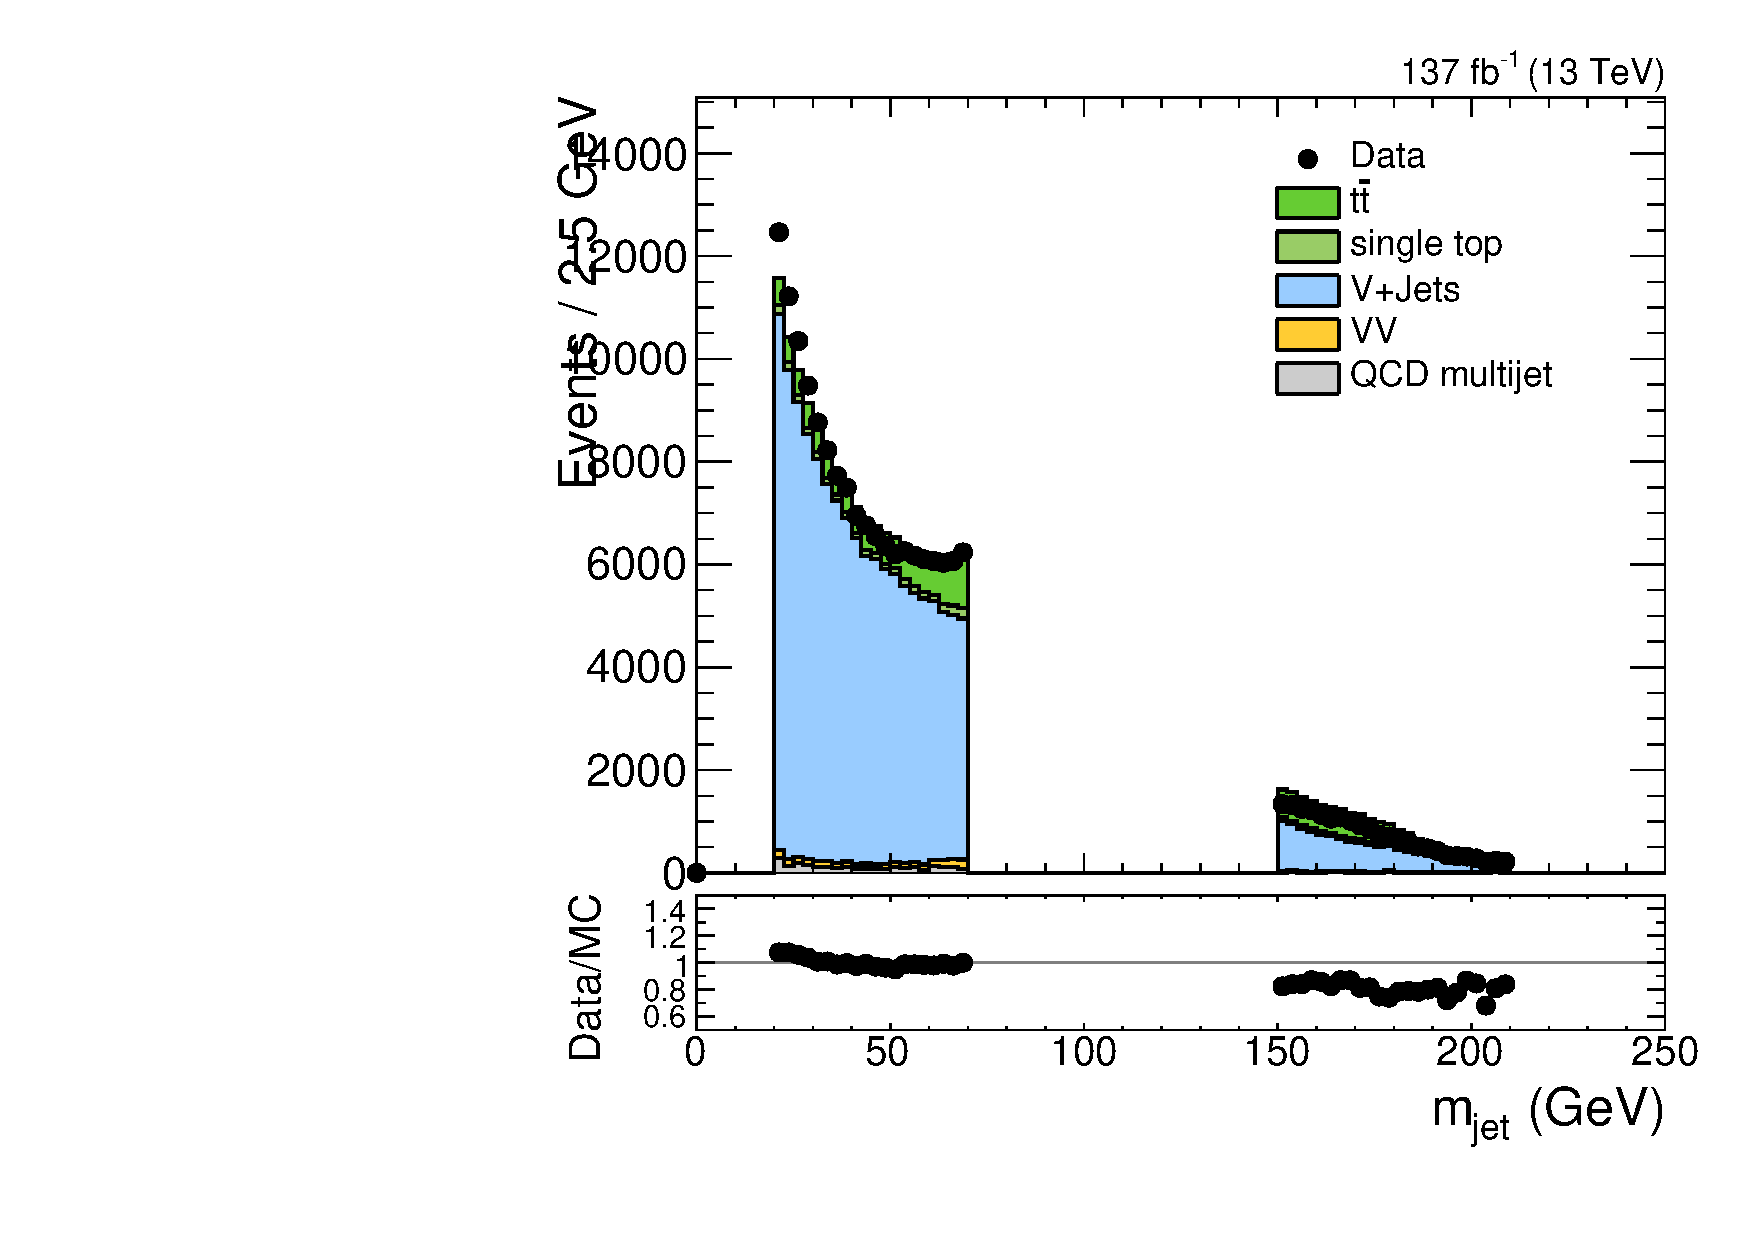
\includegraphics[width=0.3825\textwidth]{fig/analysisAppendix/SB_b1_allL_allP_allC_allD_Run2_mjet.pdf}\\
  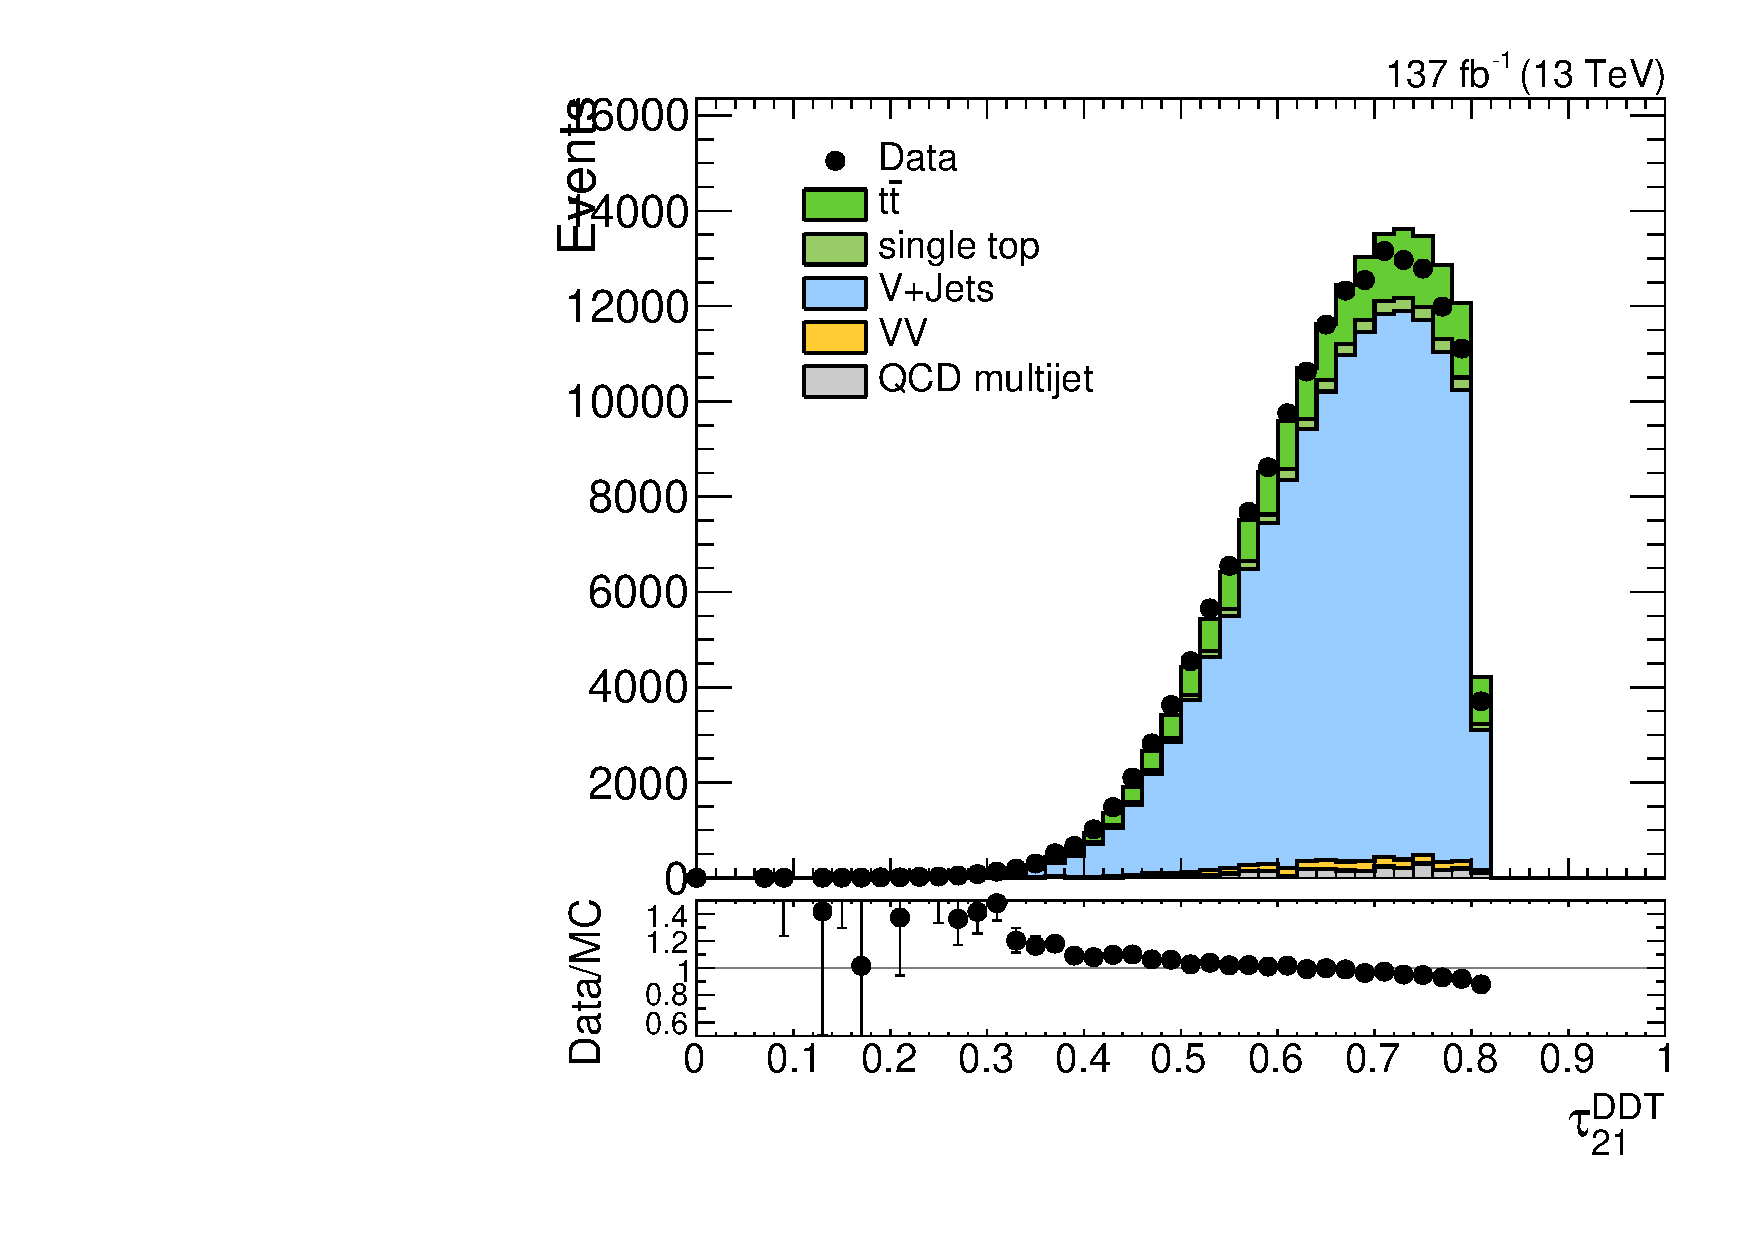
\includegraphics[width=0.3825\textwidth]{fig/analysisAppendix/SB_b1_allL_allP_allC_allD_Run2_tau21DDT.pdf}
  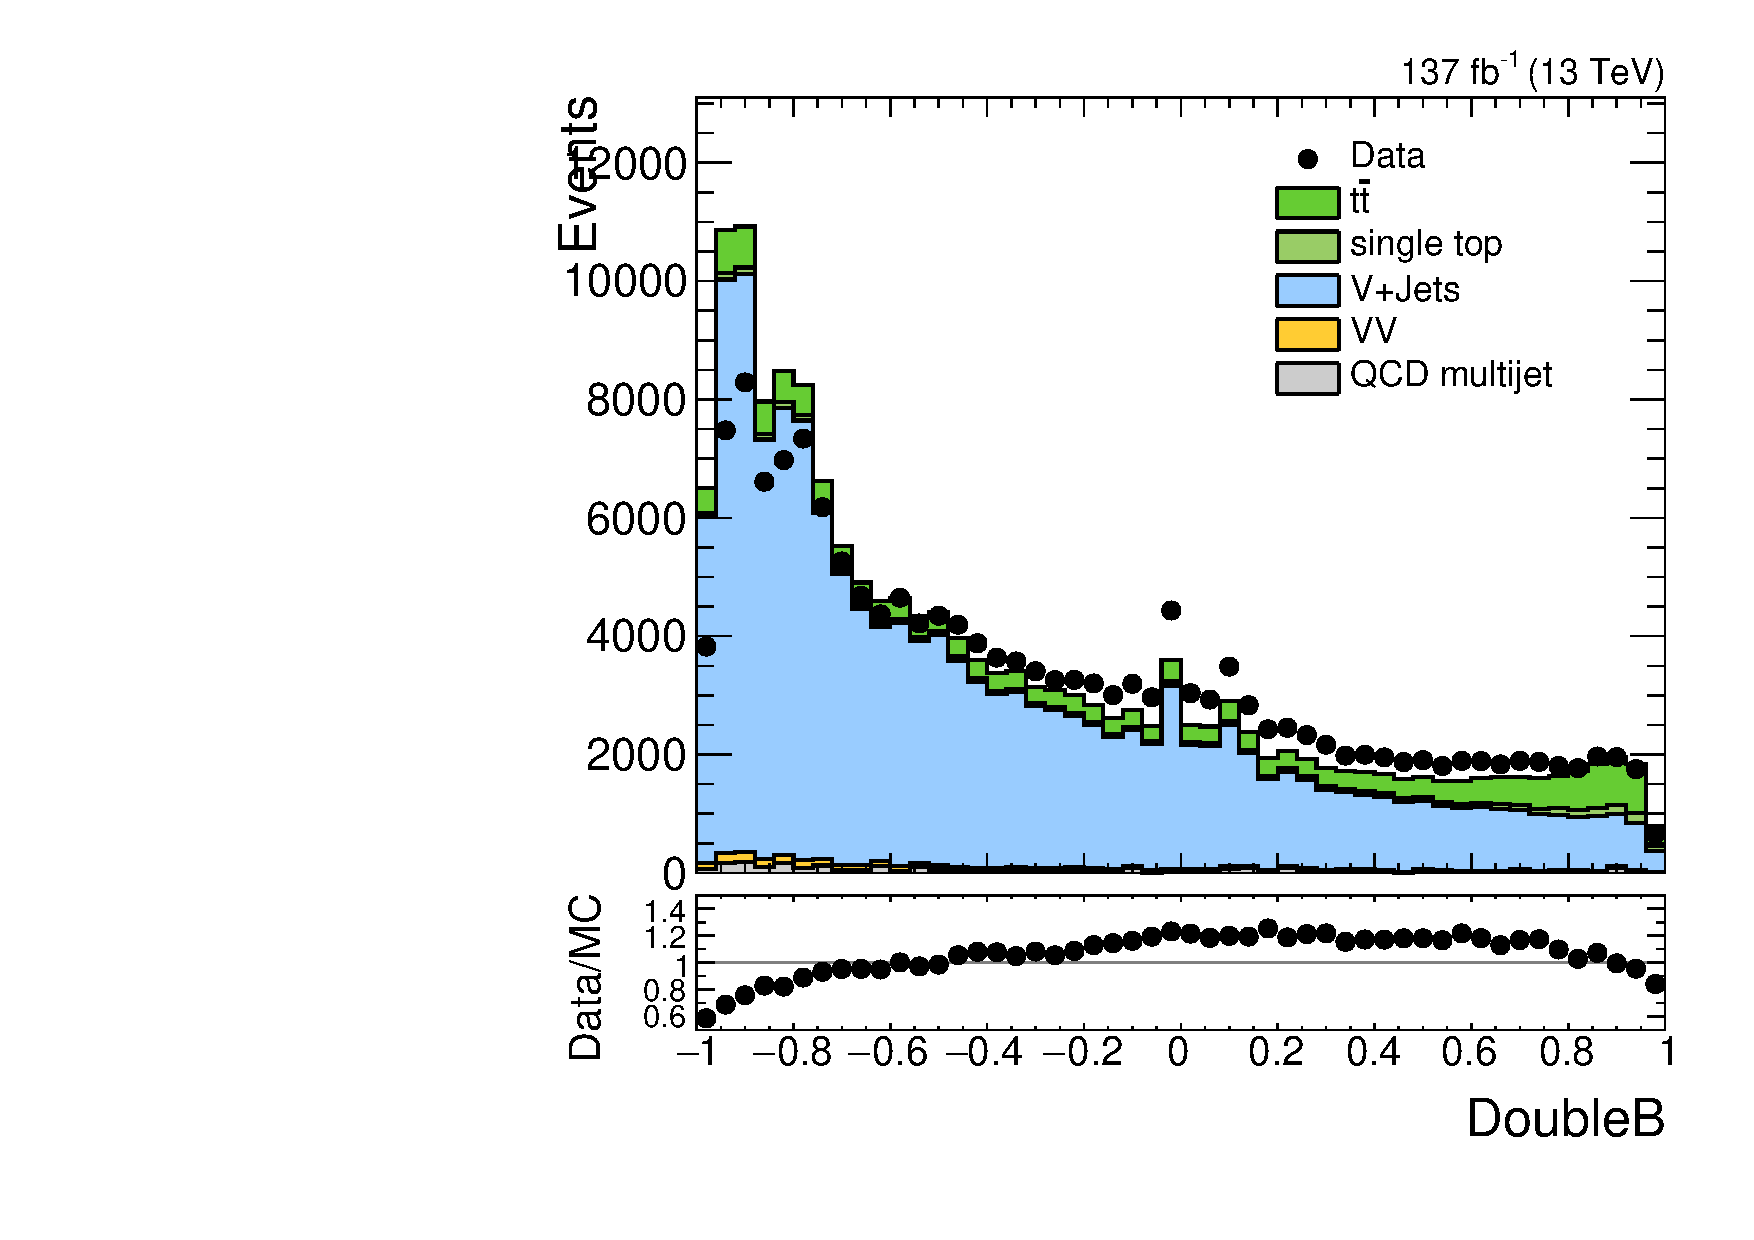
\includegraphics[width=0.3825\textwidth]{fig/analysisAppendix/SB_b1_allL_allP_allC_allD_Run2_DoubleB.pdf}\\
  \caption{
    Comparison plots between data and MC from Run 2 for the \pt, $\eta$, \MJ (soft drop mass), \nsubjDDT, and \DoubleB tagger of the selected \Vhad candidate (leading AK8 jet), in the jet mass sideband.
  }
  \label{fig:SB_controlPlotsRun2_3}
\end{figure}

\begin{figure}[htbp]
  \centering
  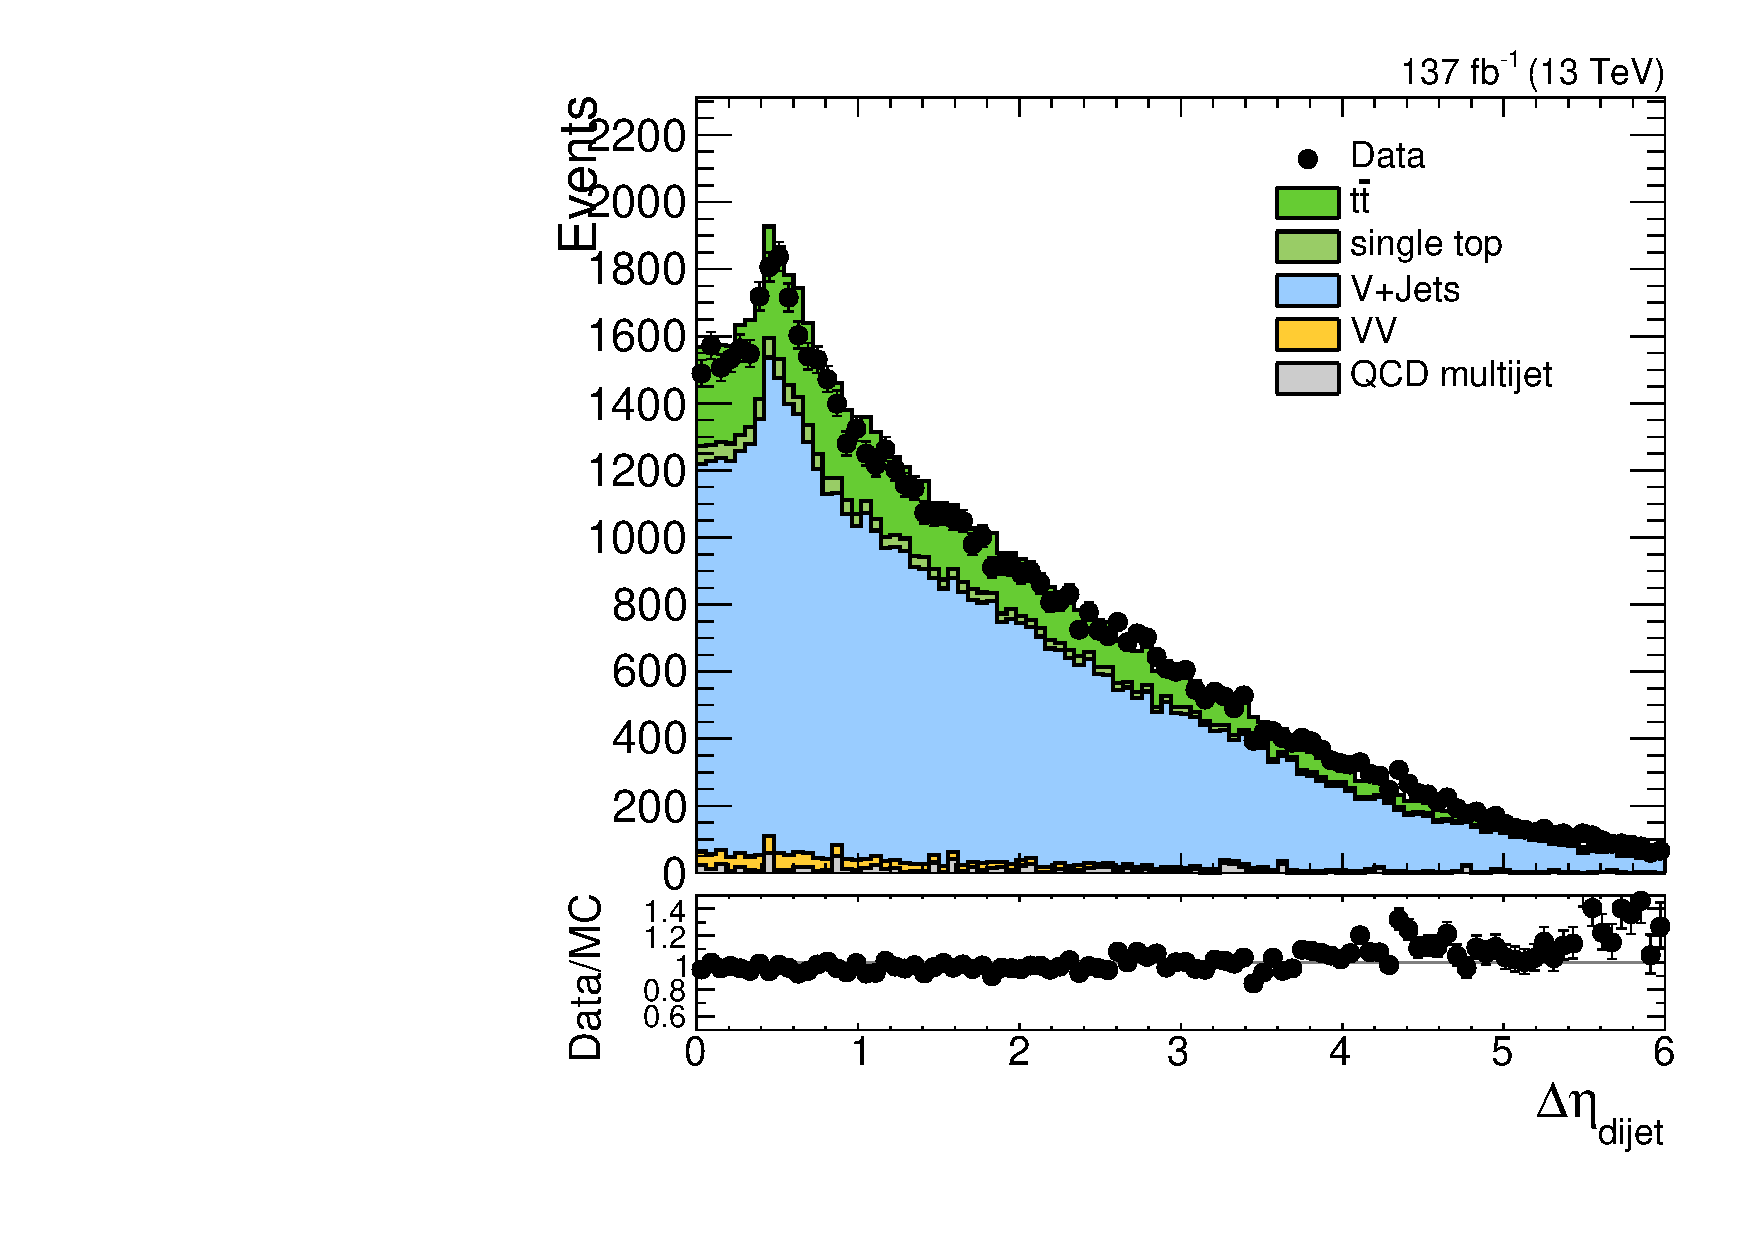
\includegraphics[width=0.3825\textwidth]{fig/analysisAppendix/SB_b1_allL_allP_allC_allD_Run2_lnujj_vbfDEta.pdf}
  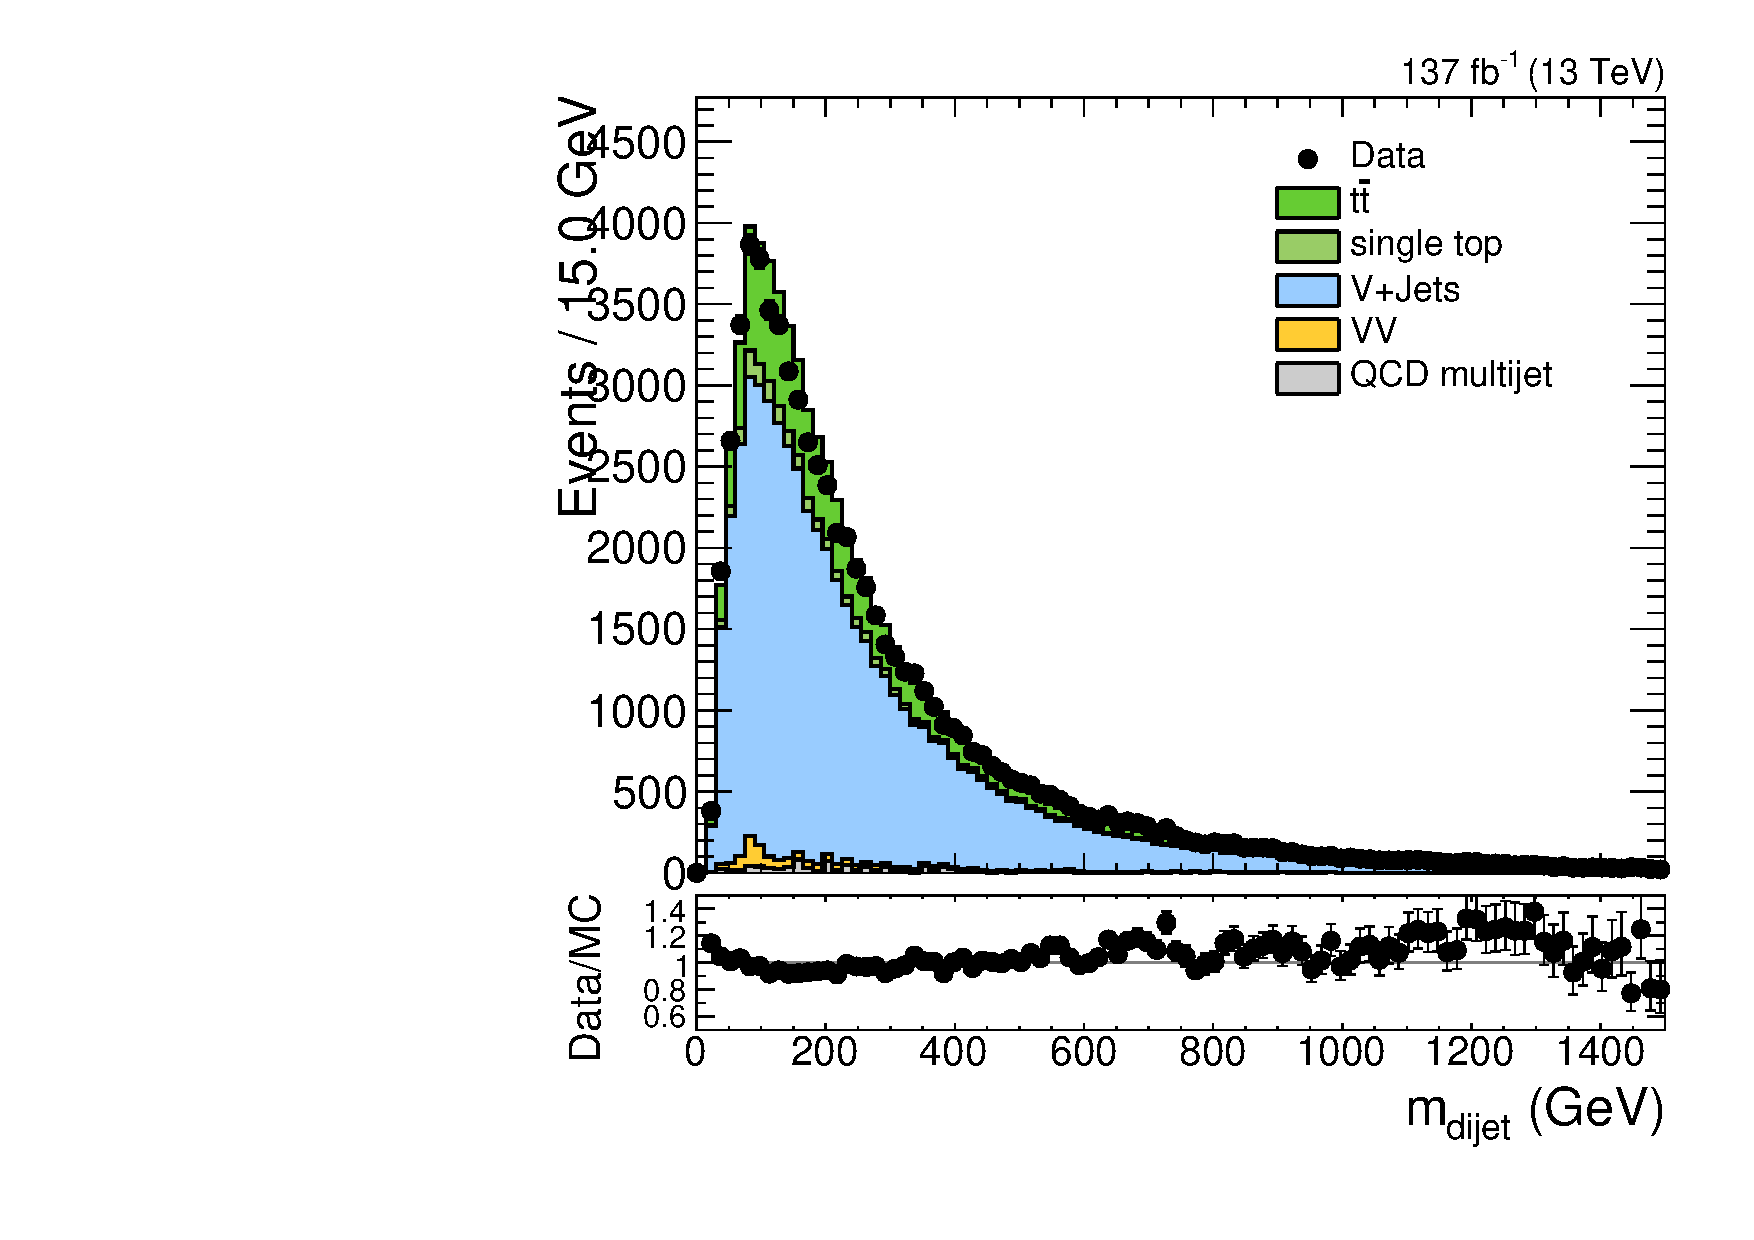
\includegraphics[width=0.3825\textwidth]{fig/analysisAppendix/SB_b1_allL_allP_allC_allD_Run2_lnujj_vbfMass.pdf}\\
  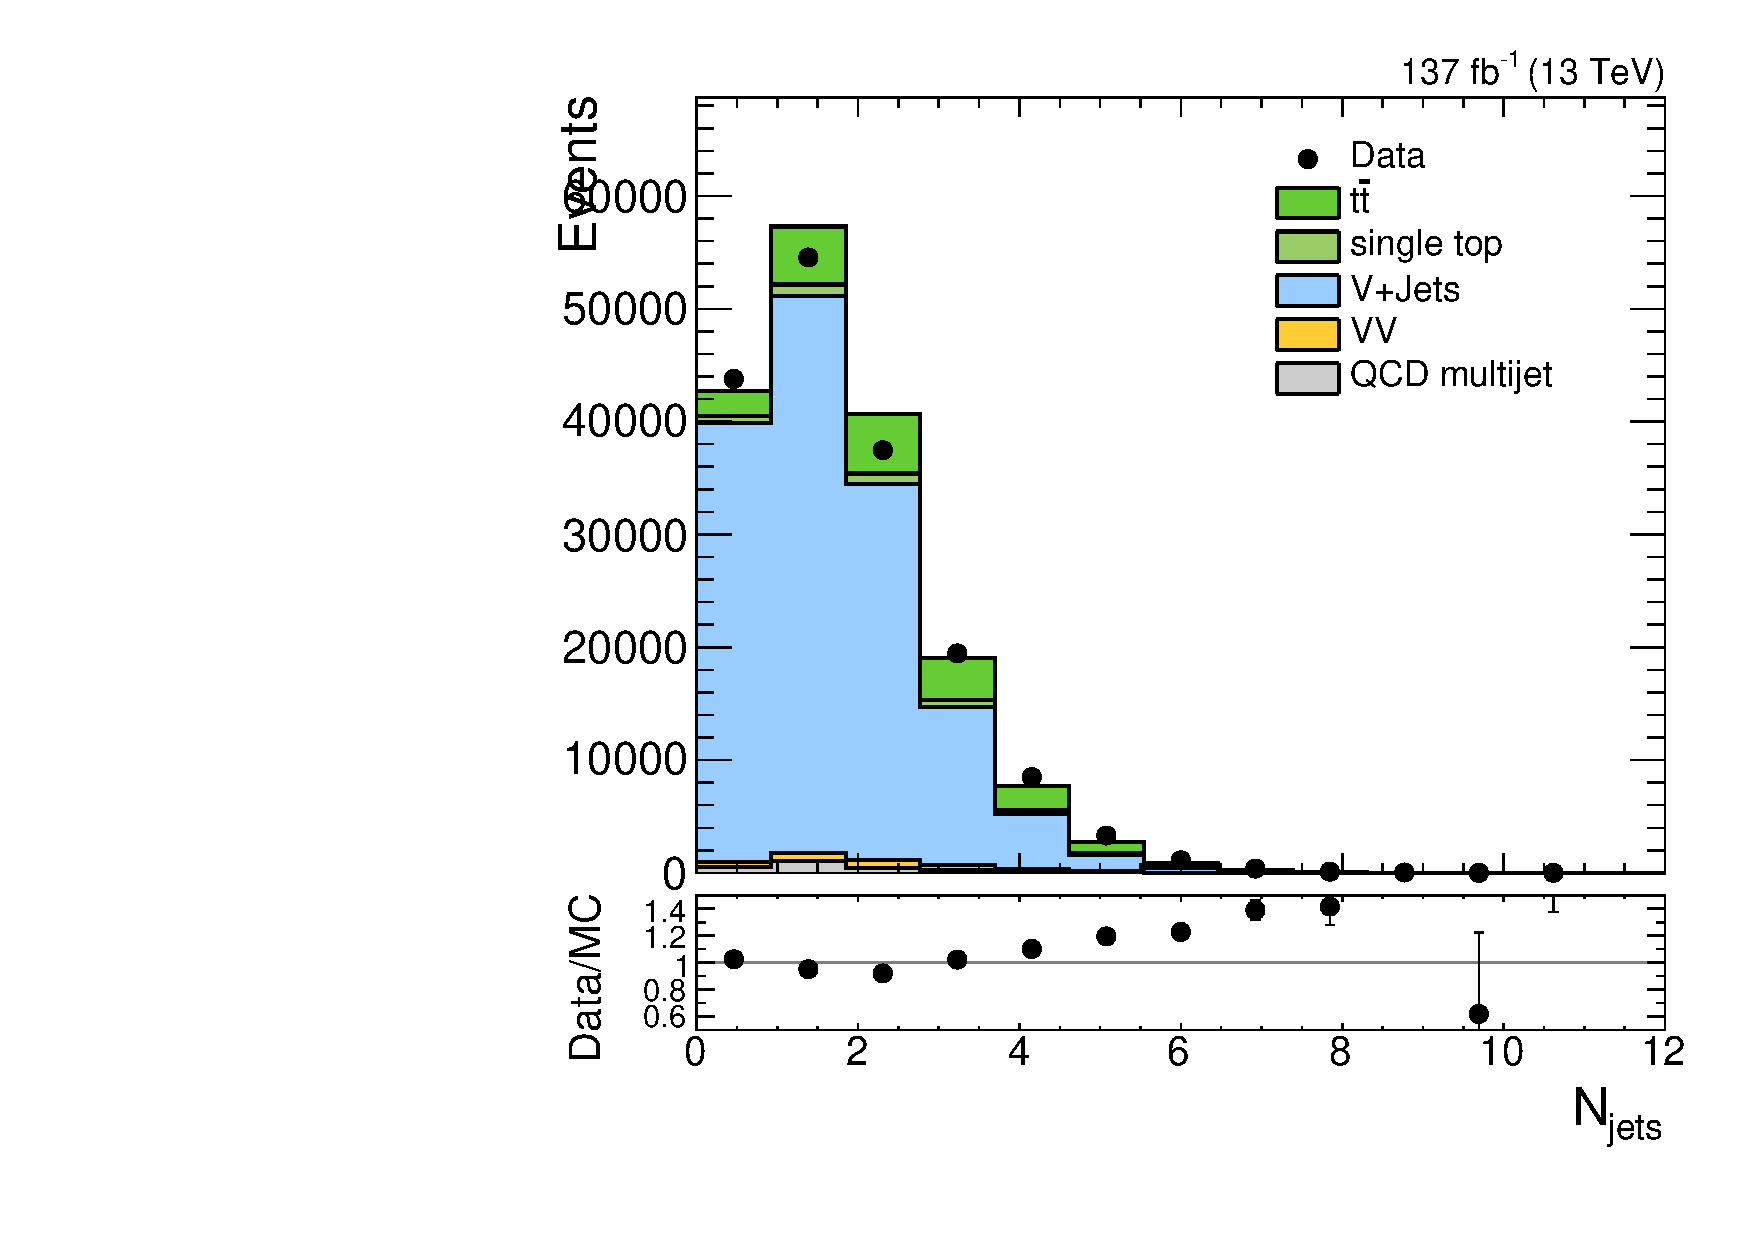
\includegraphics[width=0.3825\textwidth]{fig/analysisAppendix/SB_b1_allL_allP_allC_allD_Run2_lnujj_nJets.pdf}
  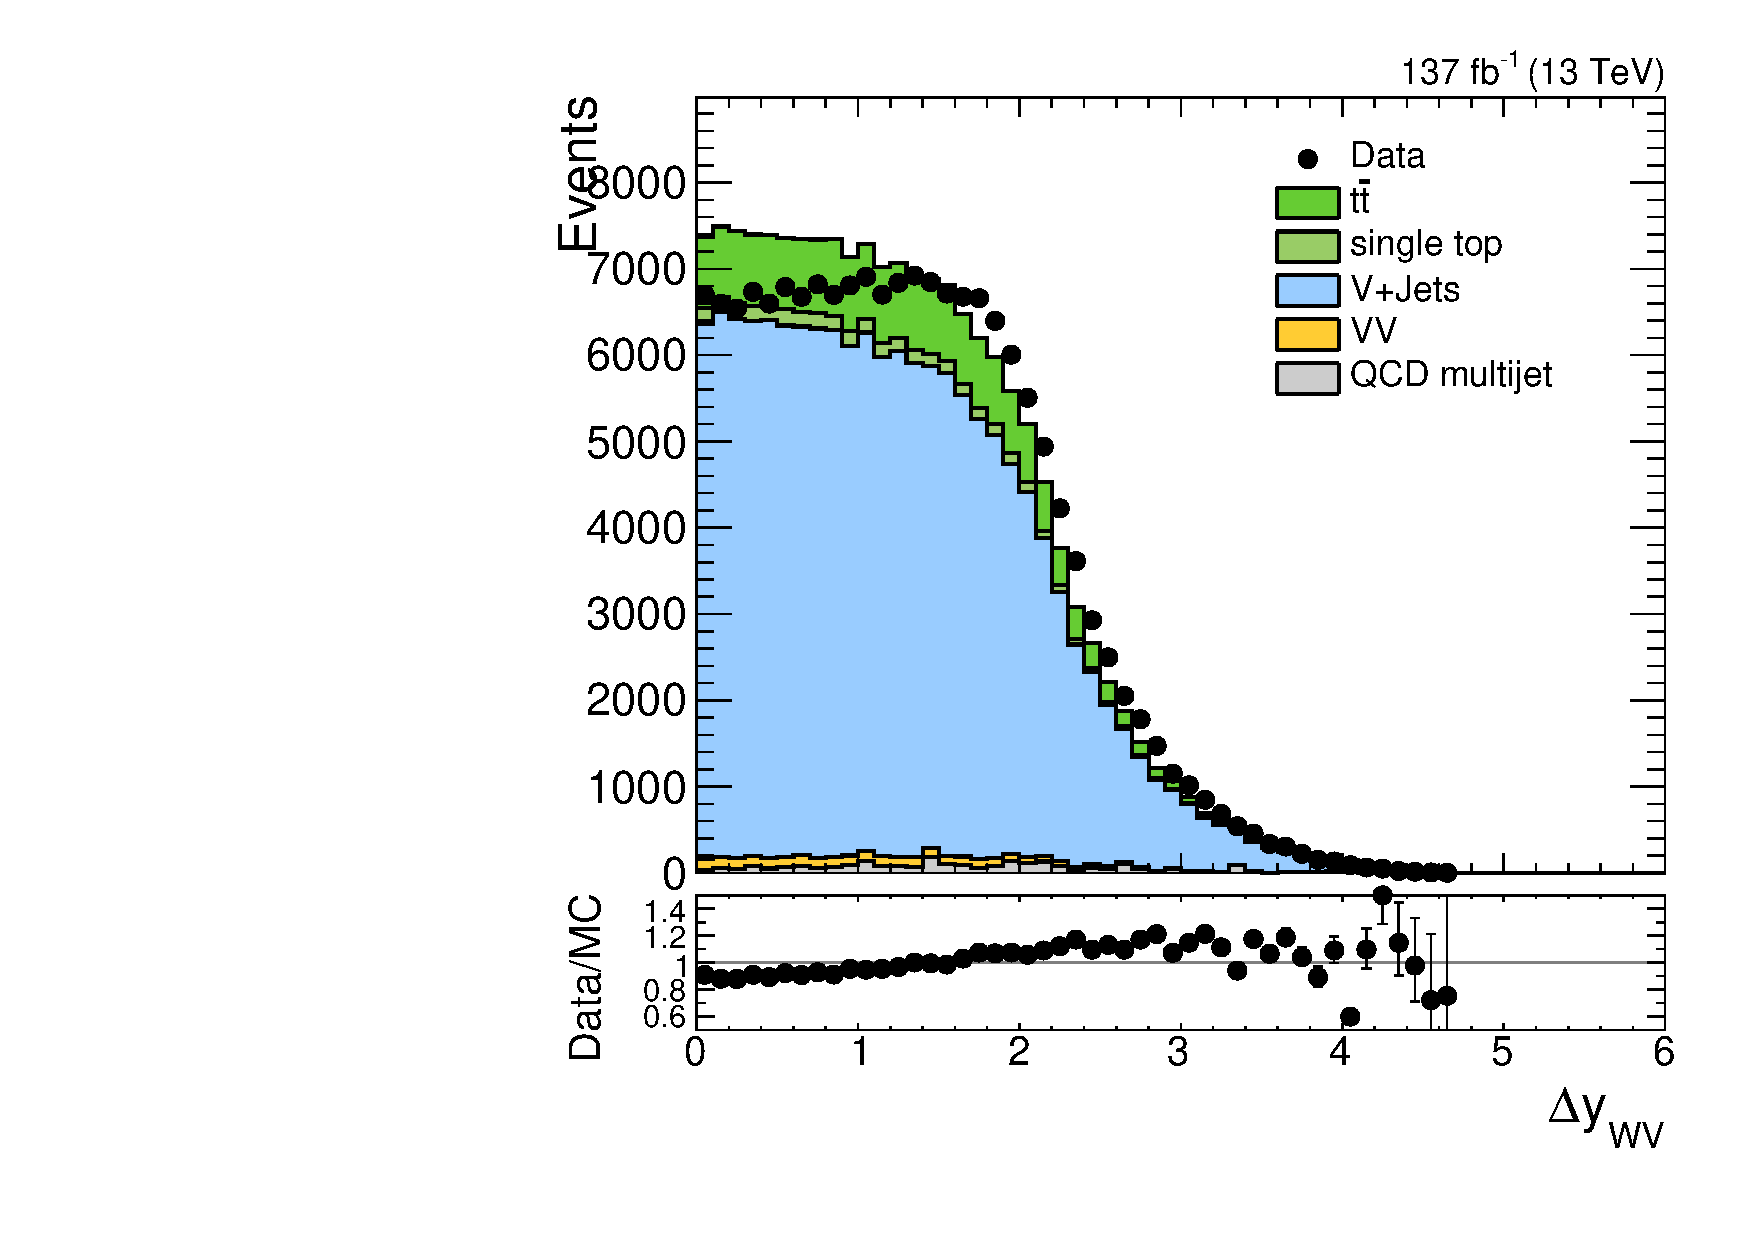
\includegraphics[width=0.3825\textwidth]{fig/analysisAppendix/SB_b1_allL_allP_allC_allD_Run2_dy.pdf}\\
  \caption{
    Comparison plots between data and MC from Run 2 for the separation in $\eta$ of the \VBF forward jets, invariant mass of the \VBF jets, number of selected standard jets, and rapidity separation between the reconstructed bosons, in the jet mass sideband.
  }
  \label{fig:SB_controlPlotsRun2_4}
\end{figure}

\subsubsection{Control Plots in the Top-Enriched Control Region}

\begin{figure}[htbp]
  \centering
  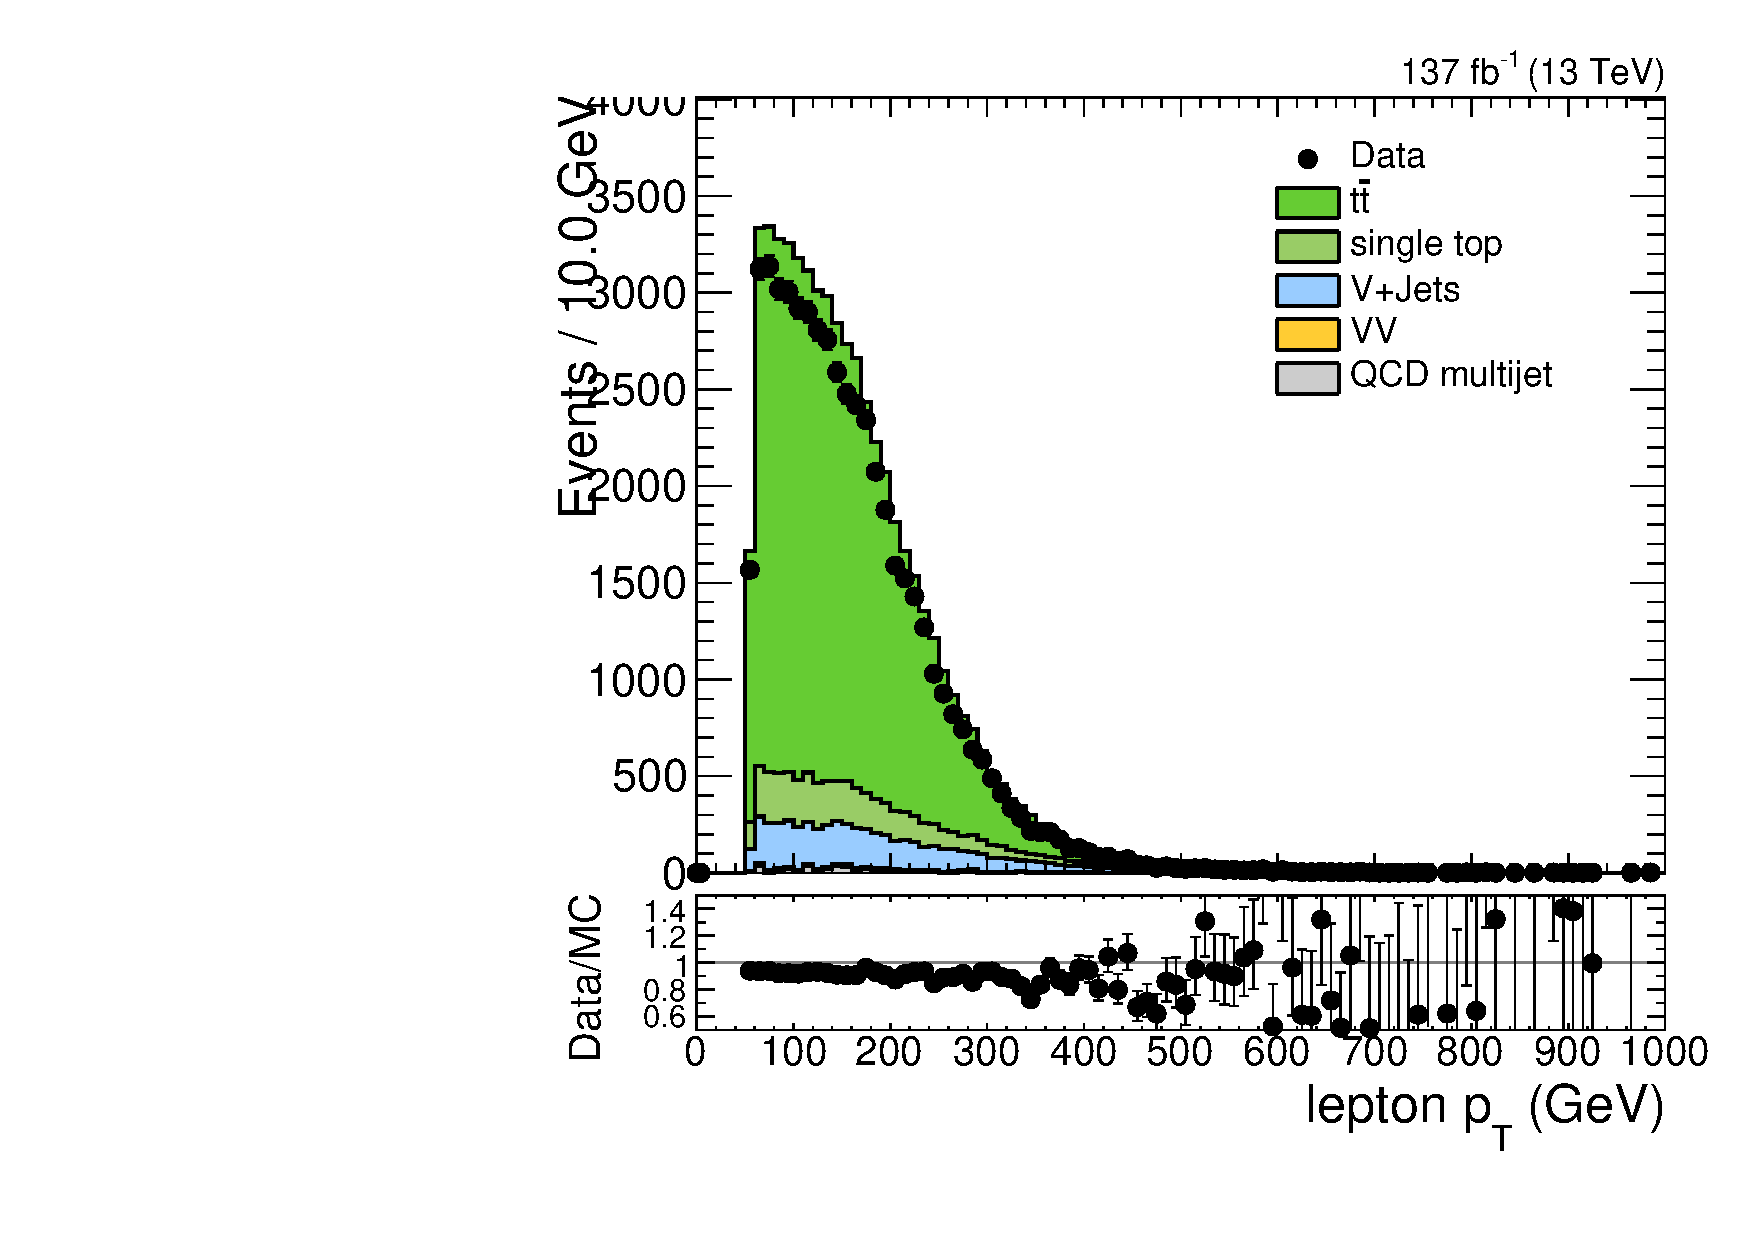
\includegraphics[width=0.3825\textwidth]{fig/analysisAppendix/CR_b1_mu_allP_allC_allD_Run2_lnujj_l1_l_pt.pdf}
  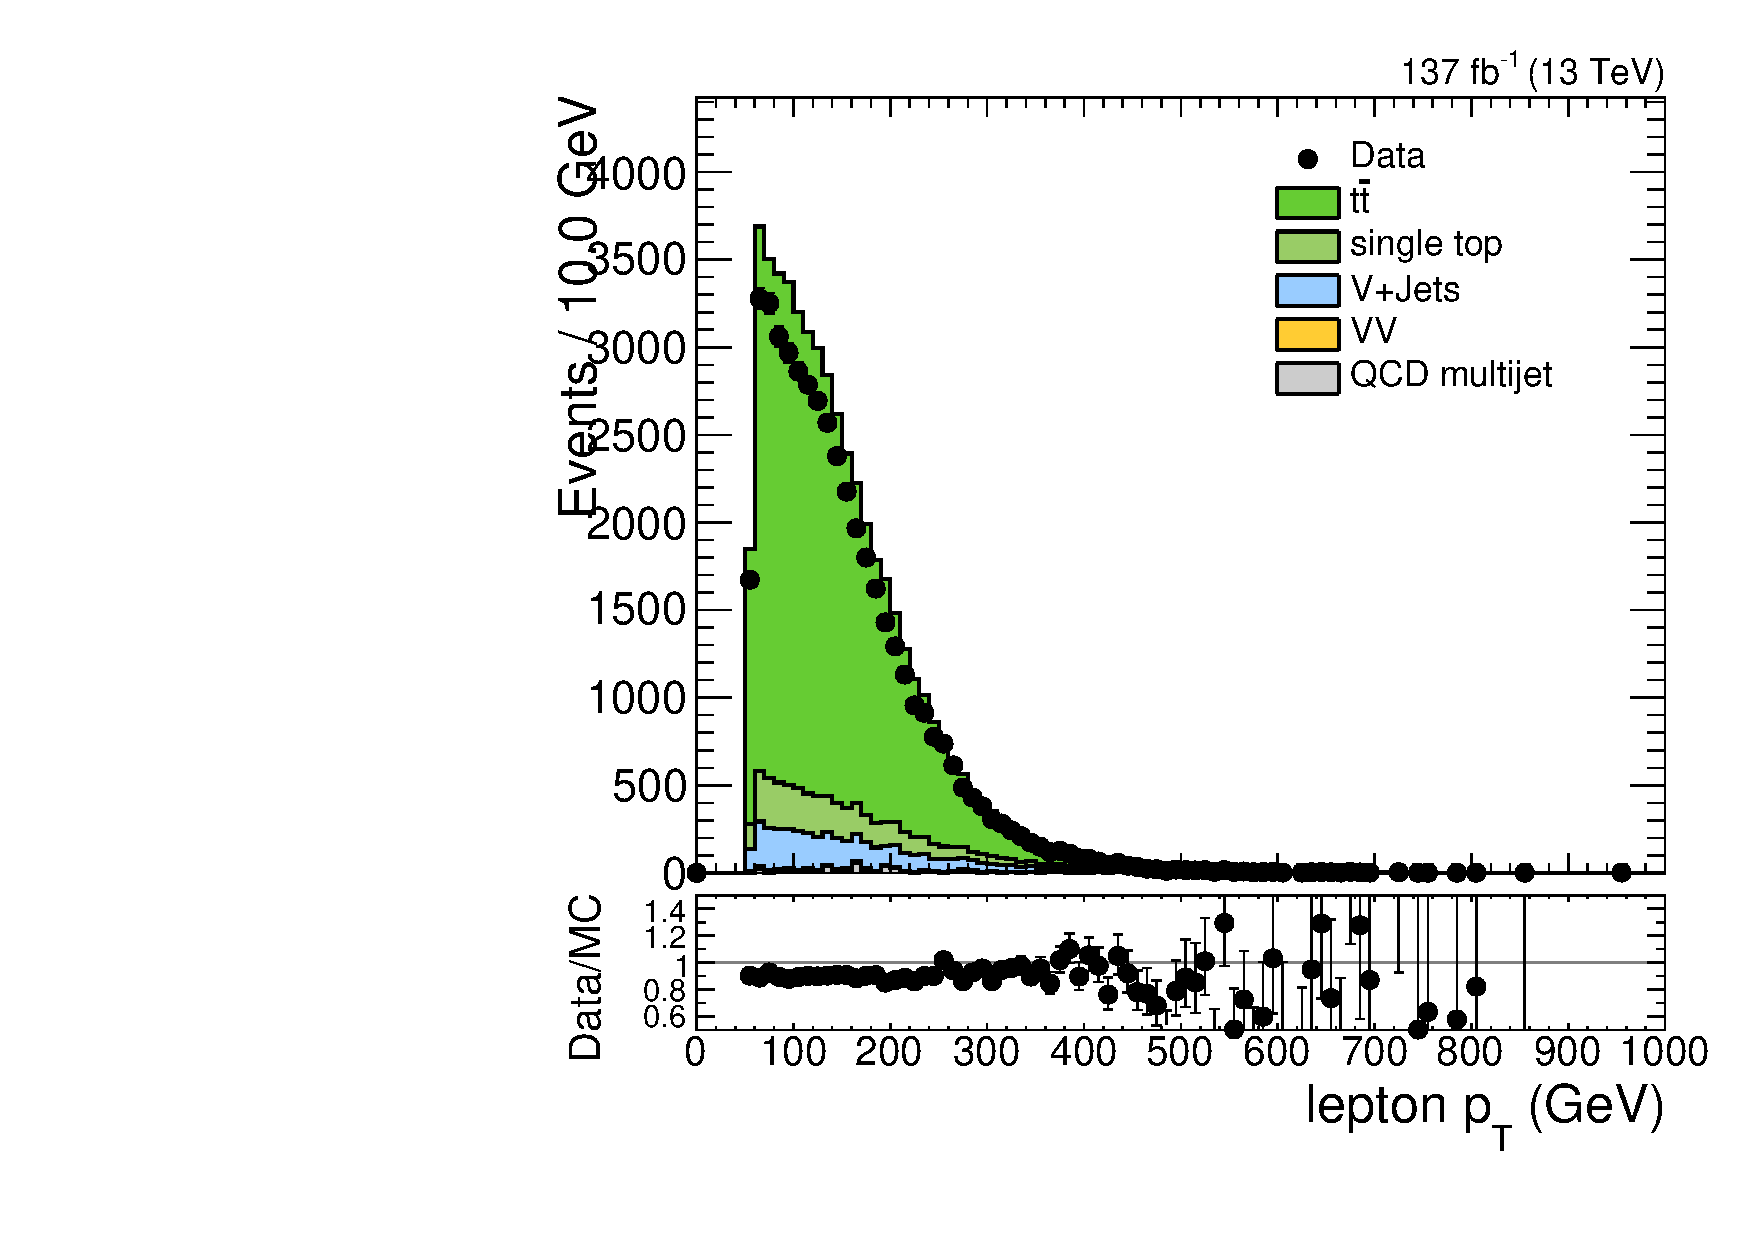
\includegraphics[width=0.3825\textwidth]{fig/analysisAppendix/CR_b1_e_allP_allC_allD_Run2_lnujj_l1_l_pt.pdf}\\
  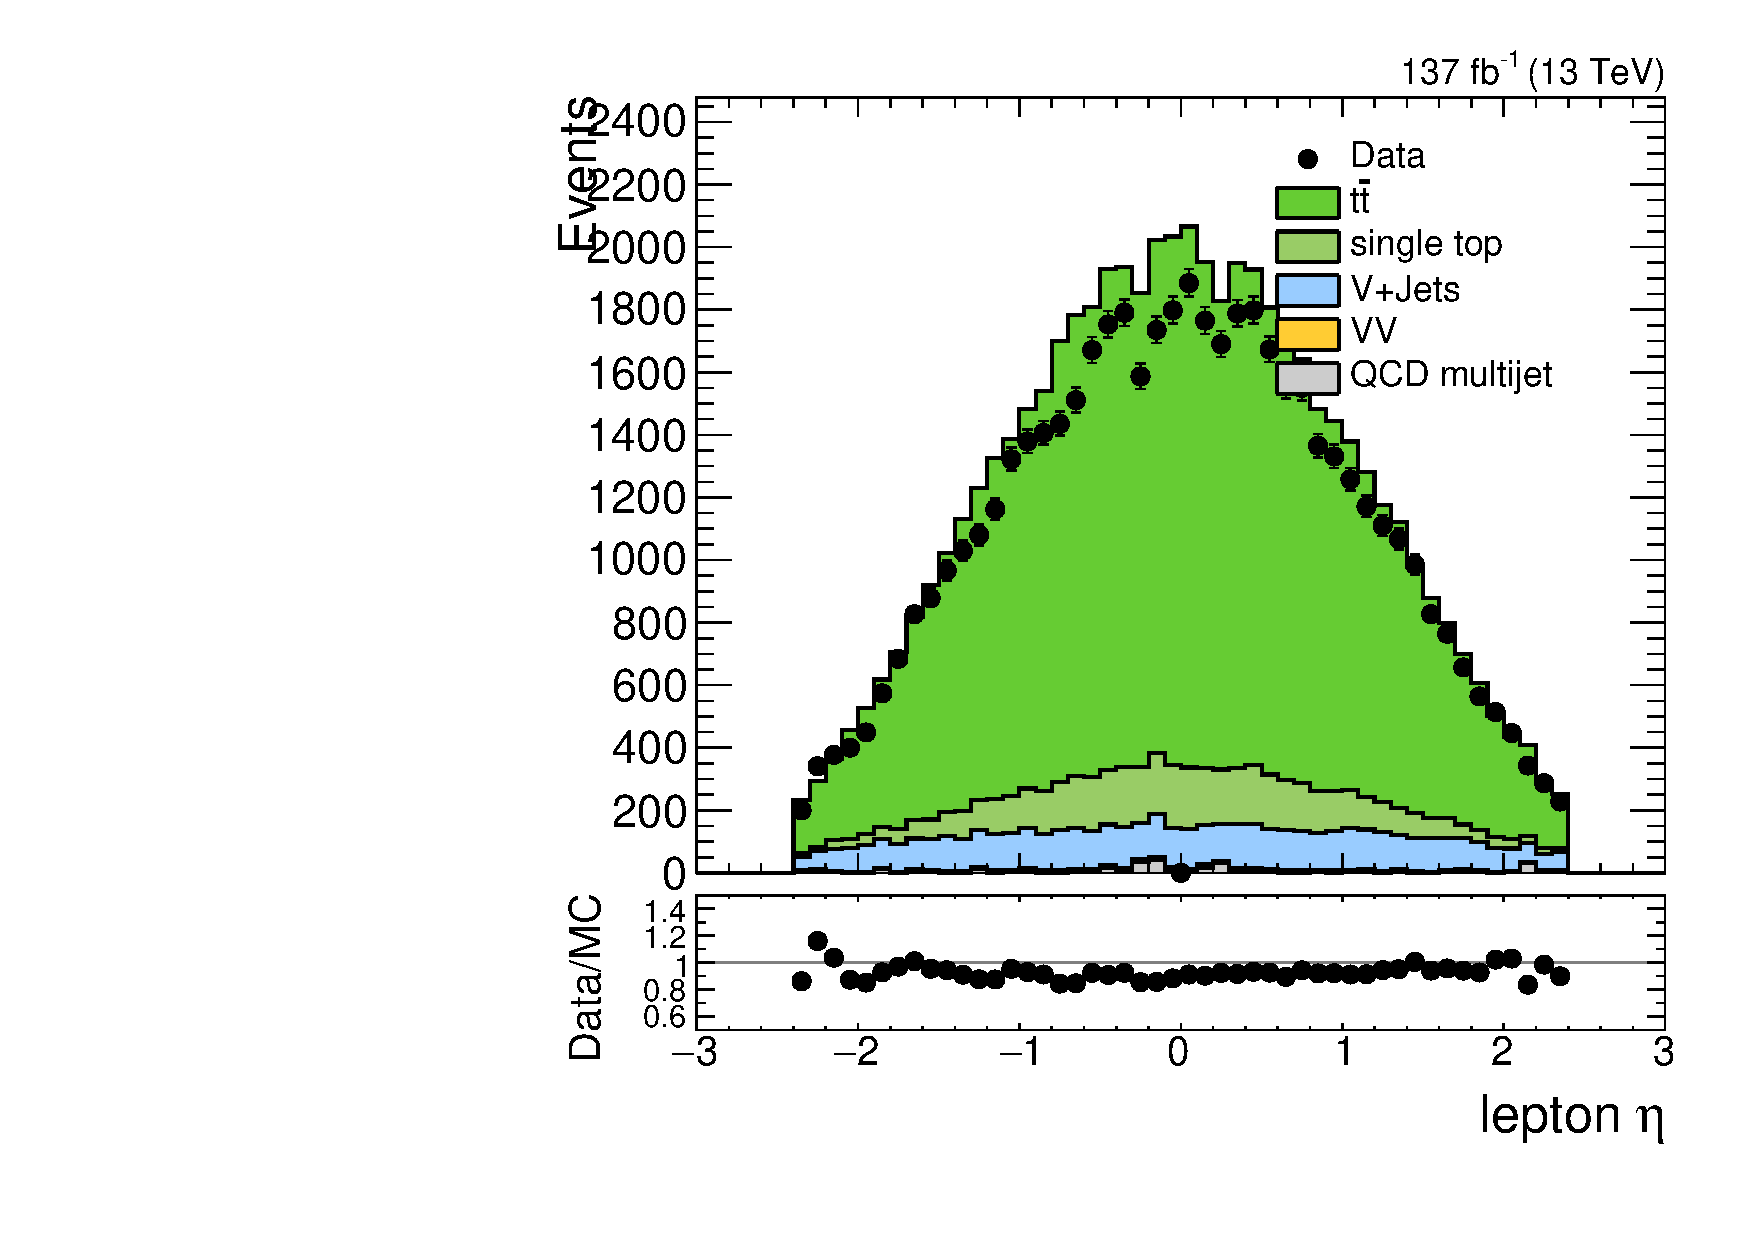
\includegraphics[width=0.3825\textwidth]{fig/analysisAppendix/CR_b1_mu_allP_allC_allD_Run2_lnujj_l1_l_eta.pdf}
  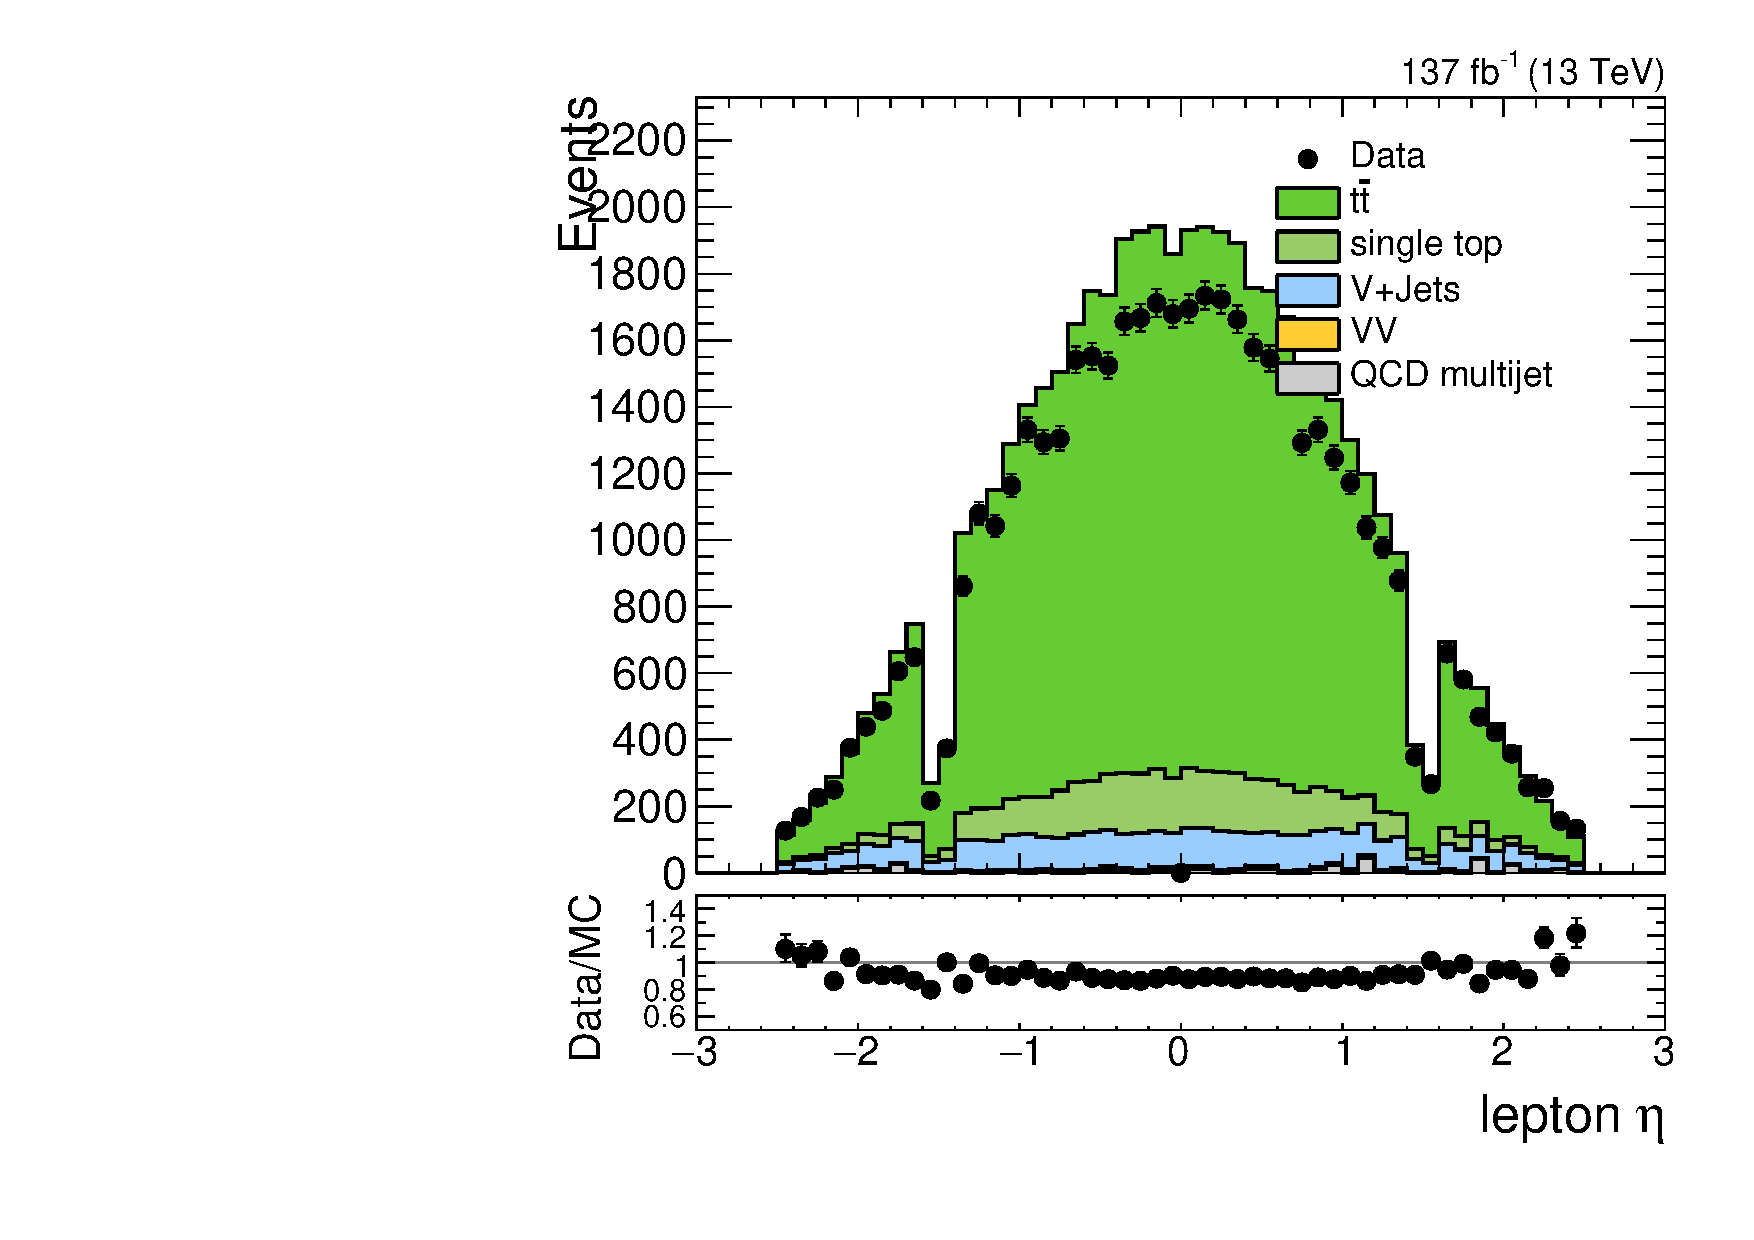
\includegraphics[width=0.3825\textwidth]{fig/analysisAppendix/CR_b1_e_allP_allC_allD_Run2_lnujj_l1_l_eta.pdf}\\
  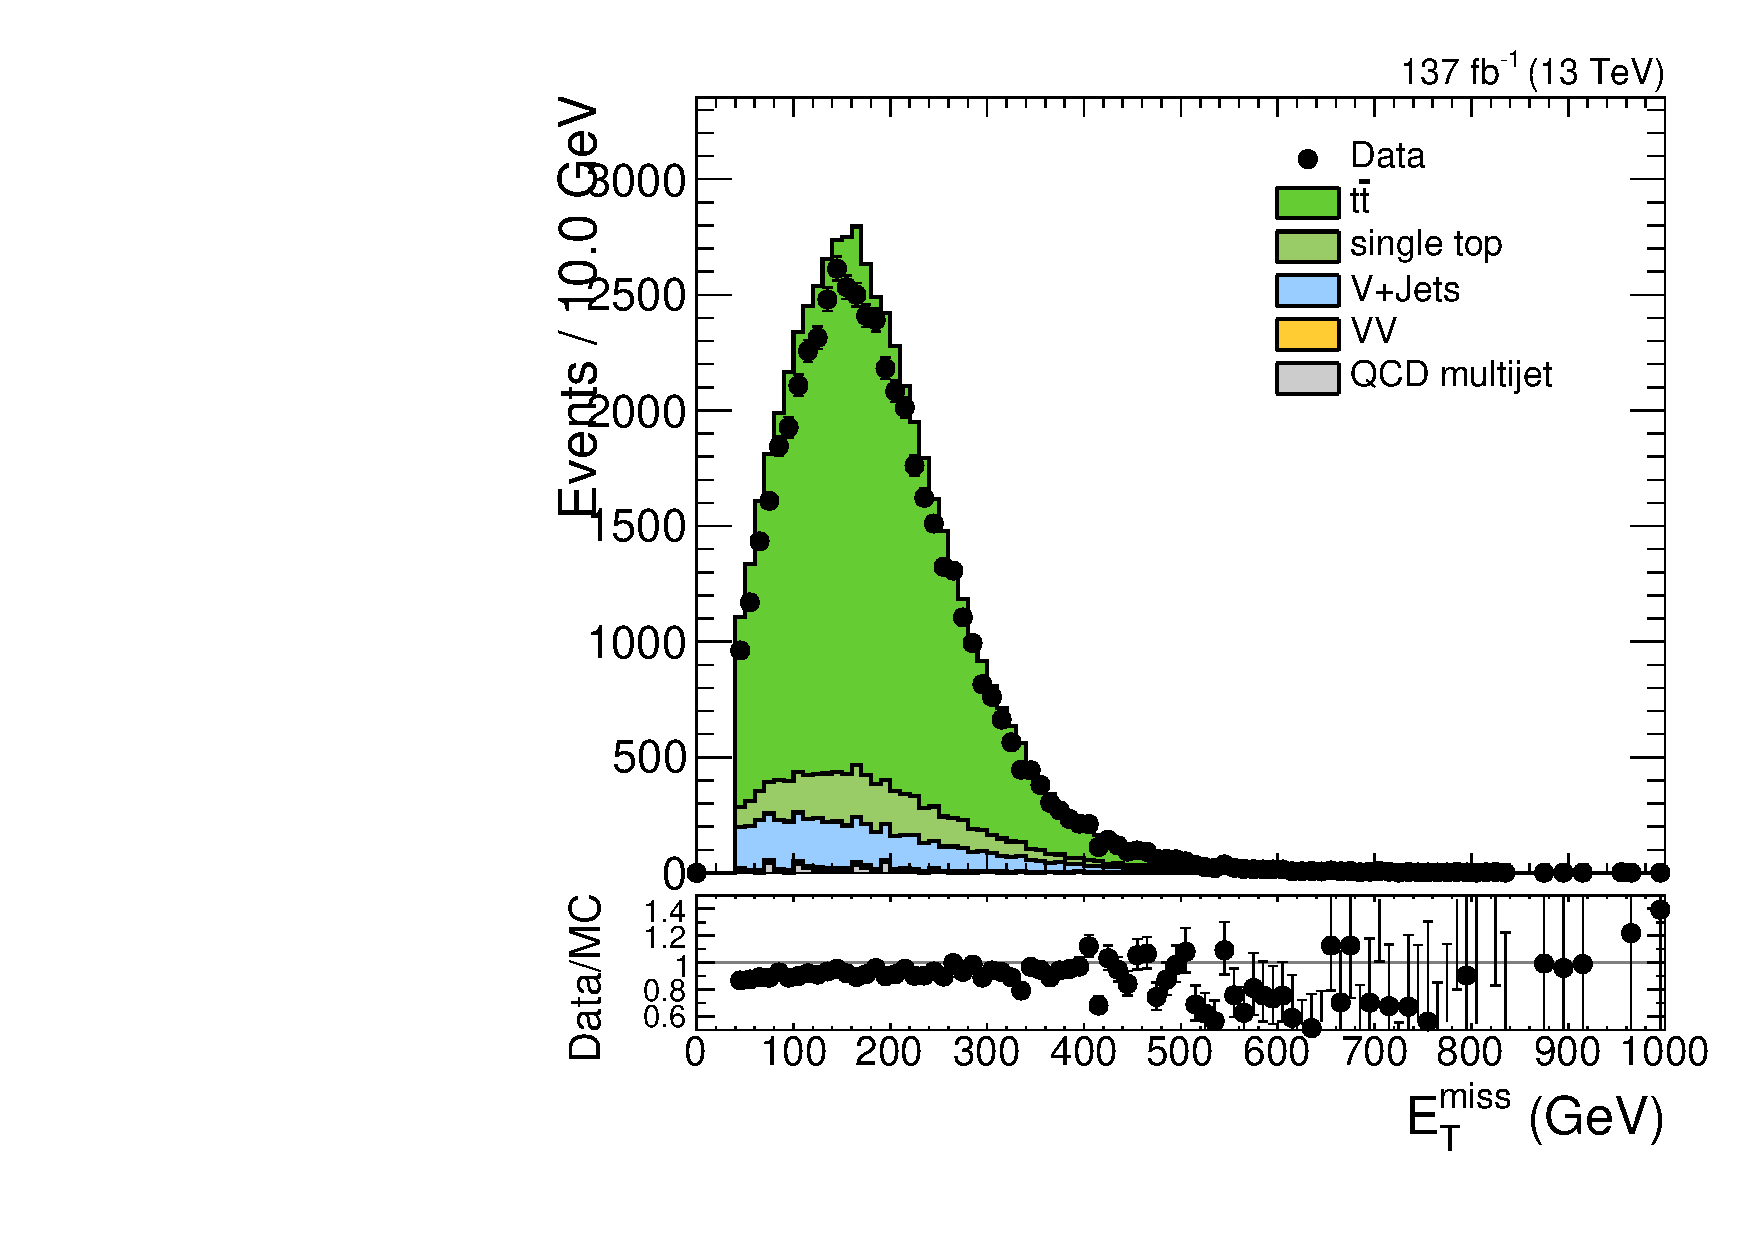
\includegraphics[width=0.3825\textwidth]{fig/analysisAppendix/CR_b1_mu_allP_allC_allD_Run2_met_pt.pdf}
  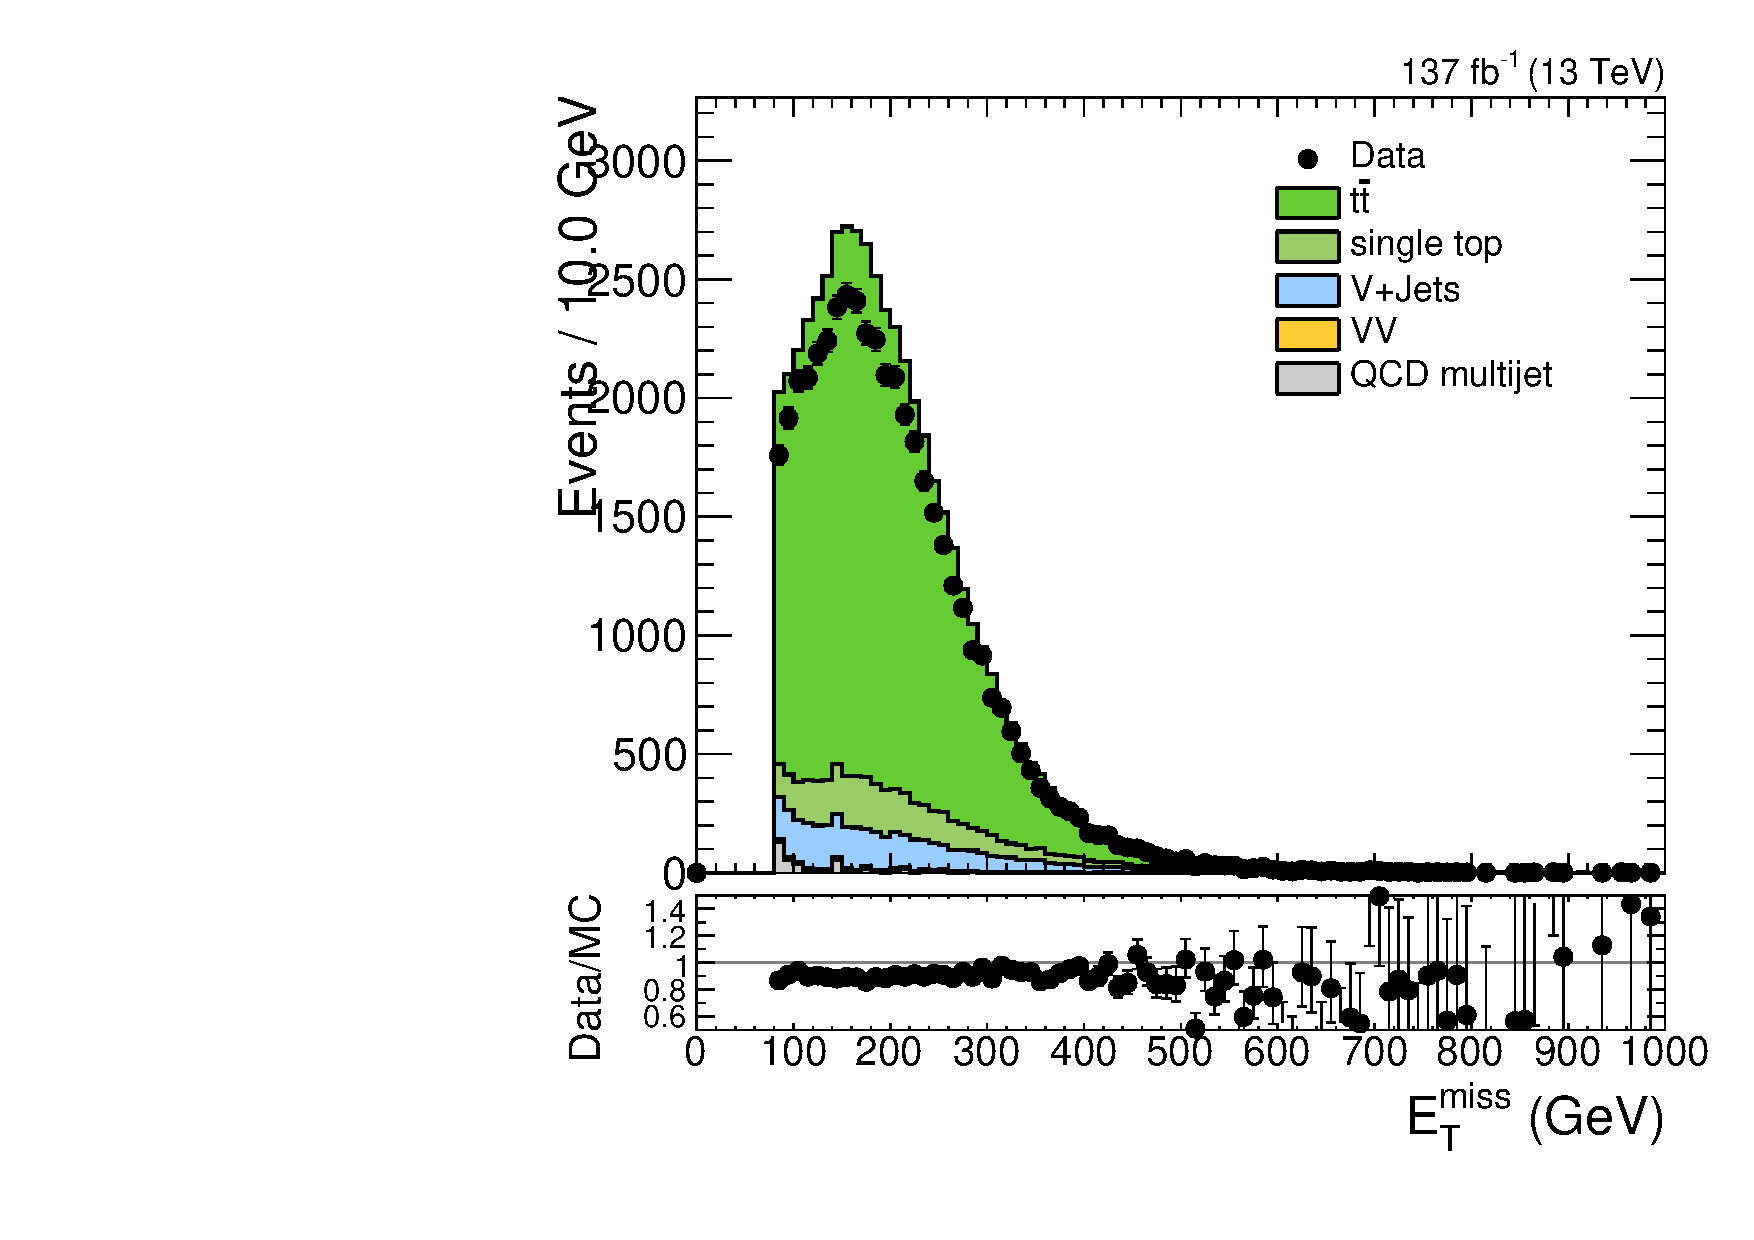
\includegraphics[width=0.3825\textwidth]{fig/analysisAppendix/CR_b1_e_allP_allC_allD_Run2_met_pt.pdf}\\
  \caption{
    Comparison plots between data and MC from Run 2 for different \Wlep-related observables, in the top-enriched control region.
    From top to bottom: lepton \pt, lepton $\eta$, \ptmiss.
    Left: muon channel, right: electron channel.
  }
  \label{fig:CR_controlPlotsRun2_1}
\end{figure}

\begin{figure}[htbp]
  \centering
  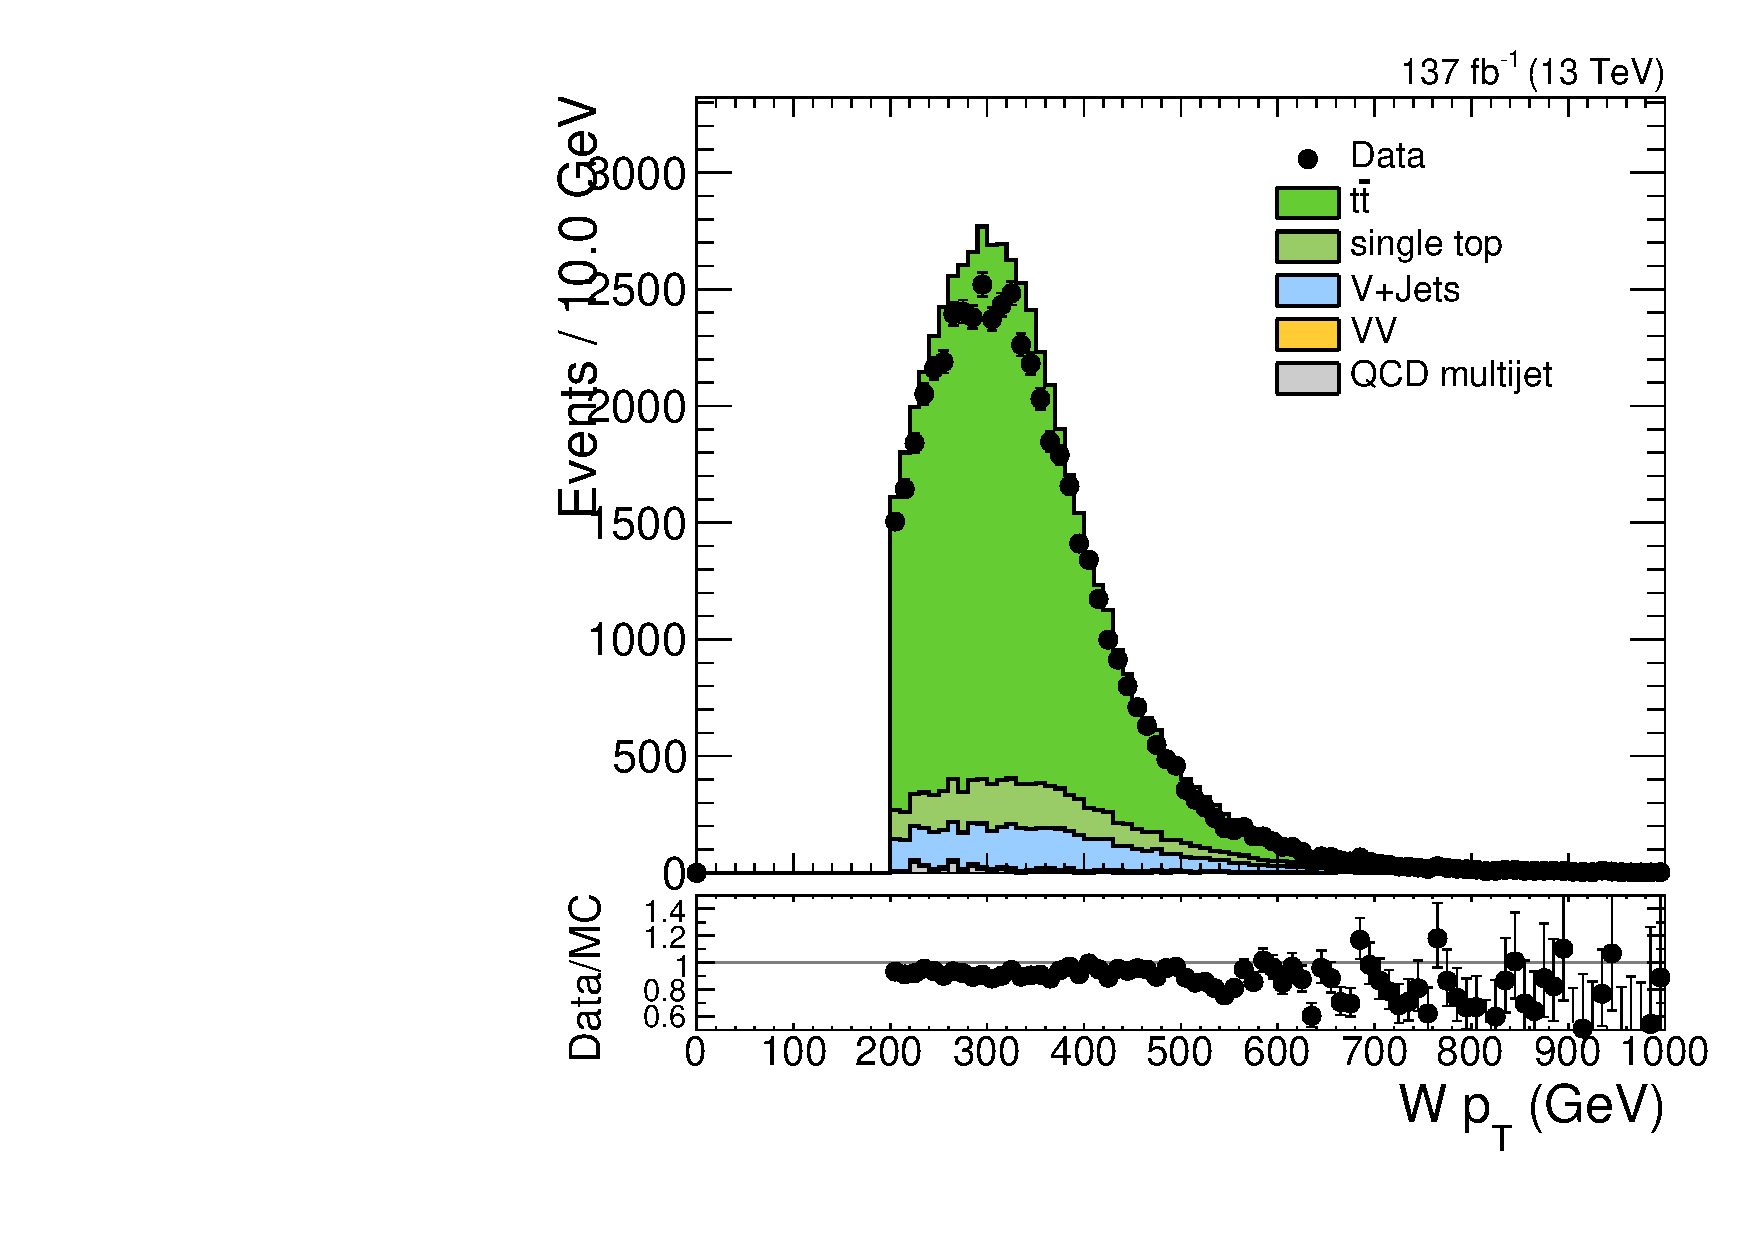
\includegraphics[width=0.3825\textwidth]{fig/analysisAppendix/CR_b1_mu_allP_allC_allD_Run2_lnujj_l1_pt.pdf}
  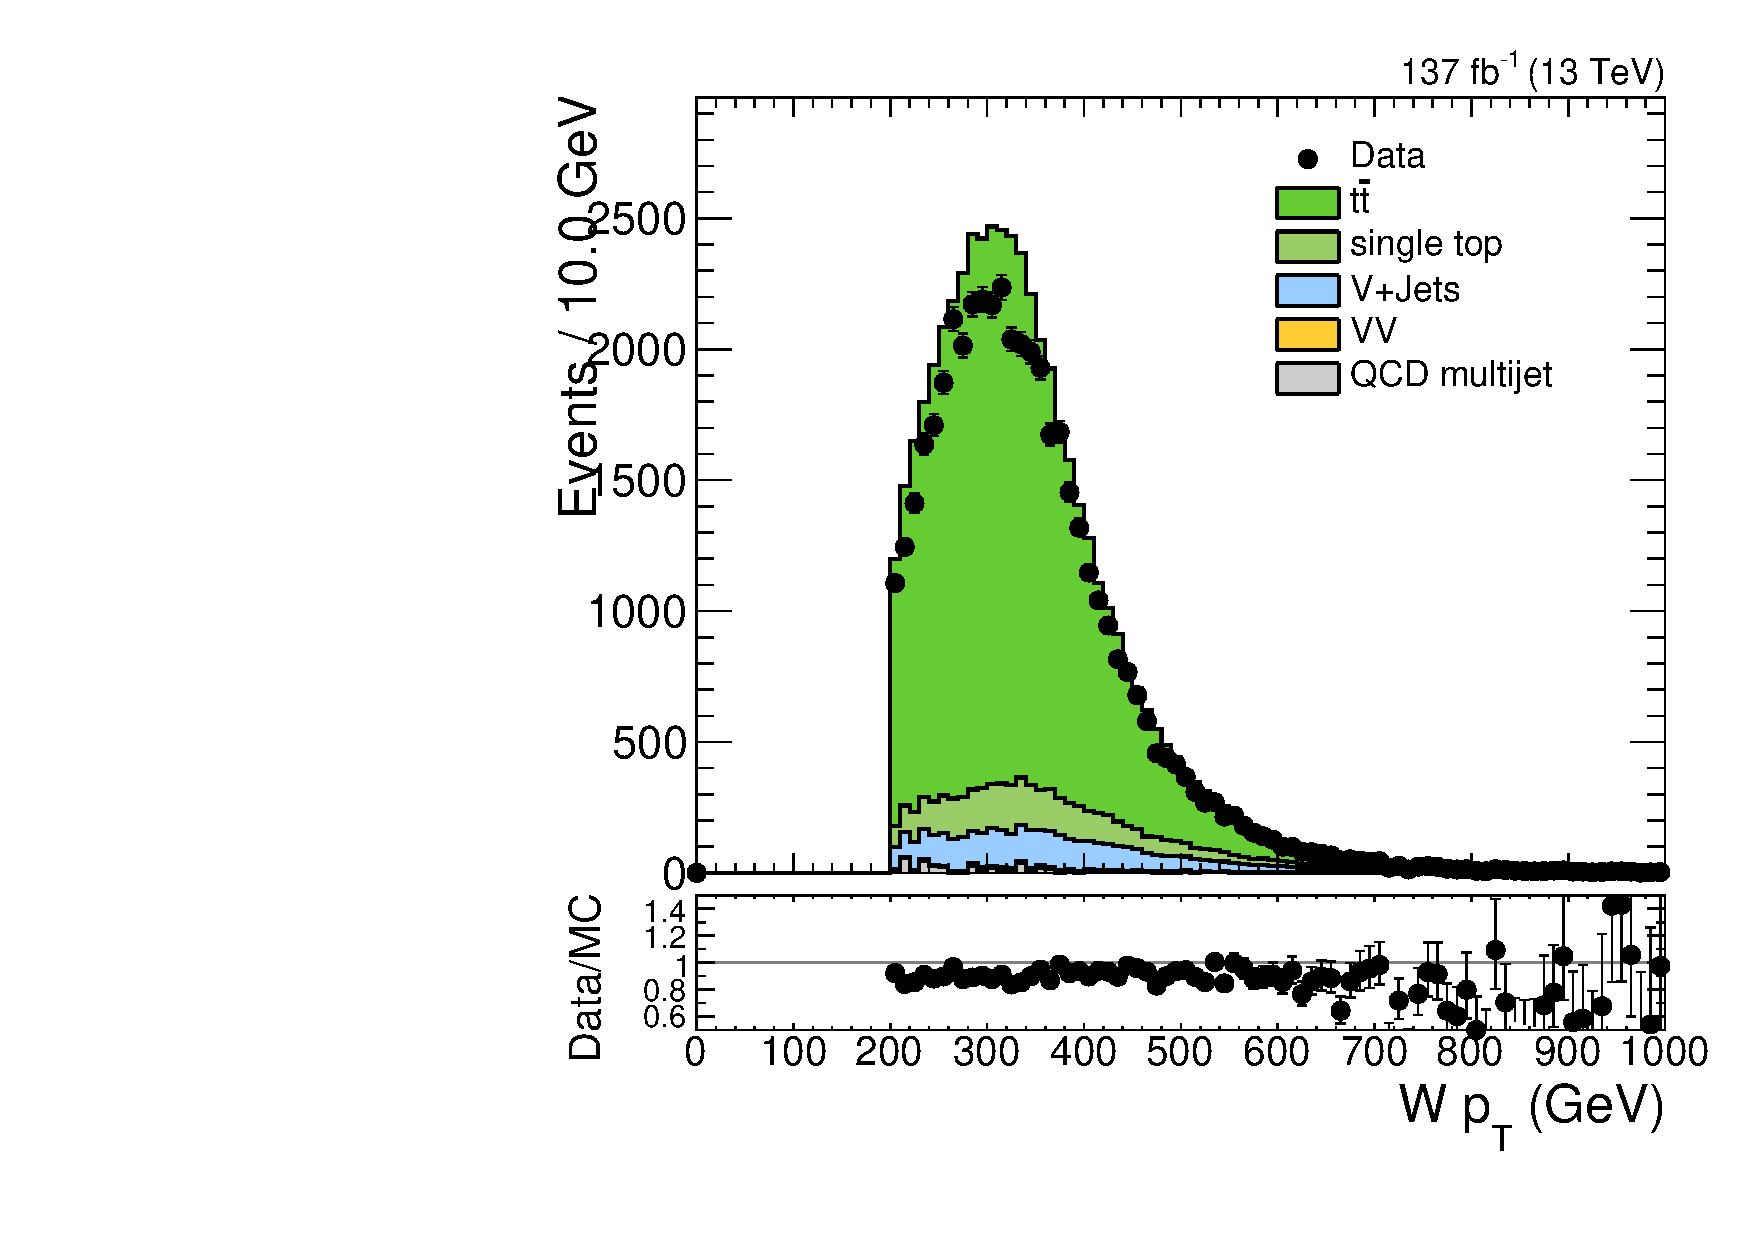
\includegraphics[width=0.3825\textwidth]{fig/analysisAppendix/CR_b1_e_allP_allC_allD_Run2_lnujj_l1_pt.pdf}\\
  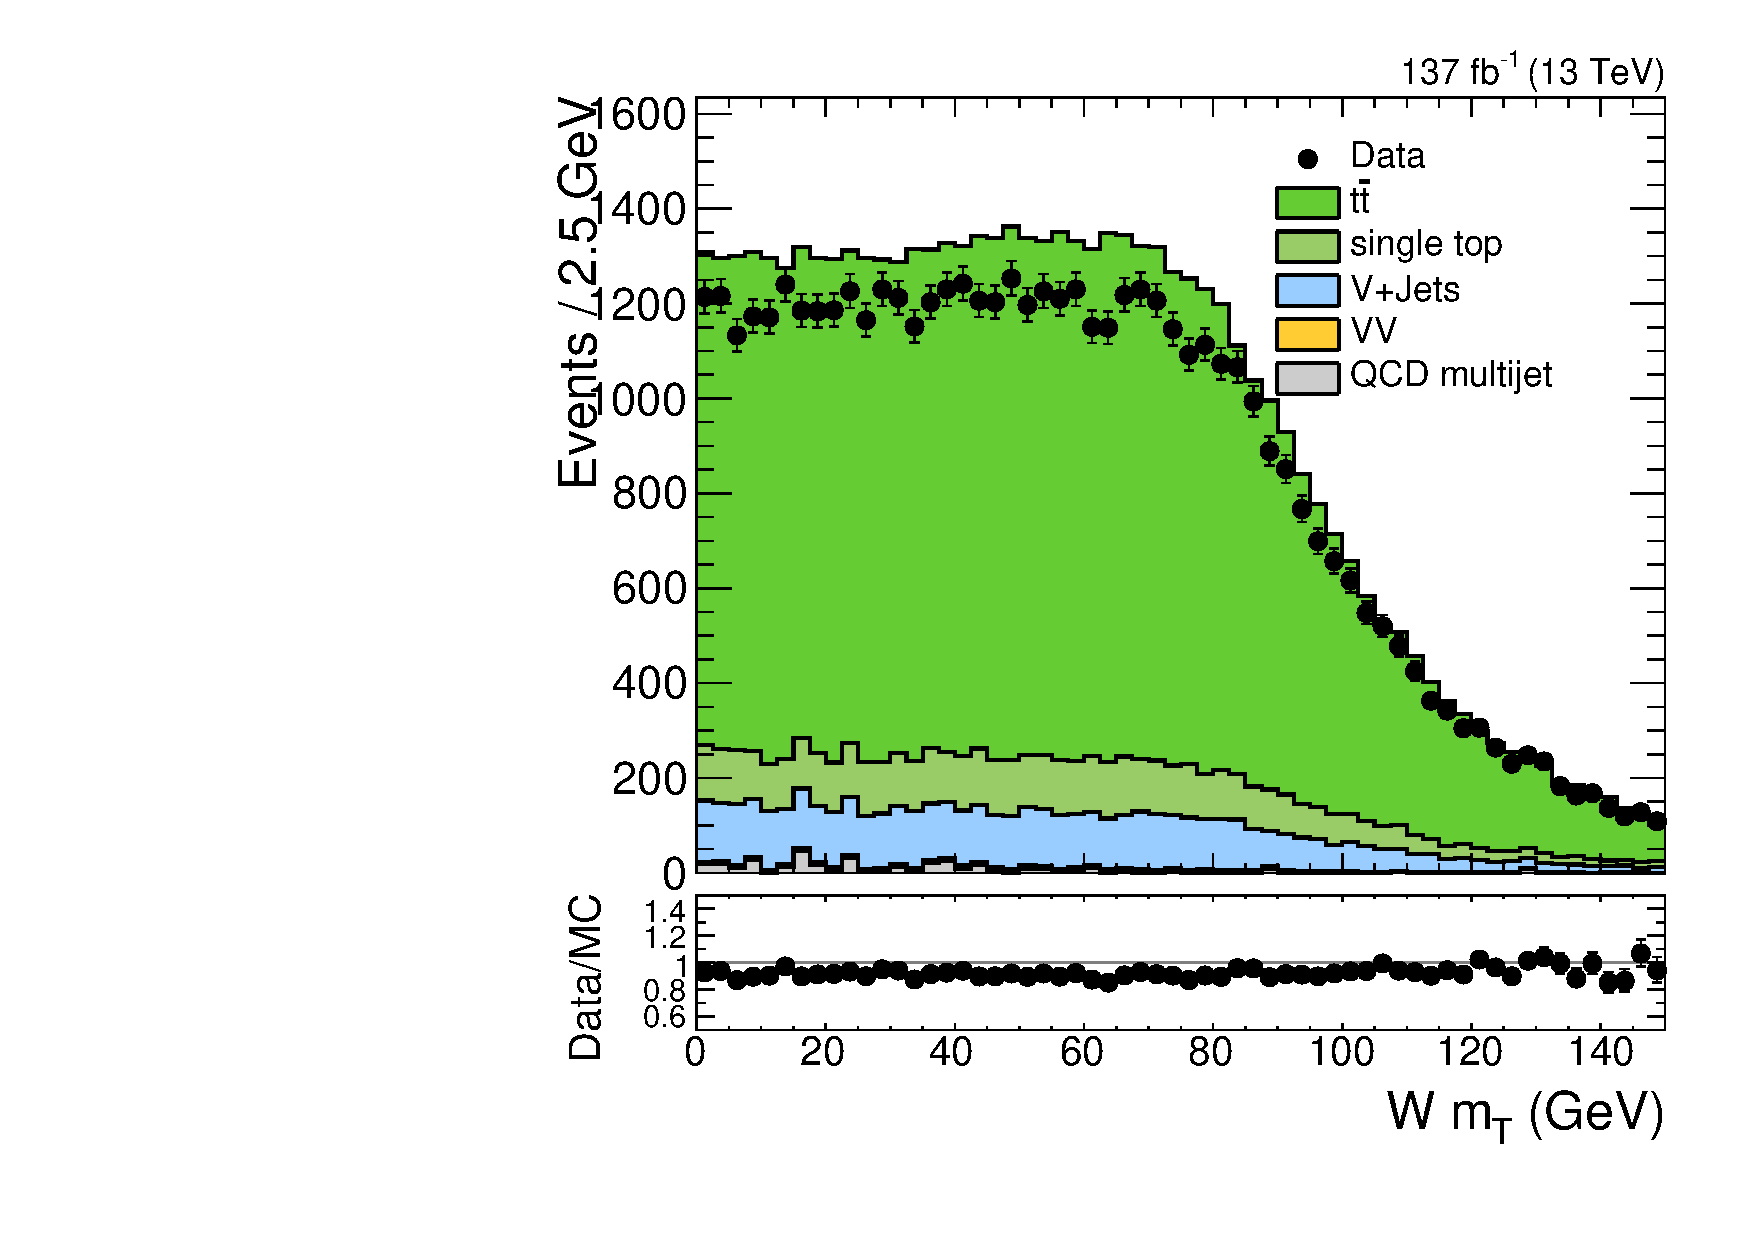
\includegraphics[width=0.3825\textwidth]{fig/analysisAppendix/CR_b1_mu_allP_allC_allD_Run2_lnujj_l1_mt.pdf}
  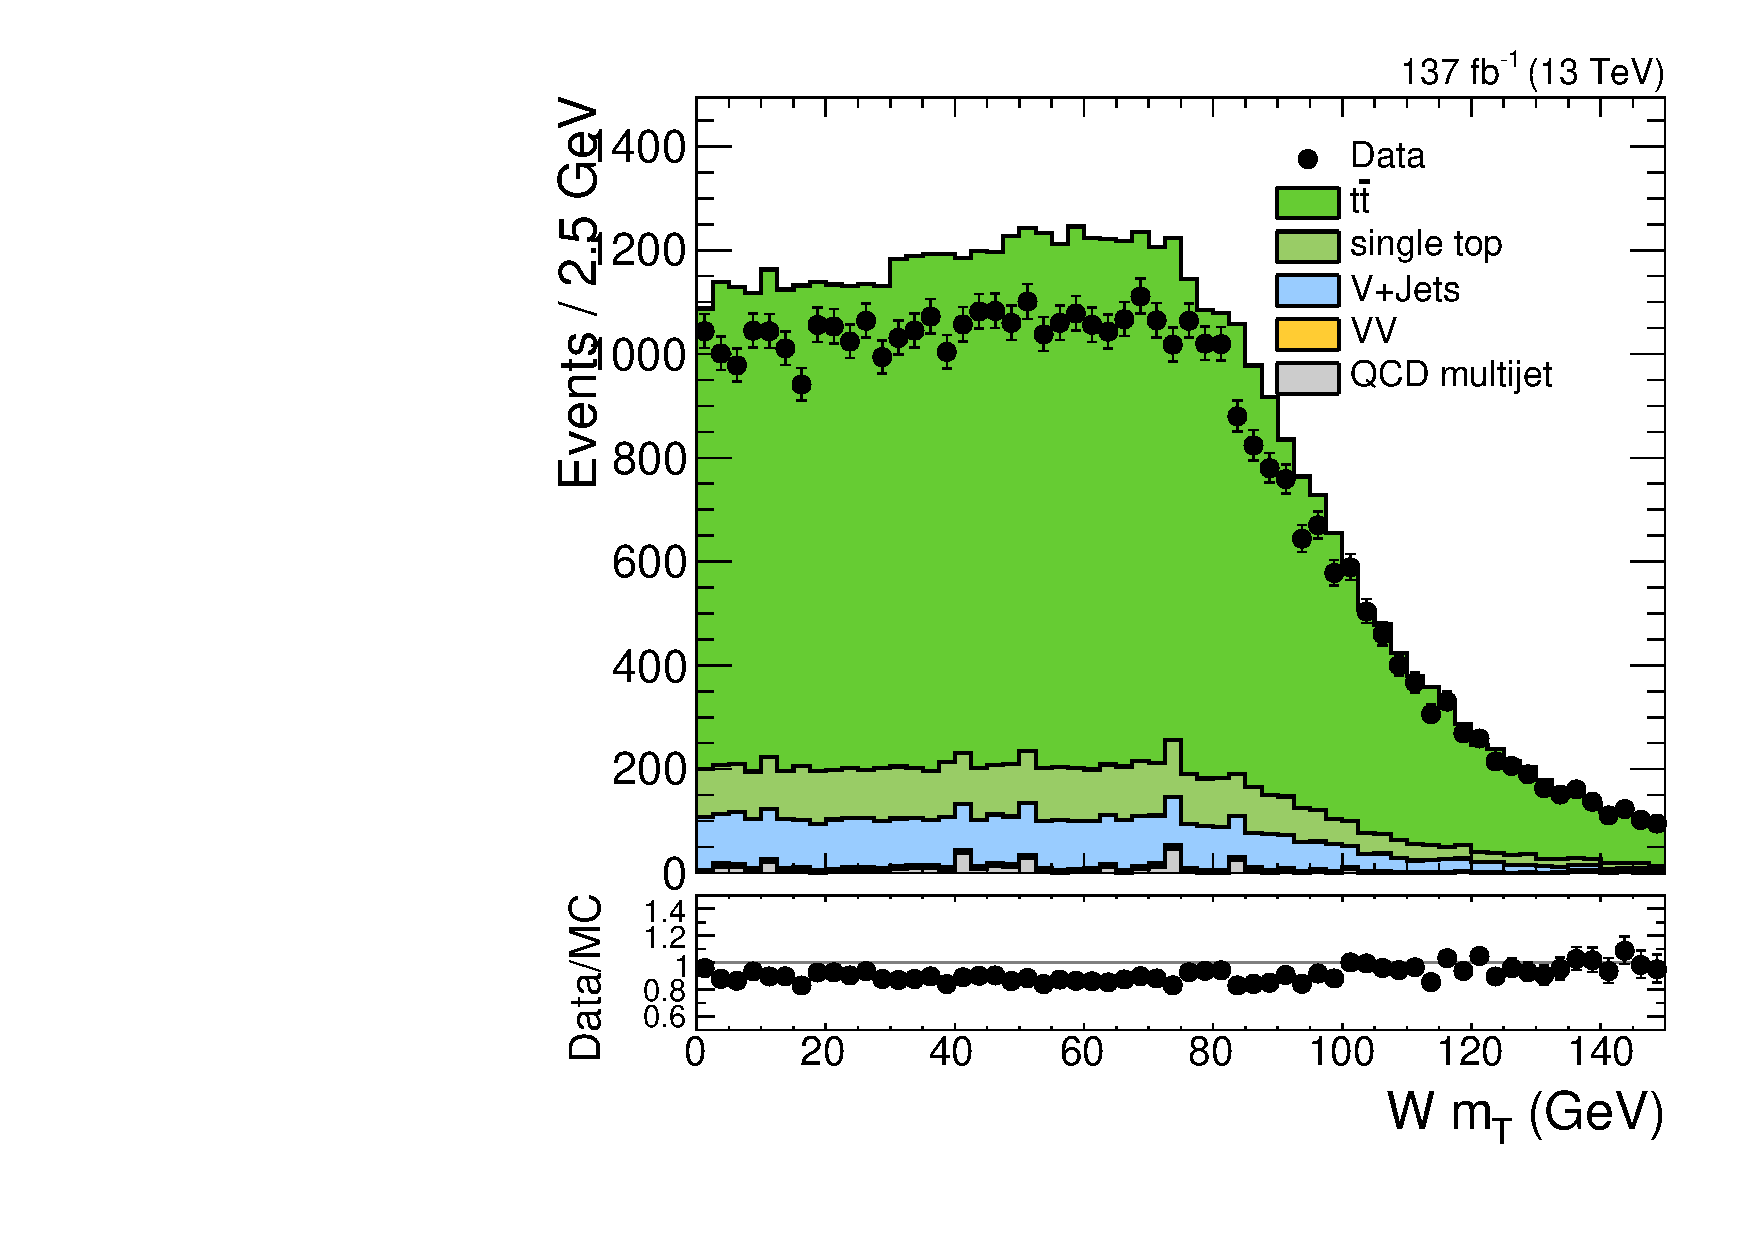
\includegraphics[width=0.3825\textwidth]{fig/analysisAppendix/CR_b1_e_allP_allC_allD_Run2_lnujj_l1_mt.pdf}\\
  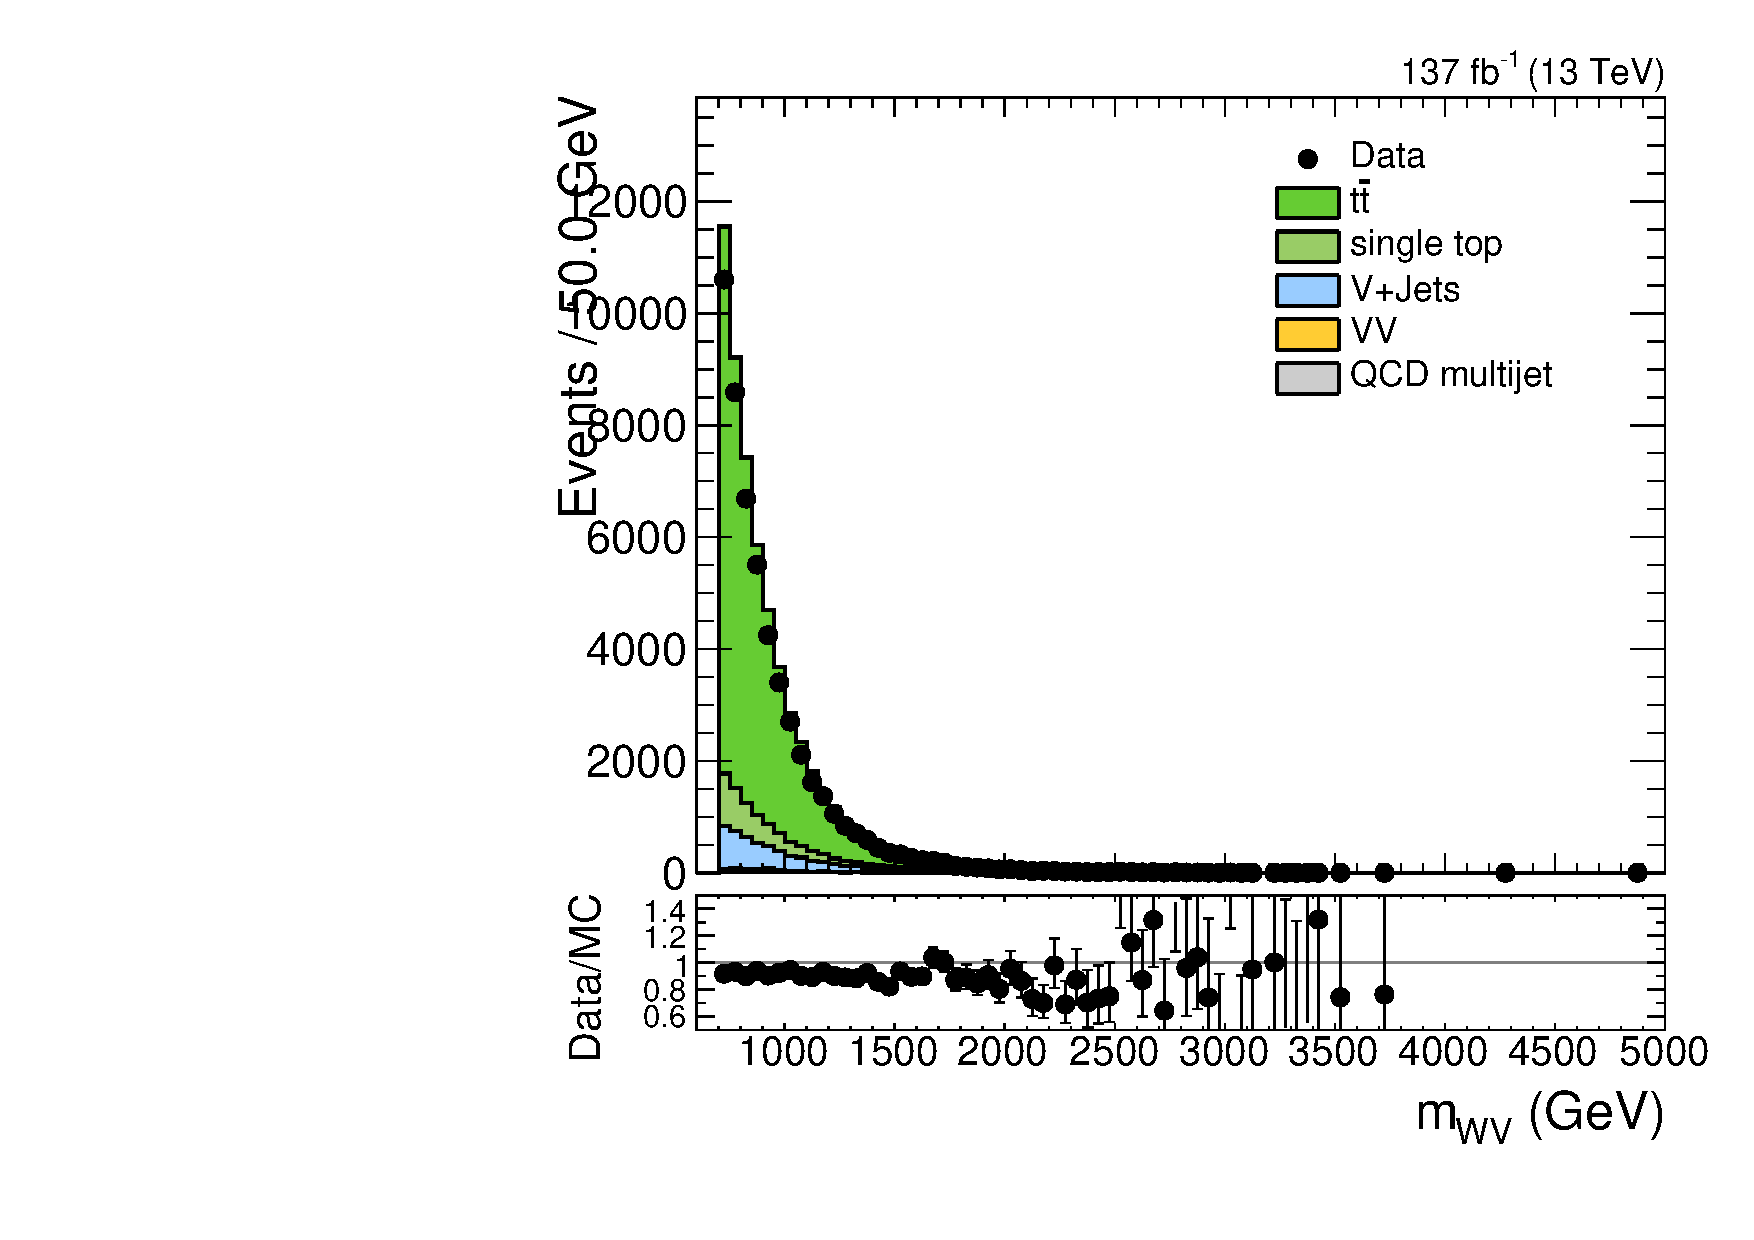
\includegraphics[width=0.3825\textwidth]{fig/analysisAppendix/CR_b1_mu_allP_allC_allD_Run2_mWV.pdf}
  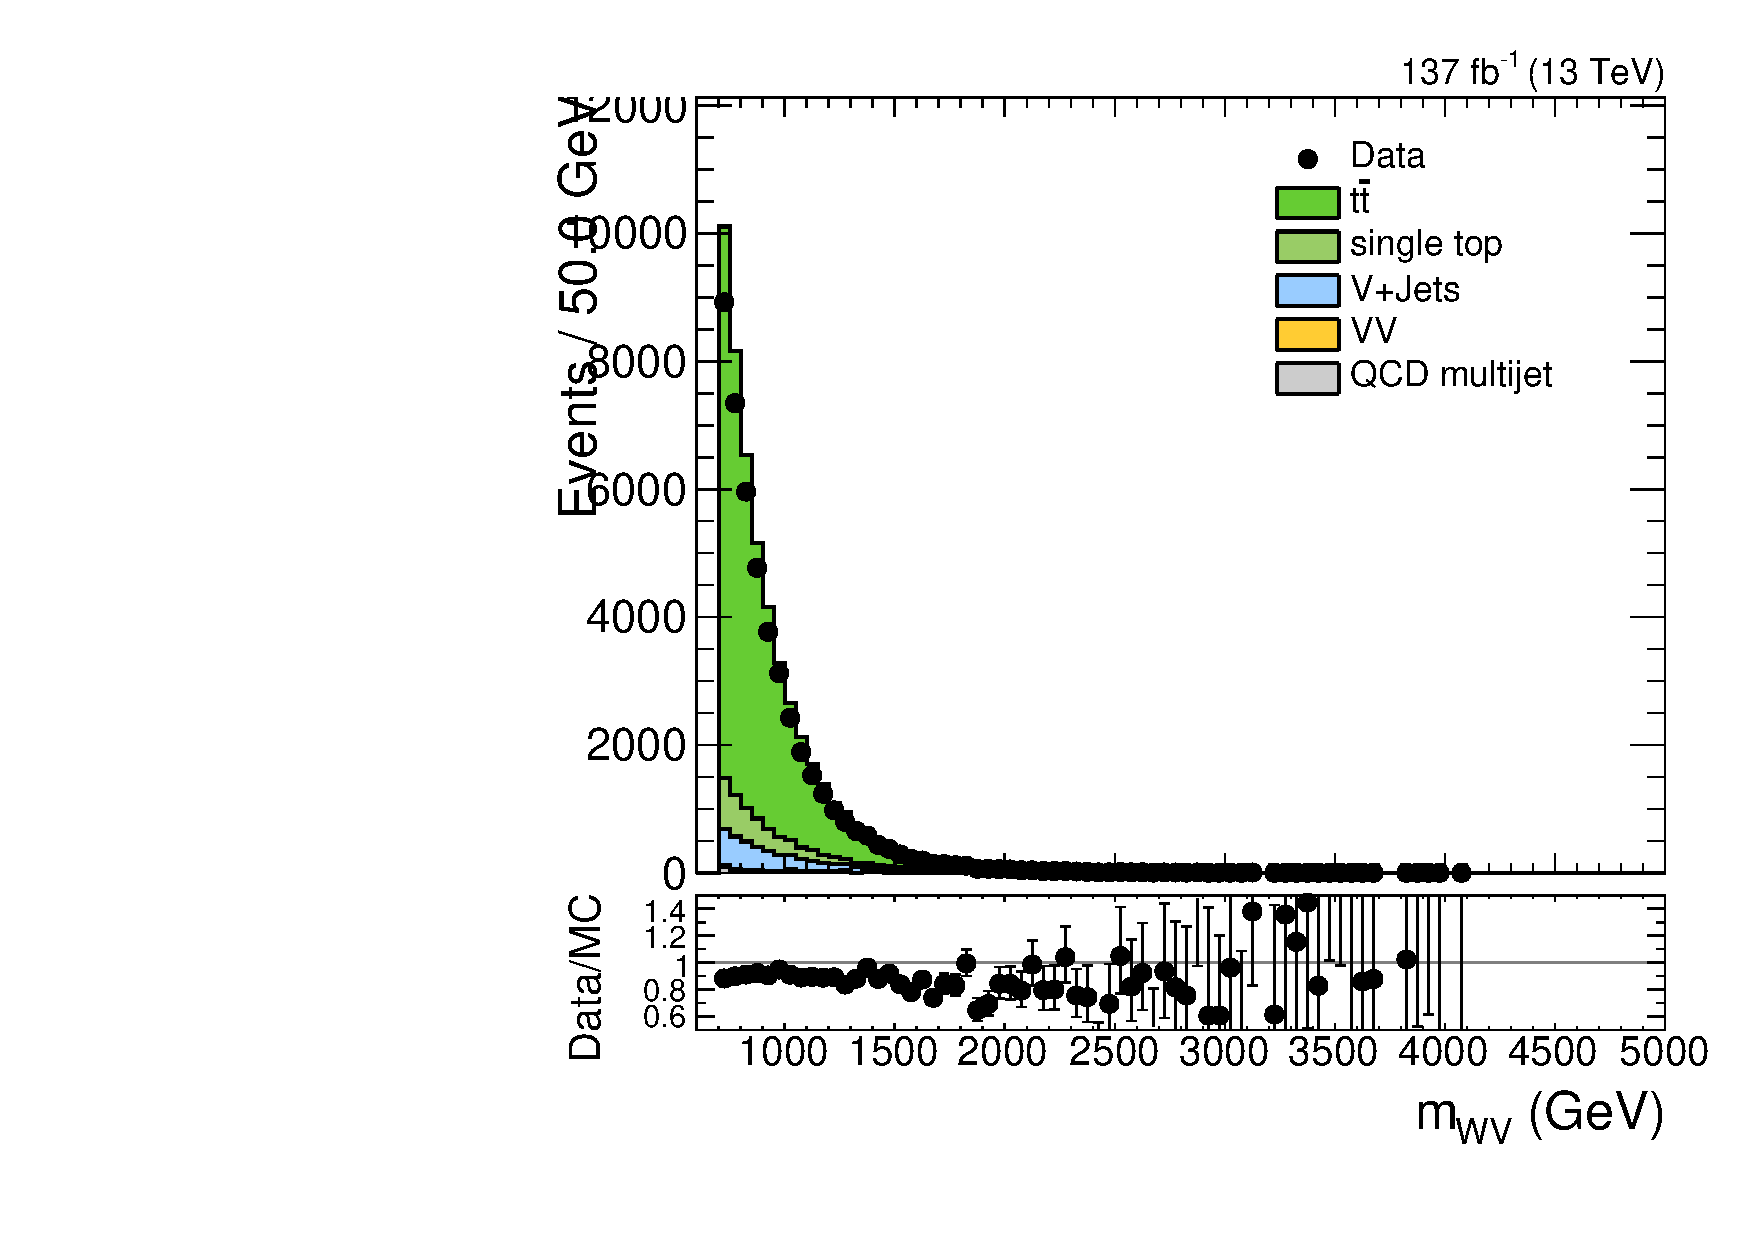
\includegraphics[width=0.3825\textwidth]{fig/analysisAppendix/CR_b1_e_allP_allC_allD_Run2_mWV.pdf}\\
  \caption{
    Comparison plots between data and MC from Run 2 for different \Wlep-related observables, in the top-enriched control region.
    From top to bottom: \pt of the leptonic $W$, transverse mass of the leptonic $W$, diboson invariant mass.
    Left: muon channel, right: electron channel.
  }
  \label{fig:CR_controlPlotsRun2_2}
\end{figure}

\begin{figure}[htbp]
  \centering
  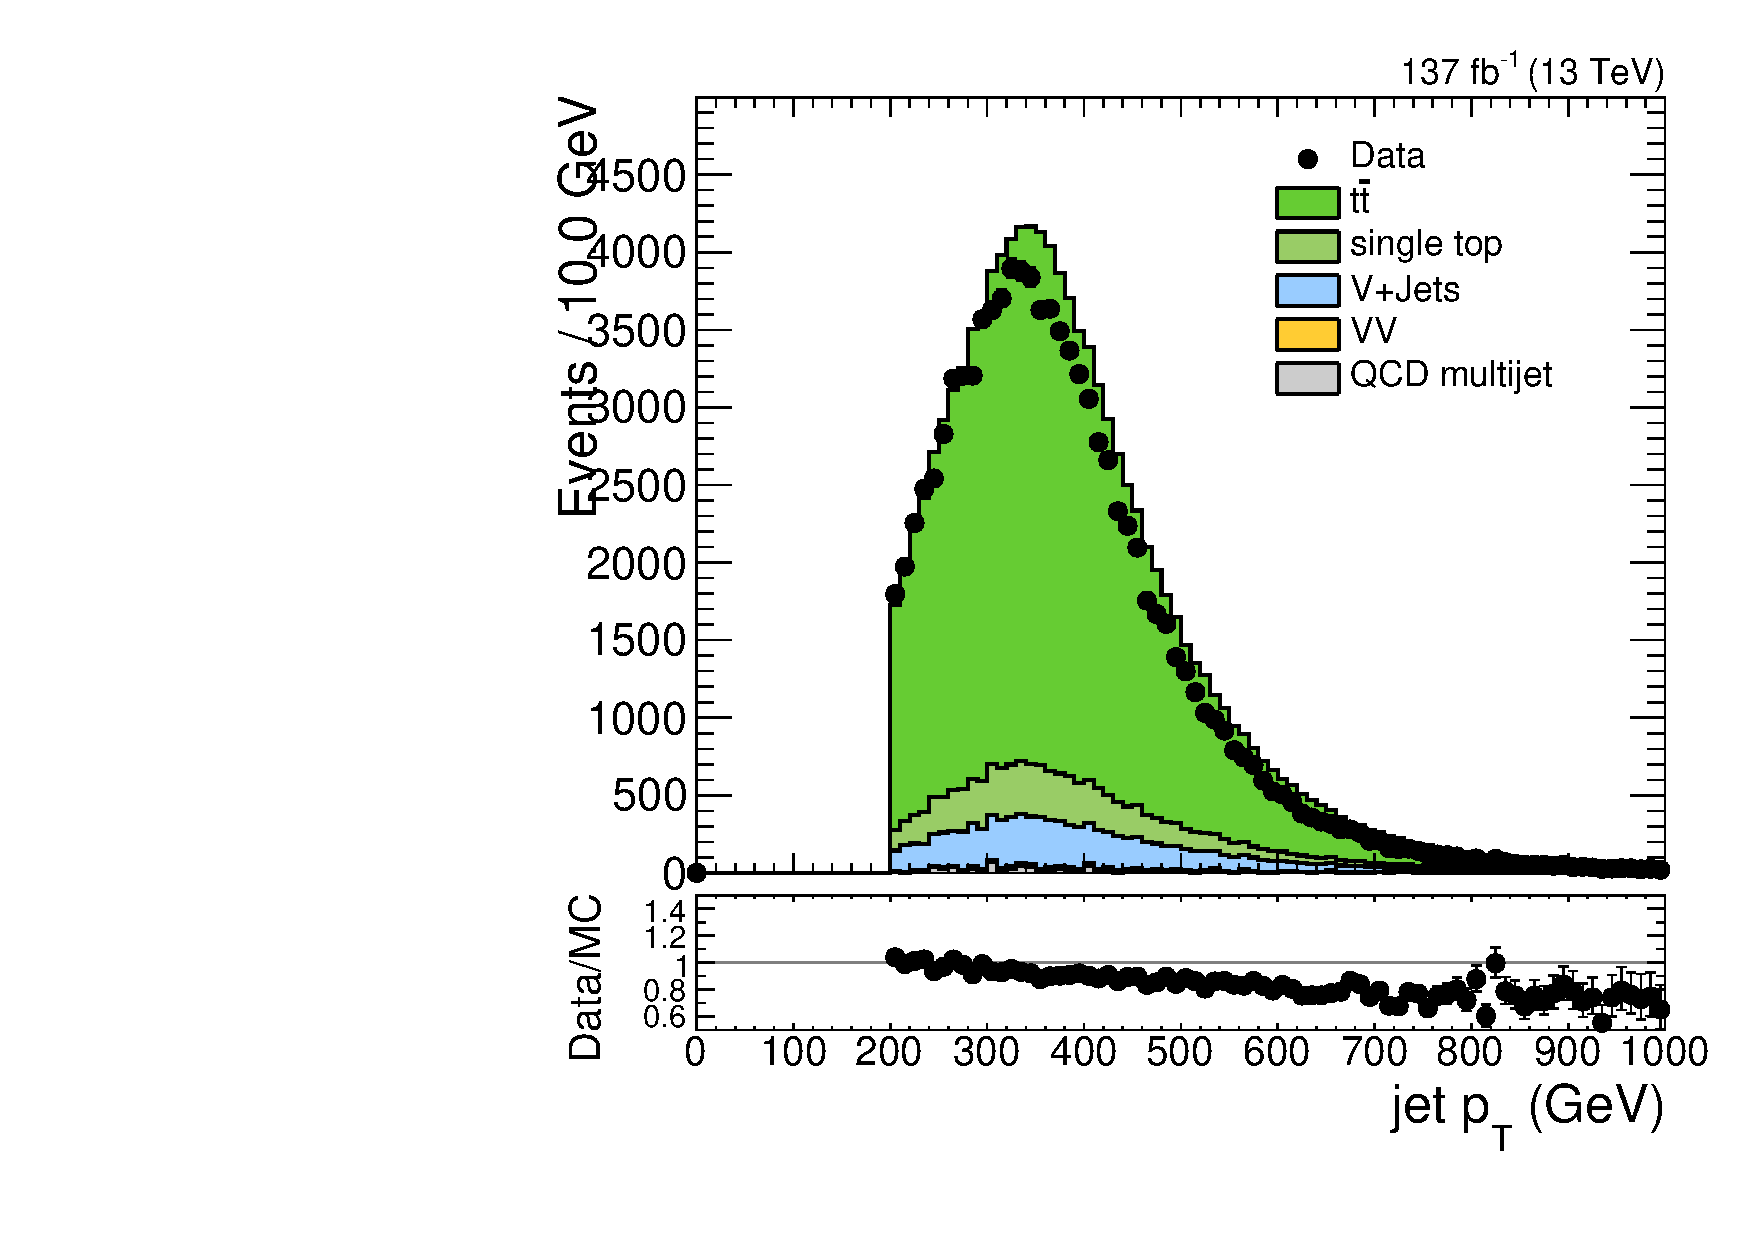
\includegraphics[width=0.3825\textwidth]{fig/analysisAppendix/CR_b1_allL_allP_allC_allD_Run2_lnujj_l2_pt.pdf}
  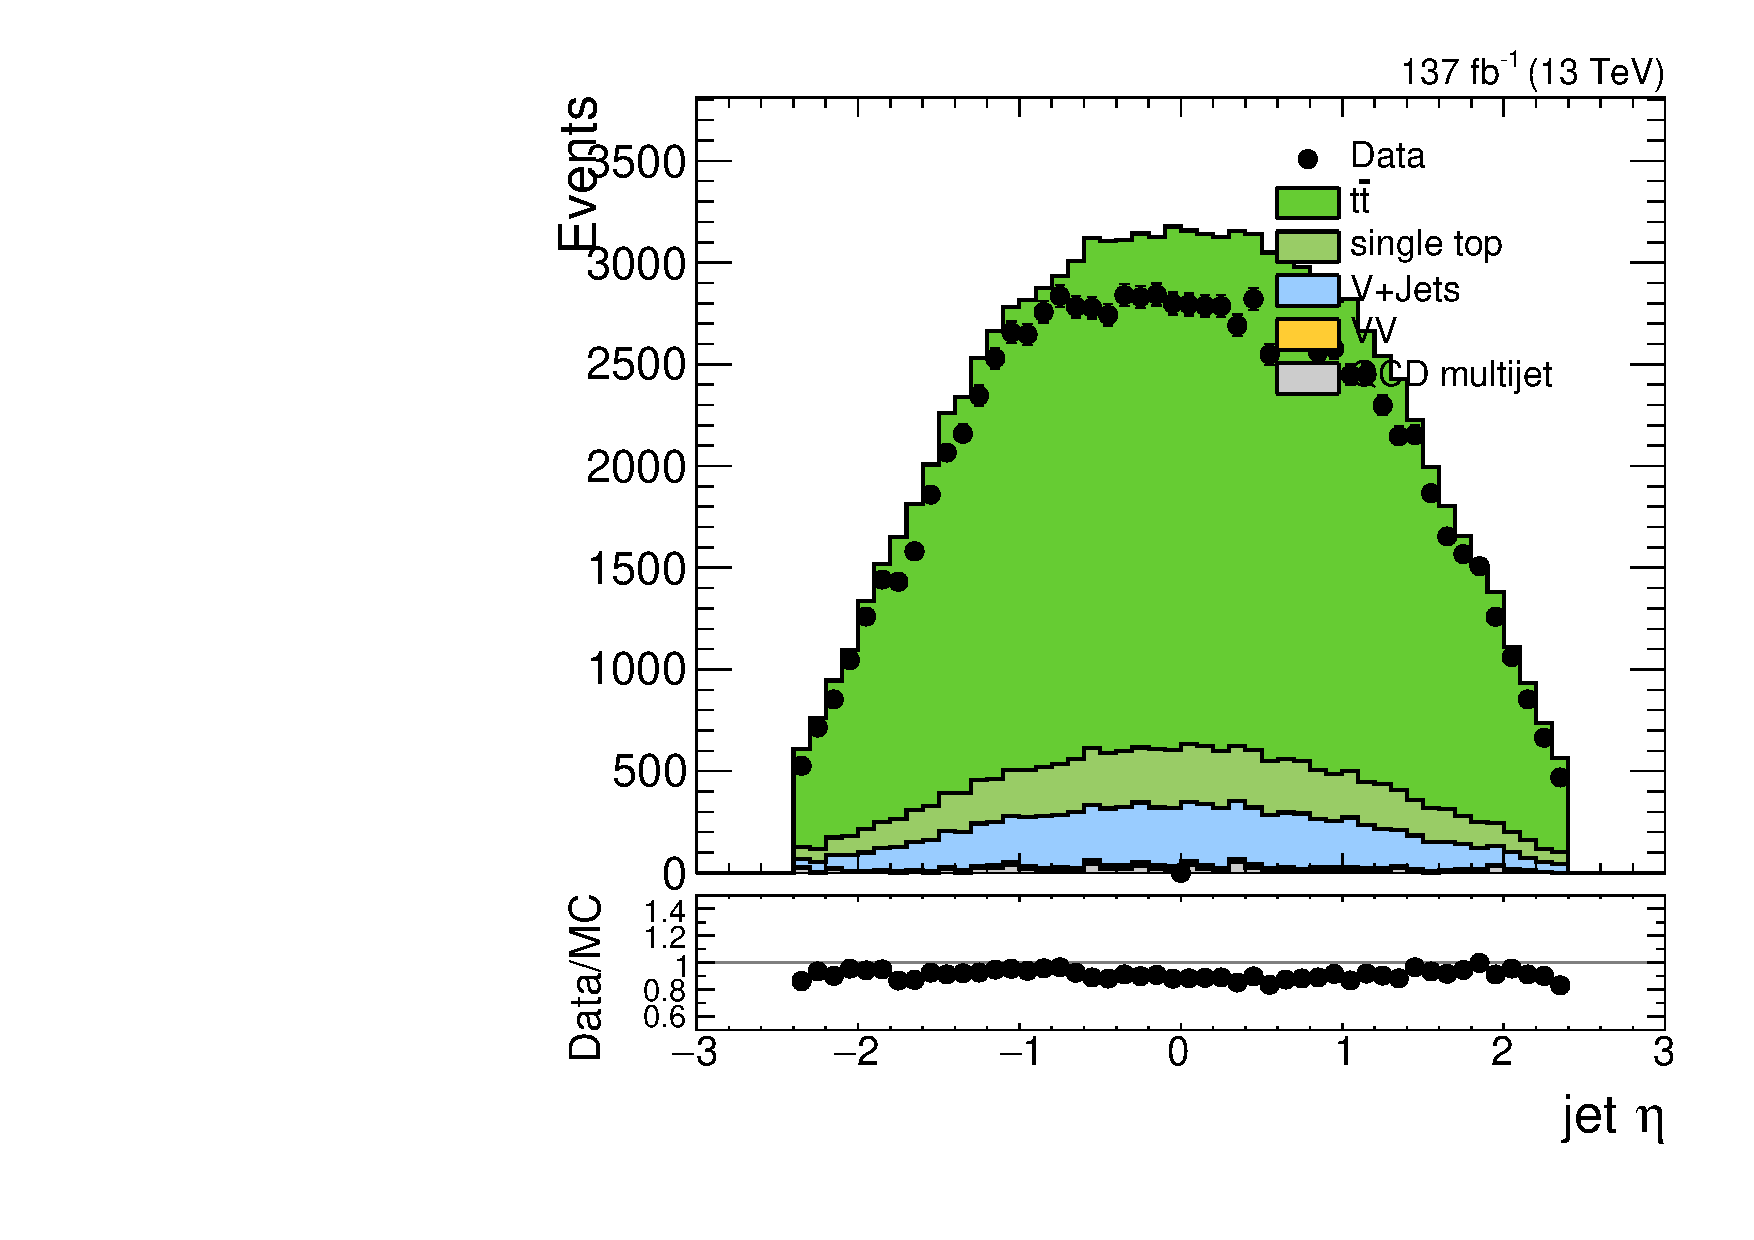
\includegraphics[width=0.3825\textwidth]{fig/analysisAppendix/CR_b1_allL_allP_allC_allD_Run2_lnujj_l2_eta.pdf}\\
  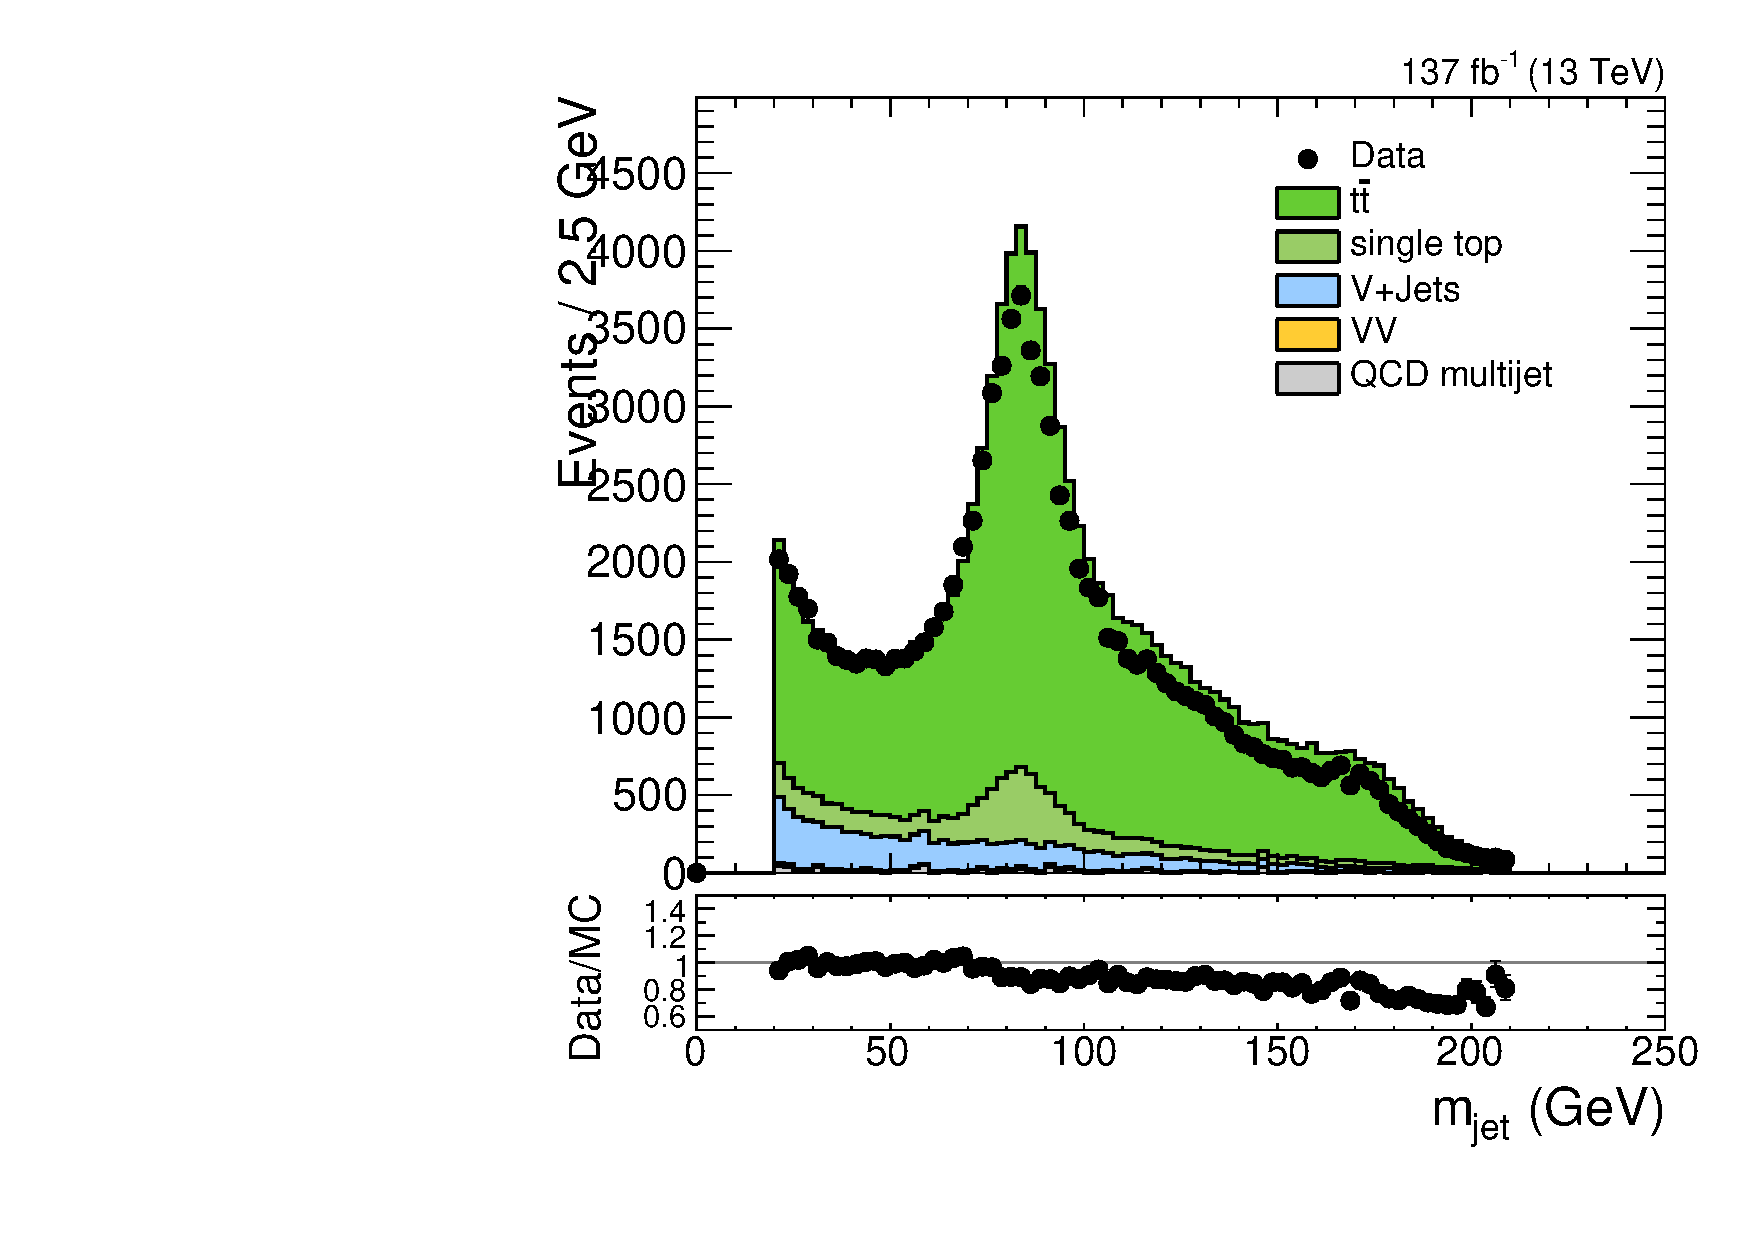
\includegraphics[width=0.3825\textwidth]{fig/analysisAppendix/CR_b1_allL_allP_allC_allD_Run2_mjet.pdf}\\
  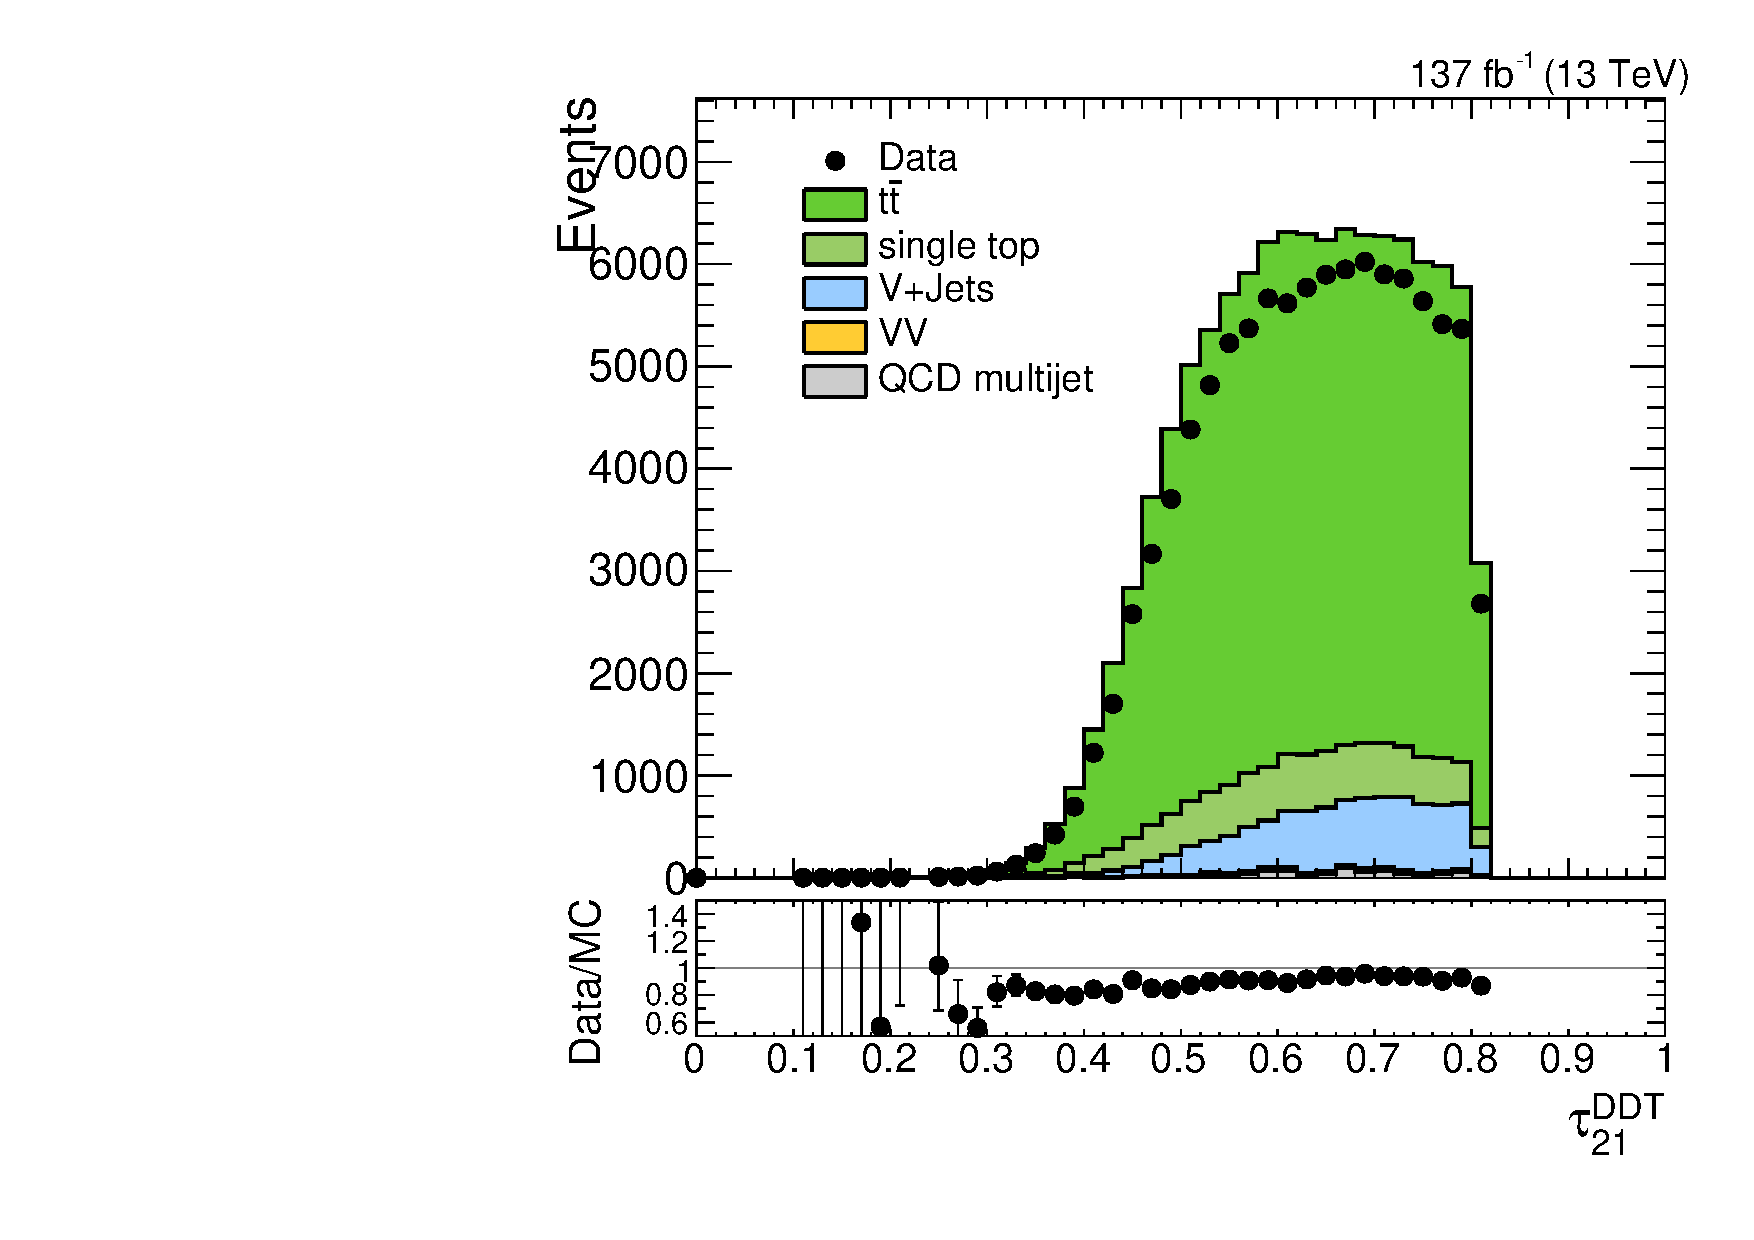
\includegraphics[width=0.3825\textwidth]{fig/analysisAppendix/CR_b1_allL_allP_allC_allD_Run2_tau21DDT.pdf}
  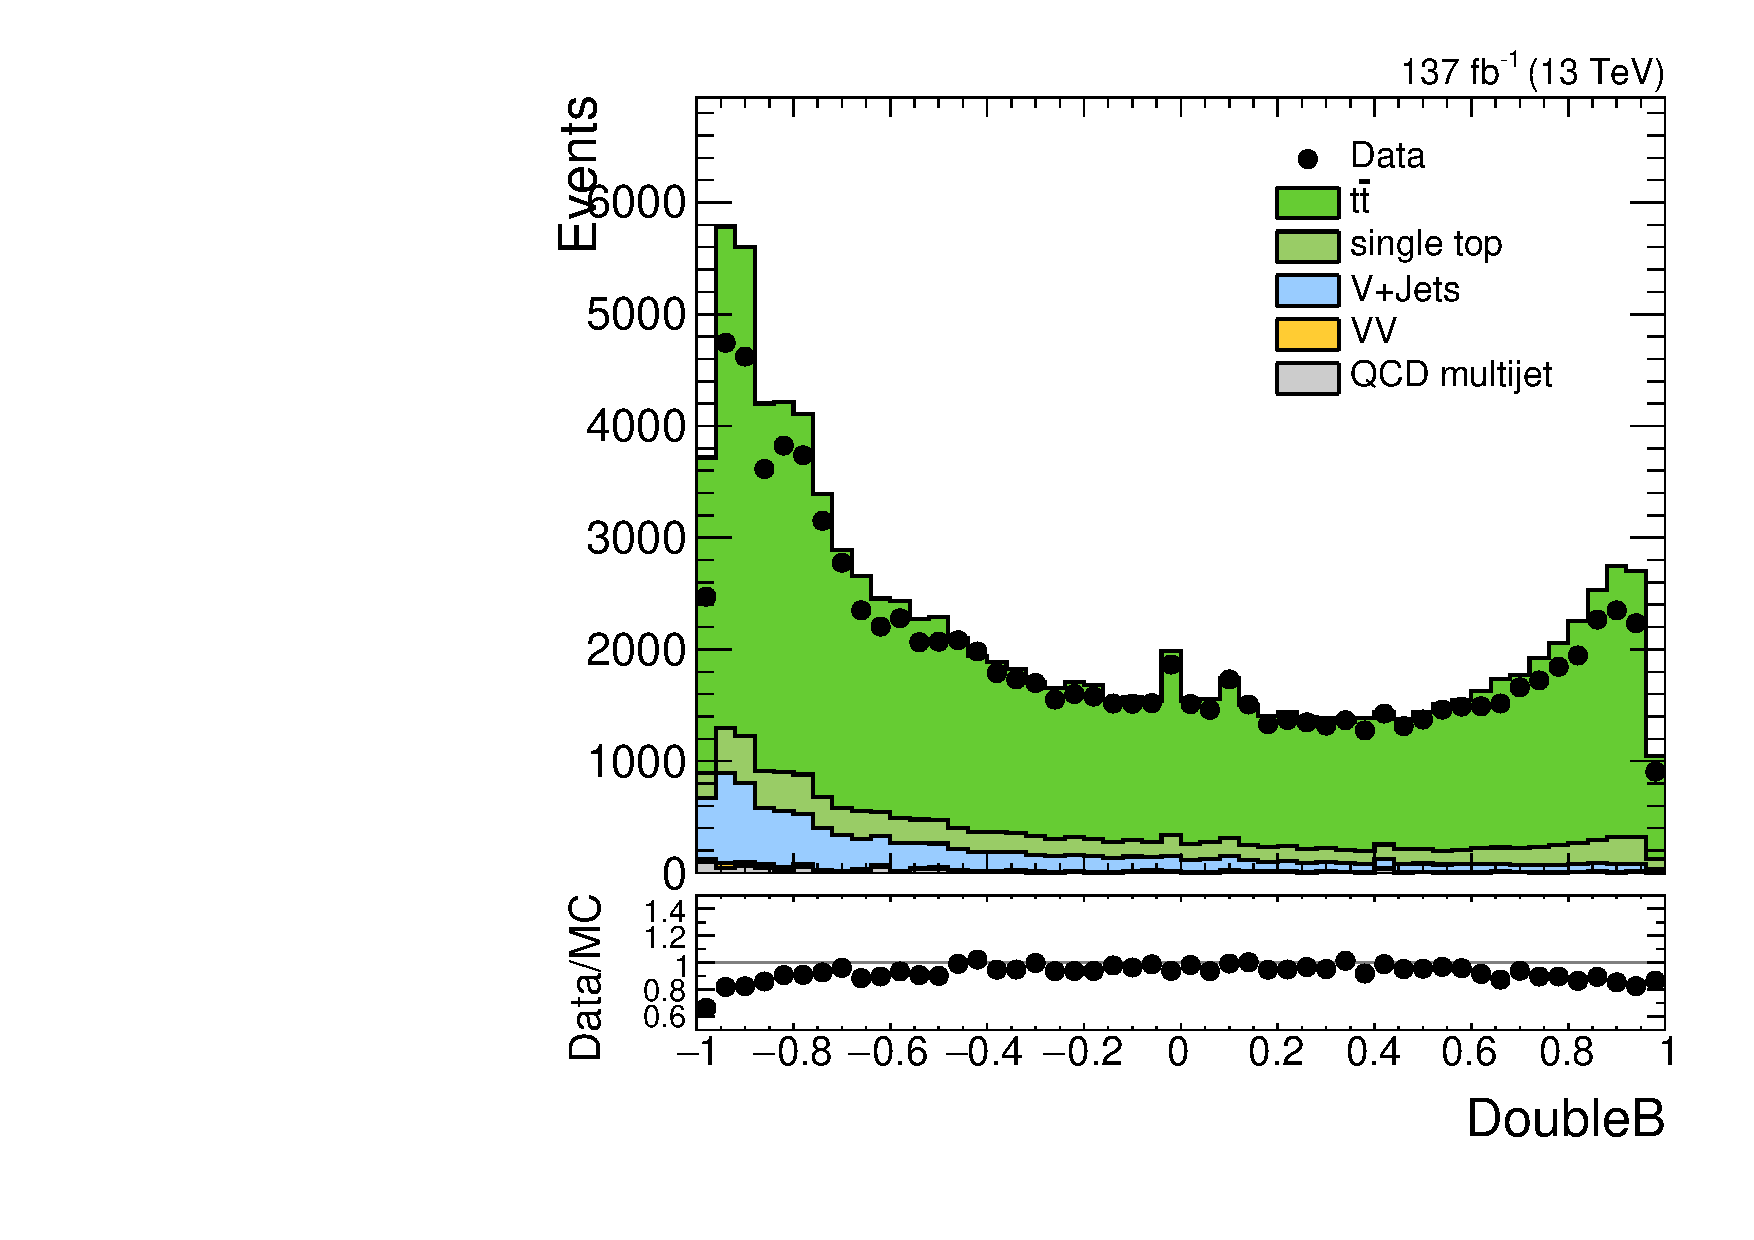
\includegraphics[width=0.3825\textwidth]{fig/analysisAppendix/CR_b1_allL_allP_allC_allD_Run2_DoubleB.pdf}\\
  \caption{
    Comparison plots between data and MC from Run 2 for the \pt, $\eta$, \MJ (soft drop mass), \nsubjDDT, and \DoubleB tagger of the selected \Vhad candidate (leading AK8 jet), in the top-enriched control region.
  }
  \label{fig:CR_controlPlotsRun2_3}
\end{figure}

\begin{figure}[htbp]
  \centering
  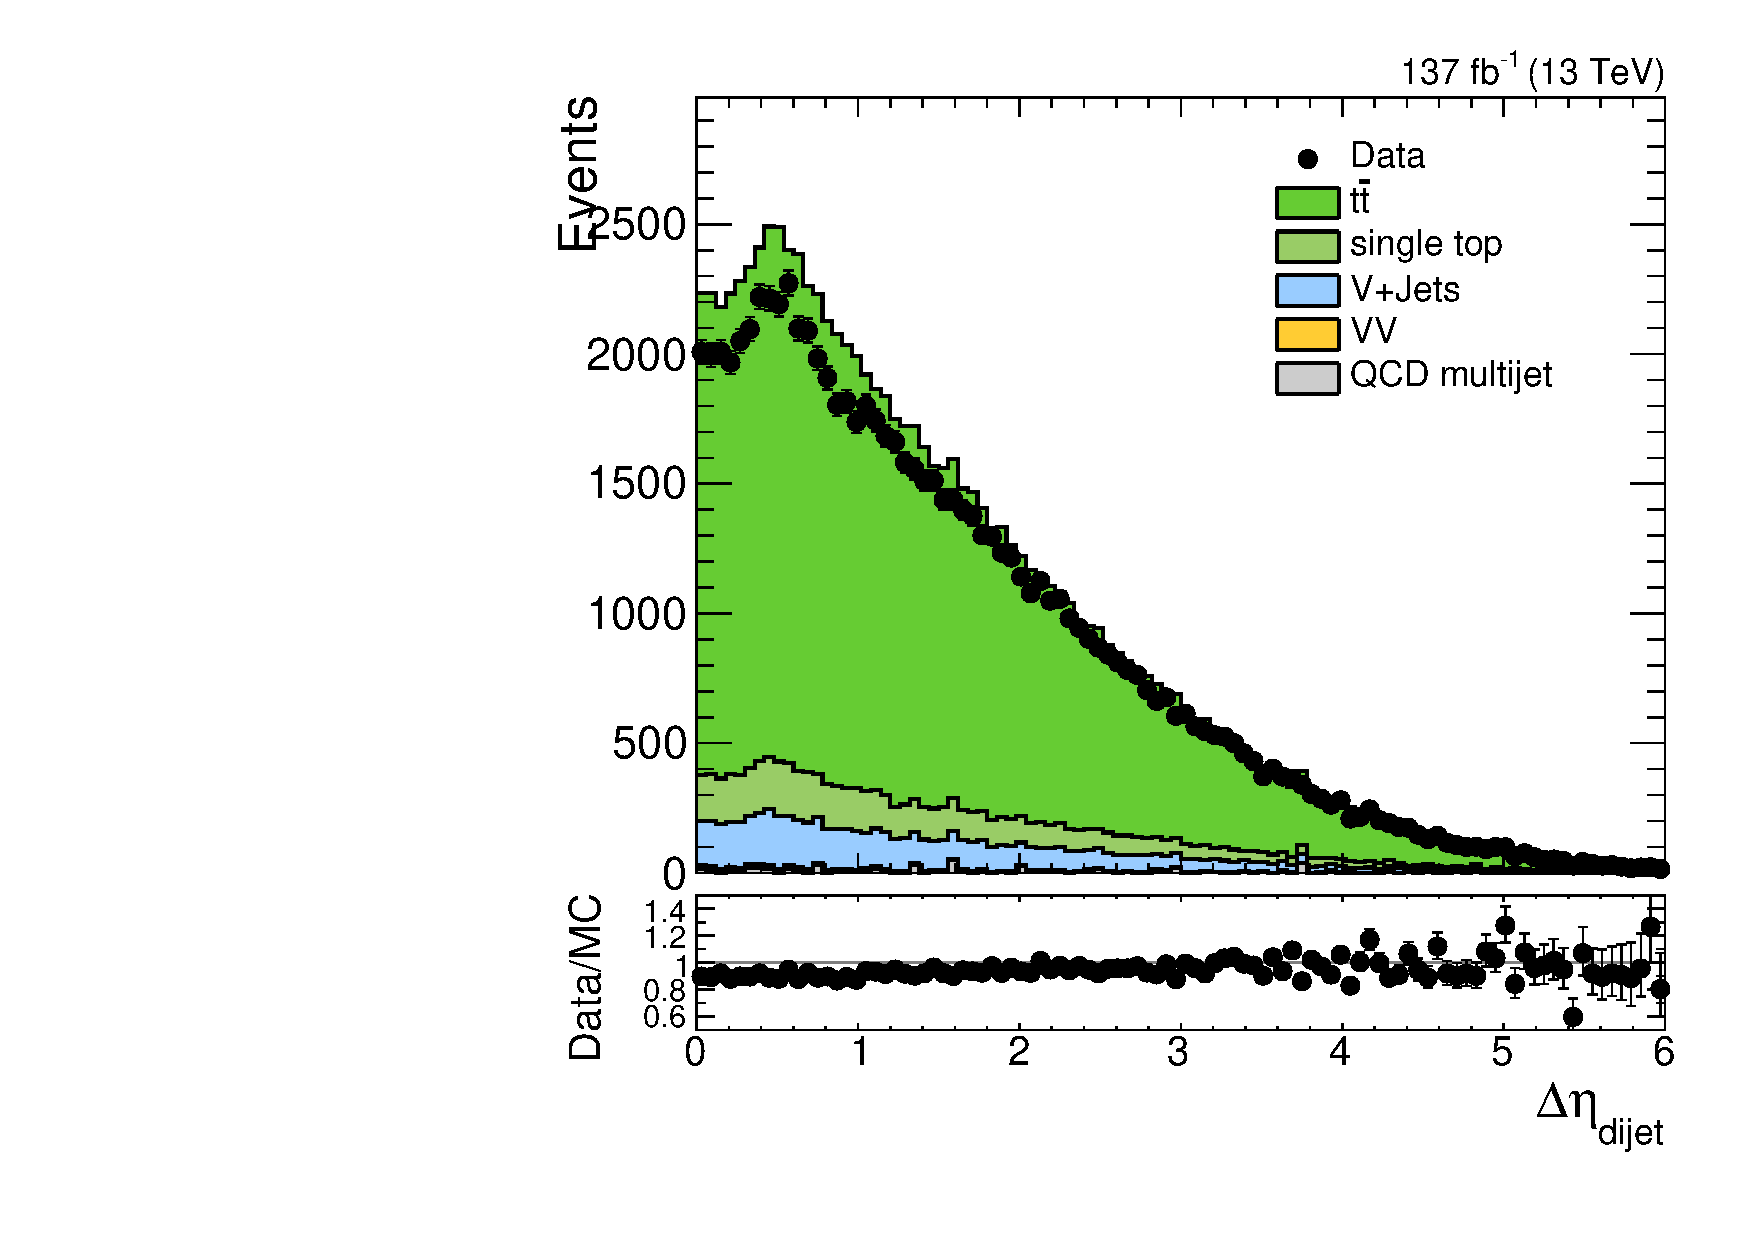
\includegraphics[width=0.3825\textwidth]{fig/analysisAppendix/CR_b1_allL_allP_allC_allD_Run2_lnujj_vbfDEta.pdf}
  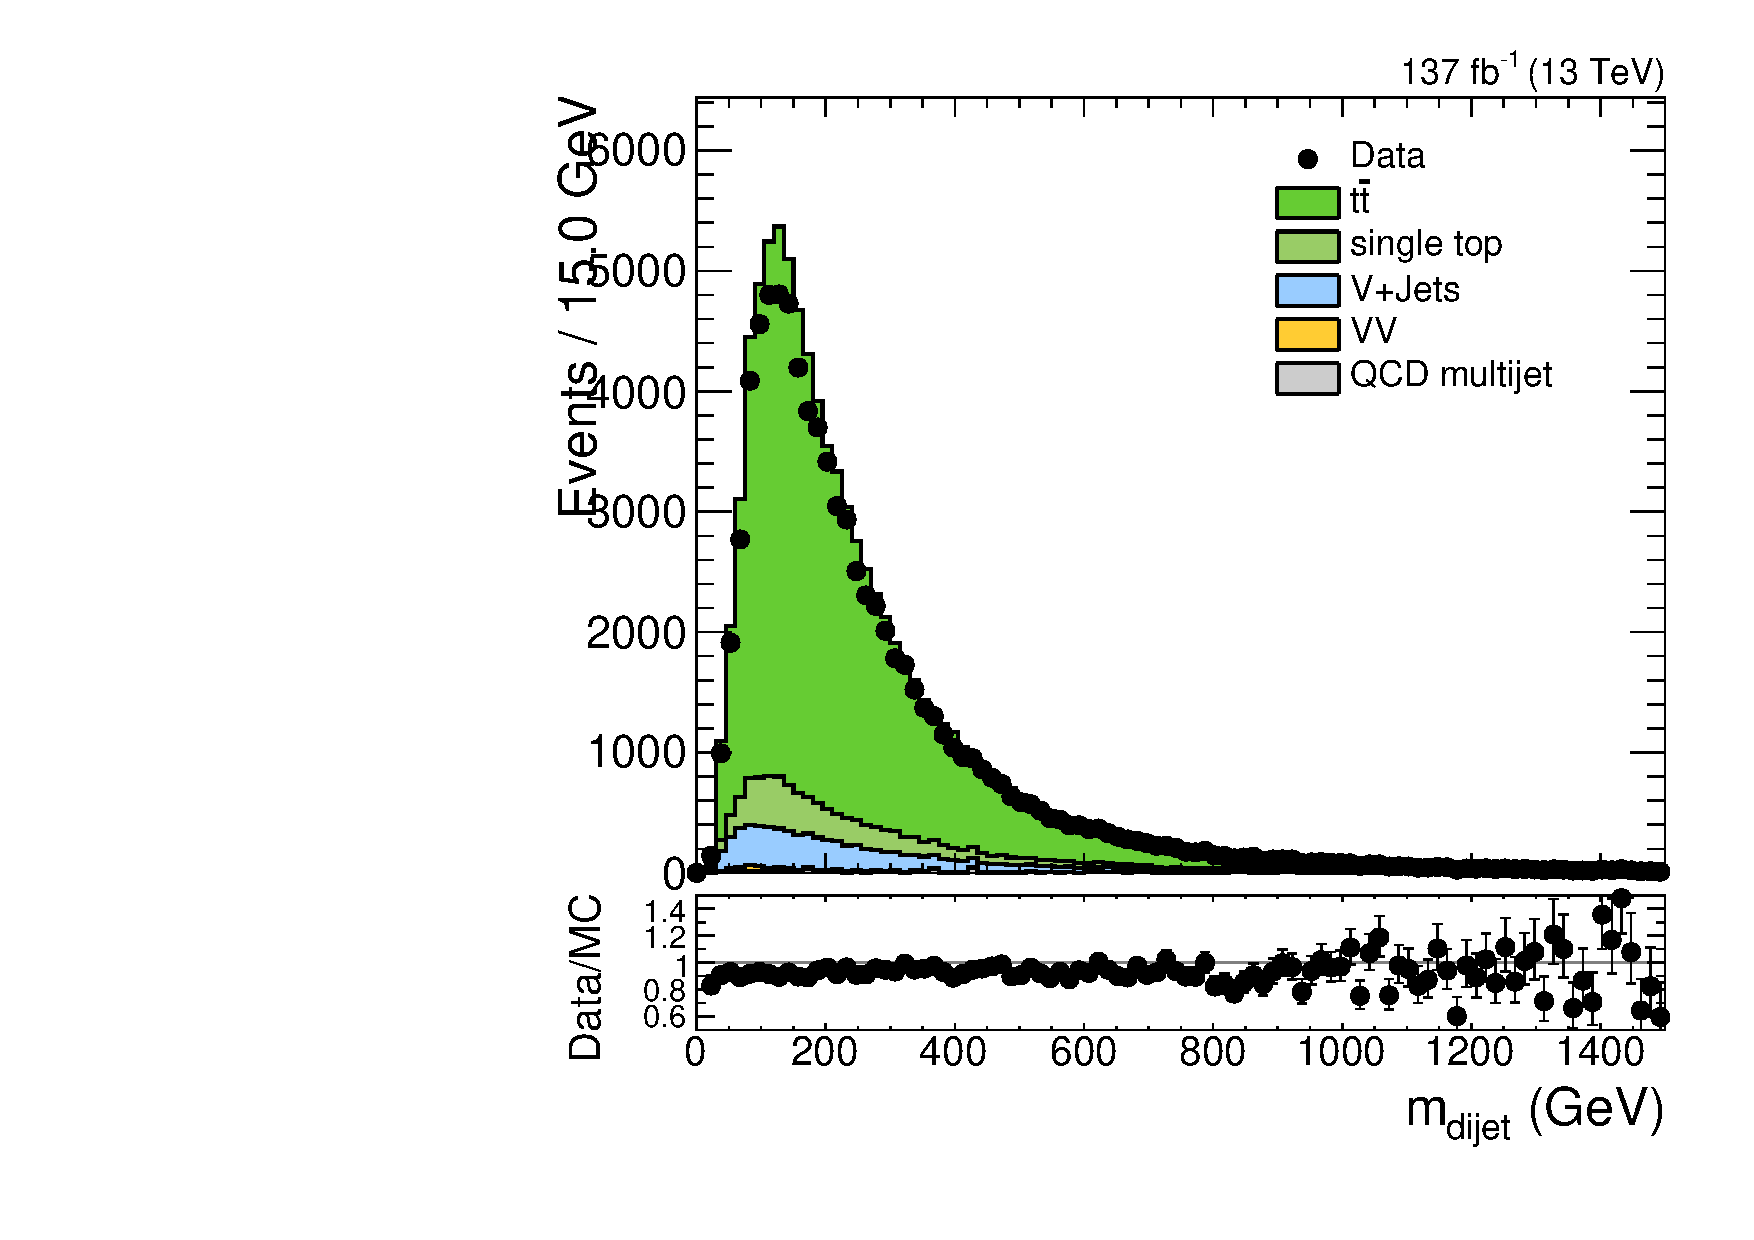
\includegraphics[width=0.3825\textwidth]{fig/analysisAppendix/CR_b1_allL_allP_allC_allD_Run2_lnujj_vbfMass.pdf}\\
  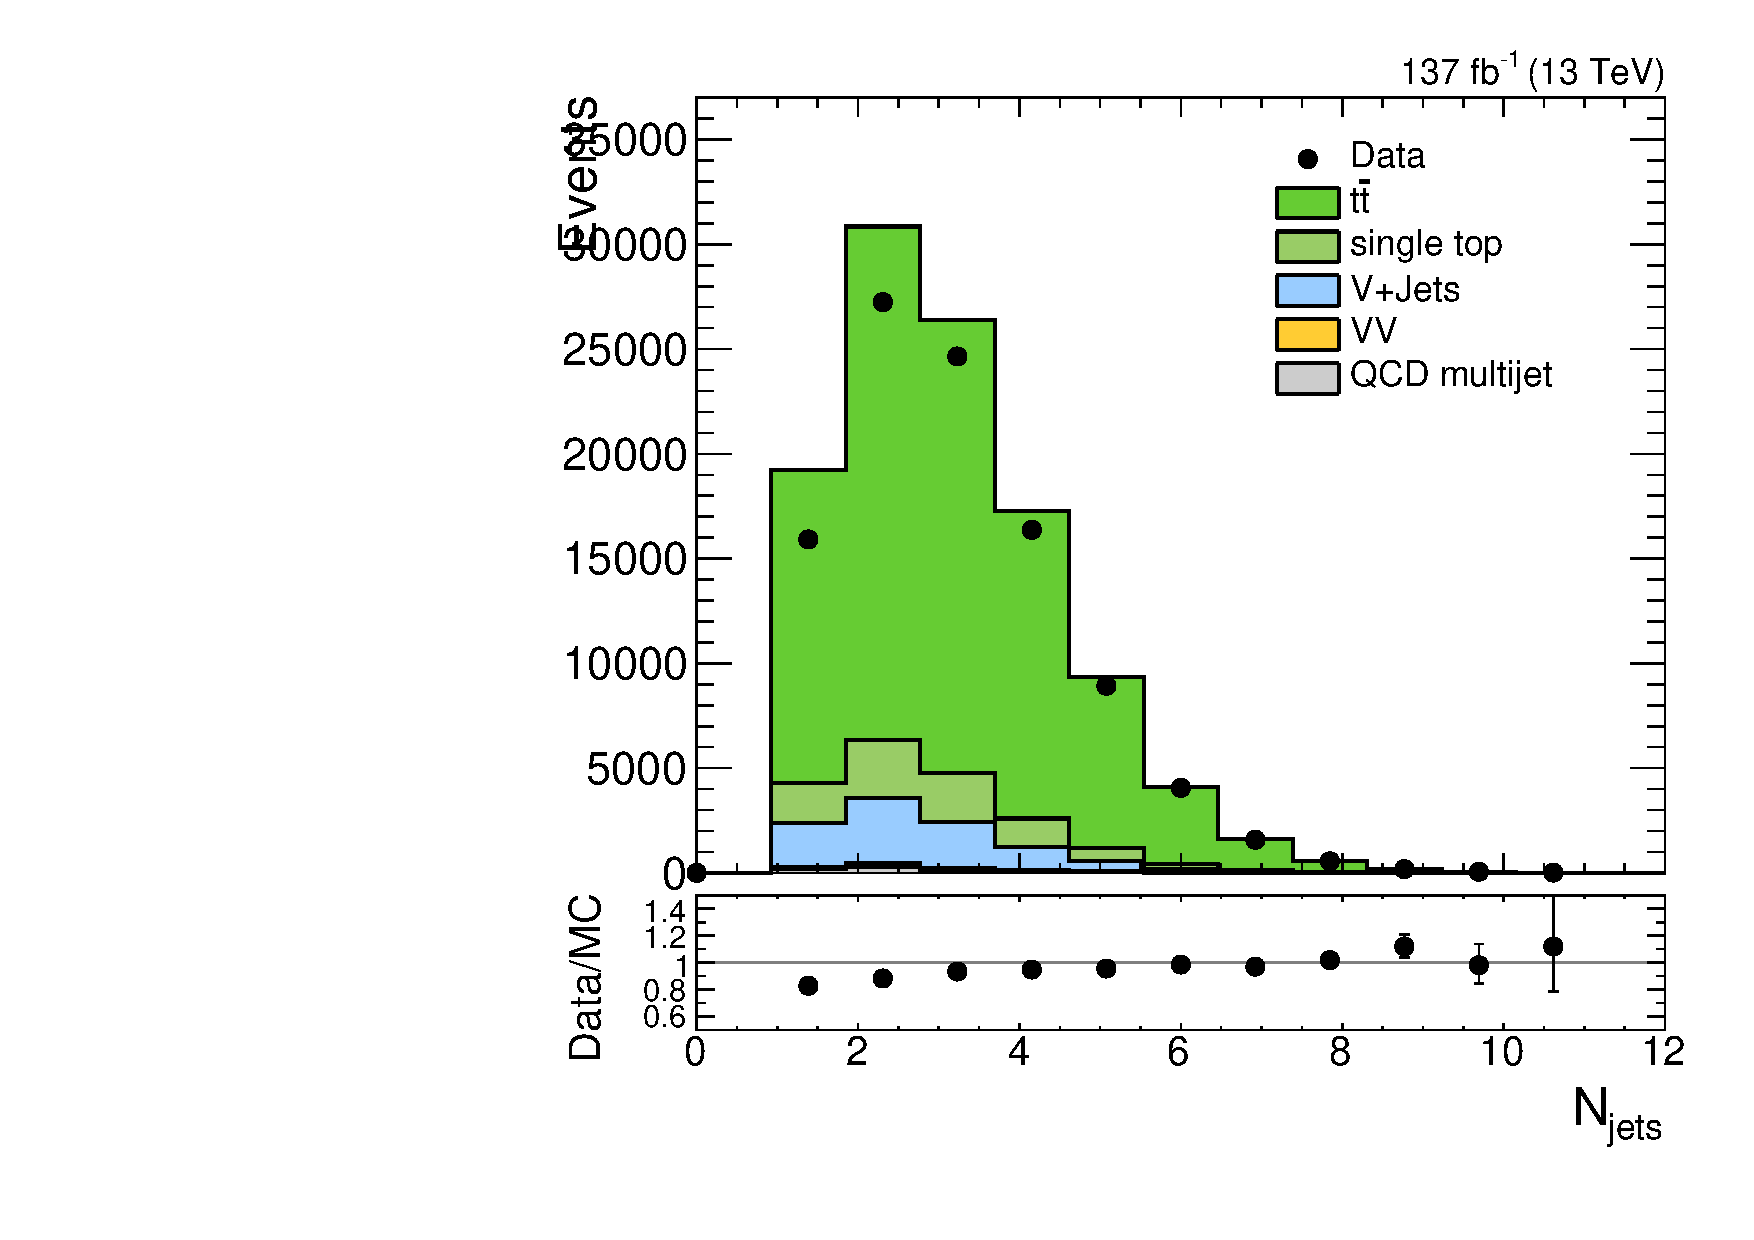
\includegraphics[width=0.3825\textwidth]{fig/analysisAppendix/CR_b1_allL_allP_allC_allD_Run2_lnujj_nJets.pdf}
  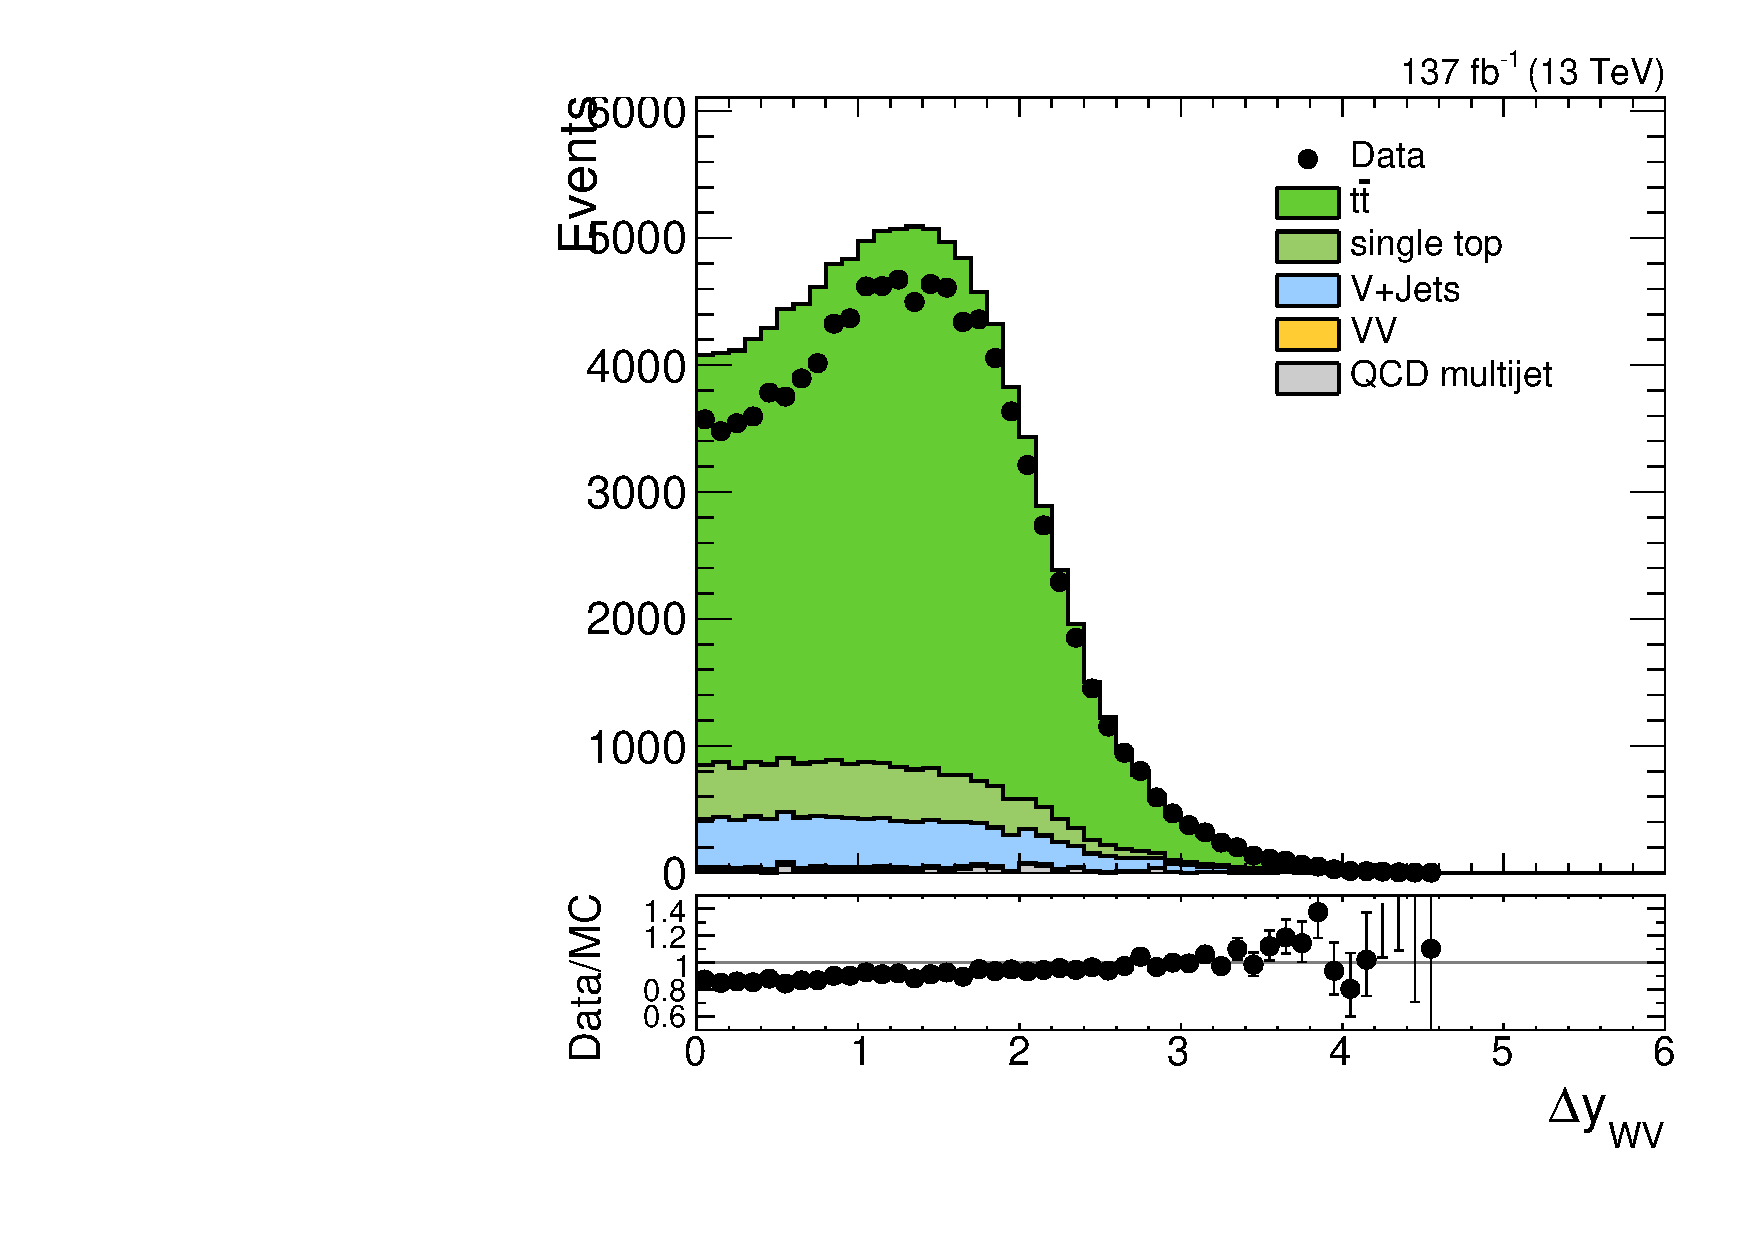
\includegraphics[width=0.3825\textwidth]{fig/analysisAppendix/CR_b1_allL_allP_allC_allD_Run2_dy.pdf}\\
  \caption{
    Comparison plots between data and MC from Run 2 for the separation in $\eta$ of the \VBF forward jets, invariant mass of the \VBF jets, number of selected standard jets, and rapidity separation between the reconstructed bosons, in the top-enriched control region.
  }
  \label{fig:CR_controlPlotsRun2_4}
\end{figure}

\section{Two-dimensional Fit Process}

\subsection{Signal Shapes}

% Analytic signal shape figures
Figures \ref{fig:MVVShapes_NonVBF_LDy} and \ref{fig:MVVShapes_NonVBF_HDy} show the \MVV signal shapes for non-\VBF signals.
For figures \ref{fig:MVVShapes_VBF_LDy} and \ref{fig:MVVShapes_VBF_HDy}, we show the \MVV signal shapes for the \VBF signals.
In figures \ref{fig:MJJShapes_NonVBF_LDy} and \ref{fig:MJJShapes_NonVBF_HDy}, the \MJ signal shapes are shown for the non-\VBF signals.
Finally, figures \ref{fig:MJJShapes_VBF_LDy} and \ref{fig:MJJShapes_VBF_HDy} show the \MJ signal shapes for the \VBF signals.
We also perform a closure test by converting the \MVV and \MJ projections of the $2\unit{TeV}$ version of the template of each signal model into 1D histograms and compare them with the corresponding weighted MC distributions for each category in figures~\ref{fig:1dtemplateVsReco_GbuToWW2000}-\ref{fig:1dtemplateVsReco_VBFWprToWZ2000}.

\begin{figure}[htbp]
  \centering
  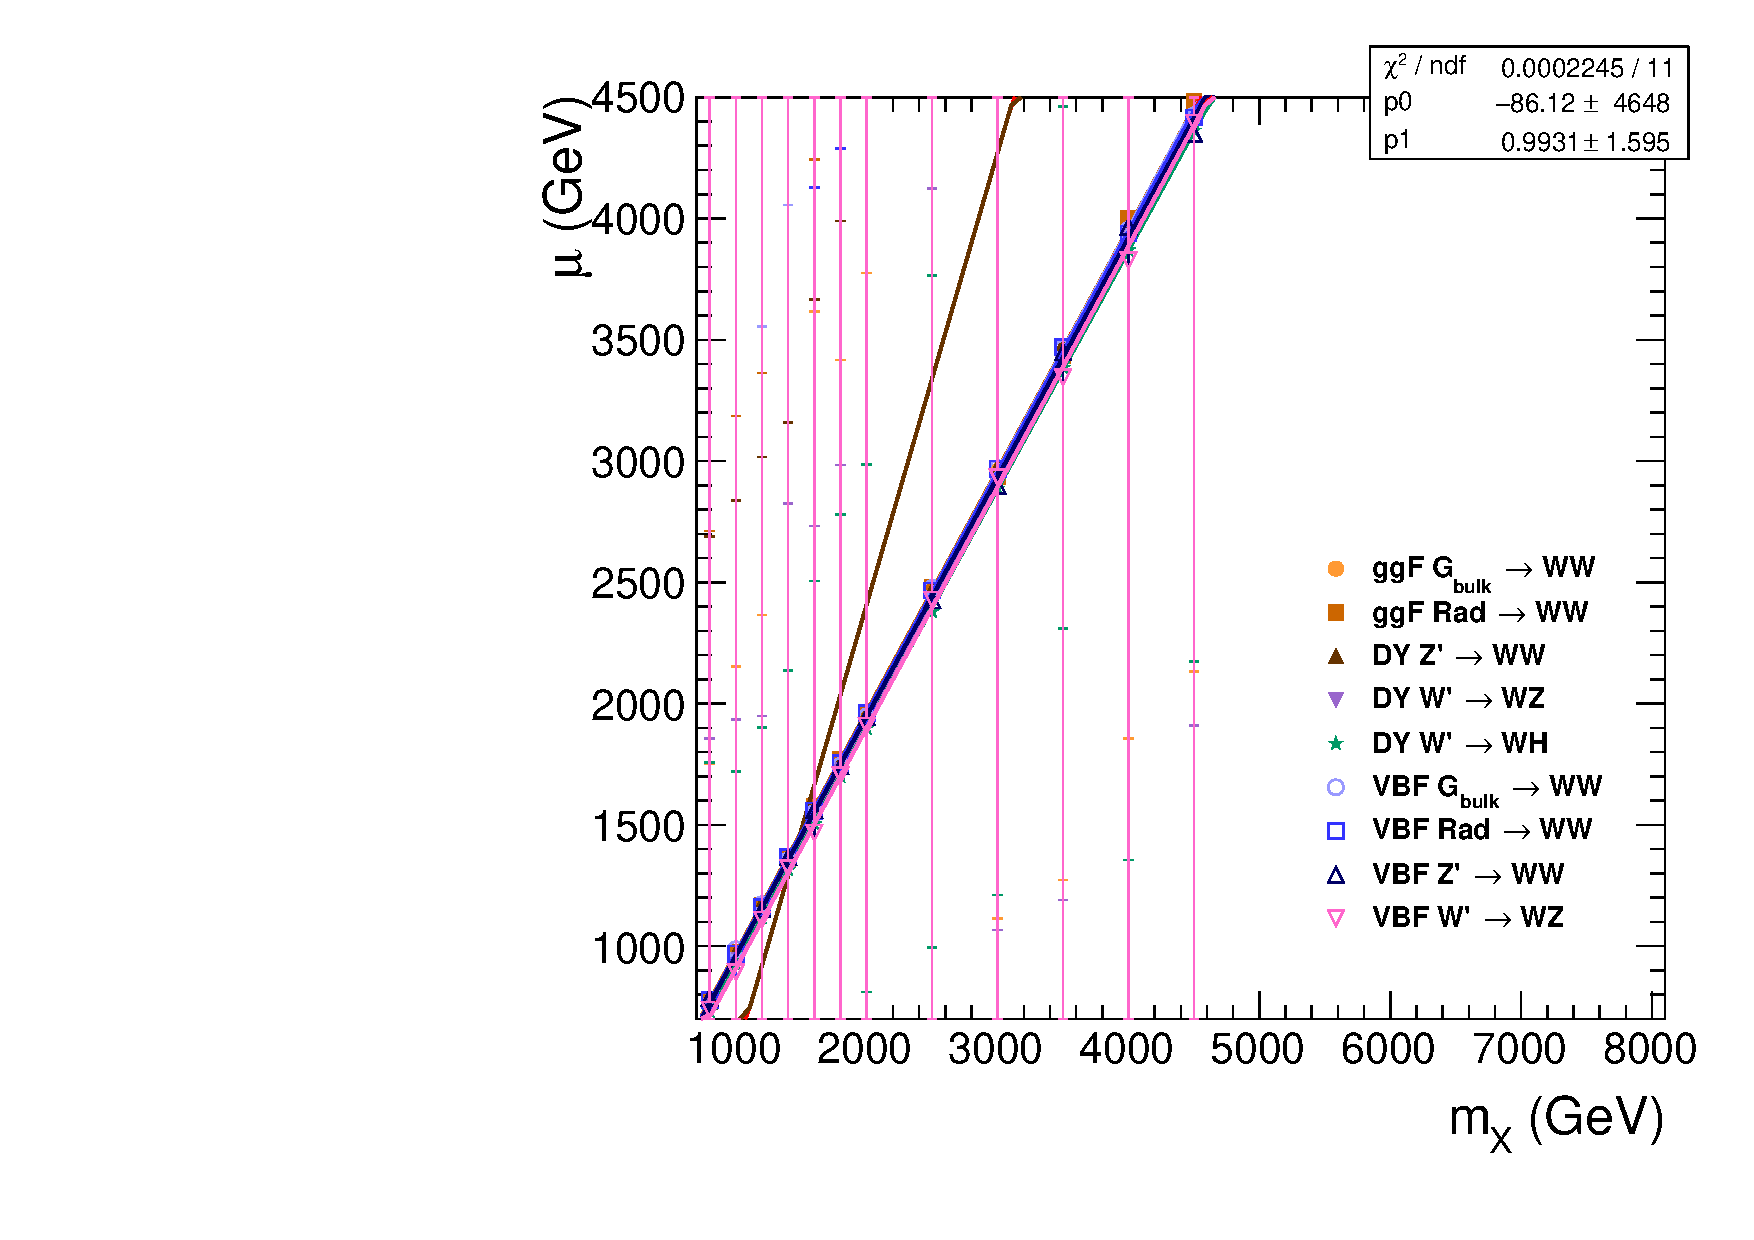
\includegraphics[width=0.2\textwidth]{fig/analysisAppendix/paramSignalShape_allSig_MVV_HP_bb_LDy_MEAN.pdf}
  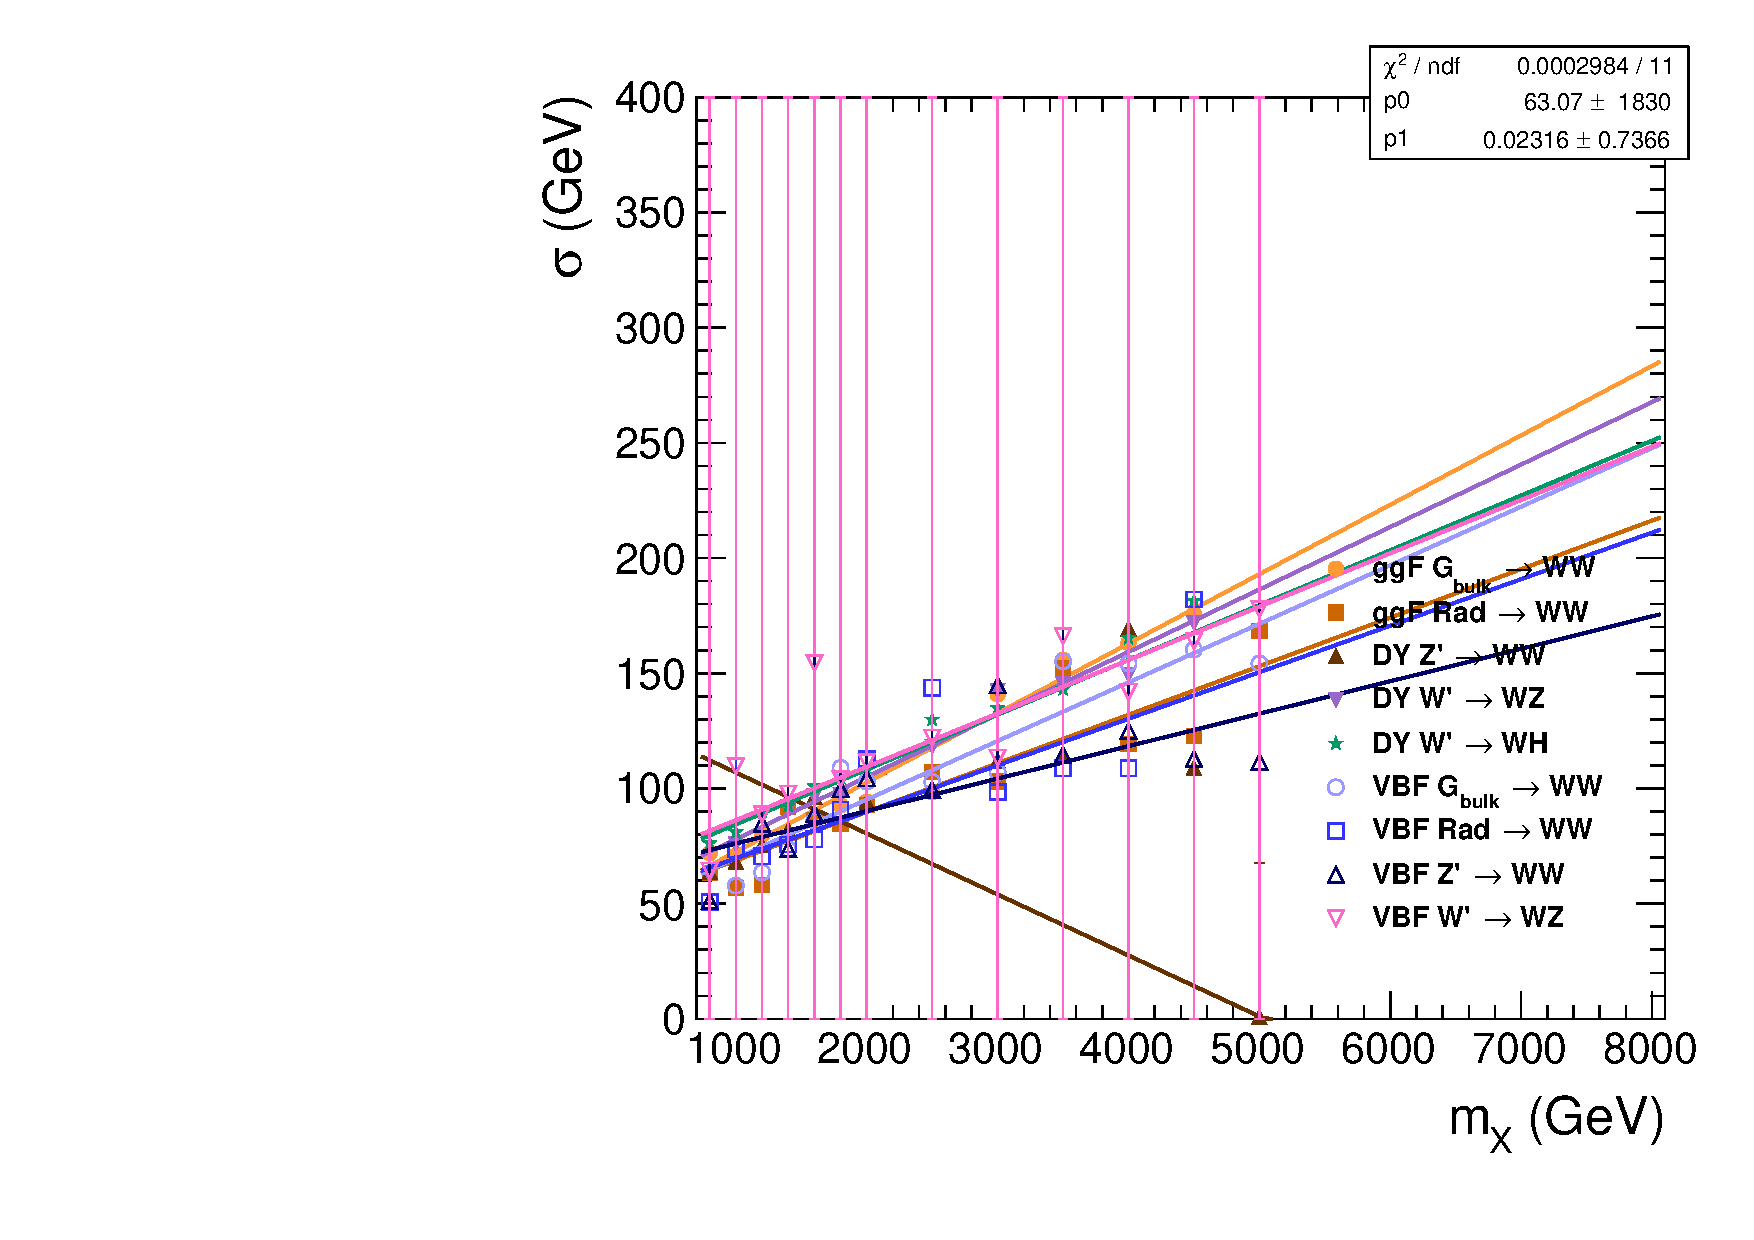
\includegraphics[width=0.2\textwidth]{fig/analysisAppendix/paramSignalShape_allSig_MVV_HP_bb_LDy_SIGMA.pdf}
  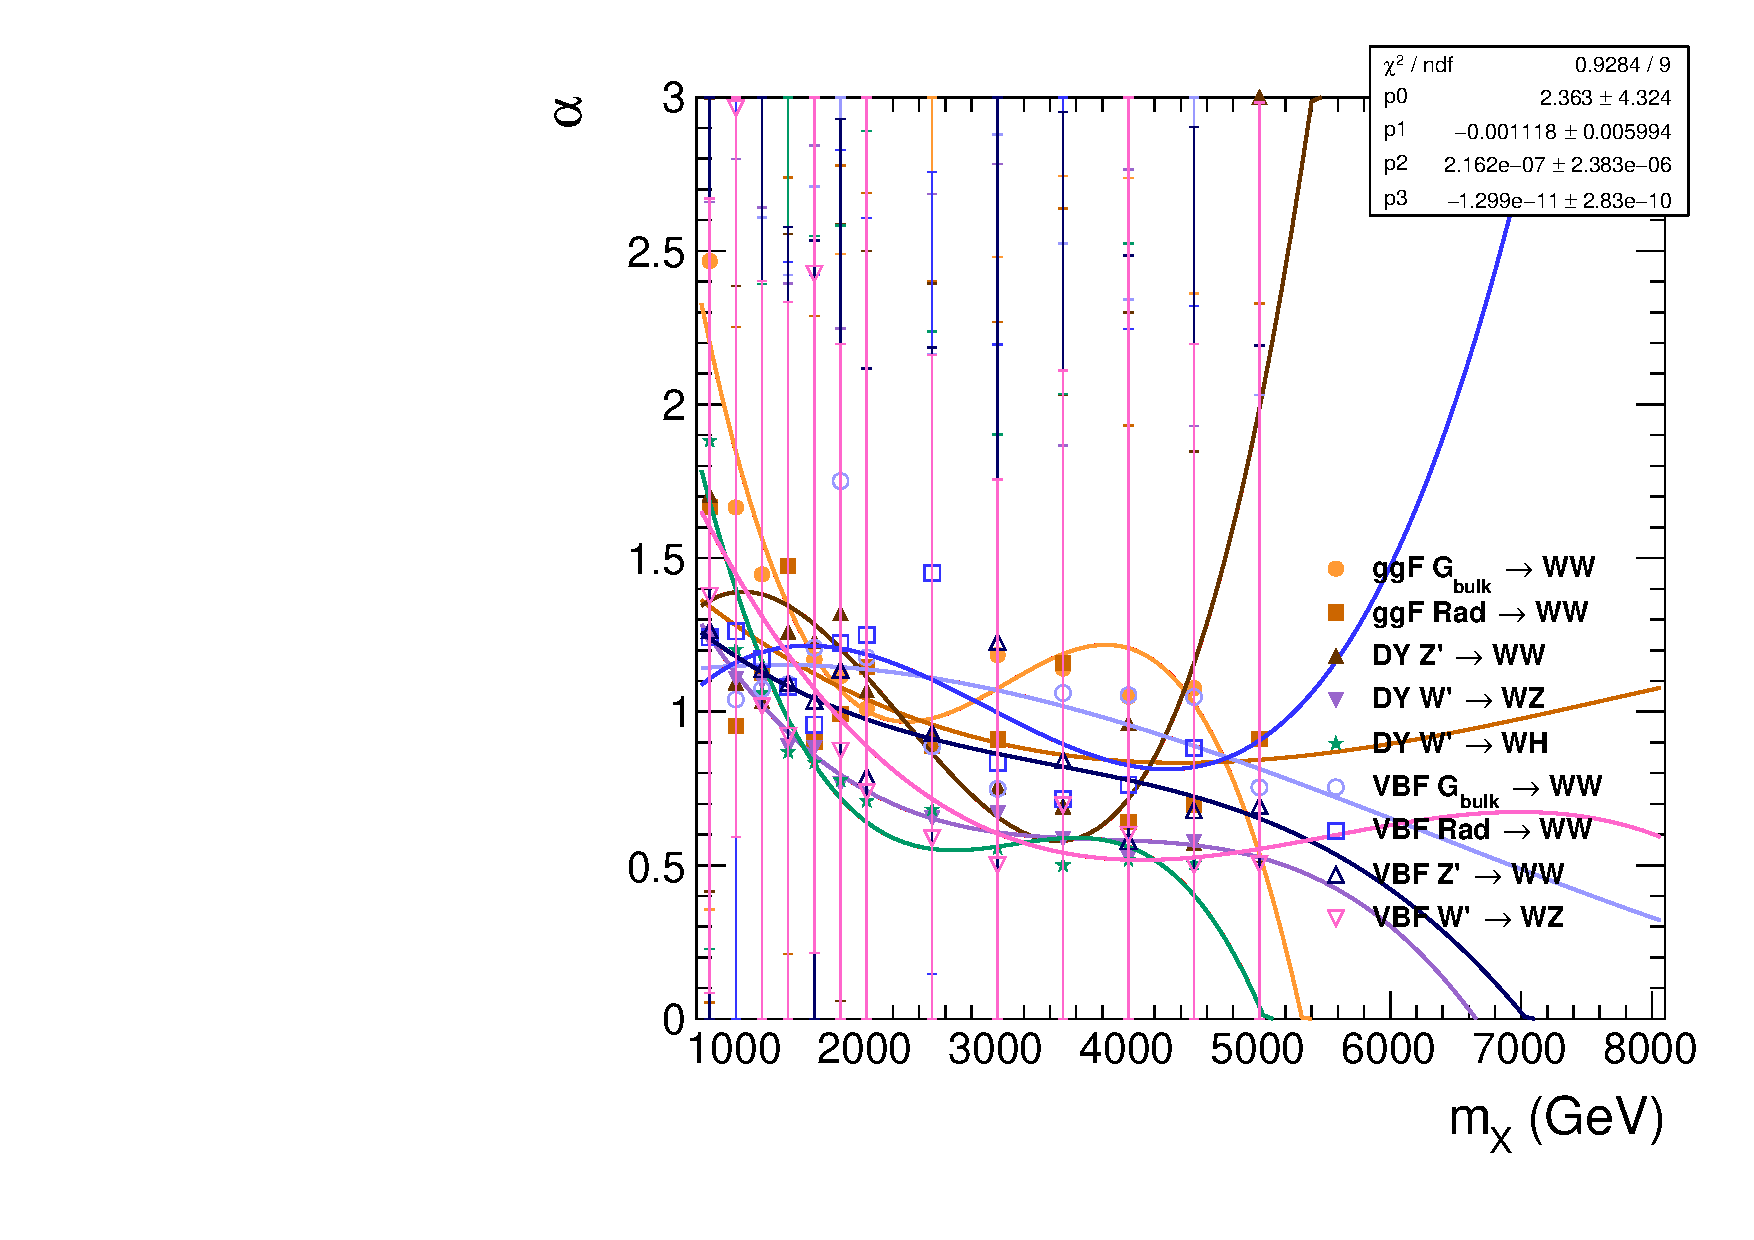
\includegraphics[width=0.2\textwidth]{fig/analysisAppendix/paramSignalShape_allSig_MVV_HP_bb_LDy_ALPHA1.pdf}
  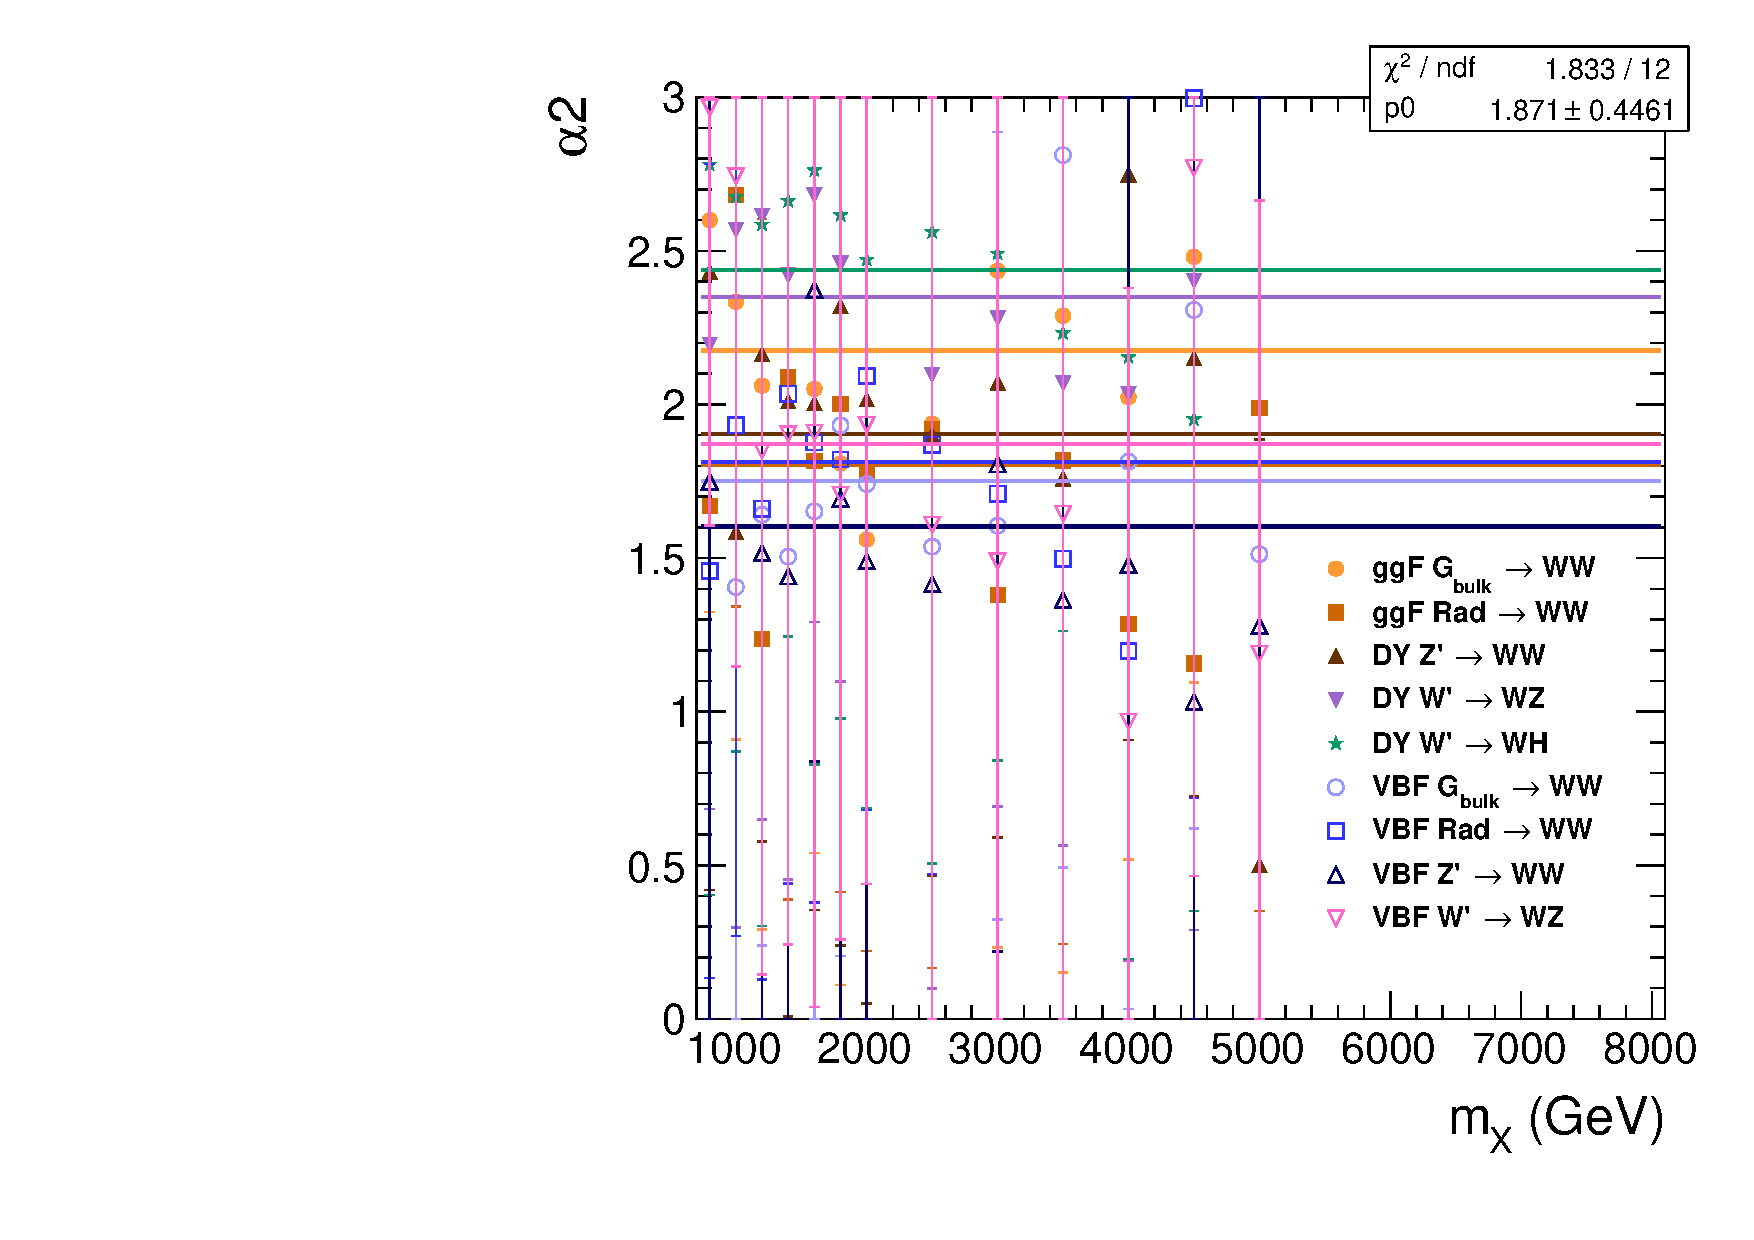
\includegraphics[width=0.2\textwidth]{fig/analysisAppendix/paramSignalShape_allSig_MVV_HP_bb_LDy_ALPHA2.pdf}\\
  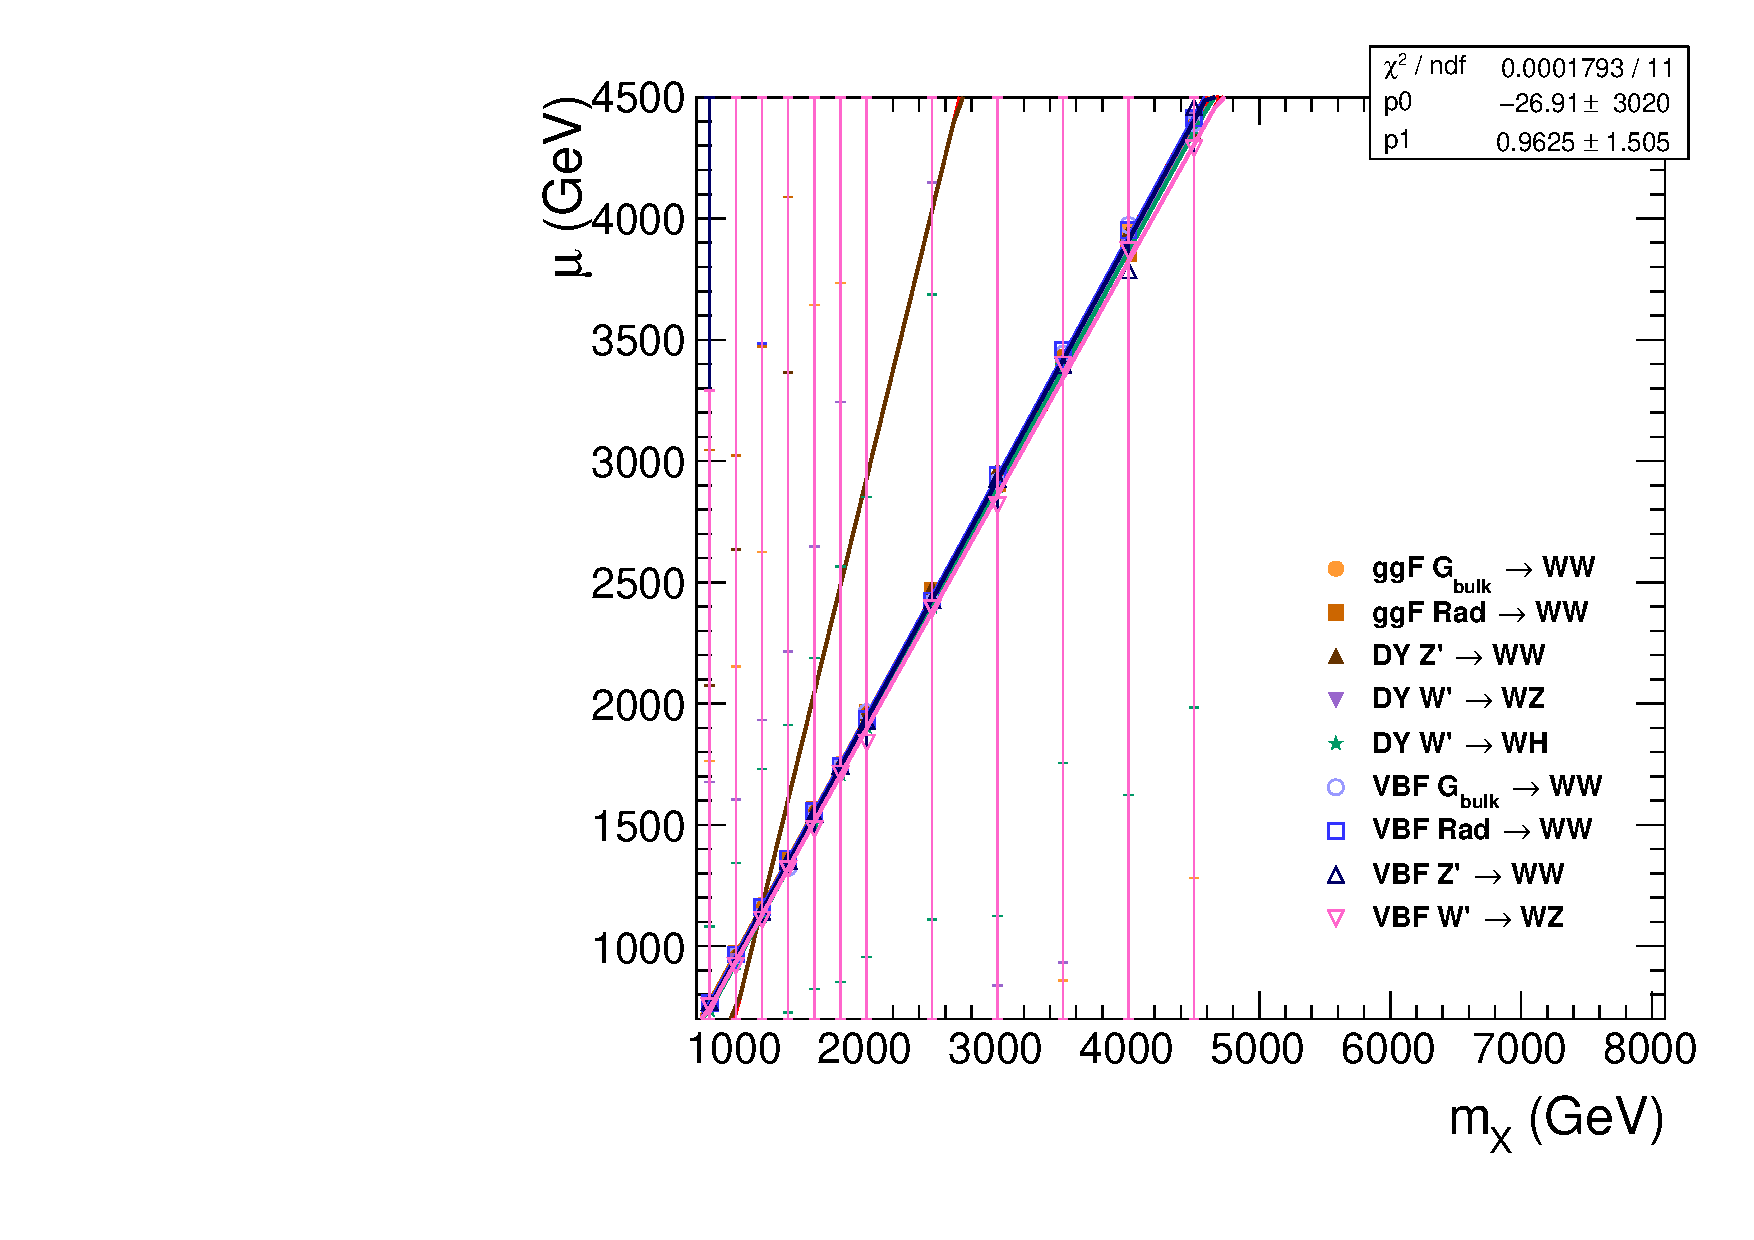
\includegraphics[width=0.2\textwidth]{fig/analysisAppendix/paramSignalShape_allSig_MVV_LP_bb_LDy_MEAN.pdf}
  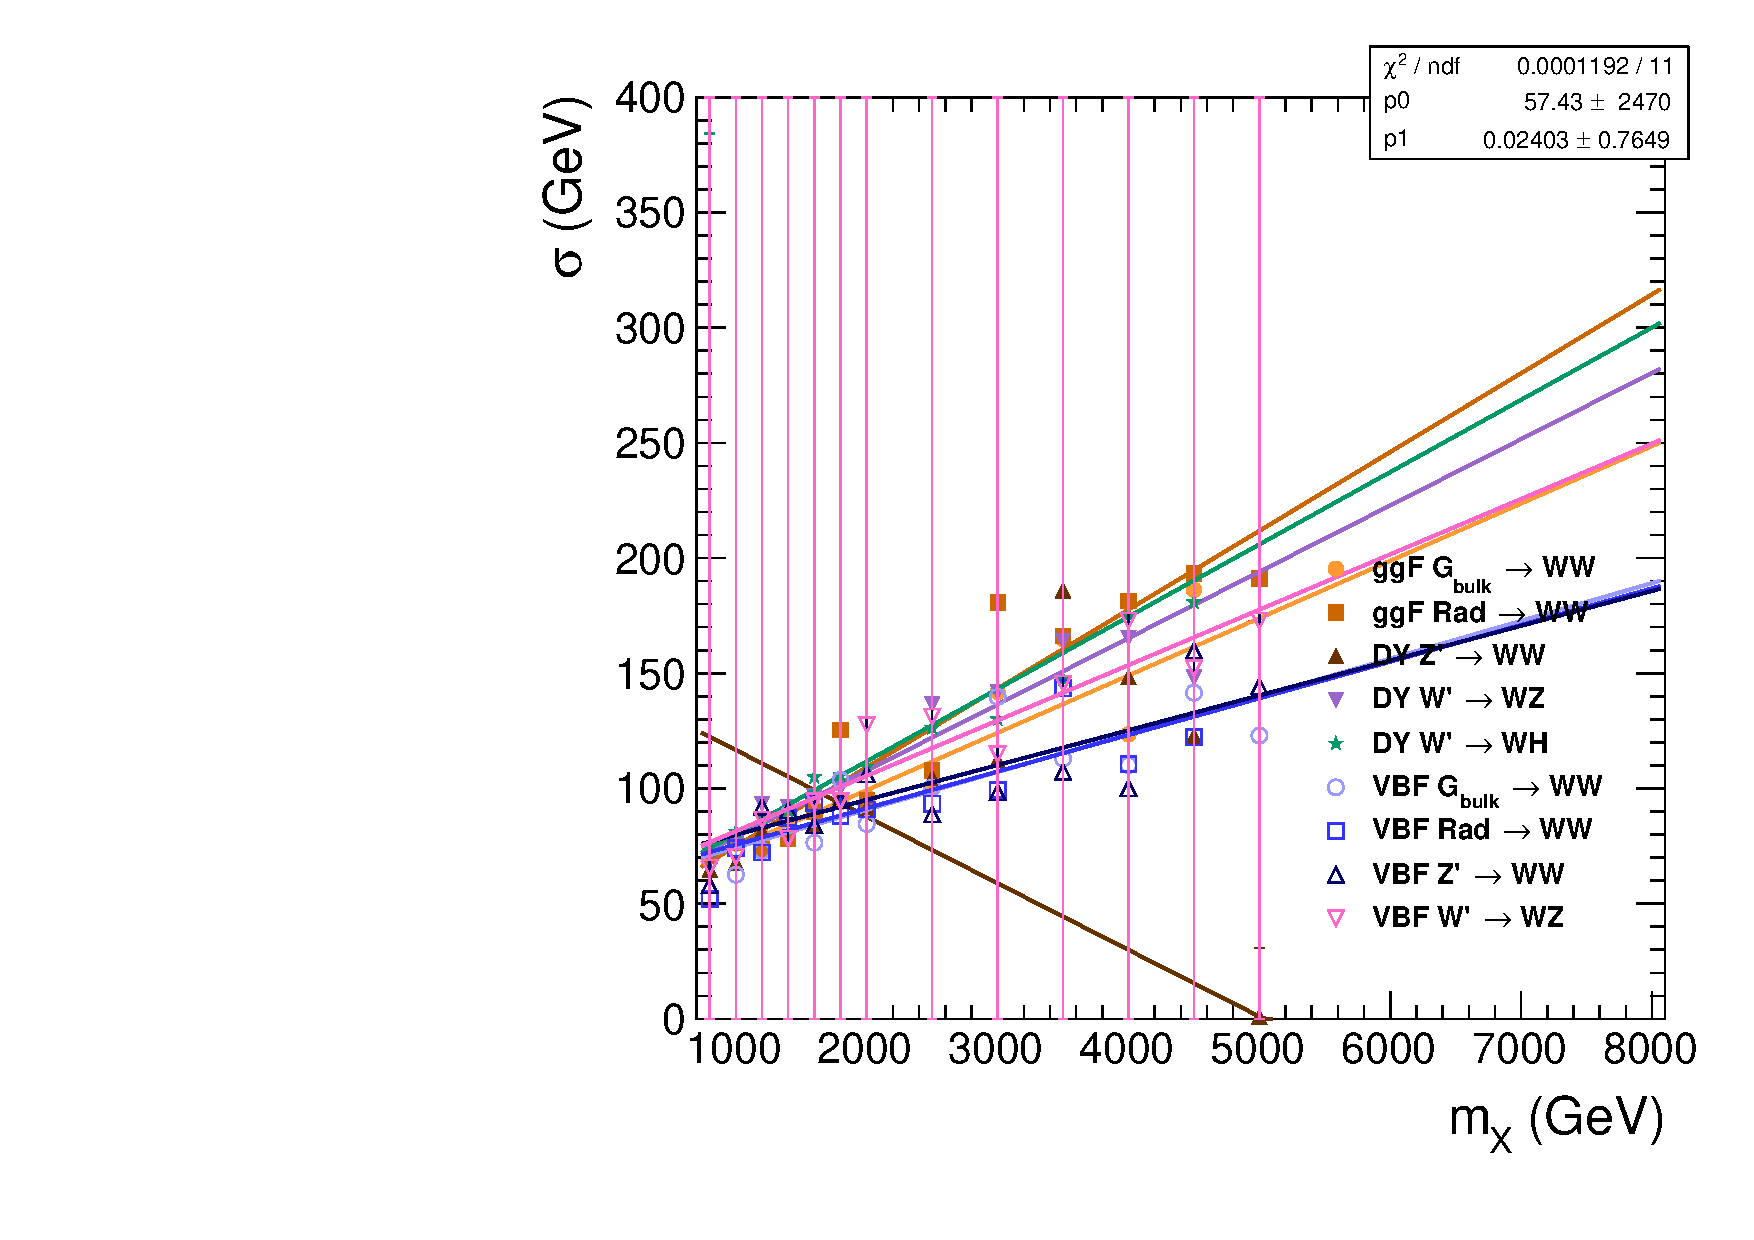
\includegraphics[width=0.2\textwidth]{fig/analysisAppendix/paramSignalShape_allSig_MVV_LP_bb_LDy_SIGMA.pdf}
  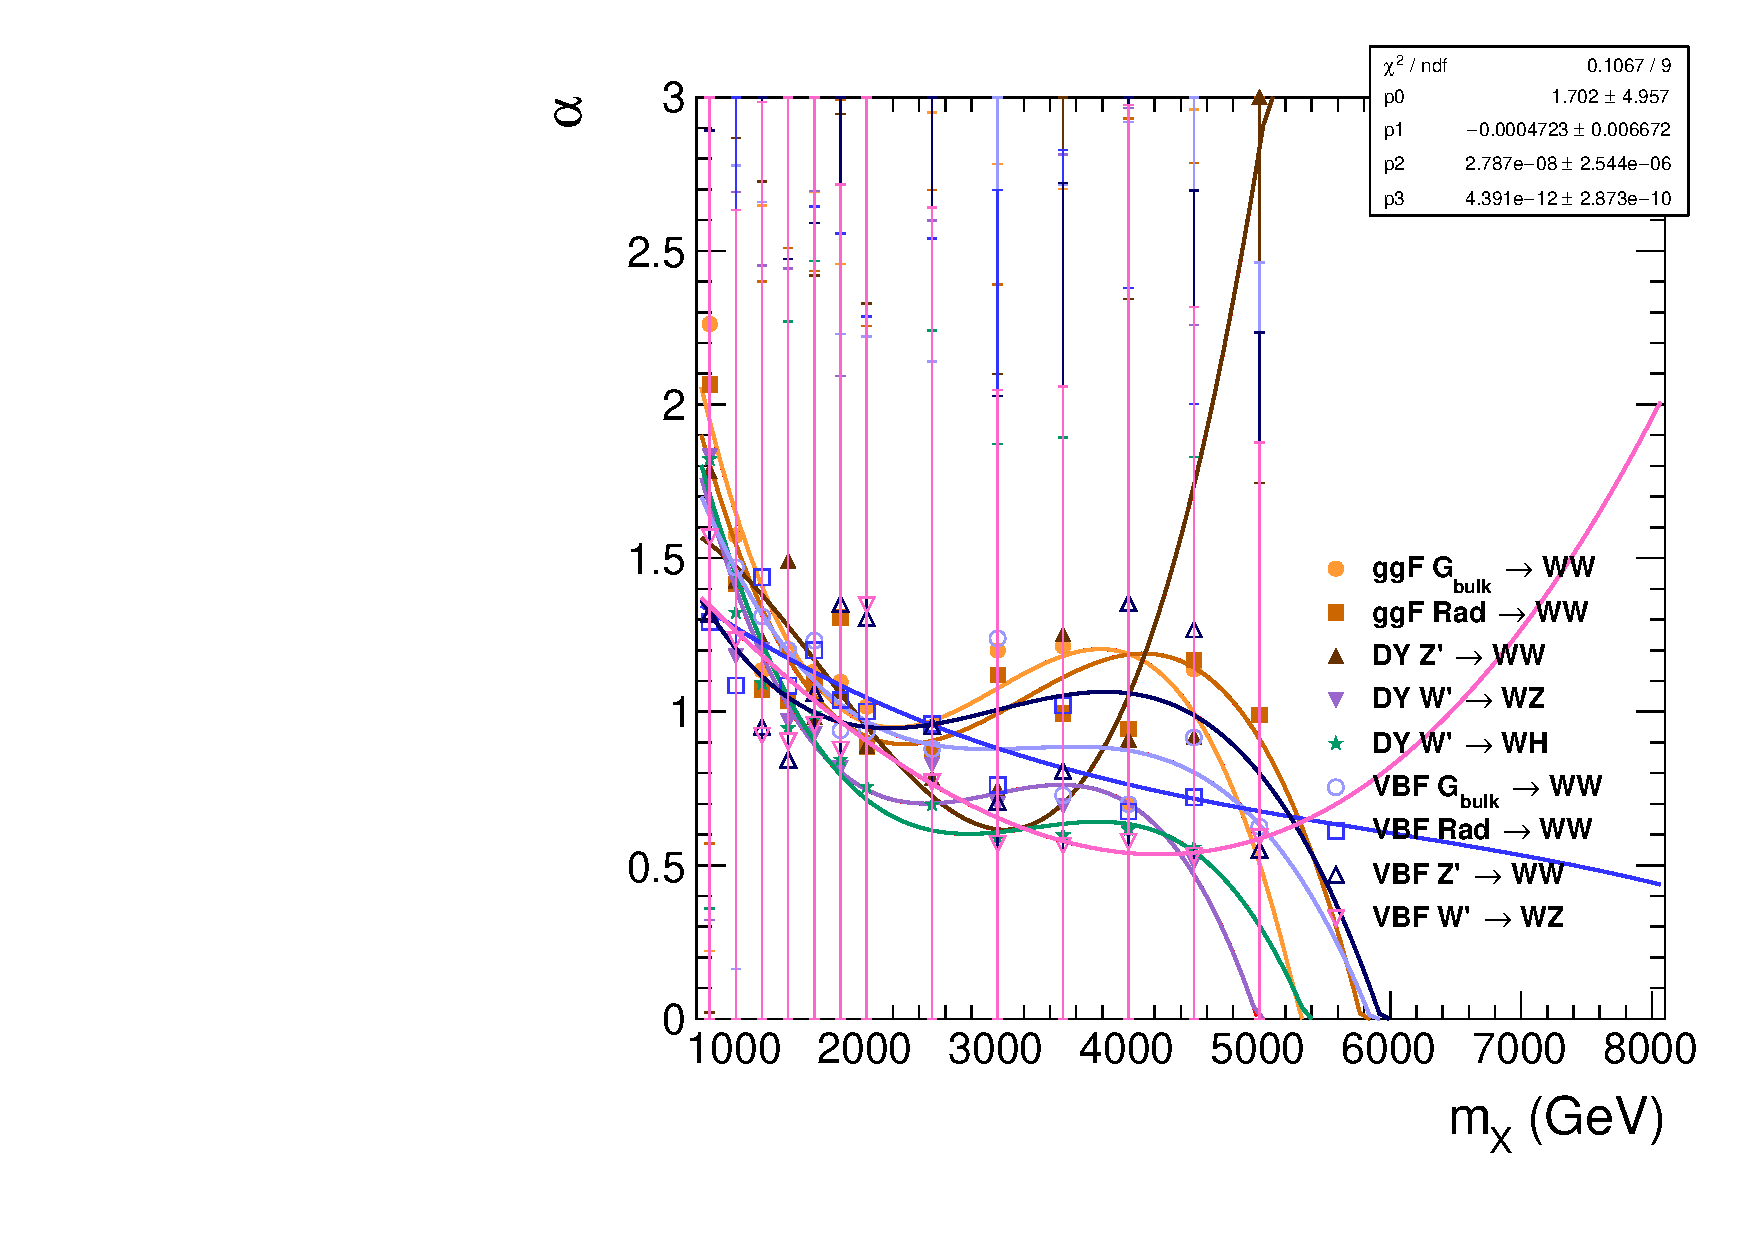
\includegraphics[width=0.2\textwidth]{fig/analysisAppendix/paramSignalShape_allSig_MVV_LP_bb_LDy_ALPHA1.pdf}
  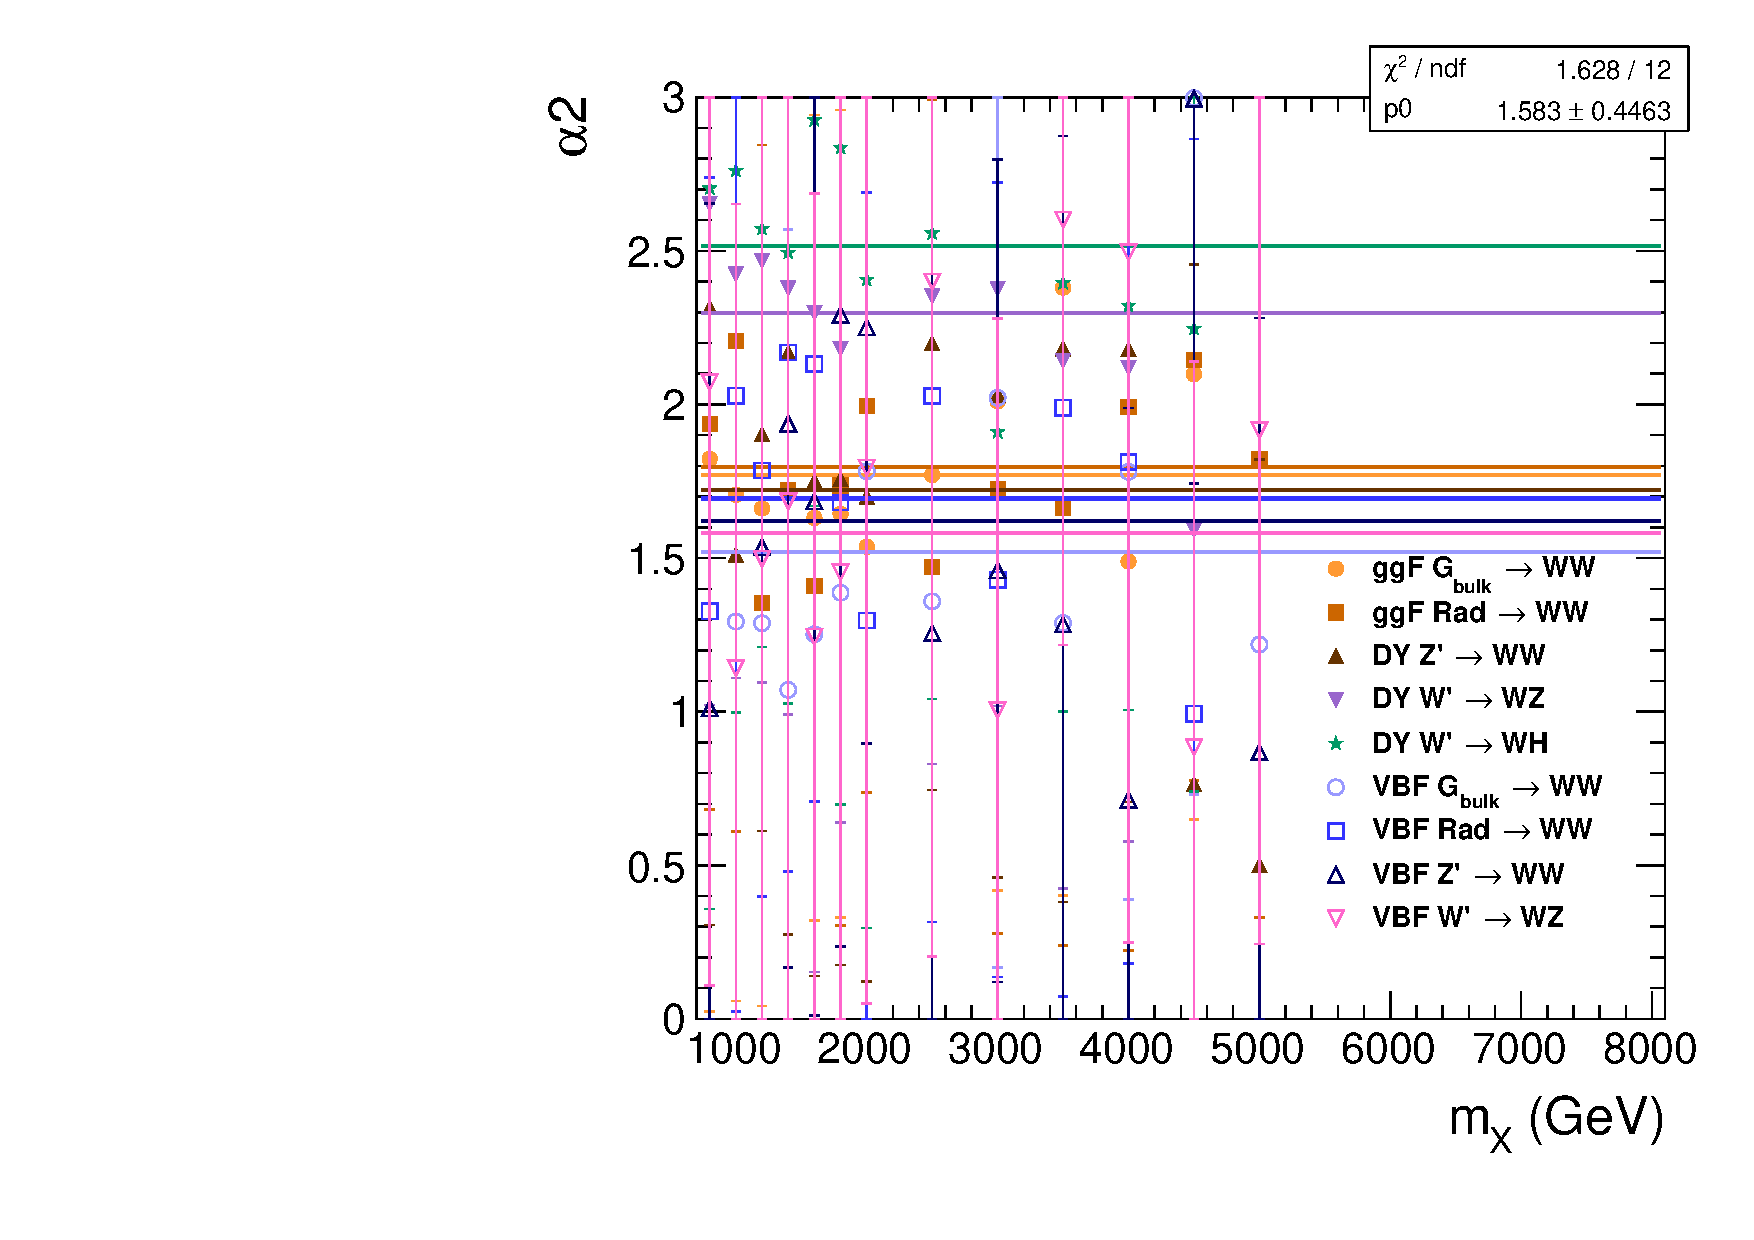
\includegraphics[width=0.2\textwidth]{fig/analysisAppendix/paramSignalShape_allSig_MVV_LP_bb_LDy_ALPHA2.pdf}\\
  \includegraphics[width=0.2\textwidth]{fig/analysisAppendix/paramSignalShape_allSig_MVV_HP_nobb_LDy_MEAN.pdf}
  \includegraphics[width=0.2\textwidth]{fig/analysisAppendix/paramSignalShape_allSig_MVV_HP_nobb_LDy_SIGMA.pdf}
  \includegraphics[width=0.2\textwidth]{fig/analysisAppendix/paramSignalShape_allSig_MVV_HP_nobb_LDy_ALPHA1.pdf}
  \includegraphics[width=0.2\textwidth]{fig/analysisAppendix/paramSignalShape_allSig_MVV_HP_nobb_LDy_ALPHA2.pdf}\\
  \includegraphics[width=0.2\textwidth]{fig/analysisAppendix/paramSignalShape_allSig_MVV_LP_nobb_LDy_MEAN.pdf}
  \includegraphics[width=0.2\textwidth]{fig/analysisAppendix/paramSignalShape_allSig_MVV_LP_nobb_LDy_SIGMA.pdf}
  \includegraphics[width=0.2\textwidth]{fig/analysisAppendix/paramSignalShape_allSig_MVV_LP_nobb_LDy_ALPHA1.pdf}
  \includegraphics[width=0.2\textwidth]{fig/analysisAppendix/paramSignalShape_allSig_MVV_LP_nobb_LDy_ALPHA2.pdf}\\
  \includegraphics[width=0.2\textwidth]{fig/analysisAppendix/paramSignalShape_allSig_MVV_HP_vbf_LDy_MEAN.pdf}
  \includegraphics[width=0.2\textwidth]{fig/analysisAppendix/paramSignalShape_allSig_MVV_HP_vbf_LDy_SIGMA.pdf}
  \includegraphics[width=0.2\textwidth]{fig/analysisAppendix/paramSignalShape_allSig_MVV_HP_vbf_LDy_ALPHA1.pdf}
  \includegraphics[width=0.2\textwidth]{fig/analysisAppendix/paramSignalShape_allSig_MVV_HP_vbf_LDy_ALPHA2.pdf}\\
  \includegraphics[width=0.2\textwidth]{fig/analysisAppendix/paramSignalShape_allSig_MVV_LP_vbf_LDy_MEAN.pdf}
  \includegraphics[width=0.2\textwidth]{fig/analysisAppendix/paramSignalShape_allSig_MVV_LP_vbf_LDy_SIGMA.pdf}
  \includegraphics[width=0.2\textwidth]{fig/analysisAppendix/paramSignalShape_allSig_MVV_LP_vbf_LDy_ALPHA1.pdf}
  \includegraphics[width=0.2\textwidth]{fig/analysisAppendix/paramSignalShape_allSig_MVV_LP_vbf_LDy_ALPHA2.pdf}\\
  \caption{
    DCB parameters (from left to right: $\mu$, $\sigma$, $\alpha_1$, $\alpha_2$) for the diboson reconstructed mass \MVV as a function of \MX.
    Rows 1 to 6: HP-bb-LDy, LP-bb-LDy, HP-nobb-LDy, LP-nobb-LDy, HP-vbf-LDy, LP-vbf-LDy.
  }
  \label{fig:MVVShapeParam_LDy}
\end{figure}

\begin{figure}[htbp]
  \centering
  \includegraphics[width=0.2\textwidth]{fig/analysisAppendix/paramSignalShape_allSig_MVV_HP_bb_HDy_MEAN.pdf}
  \includegraphics[width=0.2\textwidth]{fig/analysisAppendix/paramSignalShape_allSig_MVV_HP_bb_HDy_SIGMA.pdf}
  \includegraphics[width=0.2\textwidth]{fig/analysisAppendix/paramSignalShape_allSig_MVV_HP_bb_HDy_ALPHA1.pdf}
  \includegraphics[width=0.2\textwidth]{fig/analysisAppendix/paramSignalShape_allSig_MVV_HP_bb_HDy_ALPHA2.pdf}\\
  \includegraphics[width=0.2\textwidth]{fig/analysisAppendix/paramSignalShape_allSig_MVV_LP_bb_HDy_MEAN.pdf}
  \includegraphics[width=0.2\textwidth]{fig/analysisAppendix/paramSignalShape_allSig_MVV_LP_bb_HDy_SIGMA.pdf}
  \includegraphics[width=0.2\textwidth]{fig/analysisAppendix/paramSignalShape_allSig_MVV_LP_bb_HDy_ALPHA1.pdf}
  \includegraphics[width=0.2\textwidth]{fig/analysisAppendix/paramSignalShape_allSig_MVV_LP_bb_HDy_ALPHA2.pdf}\\
  \includegraphics[width=0.2\textwidth]{fig/analysisAppendix/paramSignalShape_allSig_MVV_HP_nobb_HDy_MEAN.pdf}
  \includegraphics[width=0.2\textwidth]{fig/analysisAppendix/paramSignalShape_allSig_MVV_HP_nobb_HDy_SIGMA.pdf}
  \includegraphics[width=0.2\textwidth]{fig/analysisAppendix/paramSignalShape_allSig_MVV_HP_nobb_HDy_ALPHA1.pdf}
  \includegraphics[width=0.2\textwidth]{fig/analysisAppendix/paramSignalShape_allSig_MVV_HP_nobb_HDy_ALPHA2.pdf}\\
  \includegraphics[width=0.2\textwidth]{fig/analysisAppendix/paramSignalShape_allSig_MVV_LP_nobb_HDy_MEAN.pdf}
  \includegraphics[width=0.2\textwidth]{fig/analysisAppendix/paramSignalShape_allSig_MVV_LP_nobb_HDy_SIGMA.pdf}
  \includegraphics[width=0.2\textwidth]{fig/analysisAppendix/paramSignalShape_allSig_MVV_LP_nobb_HDy_ALPHA1.pdf}
  \includegraphics[width=0.2\textwidth]{fig/analysisAppendix/paramSignalShape_allSig_MVV_LP_nobb_HDy_ALPHA2.pdf}\\
  \includegraphics[width=0.2\textwidth]{fig/analysisAppendix/paramSignalShape_allSig_MVV_HP_vbf_HDy_MEAN.pdf}
  \includegraphics[width=0.2\textwidth]{fig/analysisAppendix/paramSignalShape_allSig_MVV_HP_vbf_HDy_SIGMA.pdf}
  \includegraphics[width=0.2\textwidth]{fig/analysisAppendix/paramSignalShape_allSig_MVV_HP_vbf_HDy_ALPHA1.pdf}
  \includegraphics[width=0.2\textwidth]{fig/analysisAppendix/paramSignalShape_allSig_MVV_HP_vbf_HDy_ALPHA2.pdf}\\
  \includegraphics[width=0.2\textwidth]{fig/analysisAppendix/paramSignalShape_allSig_MVV_LP_vbf_HDy_MEAN.pdf}
  \includegraphics[width=0.2\textwidth]{fig/analysisAppendix/paramSignalShape_allSig_MVV_LP_vbf_HDy_SIGMA.pdf}
  \includegraphics[width=0.2\textwidth]{fig/analysisAppendix/paramSignalShape_allSig_MVV_LP_vbf_HDy_ALPHA1.pdf}
  \includegraphics[width=0.2\textwidth]{fig/analysisAppendix/paramSignalShape_allSig_MVV_LP_vbf_HDy_ALPHA2.pdf}\\
  \caption{
    DCB parameters (from left to right: $\mu$, $\sigma$, $\alpha_1$, $\alpha_2$) for the diboson reconstructed mass \MVV as a function of \MX.
    Rows 1 to 6: HP-bb-HDy, LP-bb-HDy, HP-nobb-HDy, LP-nobb-HDy, HP-vbf-HDy, LP-vbf-HDy.
  }
  \label{fig:MVVShapeParam_HDy}
\end{figure}

\begin{figure}[htbp]
  \centering
  \includegraphics[width=0.2\textwidth]{fig/analysisAppendix/paramSignalShape_allSig_MJJ_HP_bb_LDy_mean.pdf}
  \includegraphics[width=0.2\textwidth]{fig/analysisAppendix/paramSignalShape_allSig_MJJ_HP_bb_LDy_sigma.pdf}
  \includegraphics[width=0.2\textwidth]{fig/analysisAppendix/paramSignalShape_allSig_MJJ_HP_bb_LDy_alpha.pdf}
  \includegraphics[width=0.2\textwidth]{fig/analysisAppendix/paramSignalShape_allSig_MJJ_HP_bb_LDy_alpha2.pdf}\\
  \includegraphics[width=0.2\textwidth]{fig/analysisAppendix/paramSignalShape_allSig_MJJ_LP_bb_LDy_mean.pdf}
  \includegraphics[width=0.2\textwidth]{fig/analysisAppendix/paramSignalShape_allSig_MJJ_LP_bb_LDy_sigma.pdf}
  \includegraphics[width=0.2\textwidth]{fig/analysisAppendix/paramSignalShape_allSig_MJJ_LP_bb_LDy_alpha.pdf}
  \includegraphics[width=0.2\textwidth]{fig/analysisAppendix/paramSignalShape_allSig_MJJ_LP_bb_LDy_alpha2.pdf}\\
  \includegraphics[width=0.2\textwidth]{fig/analysisAppendix/paramSignalShape_allSig_MJJ_HP_nobb_LDy_mean.pdf}
  \includegraphics[width=0.2\textwidth]{fig/analysisAppendix/paramSignalShape_allSig_MJJ_HP_nobb_LDy_sigma.pdf}
  \includegraphics[width=0.2\textwidth]{fig/analysisAppendix/paramSignalShape_allSig_MJJ_HP_nobb_LDy_alpha.pdf}
  \includegraphics[width=0.2\textwidth]{fig/analysisAppendix/paramSignalShape_allSig_MJJ_HP_nobb_LDy_alpha2.pdf}\\
  \includegraphics[width=0.2\textwidth]{fig/analysisAppendix/paramSignalShape_allSig_MJJ_LP_nobb_LDy_mean.pdf}
  \includegraphics[width=0.2\textwidth]{fig/analysisAppendix/paramSignalShape_allSig_MJJ_LP_nobb_LDy_sigma.pdf}
  \includegraphics[width=0.2\textwidth]{fig/analysisAppendix/paramSignalShape_allSig_MJJ_LP_nobb_LDy_alpha.pdf}
  \includegraphics[width=0.2\textwidth]{fig/analysisAppendix/paramSignalShape_allSig_MJJ_LP_nobb_LDy_alpha2.pdf}\\
  \includegraphics[width=0.2\textwidth]{fig/analysisAppendix/paramSignalShape_allSig_MJJ_HP_vbf_LDy_mean.pdf}
  \includegraphics[width=0.2\textwidth]{fig/analysisAppendix/paramSignalShape_allSig_MJJ_HP_vbf_LDy_sigma.pdf}
  \includegraphics[width=0.2\textwidth]{fig/analysisAppendix/paramSignalShape_allSig_MJJ_HP_vbf_LDy_alpha.pdf}
  \includegraphics[width=0.2\textwidth]{fig/analysisAppendix/paramSignalShape_allSig_MJJ_HP_vbf_LDy_alpha2.pdf}\\
  \includegraphics[width=0.2\textwidth]{fig/analysisAppendix/paramSignalShape_allSig_MJJ_LP_vbf_LDy_mean.pdf}
  \includegraphics[width=0.2\textwidth]{fig/analysisAppendix/paramSignalShape_allSig_MJJ_LP_vbf_LDy_sigma.pdf}
  \includegraphics[width=0.2\textwidth]{fig/analysisAppendix/paramSignalShape_allSig_MJJ_LP_vbf_LDy_alpha.pdf}
  \includegraphics[width=0.2\textwidth]{fig/analysisAppendix/paramSignalShape_allSig_MJJ_LP_vbf_LDy_alpha2.pdf}\\
  \caption{
    DCB parameters (from left to right: $\mu$, $\sigma$, $\alpha_1$, $\alpha_2$) for the jet mass \MJ as a function of \MX.
    Rows 1 to 6: HP-bb-LDy, LP-bb-LDy, HP-nobb-LDy, LP-nobb-LDy, HP-vbf-LDy, LP-vbf-LDy.
  }
  \label{fig:MJJShapeParam_LDy}
\end{figure}

\begin{figure}[htbp]
  \centering
  \includegraphics[width=0.2\textwidth]{fig/analysisAppendix/paramSignalShape_allSig_MJJ_HP_bb_HDy_mean.pdf}
  \includegraphics[width=0.2\textwidth]{fig/analysisAppendix/paramSignalShape_allSig_MJJ_HP_bb_HDy_sigma.pdf}
  \includegraphics[width=0.2\textwidth]{fig/analysisAppendix/paramSignalShape_allSig_MJJ_HP_bb_HDy_alpha.pdf}
  \includegraphics[width=0.2\textwidth]{fig/analysisAppendix/paramSignalShape_allSig_MJJ_HP_bb_HDy_alpha2.pdf}\\
  \includegraphics[width=0.2\textwidth]{fig/analysisAppendix/paramSignalShape_allSig_MJJ_LP_bb_HDy_mean.pdf}
  \includegraphics[width=0.2\textwidth]{fig/analysisAppendix/paramSignalShape_allSig_MJJ_LP_bb_HDy_sigma.pdf}
  \includegraphics[width=0.2\textwidth]{fig/analysisAppendix/paramSignalShape_allSig_MJJ_LP_bb_HDy_alpha.pdf}
  \includegraphics[width=0.2\textwidth]{fig/analysisAppendix/paramSignalShape_allSig_MJJ_LP_bb_HDy_alpha2.pdf}\\
  \includegraphics[width=0.2\textwidth]{fig/analysisAppendix/paramSignalShape_allSig_MJJ_HP_nobb_HDy_mean.pdf}
  \includegraphics[width=0.2\textwidth]{fig/analysisAppendix/paramSignalShape_allSig_MJJ_HP_nobb_HDy_sigma.pdf}
  \includegraphics[width=0.2\textwidth]{fig/analysisAppendix/paramSignalShape_allSig_MJJ_HP_nobb_HDy_alpha.pdf}
  \includegraphics[width=0.2\textwidth]{fig/analysisAppendix/paramSignalShape_allSig_MJJ_HP_nobb_HDy_alpha2.pdf}\\
  \includegraphics[width=0.2\textwidth]{fig/analysisAppendix/paramSignalShape_allSig_MJJ_LP_nobb_HDy_mean.pdf}
  \includegraphics[width=0.2\textwidth]{fig/analysisAppendix/paramSignalShape_allSig_MJJ_LP_nobb_HDy_sigma.pdf}
  \includegraphics[width=0.2\textwidth]{fig/analysisAppendix/paramSignalShape_allSig_MJJ_LP_nobb_HDy_alpha.pdf}
  \includegraphics[width=0.2\textwidth]{fig/analysisAppendix/paramSignalShape_allSig_MJJ_LP_nobb_HDy_alpha2.pdf}\\
  \includegraphics[width=0.2\textwidth]{fig/analysisAppendix/paramSignalShape_allSig_MJJ_HP_vbf_HDy_mean.pdf}
  \includegraphics[width=0.2\textwidth]{fig/analysisAppendix/paramSignalShape_allSig_MJJ_HP_vbf_HDy_sigma.pdf}
  \includegraphics[width=0.2\textwidth]{fig/analysisAppendix/paramSignalShape_allSig_MJJ_HP_vbf_HDy_alpha.pdf}
  \includegraphics[width=0.2\textwidth]{fig/analysisAppendix/paramSignalShape_allSig_MJJ_HP_vbf_HDy_alpha2.pdf}\\
  \includegraphics[width=0.2\textwidth]{fig/analysisAppendix/paramSignalShape_allSig_MJJ_LP_vbf_HDy_mean.pdf}
  \includegraphics[width=0.2\textwidth]{fig/analysisAppendix/paramSignalShape_allSig_MJJ_LP_vbf_HDy_sigma.pdf}
  \includegraphics[width=0.2\textwidth]{fig/analysisAppendix/paramSignalShape_allSig_MJJ_LP_vbf_HDy_alpha.pdf}
  \includegraphics[width=0.2\textwidth]{fig/analysisAppendix/paramSignalShape_allSig_MJJ_LP_vbf_HDy_alpha2.pdf}\\
  \caption{
    DCB parameters (from left to right: $\mu$, $\sigma$, $\alpha_1$, $\alpha_2$) for the jet mass \MJ as a function of \MX.
    Rows 1 to 6: HP-bb-HDy, LP-bb-HDy, HP-nobb-HDy, LP-nobb-HDy, HP-vbf-HDy, LP-vbf-HDy.
  }
  \label{fig:MJJShapeParam_HDy}
\end{figure}

\begin{figure}[htbp]
  \centering
  \includegraphics[width=0.18\textwidth]{fig/analysisAppendix/templateSignalVsMX_fromDC_GbuToWW_MVV_mu_HP_bb_LDy.pdf}
  \includegraphics[width=0.18\textwidth]{fig/analysisAppendix/templateSignalVsMX_fromDC_RadToWW_MVV_mu_HP_bb_LDy.pdf}
  \includegraphics[width=0.18\textwidth]{fig/analysisAppendix/templateSignalVsMX_fromDC_ZprToWW_MVV_mu_HP_bb_LDy.pdf}
  \includegraphics[width=0.18\textwidth]{fig/analysisAppendix/templateSignalVsMX_fromDC_WprToWZ_MVV_mu_HP_bb_LDy.pdf}
  \includegraphics[width=0.18\textwidth]{fig/analysisAppendix/templateSignalVsMX_fromDC_WprToWH_MVV_mu_HP_bb_LDy.pdf}\\
  \includegraphics[width=0.18\textwidth]{fig/analysisAppendix/templateSignalVsMX_fromDC_GbuToWW_MVV_mu_LP_bb_LDy.pdf}
  \includegraphics[width=0.18\textwidth]{fig/analysisAppendix/templateSignalVsMX_fromDC_RadToWW_MVV_mu_LP_bb_LDy.pdf}
  \includegraphics[width=0.18\textwidth]{fig/analysisAppendix/templateSignalVsMX_fromDC_ZprToWW_MVV_mu_LP_bb_LDy.pdf}
  \includegraphics[width=0.18\textwidth]{fig/analysisAppendix/templateSignalVsMX_fromDC_WprToWZ_MVV_mu_LP_bb_LDy.pdf}
  \includegraphics[width=0.18\textwidth]{fig/analysisAppendix/templateSignalVsMX_fromDC_WprToWH_MVV_mu_LP_bb_LDy.pdf}\\
  \includegraphics[width=0.18\textwidth]{fig/analysisAppendix/templateSignalVsMX_fromDC_GbuToWW_MVV_mu_HP_nobb_LDy.pdf}
  \includegraphics[width=0.18\textwidth]{fig/analysisAppendix/templateSignalVsMX_fromDC_RadToWW_MVV_mu_HP_nobb_LDy.pdf}
  \includegraphics[width=0.18\textwidth]{fig/analysisAppendix/templateSignalVsMX_fromDC_ZprToWW_MVV_mu_HP_nobb_LDy.pdf}
  \includegraphics[width=0.18\textwidth]{fig/analysisAppendix/templateSignalVsMX_fromDC_WprToWZ_MVV_mu_HP_nobb_LDy.pdf}
  \includegraphics[width=0.18\textwidth]{fig/analysisAppendix/templateSignalVsMX_fromDC_WprToWH_MVV_mu_HP_nobb_LDy.pdf}\\
  \includegraphics[width=0.18\textwidth]{fig/analysisAppendix/templateSignalVsMX_fromDC_GbuToWW_MVV_mu_LP_nobb_LDy.pdf}
  \includegraphics[width=0.18\textwidth]{fig/analysisAppendix/templateSignalVsMX_fromDC_RadToWW_MVV_mu_LP_nobb_LDy.pdf}
  \includegraphics[width=0.18\textwidth]{fig/analysisAppendix/templateSignalVsMX_fromDC_ZprToWW_MVV_mu_LP_nobb_LDy.pdf}
  \includegraphics[width=0.18\textwidth]{fig/analysisAppendix/templateSignalVsMX_fromDC_WprToWZ_MVV_mu_LP_nobb_LDy.pdf}
  \includegraphics[width=0.18\textwidth]{fig/analysisAppendix/templateSignalVsMX_fromDC_WprToWH_MVV_mu_LP_nobb_LDy.pdf}\\
  \includegraphics[width=0.18\textwidth]{fig/analysisAppendix/templateSignalVsMX_fromDC_GbuToWW_MVV_mu_HP_vbf_LDy.pdf}
  \includegraphics[width=0.18\textwidth]{fig/analysisAppendix/templateSignalVsMX_fromDC_RadToWW_MVV_mu_HP_vbf_LDy.pdf}
  \includegraphics[width=0.18\textwidth]{fig/analysisAppendix/templateSignalVsMX_fromDC_ZprToWW_MVV_mu_HP_vbf_LDy.pdf}
  \includegraphics[width=0.18\textwidth]{fig/analysisAppendix/templateSignalVsMX_fromDC_WprToWZ_MVV_mu_HP_vbf_LDy.pdf}
  \includegraphics[width=0.18\textwidth]{fig/analysisAppendix/templateSignalVsMX_fromDC_WprToWH_MVV_mu_HP_vbf_LDy.pdf}\\
  \includegraphics[width=0.18\textwidth]{fig/analysisAppendix/templateSignalVsMX_fromDC_GbuToWW_MVV_mu_LP_vbf_LDy.pdf}
  \includegraphics[width=0.18\textwidth]{fig/analysisAppendix/templateSignalVsMX_fromDC_RadToWW_MVV_mu_LP_vbf_LDy.pdf}
  \includegraphics[width=0.18\textwidth]{fig/analysisAppendix/templateSignalVsMX_fromDC_ZprToWW_MVV_mu_LP_vbf_LDy.pdf}
  \includegraphics[width=0.18\textwidth]{fig/analysisAppendix/templateSignalVsMX_fromDC_WprToWZ_MVV_mu_LP_vbf_LDy.pdf}
  \includegraphics[width=0.18\textwidth]{fig/analysisAppendix/templateSignalVsMX_fromDC_WprToWH_MVV_mu_LP_vbf_LDy.pdf}\\
  \caption{
    Signal shapes for the diboson reconstructed mass \MVV for \ggF- and \DY-produced signals, for 8 values of \MX.
    From left to right: \GBulktoWW, \RadtoWW, \ZprtoWW, \WprtoWZ, \WprtoWH.
    Rows 1 to 6: HP-bb-LDy, LP-bb-LDy, HP-nobb-LDy, LP-nobb-LDy, HP-vbf-LDy, LP-vbf-LDy.
  }
  \label{fig:MVVShapes_NonVBF_LDy}
\end{figure}

\begin{figure}[htbp]
  \centering
  \includegraphics[width=0.18\textwidth]{fig/analysisAppendix/templateSignalVsMX_fromDC_GbuToWW_MVV_mu_HP_bb_HDy.pdf}
  \includegraphics[width=0.18\textwidth]{fig/analysisAppendix/templateSignalVsMX_fromDC_RadToWW_MVV_mu_HP_bb_HDy.pdf}
  \includegraphics[width=0.18\textwidth]{fig/analysisAppendix/templateSignalVsMX_fromDC_ZprToWW_MVV_mu_HP_bb_HDy.pdf}
  \includegraphics[width=0.18\textwidth]{fig/analysisAppendix/templateSignalVsMX_fromDC_WprToWZ_MVV_mu_HP_bb_HDy.pdf}
  \includegraphics[width=0.18\textwidth]{fig/analysisAppendix/templateSignalVsMX_fromDC_WprToWH_MVV_mu_HP_bb_HDy.pdf}\\
  \includegraphics[width=0.18\textwidth]{fig/analysisAppendix/templateSignalVsMX_fromDC_GbuToWW_MVV_mu_LP_bb_HDy.pdf}
  \includegraphics[width=0.18\textwidth]{fig/analysisAppendix/templateSignalVsMX_fromDC_RadToWW_MVV_mu_LP_bb_HDy.pdf}
  \includegraphics[width=0.18\textwidth]{fig/analysisAppendix/templateSignalVsMX_fromDC_ZprToWW_MVV_mu_LP_bb_HDy.pdf}
  \includegraphics[width=0.18\textwidth]{fig/analysisAppendix/templateSignalVsMX_fromDC_WprToWZ_MVV_mu_LP_bb_HDy.pdf}
  \includegraphics[width=0.18\textwidth]{fig/analysisAppendix/templateSignalVsMX_fromDC_WprToWH_MVV_mu_LP_bb_HDy.pdf}\\
  \includegraphics[width=0.18\textwidth]{fig/analysisAppendix/templateSignalVsMX_fromDC_GbuToWW_MVV_mu_HP_nobb_HDy.pdf}
  \includegraphics[width=0.18\textwidth]{fig/analysisAppendix/templateSignalVsMX_fromDC_RadToWW_MVV_mu_HP_nobb_HDy.pdf}
  \includegraphics[width=0.18\textwidth]{fig/analysisAppendix/templateSignalVsMX_fromDC_ZprToWW_MVV_mu_HP_nobb_HDy.pdf}
  \includegraphics[width=0.18\textwidth]{fig/analysisAppendix/templateSignalVsMX_fromDC_WprToWZ_MVV_mu_HP_nobb_HDy.pdf}
  \includegraphics[width=0.18\textwidth]{fig/analysisAppendix/templateSignalVsMX_fromDC_WprToWH_MVV_mu_HP_nobb_HDy.pdf}\\
  \includegraphics[width=0.18\textwidth]{fig/analysisAppendix/templateSignalVsMX_fromDC_GbuToWW_MVV_mu_LP_nobb_HDy.pdf}
  \includegraphics[width=0.18\textwidth]{fig/analysisAppendix/templateSignalVsMX_fromDC_RadToWW_MVV_mu_LP_nobb_HDy.pdf}
  \includegraphics[width=0.18\textwidth]{fig/analysisAppendix/templateSignalVsMX_fromDC_ZprToWW_MVV_mu_LP_nobb_HDy.pdf}
  \includegraphics[width=0.18\textwidth]{fig/analysisAppendix/templateSignalVsMX_fromDC_WprToWZ_MVV_mu_LP_nobb_HDy.pdf}
  \includegraphics[width=0.18\textwidth]{fig/analysisAppendix/templateSignalVsMX_fromDC_WprToWH_MVV_mu_LP_nobb_HDy.pdf}\\
  \includegraphics[width=0.18\textwidth]{fig/analysisAppendix/templateSignalVsMX_fromDC_GbuToWW_MVV_mu_HP_vbf_HDy.pdf}
  \includegraphics[width=0.18\textwidth]{fig/analysisAppendix/templateSignalVsMX_fromDC_RadToWW_MVV_mu_HP_vbf_HDy.pdf}
  \includegraphics[width=0.18\textwidth]{fig/analysisAppendix/templateSignalVsMX_fromDC_ZprToWW_MVV_mu_HP_vbf_HDy.pdf}
  \includegraphics[width=0.18\textwidth]{fig/analysisAppendix/templateSignalVsMX_fromDC_WprToWZ_MVV_mu_HP_vbf_HDy.pdf}
  \includegraphics[width=0.18\textwidth]{fig/analysisAppendix/templateSignalVsMX_fromDC_WprToWH_MVV_mu_HP_vbf_HDy.pdf}\\
  \includegraphics[width=0.18\textwidth]{fig/analysisAppendix/templateSignalVsMX_fromDC_GbuToWW_MVV_mu_LP_vbf_HDy.pdf}
  \includegraphics[width=0.18\textwidth]{fig/analysisAppendix/templateSignalVsMX_fromDC_RadToWW_MVV_mu_LP_vbf_HDy.pdf}
  \includegraphics[width=0.18\textwidth]{fig/analysisAppendix/templateSignalVsMX_fromDC_ZprToWW_MVV_mu_LP_vbf_HDy.pdf}
  \includegraphics[width=0.18\textwidth]{fig/analysisAppendix/templateSignalVsMX_fromDC_WprToWZ_MVV_mu_LP_vbf_HDy.pdf}
  \includegraphics[width=0.18\textwidth]{fig/analysisAppendix/templateSignalVsMX_fromDC_WprToWH_MVV_mu_LP_vbf_HDy.pdf}\\
  \caption{
    Signal shapes for the diboson reconstructed mass \MVV for \ggF- and \DY-produced signals, for 8 values of \MX.
    From left to right: \GBulktoWW, \RadtoWW, \ZprtoWW, \WprtoWZ, \WprtoWH.
    Rows 1 to 6: HP-bb-HDy, LP-bb-HDy, HP-nobb-HDy, LP-nobb-HDy, HP-vbf-HDy, LP-vbf-HDy.
  }
  \label{fig:MVVShapes_NonVBF_HDy}
\end{figure}

\begin{figure}[htbp]
  \centering
  \includegraphics[width=0.18\textwidth]{fig/analysisAppendix/templateSignalVsMX_fromDC_VBFGbuToWW_MVV_mu_HP_bb_LDy.pdf}
  \includegraphics[width=0.18\textwidth]{fig/analysisAppendix/templateSignalVsMX_fromDC_VBFRadToWW_MVV_mu_HP_bb_LDy.pdf}
  \includegraphics[width=0.18\textwidth]{fig/analysisAppendix/templateSignalVsMX_fromDC_VBFZprToWW_MVV_mu_HP_bb_LDy.pdf}
  \includegraphics[width=0.18\textwidth]{fig/analysisAppendix/templateSignalVsMX_fromDC_VBFWprToWZ_MVV_mu_HP_bb_LDy.pdf}\\
  \includegraphics[width=0.18\textwidth]{fig/analysisAppendix/templateSignalVsMX_fromDC_VBFGbuToWW_MVV_mu_LP_bb_LDy.pdf}
  \includegraphics[width=0.18\textwidth]{fig/analysisAppendix/templateSignalVsMX_fromDC_VBFRadToWW_MVV_mu_LP_bb_LDy.pdf}
  \includegraphics[width=0.18\textwidth]{fig/analysisAppendix/templateSignalVsMX_fromDC_VBFZprToWW_MVV_mu_LP_bb_LDy.pdf}
  \includegraphics[width=0.18\textwidth]{fig/analysisAppendix/templateSignalVsMX_fromDC_VBFWprToWZ_MVV_mu_LP_bb_LDy.pdf}\\
  \includegraphics[width=0.18\textwidth]{fig/analysisAppendix/templateSignalVsMX_fromDC_VBFGbuToWW_MVV_mu_HP_nobb_LDy.pdf}
  \includegraphics[width=0.18\textwidth]{fig/analysisAppendix/templateSignalVsMX_fromDC_VBFRadToWW_MVV_mu_HP_nobb_LDy.pdf}
  \includegraphics[width=0.18\textwidth]{fig/analysisAppendix/templateSignalVsMX_fromDC_VBFZprToWW_MVV_mu_HP_nobb_LDy.pdf}
  \includegraphics[width=0.18\textwidth]{fig/analysisAppendix/templateSignalVsMX_fromDC_VBFWprToWZ_MVV_mu_HP_nobb_LDy.pdf}\\
  \includegraphics[width=0.18\textwidth]{fig/analysisAppendix/templateSignalVsMX_fromDC_VBFGbuToWW_MVV_mu_LP_nobb_LDy.pdf}
  \includegraphics[width=0.18\textwidth]{fig/analysisAppendix/templateSignalVsMX_fromDC_VBFRadToWW_MVV_mu_LP_nobb_LDy.pdf}
  \includegraphics[width=0.18\textwidth]{fig/analysisAppendix/templateSignalVsMX_fromDC_VBFZprToWW_MVV_mu_LP_nobb_LDy.pdf}
  \includegraphics[width=0.18\textwidth]{fig/analysisAppendix/templateSignalVsMX_fromDC_VBFWprToWZ_MVV_mu_LP_nobb_LDy.pdf}\\
  \includegraphics[width=0.18\textwidth]{fig/analysisAppendix/templateSignalVsMX_fromDC_VBFGbuToWW_MVV_mu_HP_vbf_LDy.pdf}
  \includegraphics[width=0.18\textwidth]{fig/analysisAppendix/templateSignalVsMX_fromDC_VBFRadToWW_MVV_mu_HP_vbf_LDy.pdf}
  \includegraphics[width=0.18\textwidth]{fig/analysisAppendix/templateSignalVsMX_fromDC_VBFZprToWW_MVV_mu_HP_vbf_LDy.pdf}
  \includegraphics[width=0.18\textwidth]{fig/analysisAppendix/templateSignalVsMX_fromDC_VBFWprToWZ_MVV_mu_HP_vbf_LDy.pdf}\\
  \includegraphics[width=0.18\textwidth]{fig/analysisAppendix/templateSignalVsMX_fromDC_VBFGbuToWW_MVV_mu_LP_vbf_LDy.pdf}
  \includegraphics[width=0.18\textwidth]{fig/analysisAppendix/templateSignalVsMX_fromDC_VBFRadToWW_MVV_mu_LP_vbf_LDy.pdf}
  \includegraphics[width=0.18\textwidth]{fig/analysisAppendix/templateSignalVsMX_fromDC_VBFZprToWW_MVV_mu_LP_vbf_LDy.pdf}
  \includegraphics[width=0.18\textwidth]{fig/analysisAppendix/templateSignalVsMX_fromDC_VBFWprToWZ_MVV_mu_LP_vbf_LDy.pdf}\\
  \caption{
    Signal shapes for the diboson reconstructed mass \MVV for \VBF-produced signals, for 8 values of \MX.
    From left to right: \GBulktoWW, \RadtoWW, \ZprtoWW, \WprtoWZ.
    Rows 1 to 6: HP-bb-LDy, LP-bb-LDy, HP-nobb-LDy, LP-nobb-LDy, HP-vbf-LDy, LP-vbf-LDy.
  }
  \label{fig:MVVShapes_VBF_LDy}
\end{figure}

\begin{figure}[htbp]
  \centering
  \includegraphics[width=0.18\textwidth]{fig/analysisAppendix/templateSignalVsMX_fromDC_VBFGbuToWW_MVV_mu_HP_bb_HDy.pdf}
  \includegraphics[width=0.18\textwidth]{fig/analysisAppendix/templateSignalVsMX_fromDC_VBFRadToWW_MVV_mu_HP_bb_HDy.pdf}
  \includegraphics[width=0.18\textwidth]{fig/analysisAppendix/templateSignalVsMX_fromDC_VBFZprToWW_MVV_mu_HP_bb_HDy.pdf}
  \includegraphics[width=0.18\textwidth]{fig/analysisAppendix/templateSignalVsMX_fromDC_VBFWprToWZ_MVV_mu_HP_bb_HDy.pdf}\\
  \includegraphics[width=0.18\textwidth]{fig/analysisAppendix/templateSignalVsMX_fromDC_VBFGbuToWW_MVV_mu_LP_bb_HDy.pdf}
  \includegraphics[width=0.18\textwidth]{fig/analysisAppendix/templateSignalVsMX_fromDC_VBFRadToWW_MVV_mu_LP_bb_HDy.pdf}
  \includegraphics[width=0.18\textwidth]{fig/analysisAppendix/templateSignalVsMX_fromDC_VBFZprToWW_MVV_mu_LP_bb_HDy.pdf}
  \includegraphics[width=0.18\textwidth]{fig/analysisAppendix/templateSignalVsMX_fromDC_VBFWprToWZ_MVV_mu_LP_bb_HDy.pdf}\\
  \includegraphics[width=0.18\textwidth]{fig/analysisAppendix/templateSignalVsMX_fromDC_VBFGbuToWW_MVV_mu_HP_nobb_HDy.pdf}
  \includegraphics[width=0.18\textwidth]{fig/analysisAppendix/templateSignalVsMX_fromDC_VBFRadToWW_MVV_mu_HP_nobb_HDy.pdf}
  \includegraphics[width=0.18\textwidth]{fig/analysisAppendix/templateSignalVsMX_fromDC_VBFZprToWW_MVV_mu_HP_nobb_HDy.pdf}
  \includegraphics[width=0.18\textwidth]{fig/analysisAppendix/templateSignalVsMX_fromDC_VBFWprToWZ_MVV_mu_HP_nobb_HDy.pdf}\\
  \includegraphics[width=0.18\textwidth]{fig/analysisAppendix/templateSignalVsMX_fromDC_VBFGbuToWW_MVV_mu_LP_nobb_HDy.pdf}
  \includegraphics[width=0.18\textwidth]{fig/analysisAppendix/templateSignalVsMX_fromDC_VBFRadToWW_MVV_mu_LP_nobb_HDy.pdf}
  \includegraphics[width=0.18\textwidth]{fig/analysisAppendix/templateSignalVsMX_fromDC_VBFZprToWW_MVV_mu_LP_nobb_HDy.pdf}
  \includegraphics[width=0.18\textwidth]{fig/analysisAppendix/templateSignalVsMX_fromDC_VBFWprToWZ_MVV_mu_LP_nobb_HDy.pdf}\\
  \includegraphics[width=0.18\textwidth]{fig/analysisAppendix/templateSignalVsMX_fromDC_VBFGbuToWW_MVV_mu_HP_vbf_HDy.pdf}
  \includegraphics[width=0.18\textwidth]{fig/analysisAppendix/templateSignalVsMX_fromDC_VBFRadToWW_MVV_mu_HP_vbf_HDy.pdf}
  \includegraphics[width=0.18\textwidth]{fig/analysisAppendix/templateSignalVsMX_fromDC_VBFZprToWW_MVV_mu_HP_vbf_HDy.pdf}
  \includegraphics[width=0.18\textwidth]{fig/analysisAppendix/templateSignalVsMX_fromDC_VBFWprToWZ_MVV_mu_HP_vbf_HDy.pdf}\\
  \includegraphics[width=0.18\textwidth]{fig/analysisAppendix/templateSignalVsMX_fromDC_VBFGbuToWW_MVV_mu_LP_vbf_HDy.pdf}
  \includegraphics[width=0.18\textwidth]{fig/analysisAppendix/templateSignalVsMX_fromDC_VBFRadToWW_MVV_mu_LP_vbf_HDy.pdf}
  \includegraphics[width=0.18\textwidth]{fig/analysisAppendix/templateSignalVsMX_fromDC_VBFZprToWW_MVV_mu_LP_vbf_HDy.pdf}
  \includegraphics[width=0.18\textwidth]{fig/analysisAppendix/templateSignalVsMX_fromDC_VBFWprToWZ_MVV_mu_LP_vbf_HDy.pdf}\\
  \caption{
    Signal shapes for the diboson reconstructed mass \MVV for \VBF-produced signals, for 8 values of \MX.
    From left to right: \GBulktoWW, \RadtoWW, \ZprtoWW, \WprtoWZ.
    Rows 1 to 6: HP-bb-HDy, LP-bb-HDy, HP-nobb-HDy, LP-nobb-HDy, HP-vbf-HDy, LP-vbf-HDy.
  }
  \label{fig:MVVShapes_VBF_HDy}
\end{figure}

\begin{figure}[htbp]
  \centering
  \includegraphics[width=0.18\textwidth]{fig/analysisAppendix/templateSignalVsMX_fromDC_GbuToWW_MJJ_mu_HP_bb_LDy.pdf}
  \includegraphics[width=0.18\textwidth]{fig/analysisAppendix/templateSignalVsMX_fromDC_RadToWW_MJJ_mu_HP_bb_LDy.pdf}
  \includegraphics[width=0.18\textwidth]{fig/analysisAppendix/templateSignalVsMX_fromDC_ZprToWW_MJJ_mu_HP_bb_LDy.pdf}
  \includegraphics[width=0.18\textwidth]{fig/analysisAppendix/templateSignalVsMX_fromDC_WprToWZ_MJJ_mu_HP_bb_LDy.pdf}
  \includegraphics[width=0.18\textwidth]{fig/analysisAppendix/templateSignalVsMX_fromDC_WprToWH_MJJ_mu_HP_bb_LDy.pdf}\\
  \includegraphics[width=0.18\textwidth]{fig/analysisAppendix/templateSignalVsMX_fromDC_GbuToWW_MJJ_mu_LP_bb_LDy.pdf}
  \includegraphics[width=0.18\textwidth]{fig/analysisAppendix/templateSignalVsMX_fromDC_RadToWW_MJJ_mu_LP_bb_LDy.pdf}
  \includegraphics[width=0.18\textwidth]{fig/analysisAppendix/templateSignalVsMX_fromDC_ZprToWW_MJJ_mu_LP_bb_LDy.pdf}
  \includegraphics[width=0.18\textwidth]{fig/analysisAppendix/templateSignalVsMX_fromDC_WprToWZ_MJJ_mu_LP_bb_LDy.pdf}
  \includegraphics[width=0.18\textwidth]{fig/analysisAppendix/templateSignalVsMX_fromDC_WprToWH_MJJ_mu_LP_bb_LDy.pdf}\\
  \includegraphics[width=0.18\textwidth]{fig/analysisAppendix/templateSignalVsMX_fromDC_GbuToWW_MJJ_mu_HP_nobb_LDy.pdf}
  \includegraphics[width=0.18\textwidth]{fig/analysisAppendix/templateSignalVsMX_fromDC_RadToWW_MJJ_mu_HP_nobb_LDy.pdf}
  \includegraphics[width=0.18\textwidth]{fig/analysisAppendix/templateSignalVsMX_fromDC_ZprToWW_MJJ_mu_HP_nobb_LDy.pdf}
  \includegraphics[width=0.18\textwidth]{fig/analysisAppendix/templateSignalVsMX_fromDC_WprToWZ_MJJ_mu_HP_nobb_LDy.pdf}
  \includegraphics[width=0.18\textwidth]{fig/analysisAppendix/templateSignalVsMX_fromDC_WprToWH_MJJ_mu_HP_nobb_LDy.pdf}\\
  \includegraphics[width=0.18\textwidth]{fig/analysisAppendix/templateSignalVsMX_fromDC_GbuToWW_MJJ_mu_LP_nobb_LDy.pdf}
  \includegraphics[width=0.18\textwidth]{fig/analysisAppendix/templateSignalVsMX_fromDC_RadToWW_MJJ_mu_LP_nobb_LDy.pdf}
  \includegraphics[width=0.18\textwidth]{fig/analysisAppendix/templateSignalVsMX_fromDC_ZprToWW_MJJ_mu_LP_nobb_LDy.pdf}
  \includegraphics[width=0.18\textwidth]{fig/analysisAppendix/templateSignalVsMX_fromDC_WprToWZ_MJJ_mu_LP_nobb_LDy.pdf}
  \includegraphics[width=0.18\textwidth]{fig/analysisAppendix/templateSignalVsMX_fromDC_WprToWH_MJJ_mu_LP_nobb_LDy.pdf}\\
  \includegraphics[width=0.18\textwidth]{fig/analysisAppendix/templateSignalVsMX_fromDC_GbuToWW_MJJ_mu_HP_vbf_LDy.pdf}
  \includegraphics[width=0.18\textwidth]{fig/analysisAppendix/templateSignalVsMX_fromDC_RadToWW_MJJ_mu_HP_vbf_LDy.pdf}
  \includegraphics[width=0.18\textwidth]{fig/analysisAppendix/templateSignalVsMX_fromDC_ZprToWW_MJJ_mu_HP_vbf_LDy.pdf}
  \includegraphics[width=0.18\textwidth]{fig/analysisAppendix/templateSignalVsMX_fromDC_WprToWZ_MJJ_mu_HP_vbf_LDy.pdf}
  \includegraphics[width=0.18\textwidth]{fig/analysisAppendix/templateSignalVsMX_fromDC_WprToWH_MJJ_mu_HP_vbf_LDy.pdf}\\
  \includegraphics[width=0.18\textwidth]{fig/analysisAppendix/templateSignalVsMX_fromDC_GbuToWW_MJJ_mu_LP_vbf_LDy.pdf}
  \includegraphics[width=0.18\textwidth]{fig/analysisAppendix/templateSignalVsMX_fromDC_RadToWW_MJJ_mu_LP_vbf_LDy.pdf}
  \includegraphics[width=0.18\textwidth]{fig/analysisAppendix/templateSignalVsMX_fromDC_ZprToWW_MJJ_mu_LP_vbf_LDy.pdf}
  \includegraphics[width=0.18\textwidth]{fig/analysisAppendix/templateSignalVsMX_fromDC_WprToWZ_MJJ_mu_LP_vbf_LDy.pdf}
  \includegraphics[width=0.18\textwidth]{fig/analysisAppendix/templateSignalVsMX_fromDC_WprToWH_MJJ_mu_LP_vbf_LDy.pdf}\\
  \caption{
    Signal shapes for the soft drop jet mass \MJ for \ggF- and \DY-produced signals, for 8 values of \MX.
    From left to right: \GBulktoWW, \RadtoWW, \ZprtoWW, \WprtoWZ, \WprtoWH.
    Rows 1 to 6: HP-bb-LDy, LP-bb-LDy, HP-nobb-LDy, LP-nobb-LDy, HP-vbf-LDy, LP-vbf-LDy.
  }
  \label{fig:MJJShapes_NonVBF_LDy}
\end{figure}

\begin{figure}[htbp]
  \centering
  \includegraphics[width=0.18\textwidth]{fig/analysisAppendix/templateSignalVsMX_fromDC_GbuToWW_MJJ_mu_HP_bb_HDy.pdf}
  \includegraphics[width=0.18\textwidth]{fig/analysisAppendix/templateSignalVsMX_fromDC_RadToWW_MJJ_mu_HP_bb_HDy.pdf}
  \includegraphics[width=0.18\textwidth]{fig/analysisAppendix/templateSignalVsMX_fromDC_ZprToWW_MJJ_mu_HP_bb_HDy.pdf}
  \includegraphics[width=0.18\textwidth]{fig/analysisAppendix/templateSignalVsMX_fromDC_WprToWZ_MJJ_mu_HP_bb_HDy.pdf}
  \includegraphics[width=0.18\textwidth]{fig/analysisAppendix/templateSignalVsMX_fromDC_WprToWH_MJJ_mu_HP_bb_HDy.pdf}\\
  \includegraphics[width=0.18\textwidth]{fig/analysisAppendix/templateSignalVsMX_fromDC_GbuToWW_MJJ_mu_LP_bb_HDy.pdf}
  \includegraphics[width=0.18\textwidth]{fig/analysisAppendix/templateSignalVsMX_fromDC_RadToWW_MJJ_mu_LP_bb_HDy.pdf}
  \includegraphics[width=0.18\textwidth]{fig/analysisAppendix/templateSignalVsMX_fromDC_ZprToWW_MJJ_mu_LP_bb_HDy.pdf}
  \includegraphics[width=0.18\textwidth]{fig/analysisAppendix/templateSignalVsMX_fromDC_WprToWZ_MJJ_mu_LP_bb_HDy.pdf}
  \includegraphics[width=0.18\textwidth]{fig/analysisAppendix/templateSignalVsMX_fromDC_WprToWH_MJJ_mu_LP_bb_HDy.pdf}\\
  \includegraphics[width=0.18\textwidth]{fig/analysisAppendix/templateSignalVsMX_fromDC_GbuToWW_MJJ_mu_HP_nobb_HDy.pdf}
  \includegraphics[width=0.18\textwidth]{fig/analysisAppendix/templateSignalVsMX_fromDC_RadToWW_MJJ_mu_HP_nobb_HDy.pdf}
  \includegraphics[width=0.18\textwidth]{fig/analysisAppendix/templateSignalVsMX_fromDC_ZprToWW_MJJ_mu_HP_nobb_HDy.pdf}
  \includegraphics[width=0.18\textwidth]{fig/analysisAppendix/templateSignalVsMX_fromDC_WprToWZ_MJJ_mu_HP_nobb_HDy.pdf}
  \includegraphics[width=0.18\textwidth]{fig/analysisAppendix/templateSignalVsMX_fromDC_WprToWH_MJJ_mu_HP_nobb_HDy.pdf}\\
  \includegraphics[width=0.18\textwidth]{fig/analysisAppendix/templateSignalVsMX_fromDC_GbuToWW_MJJ_mu_LP_nobb_HDy.pdf}
  \includegraphics[width=0.18\textwidth]{fig/analysisAppendix/templateSignalVsMX_fromDC_RadToWW_MJJ_mu_LP_nobb_HDy.pdf}
  \includegraphics[width=0.18\textwidth]{fig/analysisAppendix/templateSignalVsMX_fromDC_ZprToWW_MJJ_mu_LP_nobb_HDy.pdf}
  \includegraphics[width=0.18\textwidth]{fig/analysisAppendix/templateSignalVsMX_fromDC_WprToWZ_MJJ_mu_LP_nobb_HDy.pdf}
  \includegraphics[width=0.18\textwidth]{fig/analysisAppendix/templateSignalVsMX_fromDC_WprToWH_MJJ_mu_LP_nobb_HDy.pdf}\\
  \includegraphics[width=0.18\textwidth]{fig/analysisAppendix/templateSignalVsMX_fromDC_GbuToWW_MJJ_mu_HP_vbf_HDy.pdf}
  \includegraphics[width=0.18\textwidth]{fig/analysisAppendix/templateSignalVsMX_fromDC_RadToWW_MJJ_mu_HP_vbf_HDy.pdf}
  \includegraphics[width=0.18\textwidth]{fig/analysisAppendix/templateSignalVsMX_fromDC_ZprToWW_MJJ_mu_HP_vbf_HDy.pdf}
  \includegraphics[width=0.18\textwidth]{fig/analysisAppendix/templateSignalVsMX_fromDC_WprToWZ_MJJ_mu_HP_vbf_HDy.pdf}
  \includegraphics[width=0.18\textwidth]{fig/analysisAppendix/templateSignalVsMX_fromDC_WprToWH_MJJ_mu_HP_vbf_HDy.pdf}\\
  \includegraphics[width=0.18\textwidth]{fig/analysisAppendix/templateSignalVsMX_fromDC_GbuToWW_MJJ_mu_LP_vbf_HDy.pdf}
  \includegraphics[width=0.18\textwidth]{fig/analysisAppendix/templateSignalVsMX_fromDC_RadToWW_MJJ_mu_LP_vbf_HDy.pdf}
  \includegraphics[width=0.18\textwidth]{fig/analysisAppendix/templateSignalVsMX_fromDC_ZprToWW_MJJ_mu_LP_vbf_HDy.pdf}
  \includegraphics[width=0.18\textwidth]{fig/analysisAppendix/templateSignalVsMX_fromDC_WprToWZ_MJJ_mu_LP_vbf_HDy.pdf}
  \includegraphics[width=0.18\textwidth]{fig/analysisAppendix/templateSignalVsMX_fromDC_WprToWH_MJJ_mu_LP_vbf_HDy.pdf}\\
  \caption{
    Signal shapes for the soft drop jet mass \MJ for \ggF- and \DY-produced signals, for 8 values of \MX.
    From left to right: \GBulktoWW, \RadtoWW, \ZprtoWW, \WprtoWZ, \WprtoWH.
    Rows 1 to 6: HP-bb-HDy, LP-bb-HDy, HP-nobb-HDy, LP-nobb-HDy, HP-vbf-HDy, LP-vbf-HDy.
  }
  \label{fig:MJJShapes_NonVBF_HDy}
\end{figure}

\begin{figure}[htbp]
  \centering
  \includegraphics[width=0.18\textwidth]{fig/analysisAppendix/templateSignalVsMX_fromDC_VBFGbuToWW_MJJ_mu_HP_bb_LDy.pdf}
  \includegraphics[width=0.18\textwidth]{fig/analysisAppendix/templateSignalVsMX_fromDC_VBFRadToWW_MJJ_mu_HP_bb_LDy.pdf}
  \includegraphics[width=0.18\textwidth]{fig/analysisAppendix/templateSignalVsMX_fromDC_VBFZprToWW_MJJ_mu_HP_bb_LDy.pdf}
  \includegraphics[width=0.18\textwidth]{fig/analysisAppendix/templateSignalVsMX_fromDC_VBFWprToWZ_MJJ_mu_HP_bb_LDy.pdf}\\
  \includegraphics[width=0.18\textwidth]{fig/analysisAppendix/templateSignalVsMX_fromDC_VBFGbuToWW_MJJ_mu_LP_bb_LDy.pdf}
  \includegraphics[width=0.18\textwidth]{fig/analysisAppendix/templateSignalVsMX_fromDC_VBFRadToWW_MJJ_mu_LP_bb_LDy.pdf}
  \includegraphics[width=0.18\textwidth]{fig/analysisAppendix/templateSignalVsMX_fromDC_VBFZprToWW_MJJ_mu_LP_bb_LDy.pdf}
  \includegraphics[width=0.18\textwidth]{fig/analysisAppendix/templateSignalVsMX_fromDC_VBFWprToWZ_MJJ_mu_LP_bb_LDy.pdf}\\
  \includegraphics[width=0.18\textwidth]{fig/analysisAppendix/templateSignalVsMX_fromDC_VBFGbuToWW_MJJ_mu_HP_nobb_LDy.pdf}
  \includegraphics[width=0.18\textwidth]{fig/analysisAppendix/templateSignalVsMX_fromDC_VBFRadToWW_MJJ_mu_HP_nobb_LDy.pdf}
  \includegraphics[width=0.18\textwidth]{fig/analysisAppendix/templateSignalVsMX_fromDC_VBFZprToWW_MJJ_mu_HP_nobb_LDy.pdf}
  \includegraphics[width=0.18\textwidth]{fig/analysisAppendix/templateSignalVsMX_fromDC_VBFWprToWZ_MJJ_mu_HP_nobb_LDy.pdf}\\
  \includegraphics[width=0.18\textwidth]{fig/analysisAppendix/templateSignalVsMX_fromDC_VBFGbuToWW_MJJ_mu_LP_nobb_LDy.pdf}
  \includegraphics[width=0.18\textwidth]{fig/analysisAppendix/templateSignalVsMX_fromDC_VBFRadToWW_MJJ_mu_LP_nobb_LDy.pdf}
  \includegraphics[width=0.18\textwidth]{fig/analysisAppendix/templateSignalVsMX_fromDC_VBFZprToWW_MJJ_mu_LP_nobb_LDy.pdf}
  \includegraphics[width=0.18\textwidth]{fig/analysisAppendix/templateSignalVsMX_fromDC_VBFWprToWZ_MJJ_mu_LP_nobb_LDy.pdf}\\
  \includegraphics[width=0.18\textwidth]{fig/analysisAppendix/templateSignalVsMX_fromDC_VBFGbuToWW_MJJ_mu_HP_vbf_LDy.pdf}
  \includegraphics[width=0.18\textwidth]{fig/analysisAppendix/templateSignalVsMX_fromDC_VBFRadToWW_MJJ_mu_HP_vbf_LDy.pdf}
  \includegraphics[width=0.18\textwidth]{fig/analysisAppendix/templateSignalVsMX_fromDC_VBFZprToWW_MJJ_mu_HP_vbf_LDy.pdf}
  \includegraphics[width=0.18\textwidth]{fig/analysisAppendix/templateSignalVsMX_fromDC_VBFWprToWZ_MJJ_mu_HP_vbf_LDy.pdf}\\
  \includegraphics[width=0.18\textwidth]{fig/analysisAppendix/templateSignalVsMX_fromDC_VBFGbuToWW_MJJ_mu_LP_vbf_LDy.pdf}
  \includegraphics[width=0.18\textwidth]{fig/analysisAppendix/templateSignalVsMX_fromDC_VBFRadToWW_MJJ_mu_LP_vbf_LDy.pdf}
  \includegraphics[width=0.18\textwidth]{fig/analysisAppendix/templateSignalVsMX_fromDC_VBFZprToWW_MJJ_mu_LP_vbf_LDy.pdf}
  \includegraphics[width=0.18\textwidth]{fig/analysisAppendix/templateSignalVsMX_fromDC_VBFWprToWZ_MJJ_mu_LP_vbf_LDy.pdf}\\
  \caption{
    Signal shapes for the soft drop jet mass \MJ for \VBF-produced signals, for 8 values of \MX.
    From left to right: \GBulktoWW, \RadtoWW, \ZprtoWW, \WprtoWZ.
    Rows 1 to 6: HP-bb-LDy, LP-bb-LDy, HP-nobb-LDy, LP-nobb-LDy, HP-vbf-LDy, LP-vbf-LDy.
  }
  \label{fig:MJJShapes_VBF_LDy}
\end{figure}

\begin{figure}[htbp]
  \centering
  \includegraphics[width=0.18\textwidth]{fig/analysisAppendix/templateSignalVsMX_fromDC_VBFGbuToWW_MJJ_mu_HP_bb_HDy.pdf}
  \includegraphics[width=0.18\textwidth]{fig/analysisAppendix/templateSignalVsMX_fromDC_VBFRadToWW_MJJ_mu_HP_bb_HDy.pdf}
  \includegraphics[width=0.18\textwidth]{fig/analysisAppendix/templateSignalVsMX_fromDC_VBFZprToWW_MJJ_mu_HP_bb_HDy.pdf}
  \includegraphics[width=0.18\textwidth]{fig/analysisAppendix/templateSignalVsMX_fromDC_VBFWprToWZ_MJJ_mu_HP_bb_HDy.pdf}\\
  \includegraphics[width=0.18\textwidth]{fig/analysisAppendix/templateSignalVsMX_fromDC_VBFGbuToWW_MJJ_mu_LP_bb_HDy.pdf}
  \includegraphics[width=0.18\textwidth]{fig/analysisAppendix/templateSignalVsMX_fromDC_VBFRadToWW_MJJ_mu_LP_bb_HDy.pdf}
  \includegraphics[width=0.18\textwidth]{fig/analysisAppendix/templateSignalVsMX_fromDC_VBFZprToWW_MJJ_mu_LP_bb_HDy.pdf}
  \includegraphics[width=0.18\textwidth]{fig/analysisAppendix/templateSignalVsMX_fromDC_VBFWprToWZ_MJJ_mu_LP_bb_HDy.pdf}\\
  \includegraphics[width=0.18\textwidth]{fig/analysisAppendix/templateSignalVsMX_fromDC_VBFGbuToWW_MJJ_mu_HP_nobb_HDy.pdf}
  \includegraphics[width=0.18\textwidth]{fig/analysisAppendix/templateSignalVsMX_fromDC_VBFRadToWW_MJJ_mu_HP_nobb_HDy.pdf}
  \includegraphics[width=0.18\textwidth]{fig/analysisAppendix/templateSignalVsMX_fromDC_VBFZprToWW_MJJ_mu_HP_nobb_HDy.pdf}
  \includegraphics[width=0.18\textwidth]{fig/analysisAppendix/templateSignalVsMX_fromDC_VBFWprToWZ_MJJ_mu_HP_nobb_HDy.pdf}\\
  \includegraphics[width=0.18\textwidth]{fig/analysisAppendix/templateSignalVsMX_fromDC_VBFGbuToWW_MJJ_mu_LP_nobb_HDy.pdf}
  \includegraphics[width=0.18\textwidth]{fig/analysisAppendix/templateSignalVsMX_fromDC_VBFRadToWW_MJJ_mu_LP_nobb_HDy.pdf}
  \includegraphics[width=0.18\textwidth]{fig/analysisAppendix/templateSignalVsMX_fromDC_VBFZprToWW_MJJ_mu_LP_nobb_HDy.pdf}
  \includegraphics[width=0.18\textwidth]{fig/analysisAppendix/templateSignalVsMX_fromDC_VBFWprToWZ_MJJ_mu_LP_nobb_HDy.pdf}\\
  \includegraphics[width=0.18\textwidth]{fig/analysisAppendix/templateSignalVsMX_fromDC_VBFGbuToWW_MJJ_mu_HP_vbf_HDy.pdf}
  \includegraphics[width=0.18\textwidth]{fig/analysisAppendix/templateSignalVsMX_fromDC_VBFRadToWW_MJJ_mu_HP_vbf_HDy.pdf}
  \includegraphics[width=0.18\textwidth]{fig/analysisAppendix/templateSignalVsMX_fromDC_VBFZprToWW_MJJ_mu_HP_vbf_HDy.pdf}
  \includegraphics[width=0.18\textwidth]{fig/analysisAppendix/templateSignalVsMX_fromDC_VBFWprToWZ_MJJ_mu_HP_vbf_HDy.pdf}\\
  \includegraphics[width=0.18\textwidth]{fig/analysisAppendix/templateSignalVsMX_fromDC_VBFGbuToWW_MJJ_mu_LP_vbf_HDy.pdf}
  \includegraphics[width=0.18\textwidth]{fig/analysisAppendix/templateSignalVsMX_fromDC_VBFRadToWW_MJJ_mu_LP_vbf_HDy.pdf}
  \includegraphics[width=0.18\textwidth]{fig/analysisAppendix/templateSignalVsMX_fromDC_VBFZprToWW_MJJ_mu_LP_vbf_HDy.pdf}
  \includegraphics[width=0.18\textwidth]{fig/analysisAppendix/templateSignalVsMX_fromDC_VBFWprToWZ_MJJ_mu_LP_vbf_HDy.pdf}\\
  \caption{
    Signal shapes for the soft drop jet mass \MJ for \VBF-produced signals, for 8 values of \MX.
    From left to right: \GBulktoWW, \RadtoWW, \ZprtoWW, \WprtoWZ.
    Rows 1 to 6: HP-bb-HDy, LP-bb-HDy, HP-nobb-HDy, LP-nobb-HDy, HP-vbf-HDy, LP-vbf-HDy.
  }
  \label{fig:MJJShapes_VBF_HDy}
\end{figure}

\begin{figure}[htpb]
  \centering
  \includegraphics[width=0.2\textwidth]{fig/analysisAppendix/templateVsReco_GbuToWW2000_r0_MVV_mu_HP_bb_LDy_linear.pdf}
  \includegraphics[width=0.2\textwidth]{fig/analysisAppendix/templateVsReco_GbuToWW2000_r0_MVV_mu_LP_bb_LDy_linear.pdf}
  \includegraphics[width=0.2\textwidth]{fig/analysisAppendix/templateVsReco_GbuToWW2000_r0_MVV_mu_HP_bb_HDy_linear.pdf}
  \includegraphics[width=0.2\textwidth]{fig/analysisAppendix/templateVsReco_GbuToWW2000_r0_MVV_mu_LP_bb_HDy_linear.pdf}\\
  \includegraphics[width=0.2\textwidth]{fig/analysisAppendix/templateVsReco_GbuToWW2000_r0_MVV_mu_HP_nobb_LDy_linear.pdf}
  \includegraphics[width=0.2\textwidth]{fig/analysisAppendix/templateVsReco_GbuToWW2000_r0_MVV_mu_LP_nobb_LDy_linear.pdf}
  \includegraphics[width=0.2\textwidth]{fig/analysisAppendix/templateVsReco_GbuToWW2000_r0_MVV_mu_HP_nobb_HDy_linear.pdf}
  \includegraphics[width=0.2\textwidth]{fig/analysisAppendix/templateVsReco_GbuToWW2000_r0_MVV_mu_LP_nobb_HDy_linear.pdf}\\
  \includegraphics[width=0.2\textwidth]{fig/analysisAppendix/templateVsReco_GbuToWW2000_r0_MVV_mu_HP_vbf_LDy_linear.pdf}
  \includegraphics[width=0.2\textwidth]{fig/analysisAppendix/templateVsReco_GbuToWW2000_r0_MVV_mu_LP_vbf_LDy_linear.pdf}
  \includegraphics[width=0.2\textwidth]{fig/analysisAppendix/templateVsReco_GbuToWW2000_r0_MVV_mu_HP_vbf_HDy_linear.pdf}
  \includegraphics[width=0.2\textwidth]{fig/analysisAppendix/templateVsReco_GbuToWW2000_r0_MVV_mu_LP_vbf_HDy_linear.pdf}\\
  \includegraphics[width=0.2\textwidth]{fig/analysisAppendix/templateVsReco_GbuToWW2000_r0_MJ_mu_HP_bb_LDy.pdf}
  \includegraphics[width=0.2\textwidth]{fig/analysisAppendix/templateVsReco_GbuToWW2000_r0_MJ_mu_LP_bb_LDy.pdf}
  \includegraphics[width=0.2\textwidth]{fig/analysisAppendix/templateVsReco_GbuToWW2000_r0_MJ_mu_HP_bb_HDy.pdf}
  \includegraphics[width=0.2\textwidth]{fig/analysisAppendix/templateVsReco_GbuToWW2000_r0_MJ_mu_LP_bb_HDy.pdf}\\
  \includegraphics[width=0.2\textwidth]{fig/analysisAppendix/templateVsReco_GbuToWW2000_r0_MJ_mu_HP_nobb_LDy.pdf}
  \includegraphics[width=0.2\textwidth]{fig/analysisAppendix/templateVsReco_GbuToWW2000_r0_MJ_mu_LP_nobb_LDy.pdf}
  \includegraphics[width=0.2\textwidth]{fig/analysisAppendix/templateVsReco_GbuToWW2000_r0_MJ_mu_HP_nobb_HDy.pdf}
  \includegraphics[width=0.2\textwidth]{fig/analysisAppendix/templateVsReco_GbuToWW2000_r0_MJ_mu_LP_nobb_HDy.pdf}\\
  \includegraphics[width=0.2\textwidth]{fig/analysisAppendix/templateVsReco_GbuToWW2000_r0_MJ_mu_HP_vbf_LDy.pdf}
  \includegraphics[width=0.2\textwidth]{fig/analysisAppendix/templateVsReco_GbuToWW2000_r0_MJ_mu_LP_vbf_LDy.pdf}
  \includegraphics[width=0.2\textwidth]{fig/analysisAppendix/templateVsReco_GbuToWW2000_r0_MJ_mu_HP_vbf_HDy.pdf}
  \includegraphics[width=0.2\textwidth]{fig/analysisAppendix/templateVsReco_GbuToWW2000_r0_MJ_mu_LP_vbf_HDy.pdf}\\
  \caption{
    Comparison between the \ggF\GBulktoWW template for $m_{\GBulk}=2\unit{TeV}$ (solid line) and the histogram from weighted simulated events (points) in the nobb muon event categories.
    Top 3 rows: \MVV projections.
    Bottom 3 rows: \MJ projections.
  }
  \label{fig:1dtemplateVsReco_GbuToWW2000}
\end{figure}

\begin{figure}[htpb]
  \centering
  \includegraphics[width=0.2\textwidth]{fig/analysisAppendix/templateVsReco_RadToWW2000_r0_MVV_mu_HP_bb_LDy_linear.pdf}
  \includegraphics[width=0.2\textwidth]{fig/analysisAppendix/templateVsReco_RadToWW2000_r0_MVV_mu_LP_bb_LDy_linear.pdf}
  \includegraphics[width=0.2\textwidth]{fig/analysisAppendix/templateVsReco_RadToWW2000_r0_MVV_mu_HP_bb_HDy_linear.pdf}
  \includegraphics[width=0.2\textwidth]{fig/analysisAppendix/templateVsReco_RadToWW2000_r0_MVV_mu_LP_bb_HDy_linear.pdf}\\
  \includegraphics[width=0.2\textwidth]{fig/analysisAppendix/templateVsReco_RadToWW2000_r0_MVV_mu_HP_nobb_LDy_linear.pdf}
  \includegraphics[width=0.2\textwidth]{fig/analysisAppendix/templateVsReco_RadToWW2000_r0_MVV_mu_LP_nobb_LDy_linear.pdf}
  \includegraphics[width=0.2\textwidth]{fig/analysisAppendix/templateVsReco_RadToWW2000_r0_MVV_mu_HP_nobb_HDy_linear.pdf}
  \includegraphics[width=0.2\textwidth]{fig/analysisAppendix/templateVsReco_RadToWW2000_r0_MVV_mu_LP_nobb_HDy_linear.pdf}\\
  \includegraphics[width=0.2\textwidth]{fig/analysisAppendix/templateVsReco_RadToWW2000_r0_MVV_mu_HP_vbf_LDy_linear.pdf}
  \includegraphics[width=0.2\textwidth]{fig/analysisAppendix/templateVsReco_RadToWW2000_r0_MVV_mu_LP_vbf_LDy_linear.pdf}
  \includegraphics[width=0.2\textwidth]{fig/analysisAppendix/templateVsReco_RadToWW2000_r0_MVV_mu_HP_vbf_HDy_linear.pdf}
  \includegraphics[width=0.2\textwidth]{fig/analysisAppendix/templateVsReco_RadToWW2000_r0_MVV_mu_LP_vbf_HDy_linear.pdf}\\
  \includegraphics[width=0.2\textwidth]{fig/analysisAppendix/templateVsReco_RadToWW2000_r0_MJ_mu_HP_bb_LDy.pdf}
  \includegraphics[width=0.2\textwidth]{fig/analysisAppendix/templateVsReco_RadToWW2000_r0_MJ_mu_LP_bb_LDy.pdf}
  \includegraphics[width=0.2\textwidth]{fig/analysisAppendix/templateVsReco_RadToWW2000_r0_MJ_mu_HP_bb_HDy.pdf}
  \includegraphics[width=0.2\textwidth]{fig/analysisAppendix/templateVsReco_RadToWW2000_r0_MJ_mu_LP_bb_HDy.pdf}\\
  \includegraphics[width=0.2\textwidth]{fig/analysisAppendix/templateVsReco_RadToWW2000_r0_MJ_mu_HP_nobb_LDy.pdf}
  \includegraphics[width=0.2\textwidth]{fig/analysisAppendix/templateVsReco_RadToWW2000_r0_MJ_mu_LP_nobb_LDy.pdf}
  \includegraphics[width=0.2\textwidth]{fig/analysisAppendix/templateVsReco_RadToWW2000_r0_MJ_mu_HP_nobb_HDy.pdf}
  \includegraphics[width=0.2\textwidth]{fig/analysisAppendix/templateVsReco_RadToWW2000_r0_MJ_mu_LP_nobb_HDy.pdf}\\
  \includegraphics[width=0.2\textwidth]{fig/analysisAppendix/templateVsReco_RadToWW2000_r0_MJ_mu_HP_vbf_LDy.pdf}
  \includegraphics[width=0.2\textwidth]{fig/analysisAppendix/templateVsReco_RadToWW2000_r0_MJ_mu_LP_vbf_LDy.pdf}
  \includegraphics[width=0.2\textwidth]{fig/analysisAppendix/templateVsReco_RadToWW2000_r0_MJ_mu_HP_vbf_HDy.pdf}
  \includegraphics[width=0.2\textwidth]{fig/analysisAppendix/templateVsReco_RadToWW2000_r0_MJ_mu_LP_vbf_HDy.pdf}\\
  \caption{
    Comparison between the \ggF\RadtoWW template for $m_{\Rad}=2\unit{TeV}$ (solid line) and the histogram from weighted simulated events (points) in the nobb muon event categories.
    Top 3 rows: \MVV projections.
    Bottom 3 rows: \MJ projections.
  }
  \label{fig:1dtemplateVsReco_RadToWW2000}
\end{figure}

\begin{figure}[htpb]
  \centering
  \includegraphics[width=0.2\textwidth]{fig/analysisAppendix/templateVsReco_ZprToWW2000_r0_MVV_mu_HP_bb_LDy_linear.pdf}
  \includegraphics[width=0.2\textwidth]{fig/analysisAppendix/templateVsReco_ZprToWW2000_r0_MVV_mu_LP_bb_LDy_linear.pdf}
  \includegraphics[width=0.2\textwidth]{fig/analysisAppendix/templateVsReco_ZprToWW2000_r0_MVV_mu_HP_bb_HDy_linear.pdf}
  \includegraphics[width=0.2\textwidth]{fig/analysisAppendix/templateVsReco_ZprToWW2000_r0_MVV_mu_LP_bb_HDy_linear.pdf}\\
  \includegraphics[width=0.2\textwidth]{fig/analysisAppendix/templateVsReco_ZprToWW2000_r0_MVV_mu_HP_nobb_LDy_linear.pdf}
  \includegraphics[width=0.2\textwidth]{fig/analysisAppendix/templateVsReco_ZprToWW2000_r0_MVV_mu_LP_nobb_LDy_linear.pdf}
  \includegraphics[width=0.2\textwidth]{fig/analysisAppendix/templateVsReco_ZprToWW2000_r0_MVV_mu_HP_nobb_HDy_linear.pdf}
  \includegraphics[width=0.2\textwidth]{fig/analysisAppendix/templateVsReco_ZprToWW2000_r0_MVV_mu_LP_nobb_HDy_linear.pdf}\\
  \includegraphics[width=0.2\textwidth]{fig/analysisAppendix/templateVsReco_ZprToWW2000_r0_MVV_mu_HP_vbf_LDy_linear.pdf}
  \includegraphics[width=0.2\textwidth]{fig/analysisAppendix/templateVsReco_ZprToWW2000_r0_MVV_mu_LP_vbf_LDy_linear.pdf}
  \includegraphics[width=0.2\textwidth]{fig/analysisAppendix/templateVsReco_ZprToWW2000_r0_MVV_mu_HP_vbf_HDy_linear.pdf}
  \includegraphics[width=0.2\textwidth]{fig/analysisAppendix/templateVsReco_ZprToWW2000_r0_MVV_mu_LP_vbf_HDy_linear.pdf}\\
  \includegraphics[width=0.2\textwidth]{fig/analysisAppendix/templateVsReco_ZprToWW2000_r0_MJ_mu_HP_bb_LDy.pdf}
  \includegraphics[width=0.2\textwidth]{fig/analysisAppendix/templateVsReco_ZprToWW2000_r0_MJ_mu_LP_bb_LDy.pdf}
  \includegraphics[width=0.2\textwidth]{fig/analysisAppendix/templateVsReco_ZprToWW2000_r0_MJ_mu_HP_bb_HDy.pdf}
  \includegraphics[width=0.2\textwidth]{fig/analysisAppendix/templateVsReco_ZprToWW2000_r0_MJ_mu_LP_bb_HDy.pdf}\\
  \includegraphics[width=0.2\textwidth]{fig/analysisAppendix/templateVsReco_ZprToWW2000_r0_MJ_mu_HP_nobb_LDy.pdf}
  \includegraphics[width=0.2\textwidth]{fig/analysisAppendix/templateVsReco_ZprToWW2000_r0_MJ_mu_LP_nobb_LDy.pdf}
  \includegraphics[width=0.2\textwidth]{fig/analysisAppendix/templateVsReco_ZprToWW2000_r0_MJ_mu_HP_nobb_HDy.pdf}
  \includegraphics[width=0.2\textwidth]{fig/analysisAppendix/templateVsReco_ZprToWW2000_r0_MJ_mu_LP_nobb_HDy.pdf}\\
  \includegraphics[width=0.2\textwidth]{fig/analysisAppendix/templateVsReco_ZprToWW2000_r0_MJ_mu_HP_vbf_LDy.pdf}
  \includegraphics[width=0.2\textwidth]{fig/analysisAppendix/templateVsReco_ZprToWW2000_r0_MJ_mu_LP_vbf_LDy.pdf}
  \includegraphics[width=0.2\textwidth]{fig/analysisAppendix/templateVsReco_ZprToWW2000_r0_MJ_mu_HP_vbf_HDy.pdf}
  \includegraphics[width=0.2\textwidth]{fig/analysisAppendix/templateVsReco_ZprToWW2000_r0_MJ_mu_LP_vbf_HDy.pdf}\\
  \caption{
    Comparison between the \DY\ZprtoWW template for $m_{\Zpr}=2\unit{TeV}$ (solid line) and the histogram from weighted simulated events (points) in the nobb muon event categories.
    Top 3 rows: \MVV projections.
    Bottom 3 rows: \MJ projections.
  }
  \label{fig:1dtemplateVsReco_ZprToWW2000}
\end{figure}

\begin{figure}[htpb]
  \centering
  \includegraphics[width=0.2\textwidth]{fig/analysisAppendix/templateVsReco_WprToWZ2000_r0_MVV_mu_HP_bb_LDy_linear.pdf}
  \includegraphics[width=0.2\textwidth]{fig/analysisAppendix/templateVsReco_WprToWZ2000_r0_MVV_mu_LP_bb_LDy_linear.pdf}
  \includegraphics[width=0.2\textwidth]{fig/analysisAppendix/templateVsReco_WprToWZ2000_r0_MVV_mu_HP_bb_HDy_linear.pdf}
  \includegraphics[width=0.2\textwidth]{fig/analysisAppendix/templateVsReco_WprToWZ2000_r0_MVV_mu_LP_bb_HDy_linear.pdf}\\
  \includegraphics[width=0.2\textwidth]{fig/analysisAppendix/templateVsReco_WprToWZ2000_r0_MVV_mu_HP_nobb_LDy_linear.pdf}
  \includegraphics[width=0.2\textwidth]{fig/analysisAppendix/templateVsReco_WprToWZ2000_r0_MVV_mu_LP_nobb_LDy_linear.pdf}
  \includegraphics[width=0.2\textwidth]{fig/analysisAppendix/templateVsReco_WprToWZ2000_r0_MVV_mu_HP_nobb_HDy_linear.pdf}
  \includegraphics[width=0.2\textwidth]{fig/analysisAppendix/templateVsReco_WprToWZ2000_r0_MVV_mu_LP_nobb_HDy_linear.pdf}\\
  \includegraphics[width=0.2\textwidth]{fig/analysisAppendix/templateVsReco_WprToWZ2000_r0_MVV_mu_HP_vbf_LDy_linear.pdf}
  \includegraphics[width=0.2\textwidth]{fig/analysisAppendix/templateVsReco_WprToWZ2000_r0_MVV_mu_LP_vbf_LDy_linear.pdf}
  \includegraphics[width=0.2\textwidth]{fig/analysisAppendix/templateVsReco_WprToWZ2000_r0_MVV_mu_HP_vbf_HDy_linear.pdf}
  \includegraphics[width=0.2\textwidth]{fig/analysisAppendix/templateVsReco_WprToWZ2000_r0_MVV_mu_LP_vbf_HDy_linear.pdf}\\
  \includegraphics[width=0.2\textwidth]{fig/analysisAppendix/templateVsReco_WprToWZ2000_r0_MJ_mu_HP_bb_LDy.pdf}
  \includegraphics[width=0.2\textwidth]{fig/analysisAppendix/templateVsReco_WprToWZ2000_r0_MJ_mu_LP_bb_LDy.pdf}
  \includegraphics[width=0.2\textwidth]{fig/analysisAppendix/templateVsReco_WprToWZ2000_r0_MJ_mu_HP_bb_HDy.pdf}
  \includegraphics[width=0.2\textwidth]{fig/analysisAppendix/templateVsReco_WprToWZ2000_r0_MJ_mu_LP_bb_HDy.pdf}\\
  \includegraphics[width=0.2\textwidth]{fig/analysisAppendix/templateVsReco_WprToWZ2000_r0_MJ_mu_HP_nobb_LDy.pdf}
  \includegraphics[width=0.2\textwidth]{fig/analysisAppendix/templateVsReco_WprToWZ2000_r0_MJ_mu_LP_nobb_LDy.pdf}
  \includegraphics[width=0.2\textwidth]{fig/analysisAppendix/templateVsReco_WprToWZ2000_r0_MJ_mu_HP_nobb_HDy.pdf}
  \includegraphics[width=0.2\textwidth]{fig/analysisAppendix/templateVsReco_WprToWZ2000_r0_MJ_mu_LP_nobb_HDy.pdf}\\
  \includegraphics[width=0.2\textwidth]{fig/analysisAppendix/templateVsReco_WprToWZ2000_r0_MJ_mu_HP_vbf_LDy.pdf}
  \includegraphics[width=0.2\textwidth]{fig/analysisAppendix/templateVsReco_WprToWZ2000_r0_MJ_mu_LP_vbf_LDy.pdf}
  \includegraphics[width=0.2\textwidth]{fig/analysisAppendix/templateVsReco_WprToWZ2000_r0_MJ_mu_HP_vbf_HDy.pdf}
  \includegraphics[width=0.2\textwidth]{fig/analysisAppendix/templateVsReco_WprToWZ2000_r0_MJ_mu_LP_vbf_HDy.pdf}\\
  \caption{
    Comparison between the \DY\WprtoWZ template for $m_{\Wpr}=2\unit{TeV}$ (solid line) and the histogram from weighted simulated events (points) in the nobb muon event categories.
    Top 3 rows: \MVV projections.
    Bottom 3 rows: \MJ projections.
  }
  \label{fig:1dtemplateVsReco_WprToWZ2000}
\end{figure}

\begin{figure}[htpb]
  \centering
  \includegraphics[width=0.2\textwidth]{fig/analysisAppendix/templateVsReco_WprToWH2000_r0_MVV_mu_HP_bb_LDy_linear.pdf}
  \includegraphics[width=0.2\textwidth]{fig/analysisAppendix/templateVsReco_WprToWH2000_r0_MVV_mu_LP_bb_LDy_linear.pdf}
  \includegraphics[width=0.2\textwidth]{fig/analysisAppendix/templateVsReco_WprToWH2000_r0_MVV_mu_HP_bb_HDy_linear.pdf}
  \includegraphics[width=0.2\textwidth]{fig/analysisAppendix/templateVsReco_WprToWH2000_r0_MVV_mu_LP_bb_HDy_linear.pdf}\\
  \includegraphics[width=0.2\textwidth]{fig/analysisAppendix/templateVsReco_WprToWH2000_r0_MVV_mu_HP_nobb_LDy_linear.pdf}
  \includegraphics[width=0.2\textwidth]{fig/analysisAppendix/templateVsReco_WprToWH2000_r0_MVV_mu_LP_nobb_LDy_linear.pdf}
  \includegraphics[width=0.2\textwidth]{fig/analysisAppendix/templateVsReco_WprToWH2000_r0_MVV_mu_HP_nobb_HDy_linear.pdf}
  \includegraphics[width=0.2\textwidth]{fig/analysisAppendix/templateVsReco_WprToWH2000_r0_MVV_mu_LP_nobb_HDy_linear.pdf}\\
  \includegraphics[width=0.2\textwidth]{fig/analysisAppendix/templateVsReco_WprToWH2000_r0_MVV_mu_HP_vbf_LDy_linear.pdf}
  \includegraphics[width=0.2\textwidth]{fig/analysisAppendix/templateVsReco_WprToWH2000_r0_MVV_mu_LP_vbf_LDy_linear.pdf}
  \includegraphics[width=0.2\textwidth]{fig/analysisAppendix/templateVsReco_WprToWH2000_r0_MVV_mu_HP_vbf_HDy_linear.pdf}
  \includegraphics[width=0.2\textwidth]{fig/analysisAppendix/templateVsReco_WprToWH2000_r0_MVV_mu_LP_vbf_HDy_linear.pdf}\\
  \includegraphics[width=0.2\textwidth]{fig/analysisAppendix/templateVsReco_WprToWH2000_r0_MJ_mu_HP_bb_LDy.pdf}
  \includegraphics[width=0.2\textwidth]{fig/analysisAppendix/templateVsReco_WprToWH2000_r0_MJ_mu_LP_bb_LDy.pdf}
  \includegraphics[width=0.2\textwidth]{fig/analysisAppendix/templateVsReco_WprToWH2000_r0_MJ_mu_HP_bb_HDy.pdf}
  \includegraphics[width=0.2\textwidth]{fig/analysisAppendix/templateVsReco_WprToWH2000_r0_MJ_mu_LP_bb_HDy.pdf}\\
  \includegraphics[width=0.2\textwidth]{fig/analysisAppendix/templateVsReco_WprToWH2000_r0_MJ_mu_HP_nobb_LDy.pdf}
  \includegraphics[width=0.2\textwidth]{fig/analysisAppendix/templateVsReco_WprToWH2000_r0_MJ_mu_LP_nobb_LDy.pdf}
  \includegraphics[width=0.2\textwidth]{fig/analysisAppendix/templateVsReco_WprToWH2000_r0_MJ_mu_HP_nobb_HDy.pdf}
  \includegraphics[width=0.2\textwidth]{fig/analysisAppendix/templateVsReco_WprToWH2000_r0_MJ_mu_LP_nobb_HDy.pdf}\\
  \includegraphics[width=0.2\textwidth]{fig/analysisAppendix/templateVsReco_WprToWH2000_r0_MJ_mu_HP_vbf_LDy.pdf}
  \includegraphics[width=0.2\textwidth]{fig/analysisAppendix/templateVsReco_WprToWH2000_r0_MJ_mu_LP_vbf_LDy.pdf}
  \includegraphics[width=0.2\textwidth]{fig/analysisAppendix/templateVsReco_WprToWH2000_r0_MJ_mu_HP_vbf_HDy.pdf}
  \includegraphics[width=0.2\textwidth]{fig/analysisAppendix/templateVsReco_WprToWH2000_r0_MJ_mu_LP_vbf_HDy.pdf}\\
  \caption{
    Comparison between the \Dy\WprtoWH template for $m_{\Wpr}=2\unit{TeV}$ (solid line) and the histogram from weighted simulated events (points) in the nobb muon event categories.
    Top 3 rows: \MVV projections.
    Bottom 3 rows: \MJ projections.
  }
  \label{fig:1dtemplateVsReco_WprToWH2000}
\end{figure}

\begin{figure}[htpb]
  \centering
  \includegraphics[width=0.2\textwidth]{fig/analysisAppendix/templateVsReco_VBFGbuToWW2000_r0_MVV_mu_HP_bb_LDy_linear.pdf}
  \includegraphics[width=0.2\textwidth]{fig/analysisAppendix/templateVsReco_VBFGbuToWW2000_r0_MVV_mu_LP_bb_LDy_linear.pdf}
  \includegraphics[width=0.2\textwidth]{fig/analysisAppendix/templateVsReco_VBFGbuToWW2000_r0_MVV_mu_HP_bb_HDy_linear.pdf}
  \includegraphics[width=0.2\textwidth]{fig/analysisAppendix/templateVsReco_VBFGbuToWW2000_r0_MVV_mu_LP_bb_HDy_linear.pdf}\\
  \includegraphics[width=0.2\textwidth]{fig/analysisAppendix/templateVsReco_VBFGbuToWW2000_r0_MVV_mu_HP_nobb_LDy_linear.pdf}
  \includegraphics[width=0.2\textwidth]{fig/analysisAppendix/templateVsReco_VBFGbuToWW2000_r0_MVV_mu_LP_nobb_LDy_linear.pdf}
  \includegraphics[width=0.2\textwidth]{fig/analysisAppendix/templateVsReco_VBFGbuToWW2000_r0_MVV_mu_HP_nobb_HDy_linear.pdf}
  \includegraphics[width=0.2\textwidth]{fig/analysisAppendix/templateVsReco_VBFGbuToWW2000_r0_MVV_mu_LP_nobb_HDy_linear.pdf}\\
  \includegraphics[width=0.2\textwidth]{fig/analysisAppendix/templateVsReco_VBFGbuToWW2000_r0_MVV_mu_HP_vbf_LDy_linear.pdf}
  \includegraphics[width=0.2\textwidth]{fig/analysisAppendix/templateVsReco_VBFGbuToWW2000_r0_MVV_mu_LP_vbf_LDy_linear.pdf}
  \includegraphics[width=0.2\textwidth]{fig/analysisAppendix/templateVsReco_VBFGbuToWW2000_r0_MVV_mu_HP_vbf_HDy_linear.pdf}
  \includegraphics[width=0.2\textwidth]{fig/analysisAppendix/templateVsReco_VBFGbuToWW2000_r0_MVV_mu_LP_vbf_HDy_linear.pdf}\\
  \includegraphics[width=0.2\textwidth]{fig/analysisAppendix/templateVsReco_VBFGbuToWW2000_r0_MJ_mu_HP_bb_LDy.pdf}
  \includegraphics[width=0.2\textwidth]{fig/analysisAppendix/templateVsReco_VBFGbuToWW2000_r0_MJ_mu_LP_bb_LDy.pdf}
  \includegraphics[width=0.2\textwidth]{fig/analysisAppendix/templateVsReco_VBFGbuToWW2000_r0_MJ_mu_HP_bb_HDy.pdf}
  \includegraphics[width=0.2\textwidth]{fig/analysisAppendix/templateVsReco_VBFGbuToWW2000_r0_MJ_mu_LP_bb_HDy.pdf}\\
  \includegraphics[width=0.2\textwidth]{fig/analysisAppendix/templateVsReco_VBFGbuToWW2000_r0_MJ_mu_HP_nobb_LDy.pdf}
  \includegraphics[width=0.2\textwidth]{fig/analysisAppendix/templateVsReco_VBFGbuToWW2000_r0_MJ_mu_LP_nobb_LDy.pdf}
  \includegraphics[width=0.2\textwidth]{fig/analysisAppendix/templateVsReco_VBFGbuToWW2000_r0_MJ_mu_HP_nobb_HDy.pdf}
  \includegraphics[width=0.2\textwidth]{fig/analysisAppendix/templateVsReco_VBFGbuToWW2000_r0_MJ_mu_LP_nobb_HDy.pdf}\\
  \includegraphics[width=0.2\textwidth]{fig/analysisAppendix/templateVsReco_VBFGbuToWW2000_r0_MJ_mu_HP_vbf_LDy.pdf}
  \includegraphics[width=0.2\textwidth]{fig/analysisAppendix/templateVsReco_VBFGbuToWW2000_r0_MJ_mu_LP_vbf_LDy.pdf}
  \includegraphics[width=0.2\textwidth]{fig/analysisAppendix/templateVsReco_VBFGbuToWW2000_r0_MJ_mu_HP_vbf_HDy.pdf}
  \includegraphics[width=0.2\textwidth]{fig/analysisAppendix/templateVsReco_VBFGbuToWW2000_r0_MJ_mu_LP_vbf_HDy.pdf}\\
  \caption{
    Comparison between the \VBF\GBulktoWW template for $m_{\GBulk}=2\unit{TeV}$ (solid line) and the histogram from weighted simulated events (points) in the nobb muon event categories.
    Top 3 rows: \MVV projections.
    Bottom 3 rows: \MJ projections.
  }
  \label{fig:1dtemplateVsReco_VBFGbuToWW2000}
\end{figure}

\begin{figure}[htpb]
  \centering
  \includegraphics[width=0.2\textwidth]{fig/analysisAppendix/templateVsReco_VBFRadToWW2000_r0_MVV_mu_HP_bb_LDy_linear.pdf}
  \includegraphics[width=0.2\textwidth]{fig/analysisAppendix/templateVsReco_VBFRadToWW2000_r0_MVV_mu_LP_bb_LDy_linear.pdf}
  \includegraphics[width=0.2\textwidth]{fig/analysisAppendix/templateVsReco_VBFRadToWW2000_r0_MVV_mu_HP_bb_HDy_linear.pdf}
  \includegraphics[width=0.2\textwidth]{fig/analysisAppendix/templateVsReco_VBFRadToWW2000_r0_MVV_mu_LP_bb_HDy_linear.pdf}\\
  \includegraphics[width=0.2\textwidth]{fig/analysisAppendix/templateVsReco_VBFRadToWW2000_r0_MVV_mu_HP_nobb_LDy_linear.pdf}
  \includegraphics[width=0.2\textwidth]{fig/analysisAppendix/templateVsReco_VBFRadToWW2000_r0_MVV_mu_LP_nobb_LDy_linear.pdf}
  \includegraphics[width=0.2\textwidth]{fig/analysisAppendix/templateVsReco_VBFRadToWW2000_r0_MVV_mu_HP_nobb_HDy_linear.pdf}
  \includegraphics[width=0.2\textwidth]{fig/analysisAppendix/templateVsReco_VBFRadToWW2000_r0_MVV_mu_LP_nobb_HDy_linear.pdf}\\
  \includegraphics[width=0.2\textwidth]{fig/analysisAppendix/templateVsReco_VBFRadToWW2000_r0_MVV_mu_HP_vbf_LDy_linear.pdf}
  \includegraphics[width=0.2\textwidth]{fig/analysisAppendix/templateVsReco_VBFRadToWW2000_r0_MVV_mu_LP_vbf_LDy_linear.pdf}
  \includegraphics[width=0.2\textwidth]{fig/analysisAppendix/templateVsReco_VBFRadToWW2000_r0_MVV_mu_HP_vbf_HDy_linear.pdf}
  \includegraphics[width=0.2\textwidth]{fig/analysisAppendix/templateVsReco_VBFRadToWW2000_r0_MVV_mu_LP_vbf_HDy_linear.pdf}\\
  \includegraphics[width=0.2\textwidth]{fig/analysisAppendix/templateVsReco_VBFRadToWW2000_r0_MJ_mu_HP_bb_LDy.pdf}
  \includegraphics[width=0.2\textwidth]{fig/analysisAppendix/templateVsReco_VBFRadToWW2000_r0_MJ_mu_LP_bb_LDy.pdf}
  \includegraphics[width=0.2\textwidth]{fig/analysisAppendix/templateVsReco_VBFRadToWW2000_r0_MJ_mu_HP_bb_HDy.pdf}
  \includegraphics[width=0.2\textwidth]{fig/analysisAppendix/templateVsReco_VBFRadToWW2000_r0_MJ_mu_LP_bb_HDy.pdf}\\
  \includegraphics[width=0.2\textwidth]{fig/analysisAppendix/templateVsReco_VBFRadToWW2000_r0_MJ_mu_HP_nobb_LDy.pdf}
  \includegraphics[width=0.2\textwidth]{fig/analysisAppendix/templateVsReco_VBFRadToWW2000_r0_MJ_mu_LP_nobb_LDy.pdf}
  \includegraphics[width=0.2\textwidth]{fig/analysisAppendix/templateVsReco_VBFRadToWW2000_r0_MJ_mu_HP_nobb_HDy.pdf}
  \includegraphics[width=0.2\textwidth]{fig/analysisAppendix/templateVsReco_VBFRadToWW2000_r0_MJ_mu_LP_nobb_HDy.pdf}\\
  \includegraphics[width=0.2\textwidth]{fig/analysisAppendix/templateVsReco_VBFRadToWW2000_r0_MJ_mu_HP_vbf_LDy.pdf}
  \includegraphics[width=0.2\textwidth]{fig/analysisAppendix/templateVsReco_VBFRadToWW2000_r0_MJ_mu_LP_vbf_LDy.pdf}
  \includegraphics[width=0.2\textwidth]{fig/analysisAppendix/templateVsReco_VBFRadToWW2000_r0_MJ_mu_HP_vbf_HDy.pdf}
  \includegraphics[width=0.2\textwidth]{fig/analysisAppendix/templateVsReco_VBFRadToWW2000_r0_MJ_mu_LP_vbf_HDy.pdf}\\
  \caption{
    Comparison between the \VBF\RadtoWW template for $m_{\Rad}=2\unit{TeV}$ (solid line) and the histogram from weighted simulated events (points) in the nobb muon event categories.
    Top 3 rows: \MVV projections.
    Bottom 3 rows: \MJ projections.
  }
  \label{fig:1dtemplateVsReco_VBFRadToWW2000}
\end{figure}

\begin{figure}[htpb]
  \centering
  \includegraphics[width=0.2\textwidth]{fig/analysisAppendix/templateVsReco_VBFZprToWW2000_r0_MVV_mu_HP_bb_LDy_linear.pdf}
  \includegraphics[width=0.2\textwidth]{fig/analysisAppendix/templateVsReco_VBFZprToWW2000_r0_MVV_mu_LP_bb_LDy_linear.pdf}
  \includegraphics[width=0.2\textwidth]{fig/analysisAppendix/templateVsReco_VBFZprToWW2000_r0_MVV_mu_HP_bb_HDy_linear.pdf}
  \includegraphics[width=0.2\textwidth]{fig/analysisAppendix/templateVsReco_VBFZprToWW2000_r0_MVV_mu_LP_bb_HDy_linear.pdf}\\
  \includegraphics[width=0.2\textwidth]{fig/analysisAppendix/templateVsReco_VBFZprToWW2000_r0_MVV_mu_HP_nobb_LDy_linear.pdf}
  \includegraphics[width=0.2\textwidth]{fig/analysisAppendix/templateVsReco_VBFZprToWW2000_r0_MVV_mu_LP_nobb_LDy_linear.pdf}
  \includegraphics[width=0.2\textwidth]{fig/analysisAppendix/templateVsReco_VBFZprToWW2000_r0_MVV_mu_HP_nobb_HDy_linear.pdf}
  \includegraphics[width=0.2\textwidth]{fig/analysisAppendix/templateVsReco_VBFZprToWW2000_r0_MVV_mu_LP_nobb_HDy_linear.pdf}\\
  \includegraphics[width=0.2\textwidth]{fig/analysisAppendix/templateVsReco_VBFZprToWW2000_r0_MVV_mu_HP_vbf_LDy_linear.pdf}
  \includegraphics[width=0.2\textwidth]{fig/analysisAppendix/templateVsReco_VBFZprToWW2000_r0_MVV_mu_LP_vbf_LDy_linear.pdf}
  \includegraphics[width=0.2\textwidth]{fig/analysisAppendix/templateVsReco_VBFZprToWW2000_r0_MVV_mu_HP_vbf_HDy_linear.pdf}
  \includegraphics[width=0.2\textwidth]{fig/analysisAppendix/templateVsReco_VBFZprToWW2000_r0_MVV_mu_LP_vbf_HDy_linear.pdf}\\
  \includegraphics[width=0.2\textwidth]{fig/analysisAppendix/templateVsReco_VBFZprToWW2000_r0_MJ_mu_HP_bb_LDy.pdf}
  \includegraphics[width=0.2\textwidth]{fig/analysisAppendix/templateVsReco_VBFZprToWW2000_r0_MJ_mu_LP_bb_LDy.pdf}
  \includegraphics[width=0.2\textwidth]{fig/analysisAppendix/templateVsReco_VBFZprToWW2000_r0_MJ_mu_HP_bb_HDy.pdf}
  \includegraphics[width=0.2\textwidth]{fig/analysisAppendix/templateVsReco_VBFZprToWW2000_r0_MJ_mu_LP_bb_HDy.pdf}\\
  \includegraphics[width=0.2\textwidth]{fig/analysisAppendix/templateVsReco_VBFZprToWW2000_r0_MJ_mu_HP_nobb_LDy.pdf}
  \includegraphics[width=0.2\textwidth]{fig/analysisAppendix/templateVsReco_VBFZprToWW2000_r0_MJ_mu_LP_nobb_LDy.pdf}
  \includegraphics[width=0.2\textwidth]{fig/analysisAppendix/templateVsReco_VBFZprToWW2000_r0_MJ_mu_HP_nobb_HDy.pdf}
  \includegraphics[width=0.2\textwidth]{fig/analysisAppendix/templateVsReco_VBFZprToWW2000_r0_MJ_mu_LP_nobb_HDy.pdf}\\
  \includegraphics[width=0.2\textwidth]{fig/analysisAppendix/templateVsReco_VBFZprToWW2000_r0_MJ_mu_HP_vbf_LDy.pdf}
  \includegraphics[width=0.2\textwidth]{fig/analysisAppendix/templateVsReco_VBFZprToWW2000_r0_MJ_mu_LP_vbf_LDy.pdf}
  \includegraphics[width=0.2\textwidth]{fig/analysisAppendix/templateVsReco_VBFZprToWW2000_r0_MJ_mu_HP_vbf_HDy.pdf}
  \includegraphics[width=0.2\textwidth]{fig/analysisAppendix/templateVsReco_VBFZprToWW2000_r0_MJ_mu_LP_vbf_HDy.pdf}\\
  \caption{
    Comparison between the \VBF\ZprtoWW template for $m_{\Zpr}=2\unit{TeV}$ (solid line) and the histogram from weighted simulated events (points) in the nobb muon event categories.
    Top 3 rows: \MVV projections.
    Bottom 3 rows: \MJ projections.
  }
  \label{fig:1dtemplateVsReco_VBFZprToWW2000}
\end{figure}

\begin{figure}[htpb]
  \centering
  \includegraphics[width=0.2\textwidth]{fig/analysisAppendix/templateVsReco_VBFWprToWZ2000_r0_MVV_mu_HP_bb_LDy_linear.pdf}
  \includegraphics[width=0.2\textwidth]{fig/analysisAppendix/templateVsReco_VBFWprToWZ2000_r0_MVV_mu_LP_bb_LDy_linear.pdf}
  \includegraphics[width=0.2\textwidth]{fig/analysisAppendix/templateVsReco_VBFWprToWZ2000_r0_MVV_mu_HP_bb_HDy_linear.pdf}
  \includegraphics[width=0.2\textwidth]{fig/analysisAppendix/templateVsReco_VBFWprToWZ2000_r0_MVV_mu_LP_bb_HDy_linear.pdf}\\
  \includegraphics[width=0.2\textwidth]{fig/analysisAppendix/templateVsReco_VBFWprToWZ2000_r0_MVV_mu_HP_nobb_LDy_linear.pdf}
  \includegraphics[width=0.2\textwidth]{fig/analysisAppendix/templateVsReco_VBFWprToWZ2000_r0_MVV_mu_LP_nobb_LDy_linear.pdf}
  \includegraphics[width=0.2\textwidth]{fig/analysisAppendix/templateVsReco_VBFWprToWZ2000_r0_MVV_mu_HP_nobb_HDy_linear.pdf}
  \includegraphics[width=0.2\textwidth]{fig/analysisAppendix/templateVsReco_VBFWprToWZ2000_r0_MVV_mu_LP_nobb_HDy_linear.pdf}\\
  \includegraphics[width=0.2\textwidth]{fig/analysisAppendix/templateVsReco_VBFWprToWZ2000_r0_MVV_mu_HP_vbf_LDy_linear.pdf}
  \includegraphics[width=0.2\textwidth]{fig/analysisAppendix/templateVsReco_VBFWprToWZ2000_r0_MVV_mu_LP_vbf_LDy_linear.pdf}
  \includegraphics[width=0.2\textwidth]{fig/analysisAppendix/templateVsReco_VBFWprToWZ2000_r0_MVV_mu_HP_vbf_HDy_linear.pdf}
  \includegraphics[width=0.2\textwidth]{fig/analysisAppendix/templateVsReco_VBFWprToWZ2000_r0_MVV_mu_LP_vbf_HDy_linear.pdf}\\
  \includegraphics[width=0.2\textwidth]{fig/analysisAppendix/templateVsReco_VBFWprToWZ2000_r0_MJ_mu_HP_bb_LDy.pdf}
  \includegraphics[width=0.2\textwidth]{fig/analysisAppendix/templateVsReco_VBFWprToWZ2000_r0_MJ_mu_LP_bb_LDy.pdf}
  \includegraphics[width=0.2\textwidth]{fig/analysisAppendix/templateVsReco_VBFWprToWZ2000_r0_MJ_mu_HP_bb_HDy.pdf}
  \includegraphics[width=0.2\textwidth]{fig/analysisAppendix/templateVsReco_VBFWprToWZ2000_r0_MJ_mu_LP_bb_HDy.pdf}\\
  \includegraphics[width=0.2\textwidth]{fig/analysisAppendix/templateVsReco_VBFWprToWZ2000_r0_MJ_mu_HP_nobb_LDy.pdf}
  \includegraphics[width=0.2\textwidth]{fig/analysisAppendix/templateVsReco_VBFWprToWZ2000_r0_MJ_mu_LP_nobb_LDy.pdf}
  \includegraphics[width=0.2\textwidth]{fig/analysisAppendix/templateVsReco_VBFWprToWZ2000_r0_MJ_mu_HP_nobb_HDy.pdf}
  \includegraphics[width=0.2\textwidth]{fig/analysisAppendix/templateVsReco_VBFWprToWZ2000_r0_MJ_mu_LP_nobb_HDy.pdf}\\
  \includegraphics[width=0.2\textwidth]{fig/analysisAppendix/templateVsReco_VBFWprToWZ2000_r0_MJ_mu_HP_vbf_LDy.pdf}
  \includegraphics[width=0.2\textwidth]{fig/analysisAppendix/templateVsReco_VBFWprToWZ2000_r0_MJ_mu_LP_vbf_LDy.pdf}
  \includegraphics[width=0.2\textwidth]{fig/analysisAppendix/templateVsReco_VBFWprToWZ2000_r0_MJ_mu_HP_vbf_HDy.pdf}
  \includegraphics[width=0.2\textwidth]{fig/analysisAppendix/templateVsReco_VBFWprToWZ2000_r0_MJ_mu_LP_vbf_HDy.pdf}\\
  \caption{
    Comparison between the \VBF\WprtoWZ template for $m_{\Wpr}=2\unit{TeV}$ (solid line) and the histogram from weighted simulated events (points) in the nobb muon event categories.
    Top 3 rows: \MVV projections.
    Bottom 3 rows: \MJ projections.
  }
  \label{fig:1dtemplateVsReco_VBFWprToWZ2000}
\end{figure}

\subsubsection{Signal Yields}

% Signal yields
Figures~\ref{fig:YieldParam_NonVBF_Run2} and \ref{fig:YieldParam_VBF_Run2} show the expected yields per pb of cross section for non-\VBF and \VBF signals, respectively.

\begin{figure}[htbp]
  \centering
  \includegraphics[width=0.2\textwidth]{fig/analysisAppendix/paramSignalYield_NonVBFSig_mu_HP_bb_LDy.pdf}
  \includegraphics[width=0.2\textwidth]{fig/analysisAppendix/paramSignalYield_NonVBFSig_e_HP_bb_LDy.pdf}
  \includegraphics[width=0.2\textwidth]{fig/analysisAppendix/paramSignalYield_NonVBFSig_mu_LP_bb_LDy.pdf}
  \includegraphics[width=0.2\textwidth]{fig/analysisAppendix/paramSignalYield_NonVBFSig_e_LP_bb_LDy.pdf}\\
  \includegraphics[width=0.2\textwidth]{fig/analysisAppendix/paramSignalYield_NonVBFSig_mu_HP_nobb_LDy.pdf}
  \includegraphics[width=0.2\textwidth]{fig/analysisAppendix/paramSignalYield_NonVBFSig_e_HP_nobb_LDy.pdf}
  \includegraphics[width=0.2\textwidth]{fig/analysisAppendix/paramSignalYield_NonVBFSig_mu_LP_nobb_LDy.pdf}
  \includegraphics[width=0.2\textwidth]{fig/analysisAppendix/paramSignalYield_NonVBFSig_e_LP_nobb_LDy.pdf}\\
  \includegraphics[width=0.2\textwidth]{fig/analysisAppendix/paramSignalYield_NonVBFSig_mu_HP_vbf_LDy.pdf}
  \includegraphics[width=0.2\textwidth]{fig/analysisAppendix/paramSignalYield_NonVBFSig_e_HP_vbf_LDy.pdf}
  \includegraphics[width=0.2\textwidth]{fig/analysisAppendix/paramSignalYield_NonVBFSig_mu_LP_vbf_LDy.pdf}
  \includegraphics[width=0.2\textwidth]{fig/analysisAppendix/paramSignalYield_NonVBFSig_e_LP_vbf_LDy.pdf}\\
  \includegraphics[width=0.2\textwidth]{fig/analysisAppendix/paramSignalYield_NonVBFSig_mu_HP_bb_HDy.pdf}
  \includegraphics[width=0.2\textwidth]{fig/analysisAppendix/paramSignalYield_NonVBFSig_e_HP_bb_HDy.pdf}
  \includegraphics[width=0.2\textwidth]{fig/analysisAppendix/paramSignalYield_NonVBFSig_mu_LP_bb_HDy.pdf}
  \includegraphics[width=0.2\textwidth]{fig/analysisAppendix/paramSignalYield_NonVBFSig_e_LP_bb_HDy.pdf}\\
  \includegraphics[width=0.2\textwidth]{fig/analysisAppendix/paramSignalYield_NonVBFSig_mu_HP_nobb_HDy.pdf}
  \includegraphics[width=0.2\textwidth]{fig/analysisAppendix/paramSignalYield_NonVBFSig_e_HP_nobb_HDy.pdf}
  \includegraphics[width=0.2\textwidth]{fig/analysisAppendix/paramSignalYield_NonVBFSig_mu_LP_nobb_HDy.pdf}
  \includegraphics[width=0.2\textwidth]{fig/analysisAppendix/paramSignalYield_NonVBFSig_e_LP_nobb_HDy.pdf}\\
  \includegraphics[width=0.2\textwidth]{fig/analysisAppendix/paramSignalYield_NonVBFSig_mu_HP_vbf_HDy.pdf}
  \includegraphics[width=0.2\textwidth]{fig/analysisAppendix/paramSignalYield_NonVBFSig_e_HP_vbf_HDy.pdf}
  \includegraphics[width=0.2\textwidth]{fig/analysisAppendix/paramSignalYield_NonVBFSig_mu_LP_vbf_HDy.pdf}
  \includegraphics[width=0.2\textwidth]{fig/analysisAppendix/paramSignalYield_NonVBFSig_e_LP_vbf_HDy.pdf}\\
  \caption{
    Parameterizations of the expected yields per pb of cross section for \ggF- and \DY-produced signals as a function of \MX.
    Columns 1 to 4: mu-HP, e-HP, mu-LP, e-LP.
    Rows 1 to 6: bb-LDy, nobb-LDy, vbf-LDy, bb-HDy, nobb-HDy, vbf-HDy.
  }
  \label{fig:YieldParam_NonVBF_Run2}
\end{figure}

\begin{figure}[htbp]
  \centering
  \includegraphics[width=0.2\textwidth]{fig/analysisAppendix/paramSignalYield_VBFSig_mu_HP_bb_LDy.pdf}
  \includegraphics[width=0.2\textwidth]{fig/analysisAppendix/paramSignalYield_VBFSig_e_HP_bb_LDy.pdf}
  \includegraphics[width=0.2\textwidth]{fig/analysisAppendix/paramSignalYield_VBFSig_mu_LP_bb_LDy.pdf}
  \includegraphics[width=0.2\textwidth]{fig/analysisAppendix/paramSignalYield_VBFSig_e_LP_bb_LDy.pdf}\\
  \includegraphics[width=0.2\textwidth]{fig/analysisAppendix/paramSignalYield_VBFSig_mu_HP_nobb_LDy.pdf}
  \includegraphics[width=0.2\textwidth]{fig/analysisAppendix/paramSignalYield_VBFSig_e_HP_nobb_LDy.pdf}
  \includegraphics[width=0.2\textwidth]{fig/analysisAppendix/paramSignalYield_VBFSig_mu_LP_nobb_LDy.pdf}
  \includegraphics[width=0.2\textwidth]{fig/analysisAppendix/paramSignalYield_VBFSig_e_LP_nobb_LDy.pdf}\\
  \includegraphics[width=0.2\textwidth]{fig/analysisAppendix/paramSignalYield_VBFSig_mu_HP_vbf_LDy.pdf}
  \includegraphics[width=0.2\textwidth]{fig/analysisAppendix/paramSignalYield_VBFSig_e_HP_vbf_LDy.pdf}
  \includegraphics[width=0.2\textwidth]{fig/analysisAppendix/paramSignalYield_VBFSig_mu_LP_vbf_LDy.pdf}
  \includegraphics[width=0.2\textwidth]{fig/analysisAppendix/paramSignalYield_VBFSig_e_LP_vbf_LDy.pdf}\\
  \includegraphics[width=0.2\textwidth]{fig/analysisAppendix/paramSignalYield_VBFSig_mu_HP_bb_HDy.pdf}
  \includegraphics[width=0.2\textwidth]{fig/analysisAppendix/paramSignalYield_VBFSig_e_HP_bb_HDy.pdf}
  \includegraphics[width=0.2\textwidth]{fig/analysisAppendix/paramSignalYield_VBFSig_mu_LP_bb_HDy.pdf}
  \includegraphics[width=0.2\textwidth]{fig/analysisAppendix/paramSignalYield_VBFSig_e_LP_bb_HDy.pdf}\\
  \includegraphics[width=0.2\textwidth]{fig/analysisAppendix/paramSignalYield_VBFSig_mu_HP_nobb_HDy.pdf}
  \includegraphics[width=0.2\textwidth]{fig/analysisAppendix/paramSignalYield_VBFSig_e_HP_nobb_HDy.pdf}
  \includegraphics[width=0.2\textwidth]{fig/analysisAppendix/paramSignalYield_VBFSig_mu_LP_nobb_HDy.pdf}
  \includegraphics[width=0.2\textwidth]{fig/analysisAppendix/paramSignalYield_VBFSig_e_LP_nobb_HDy.pdf}\\
  \includegraphics[width=0.2\textwidth]{fig/analysisAppendix/paramSignalYield_VBFSig_mu_HP_vbf_HDy.pdf}
  \includegraphics[width=0.2\textwidth]{fig/analysisAppendix/paramSignalYield_VBFSig_e_HP_vbf_HDy.pdf}
  \includegraphics[width=0.2\textwidth]{fig/analysisAppendix/paramSignalYield_VBFSig_mu_LP_vbf_HDy.pdf}
  \includegraphics[width=0.2\textwidth]{fig/analysisAppendix/paramSignalYield_VBFSig_e_LP_vbf_HDy.pdf}\\
  \caption{
    Parameterizations of the expected yields per pb of cross section for \VBF-produced signals as a function of \MX.
    Columns 1 to 4: mu-HP, e-HP, mu-LP, e-LP.
    Rows 1 to 6: bb-LDy, nobb-LDy, vbf-LDy, bb-HDy, nobb-HDy, vbf-HDy.
  }
  \label{fig:YieldParam_VBF_Run2}
\end{figure}

\subsubsection{Non-resonant Background Templates}

% Reweighting templates
Figure~\ref{fig:nonResMvvSpectrumReweighting} shows the \MVV distributions from which the weights are derived in the nobb category.

\begin{figure}[htbp]
  \centering
  \includegraphics[width=0.2\textwidth]{fig/analysisAppendix/slopesSB_b1_allL_HP_bb_LDy_Run2_mWV_1OverX.pdf}
  \includegraphics[width=0.2\textwidth]{fig/analysisAppendix/slopesSB_b1_allL_LP_bb_LDy_Run2_mWV_1OverX.pdf}
  \includegraphics[width=0.2\textwidth]{fig/analysisAppendix/slopesSB_b1_allL_HP_bb_HDy_Run2_mWV_1OverX.pdf}
  \includegraphics[width=0.2\textwidth]{fig/analysisAppendix/slopesSB_b1_allL_LP_bb_HDy_Run2_mWV_1OverX.pdf}\\
  \includegraphics[width=0.2\textwidth]{fig/analysisAppendix/slopesSB_b1_allL_HP_nobb_LDy_Run2_mWV_1OverX.pdf}
  \includegraphics[width=0.2\textwidth]{fig/analysisAppendix/slopesSB_b1_allL_LP_nobb_LDy_Run2_mWV_1OverX.pdf}
  \includegraphics[width=0.2\textwidth]{fig/analysisAppendix/slopesSB_b1_allL_HP_nobb_HDy_Run2_mWV_1OverX.pdf}
  \includegraphics[width=0.2\textwidth]{fig/analysisAppendix/slopesSB_b1_allL_LP_nobb_HDy_Run2_mWV_1OverX.pdf}\\
  \includegraphics[width=0.2\textwidth]{fig/analysisAppendix/slopesSB_b1_allL_HP_vbf_LDy_Run2_mWV_1OverX.pdf}
  \includegraphics[width=0.2\textwidth]{fig/analysisAppendix/slopesSB_b1_allL_LP_vbf_LDy_Run2_mWV_1OverX.pdf}
  \includegraphics[width=0.2\textwidth]{fig/analysisAppendix/slopesSB_b1_allL_HP_vbf_HDy_Run2_mWV_1OverX.pdf}
  \includegraphics[width=0.2\textwidth]{fig/analysisAppendix/slopesSB_b1_allL_LP_vbf_HDy_Run2_mWV_1OverX.pdf}\\
  \caption{
    Plots of the \MVV spectra for the full Run 2 data and MC samples in the jet mass sideband for the nobb category, with the $e$ and $\mu$ categories merged.
    After merging the $e$ and $\mu$ categories, the remaining categories are kept separate and the ratio of data to MC is fitted with a function of the form $f(\MVV)=a+b/\MVV$.
    The resulting weights for each event $w_i$ are then used in equation~\ref{eq:Pplus} when building the conditional 2D templates.
    Columns 1 to 4: HP-LDy, LP-LDy, HP-HDy, LP-HDy.
    Rows 1 to 3: bb, nobb, and vbf for data, but with merged bb+nobb+vbf distributions for the MC.
  }
  \label{fig:nonResMvvSpectrumReweighting}
\end{figure}

% 1D non-resonant soft drop jet mass templates
Figure~\ref{fig:1dtemplateVsReco_nonRes_MJ_Run2} shows the resulting 1D templates for the nobb compared to the weighted MC distributions used to obtain them.

\begin{figure}[htbp]
  \centering
  \includegraphics[width=0.2\textwidth]{fig/analysisAppendix/templateVsReco_nonRes_r0_MJ_mu_HP_bb_LDy.pdf}
  \includegraphics[width=0.2\textwidth]{fig/analysisAppendix/templateVsReco_nonRes_r0_MJ_e_HP_bb_LDy.pdf}
  \includegraphics[width=0.2\textwidth]{fig/analysisAppendix/templateVsReco_nonRes_r0_MJ_mu_LP_bb_LDy.pdf}
  \includegraphics[width=0.2\textwidth]{fig/analysisAppendix/templateVsReco_nonRes_r0_MJ_e_LP_bb_LDy.pdf}\\
  \includegraphics[width=0.2\textwidth]{fig/analysisAppendix/templateVsReco_nonRes_r0_MJ_mu_HP_nobb_LDy.pdf}
  \includegraphics[width=0.2\textwidth]{fig/analysisAppendix/templateVsReco_nonRes_r0_MJ_e_HP_nobb_LDy.pdf}
  \includegraphics[width=0.2\textwidth]{fig/analysisAppendix/templateVsReco_nonRes_r0_MJ_mu_LP_nobb_LDy.pdf}
  \includegraphics[width=0.2\textwidth]{fig/analysisAppendix/templateVsReco_nonRes_r0_MJ_e_LP_nobb_LDy.pdf}\\
  \includegraphics[width=0.2\textwidth]{fig/analysisAppendix/templateVsReco_nonRes_r0_MJ_mu_HP_vbf_LDy.pdf}
  \includegraphics[width=0.2\textwidth]{fig/analysisAppendix/templateVsReco_nonRes_r0_MJ_e_HP_vbf_LDy.pdf}
  \includegraphics[width=0.2\textwidth]{fig/analysisAppendix/templateVsReco_nonRes_r0_MJ_mu_LP_vbf_LDy.pdf}
  \includegraphics[width=0.2\textwidth]{fig/analysisAppendix/templateVsReco_nonRes_r0_MJ_e_LP_vbf_LDy.pdf}\\
  \includegraphics[width=0.2\textwidth]{fig/analysisAppendix/templateVsReco_nonRes_r0_MJ_mu_HP_bb_HDy.pdf}
  \includegraphics[width=0.2\textwidth]{fig/analysisAppendix/templateVsReco_nonRes_r0_MJ_e_HP_bb_HDy.pdf}
  \includegraphics[width=0.2\textwidth]{fig/analysisAppendix/templateVsReco_nonRes_r0_MJ_mu_LP_bb_HDy.pdf}
  \includegraphics[width=0.2\textwidth]{fig/analysisAppendix/templateVsReco_nonRes_r0_MJ_e_LP_bb_HDy.pdf}\\
  \includegraphics[width=0.2\textwidth]{fig/analysisAppendix/templateVsReco_nonRes_r0_MJ_mu_HP_nobb_HDy.pdf}
  \includegraphics[width=0.2\textwidth]{fig/analysisAppendix/templateVsReco_nonRes_r0_MJ_e_HP_nobb_HDy.pdf}
  \includegraphics[width=0.2\textwidth]{fig/analysisAppendix/templateVsReco_nonRes_r0_MJ_mu_LP_nobb_HDy.pdf}
  \includegraphics[width=0.2\textwidth]{fig/analysisAppendix/templateVsReco_nonRes_r0_MJ_e_LP_nobb_HDy.pdf}\\
  \includegraphics[width=0.2\textwidth]{fig/analysisAppendix/templateVsReco_nonRes_r0_MJ_mu_HP_vbf_HDy.pdf}
  \includegraphics[width=0.2\textwidth]{fig/analysisAppendix/templateVsReco_nonRes_r0_MJ_e_HP_vbf_HDy.pdf}
  \includegraphics[width=0.2\textwidth]{fig/analysisAppendix/templateVsReco_nonRes_r0_MJ_mu_LP_vbf_HDy.pdf}
  \includegraphics[width=0.2\textwidth]{fig/analysisAppendix/templateVsReco_nonRes_r0_MJ_e_LP_vbf_HDy.pdf}\\
  \caption{
    Comparison of the 1D \MJ templates for the non-resonant background (solid line) and the weighted MC distributions (points).
    Columns 1 to 4: mu-HP, e-HP, mu-LP, e-LP.
    Rows 1 to 6: bb-LDy, nobb-LDy, vbf-LDy, bb-HDy, nobb-HDy, vbf-HDy.
  }
  \label{fig:1dtemplateVsReco_nonRes_MJ_Run2}
\end{figure}

% Final non-resonant templates
Figure~\ref{fig:templates_nonRes_Run2} shows the 2D templates the nobb category.
To better visualize the differences between each of the categories, figure~\ref{fig:compTemplate_nonRes} shows comparisons of the \MVV and \MJ projections of the templates.

\begin{figure}[htbp]
  \centering
  \includegraphics[width=0.2\textwidth]{fig/analysisAppendix/template_nonRes_mu_HP_bb_LDy.pdf}
  \includegraphics[width=0.2\textwidth]{fig/analysisAppendix/template_nonRes_e_HP_bb_LDy.pdf}
  \includegraphics[width=0.2\textwidth]{fig/analysisAppendix/template_nonRes_mu_LP_bb_LDy.pdf}
  \includegraphics[width=0.2\textwidth]{fig/analysisAppendix/template_nonRes_e_LP_bb_LDy.pdf}\\
  \includegraphics[width=0.2\textwidth]{fig/analysisAppendix/template_nonRes_mu_HP_nobb_LDy.pdf}
  \includegraphics[width=0.2\textwidth]{fig/analysisAppendix/template_nonRes_e_HP_nobb_LDy.pdf}
  \includegraphics[width=0.2\textwidth]{fig/analysisAppendix/template_nonRes_mu_LP_nobb_LDy.pdf}
  \includegraphics[width=0.2\textwidth]{fig/analysisAppendix/template_nonRes_e_LP_nobb_LDy.pdf}\\
  \includegraphics[width=0.2\textwidth]{fig/analysisAppendix/template_nonRes_mu_HP_vbf_LDy.pdf}
  \includegraphics[width=0.2\textwidth]{fig/analysisAppendix/template_nonRes_e_HP_vbf_LDy.pdf}
  \includegraphics[width=0.2\textwidth]{fig/analysisAppendix/template_nonRes_mu_LP_vbf_LDy.pdf}
  \includegraphics[width=0.2\textwidth]{fig/analysisAppendix/template_nonRes_e_LP_vbf_LDy.pdf}\\
  \includegraphics[width=0.2\textwidth]{fig/analysisAppendix/template_nonRes_mu_HP_bb_HDy.pdf}
  \includegraphics[width=0.2\textwidth]{fig/analysisAppendix/template_nonRes_e_HP_bb_HDy.pdf}
  \includegraphics[width=0.2\textwidth]{fig/analysisAppendix/template_nonRes_mu_LP_bb_HDy.pdf}
  \includegraphics[width=0.2\textwidth]{fig/analysisAppendix/template_nonRes_e_LP_bb_HDy.pdf}\\
  \includegraphics[width=0.2\textwidth]{fig/analysisAppendix/template_nonRes_mu_HP_nobb_HDy.pdf}
  \includegraphics[width=0.2\textwidth]{fig/analysisAppendix/template_nonRes_e_HP_nobb_HDy.pdf}
  \includegraphics[width=0.2\textwidth]{fig/analysisAppendix/template_nonRes_mu_LP_nobb_HDy.pdf}
  \includegraphics[width=0.2\textwidth]{fig/analysisAppendix/template_nonRes_e_LP_nobb_HDy.pdf}\\
  \includegraphics[width=0.2\textwidth]{fig/analysisAppendix/template_nonRes_mu_HP_vbf_HDy.pdf}
  \includegraphics[width=0.2\textwidth]{fig/analysisAppendix/template_nonRes_e_HP_vbf_HDy.pdf}
  \includegraphics[width=0.2\textwidth]{fig/analysisAppendix/template_nonRes_mu_LP_vbf_HDy.pdf}
  \includegraphics[width=0.2\textwidth]{fig/analysisAppendix/template_nonRes_e_LP_vbf_HDy.pdf}\\
  \caption{
    Final 2D non-resonant templates for the nobb category.
    Columns 1 to 4: mu-HP, e-HP, mu-LP, e-LP.
    Rows 1 to 6: bb-LDy, nobb-LDy, vbf-LDy, bb-HDy, nobb-HDy, vbf-HDy.
  }
  \label{fig:templates_nonRes_Run2}
\end{figure}

\subsubsection{Resonant Background Templates}

% Resonant closure test
Figure~\ref{fig:condTemplateVscondReco_res_MVV_Run2} shows the comparisons between the 2D resonant conditional templates for the nobb category (with $e$ and $\mu$ separated) versus the MC samples.

\begin{figure}[htbp]
  \centering
  \includegraphics[width=0.2\textwidth]{fig/analysisAppendix/templateVsReco_res_r0_MVV_mu_HP_bb_LDy.pdf}
  \includegraphics[width=0.2\textwidth]{fig/analysisAppendix/templateVsReco_res_r0_MVV_e_HP_bb_LDy.pdf}
  \includegraphics[width=0.2\textwidth]{fig/analysisAppendix/templateVsReco_res_r0_MVV_mu_LP_bb_LDy.pdf}
  \includegraphics[width=0.2\textwidth]{fig/analysisAppendix/templateVsReco_res_r0_MVV_e_LP_bb_LDy.pdf}\\
  \includegraphics[width=0.2\textwidth]{fig/analysisAppendix/templateVsReco_res_r0_MVV_mu_HP_nobb_LDy.pdf}
  \includegraphics[width=0.2\textwidth]{fig/analysisAppendix/templateVsReco_res_r0_MVV_e_HP_nobb_LDy.pdf}
  \includegraphics[width=0.2\textwidth]{fig/analysisAppendix/templateVsReco_res_r0_MVV_mu_LP_nobb_LDy.pdf}
  \includegraphics[width=0.2\textwidth]{fig/analysisAppendix/templateVsReco_res_r0_MVV_e_LP_nobb_LDy.pdf}\\
  \includegraphics[width=0.2\textwidth]{fig/analysisAppendix/templateVsReco_res_r0_MVV_mu_HP_vbf_LDy.pdf}
  \includegraphics[width=0.2\textwidth]{fig/analysisAppendix/templateVsReco_res_r0_MVV_e_HP_vbf_LDy.pdf}
  \includegraphics[width=0.2\textwidth]{fig/analysisAppendix/templateVsReco_res_r0_MVV_mu_LP_vbf_LDy.pdf}
  \includegraphics[width=0.2\textwidth]{fig/analysisAppendix/templateVsReco_res_r0_MVV_e_LP_vbf_LDy.pdf}\\
  \includegraphics[width=0.2\textwidth]{fig/analysisAppendix/templateVsReco_res_r0_MVV_mu_HP_bb_HDy.pdf}
  \includegraphics[width=0.2\textwidth]{fig/analysisAppendix/templateVsReco_res_r0_MVV_e_HP_bb_HDy.pdf}
  \includegraphics[width=0.2\textwidth]{fig/analysisAppendix/templateVsReco_res_r0_MVV_mu_LP_bb_HDy.pdf}
  \includegraphics[width=0.2\textwidth]{fig/analysisAppendix/templateVsReco_res_r0_MVV_e_LP_bb_HDy.pdf}\\
  \includegraphics[width=0.2\textwidth]{fig/analysisAppendix/templateVsReco_res_r0_MVV_mu_HP_nobb_HDy.pdf}
  \includegraphics[width=0.2\textwidth]{fig/analysisAppendix/templateVsReco_res_r0_MVV_e_HP_nobb_HDy.pdf}
  \includegraphics[width=0.2\textwidth]{fig/analysisAppendix/templateVsReco_res_r0_MVV_mu_LP_nobb_HDy.pdf}
  \includegraphics[width=0.2\textwidth]{fig/analysisAppendix/templateVsReco_res_r0_MVV_e_LP_nobb_HDy.pdf}\\
  \includegraphics[width=0.2\textwidth]{fig/analysisAppendix/templateVsReco_res_r0_MVV_mu_HP_vbf_HDy.pdf}
  \includegraphics[width=0.2\textwidth]{fig/analysisAppendix/templateVsReco_res_r0_MVV_e_HP_vbf_HDy.pdf}
  \includegraphics[width=0.2\textwidth]{fig/analysisAppendix/templateVsReco_res_r0_MVV_mu_LP_vbf_HDy.pdf}
  \includegraphics[width=0.2\textwidth]{fig/analysisAppendix/templateVsReco_res_r0_MVV_e_LP_vbf_HDy.pdf}\\
  \caption{
    Comparison of the \MVV projection of the 2D conditional resonant background templates (solid lines) and the weighted MC events (points).
    Columns 1 to 4: mu-HP, e-HP, mu-LP, e-LP.
    Rows 1 to 6: bb-LDy, nobb-LDy, vbf-LDy, bb-HDy, nobb-HDy, vbf-HDy.
  }
  \label{fig:condTemplateVscondReco_res_MVV_Run2}
\end{figure}

% 1D resonant soft drop jet mass templates
The fits obtained for the nobb category can be seen in figure~\ref{fig:fits_res_MJJ_Run2}.
These fits are then used to populate the histograms for the 1D templates using the desired binning for \MJ.
The comparisons between the 1D templates and the MC distributions are shown in figure~\ref{fig:1dtemplateVsReco_res_MJ_Run2}.

\begin{figure}[htbp]
  \centering
  \includegraphics[width=0.2\textwidth]{fig/analysisAppendix/LNuJJ_res_MJJ_mu_HP_bb_LDy.pdf}
  \includegraphics[width=0.2\textwidth]{fig/analysisAppendix/LNuJJ_res_MJJ_e_HP_bb_LDy.pdf}
  \includegraphics[width=0.2\textwidth]{fig/analysisAppendix/LNuJJ_res_MJJ_mu_LP_bb_LDy.pdf}
  \includegraphics[width=0.2\textwidth]{fig/analysisAppendix/LNuJJ_res_MJJ_e_LP_bb_LDy.pdf}\\
  \includegraphics[width=0.2\textwidth]{fig/analysisAppendix/LNuJJ_res_MJJ_mu_HP_nobb_LDy.pdf}
  \includegraphics[width=0.2\textwidth]{fig/analysisAppendix/LNuJJ_res_MJJ_e_HP_nobb_LDy.pdf}
  \includegraphics[width=0.2\textwidth]{fig/analysisAppendix/LNuJJ_res_MJJ_mu_LP_nobb_LDy.pdf}
  \includegraphics[width=0.2\textwidth]{fig/analysisAppendix/LNuJJ_res_MJJ_e_LP_nobb_LDy.pdf}\\
  \includegraphics[width=0.2\textwidth]{fig/analysisAppendix/LNuJJ_res_MJJ_mu_HP_vbf_LDy.pdf}
  \includegraphics[width=0.2\textwidth]{fig/analysisAppendix/LNuJJ_res_MJJ_e_HP_vbf_LDy.pdf}
  \includegraphics[width=0.2\textwidth]{fig/analysisAppendix/LNuJJ_res_MJJ_mu_LP_vbf_LDy.pdf}
  \includegraphics[width=0.2\textwidth]{fig/analysisAppendix/LNuJJ_res_MJJ_e_LP_vbf_LDy.pdf}\\
  \includegraphics[width=0.2\textwidth]{fig/analysisAppendix/LNuJJ_res_MJJ_mu_HP_bb_HDy.pdf}
  \includegraphics[width=0.2\textwidth]{fig/analysisAppendix/LNuJJ_res_MJJ_e_HP_bb_HDy.pdf}
  \includegraphics[width=0.2\textwidth]{fig/analysisAppendix/LNuJJ_res_MJJ_mu_LP_bb_HDy.pdf}
  \includegraphics[width=0.2\textwidth]{fig/analysisAppendix/LNuJJ_res_MJJ_e_LP_bb_HDy.pdf}\\
  \includegraphics[width=0.2\textwidth]{fig/analysisAppendix/LNuJJ_res_MJJ_mu_HP_nobb_HDy.pdf}
  \includegraphics[width=0.2\textwidth]{fig/analysisAppendix/LNuJJ_res_MJJ_e_HP_nobb_HDy.pdf}
  \includegraphics[width=0.2\textwidth]{fig/analysisAppendix/LNuJJ_res_MJJ_mu_LP_nobb_HDy.pdf}
  \includegraphics[width=0.2\textwidth]{fig/analysisAppendix/LNuJJ_res_MJJ_e_LP_nobb_HDy.pdf}\\
  \includegraphics[width=0.2\textwidth]{fig/analysisAppendix/LNuJJ_res_MJJ_mu_HP_vbf_HDy.pdf}
  \includegraphics[width=0.2\textwidth]{fig/analysisAppendix/LNuJJ_res_MJJ_e_HP_vbf_HDy.pdf}
  \includegraphics[width=0.2\textwidth]{fig/analysisAppendix/LNuJJ_res_MJJ_mu_LP_vbf_HDy.pdf}
  \includegraphics[width=0.2\textwidth]{fig/analysisAppendix/LNuJJ_res_MJJ_e_LP_vbf_HDy.pdf}\\
  \caption{
    Fits for the 1D \MJ distributions of the resonant background for each of the 24 categories.
    Columns 1 to 4: mu-HP, e-HP, mu-LP, e-LP.
    Rows 1 to 6: bb-LDy, nobb-LDy, vbf-LDy, bb-HDy, nobb-HDy, vbf-HDy.
  }
  \label{fig:fits_res_MJJ_Run2}
\end{figure}

\begin{figure}[htbp]
  \centering
  \includegraphics[width=0.2\textwidth]{fig/analysisAppendix/templateVsReco_res_r0_MJ_mu_HP_bb_LDy.pdf}
  \includegraphics[width=0.2\textwidth]{fig/analysisAppendix/templateVsReco_res_r0_MJ_e_HP_bb_LDy.pdf}
  \includegraphics[width=0.2\textwidth]{fig/analysisAppendix/templateVsReco_res_r0_MJ_mu_LP_bb_LDy.pdf}
  \includegraphics[width=0.2\textwidth]{fig/analysisAppendix/templateVsReco_res_r0_MJ_e_LP_bb_LDy.pdf}\\
  \includegraphics[width=0.2\textwidth]{fig/analysisAppendix/templateVsReco_res_r0_MJ_mu_HP_nobb_LDy.pdf}
  \includegraphics[width=0.2\textwidth]{fig/analysisAppendix/templateVsReco_res_r0_MJ_e_HP_nobb_LDy.pdf}
  \includegraphics[width=0.2\textwidth]{fig/analysisAppendix/templateVsReco_res_r0_MJ_mu_LP_nobb_LDy.pdf}
  \includegraphics[width=0.2\textwidth]{fig/analysisAppendix/templateVsReco_res_r0_MJ_e_LP_nobb_LDy.pdf}\\
  \includegraphics[width=0.2\textwidth]{fig/analysisAppendix/templateVsReco_res_r0_MJ_mu_HP_vbf_LDy.pdf}
  \includegraphics[width=0.2\textwidth]{fig/analysisAppendix/templateVsReco_res_r0_MJ_e_HP_vbf_LDy.pdf}
  \includegraphics[width=0.2\textwidth]{fig/analysisAppendix/templateVsReco_res_r0_MJ_mu_LP_vbf_LDy.pdf}
  \includegraphics[width=0.2\textwidth]{fig/analysisAppendix/templateVsReco_res_r0_MJ_e_LP_vbf_LDy.pdf}\\
  \includegraphics[width=0.2\textwidth]{fig/analysisAppendix/templateVsReco_res_r0_MJ_mu_HP_bb_HDy.pdf}
  \includegraphics[width=0.2\textwidth]{fig/analysisAppendix/templateVsReco_res_r0_MJ_e_HP_bb_HDy.pdf}
  \includegraphics[width=0.2\textwidth]{fig/analysisAppendix/templateVsReco_res_r0_MJ_mu_LP_bb_HDy.pdf}
  \includegraphics[width=0.2\textwidth]{fig/analysisAppendix/templateVsReco_res_r0_MJ_e_LP_bb_HDy.pdf}\\
  \includegraphics[width=0.2\textwidth]{fig/analysisAppendix/templateVsReco_res_r0_MJ_mu_HP_nobb_HDy.pdf}
  \includegraphics[width=0.2\textwidth]{fig/analysisAppendix/templateVsReco_res_r0_MJ_e_HP_nobb_HDy.pdf}
  \includegraphics[width=0.2\textwidth]{fig/analysisAppendix/templateVsReco_res_r0_MJ_mu_LP_nobb_HDy.pdf}
  \includegraphics[width=0.2\textwidth]{fig/analysisAppendix/templateVsReco_res_r0_MJ_e_LP_nobb_HDy.pdf}\\
  \includegraphics[width=0.2\textwidth]{fig/analysisAppendix/templateVsReco_res_r0_MJ_mu_HP_vbf_HDy.pdf}
  \includegraphics[width=0.2\textwidth]{fig/analysisAppendix/templateVsReco_res_r0_MJ_e_HP_vbf_HDy.pdf}
  \includegraphics[width=0.2\textwidth]{fig/analysisAppendix/templateVsReco_res_r0_MJ_mu_LP_vbf_HDy.pdf}
  \includegraphics[width=0.2\textwidth]{fig/analysisAppendix/templateVsReco_res_r0_MJ_e_LP_vbf_HDy.pdf}\\
  \caption{
    Comparison of the 1D \MJ templates for the resonant background (solid line) and the weighted MC distributions (points).
    Columns 1 to 4: mu-HP, e-HP, mu-LP, e-LP.
    Rows 1 to 6: bb-LDy, nobb-LDy, vbf-LDy, bb-HDy, nobb-HDy, vbf-HDy.
  }
  \label{fig:1dtemplateVsReco_res_MJ_Run2}
\end{figure}

% Final resonant templates
The final resonant templates produced by the conditional product may be seen in figure~\ref{fig:template_res_Run2}.
As was done with the non-resonant templates, figure~\ref{fig:compTemplate_res} shows the comparisons of the \MVV and \MJ projections of the templates for each category.

\begin{figure}[htbp]
  \centering
  \includegraphics[width=0.2\textwidth]{fig/analysisAppendix/template_res_mu_HP_bb_LDy.pdf}
  \includegraphics[width=0.2\textwidth]{fig/analysisAppendix/template_res_e_HP_bb_LDy.pdf}
  \includegraphics[width=0.2\textwidth]{fig/analysisAppendix/template_res_mu_LP_bb_LDy.pdf}
  \includegraphics[width=0.2\textwidth]{fig/analysisAppendix/template_res_e_LP_bb_LDy.pdf}\\
  \includegraphics[width=0.2\textwidth]{fig/analysisAppendix/template_res_mu_HP_nobb_LDy.pdf}
  \includegraphics[width=0.2\textwidth]{fig/analysisAppendix/template_res_e_HP_nobb_LDy.pdf}
  \includegraphics[width=0.2\textwidth]{fig/analysisAppendix/template_res_mu_LP_nobb_LDy.pdf}
  \includegraphics[width=0.2\textwidth]{fig/analysisAppendix/template_res_e_LP_nobb_LDy.pdf}\\
  \includegraphics[width=0.2\textwidth]{fig/analysisAppendix/template_res_mu_HP_vbf_LDy.pdf}
  \includegraphics[width=0.2\textwidth]{fig/analysisAppendix/template_res_e_HP_vbf_LDy.pdf}
  \includegraphics[width=0.2\textwidth]{fig/analysisAppendix/template_res_mu_LP_vbf_LDy.pdf}
  \includegraphics[width=0.2\textwidth]{fig/analysisAppendix/template_res_e_LP_vbf_LDy.pdf}\\
  \includegraphics[width=0.2\textwidth]{fig/analysisAppendix/template_res_mu_HP_bb_HDy.pdf}
  \includegraphics[width=0.2\textwidth]{fig/analysisAppendix/template_res_e_HP_bb_HDy.pdf}
  \includegraphics[width=0.2\textwidth]{fig/analysisAppendix/template_res_mu_LP_bb_HDy.pdf}
  \includegraphics[width=0.2\textwidth]{fig/analysisAppendix/template_res_e_LP_bb_HDy.pdf}\\
  \includegraphics[width=0.2\textwidth]{fig/analysisAppendix/template_res_mu_HP_nobb_HDy.pdf}
  \includegraphics[width=0.2\textwidth]{fig/analysisAppendix/template_res_e_HP_nobb_HDy.pdf}
  \includegraphics[width=0.2\textwidth]{fig/analysisAppendix/template_res_mu_LP_nobb_HDy.pdf}
  \includegraphics[width=0.2\textwidth]{fig/analysisAppendix/template_res_e_LP_nobb_HDy.pdf}\\
  \includegraphics[width=0.2\textwidth]{fig/analysisAppendix/template_res_mu_HP_vbf_HDy.pdf}
  \includegraphics[width=0.2\textwidth]{fig/analysisAppendix/template_res_e_HP_vbf_HDy.pdf}
  \includegraphics[width=0.2\textwidth]{fig/analysisAppendix/template_res_mu_LP_vbf_HDy.pdf}
  \includegraphics[width=0.2\textwidth]{fig/analysisAppendix/template_res_e_LP_vbf_HDy.pdf}\\
  \caption{
    Final 2D resonant templates for the nobb category.
    Columns 1 to 4: mu-HP, e-HP, mu-LP, e-LP.
    Rows 1 to 6: bb-LDy, nobb-LDy, vbf-LDy, bb-HDy, nobb-HDy, vbf-HDy.
  }
  \label{fig:template_res_Run2}
\end{figure}

\section{Systematic Uncertainties}

\subsection{Background Normalization}

\subsection{Non-resonant Background Shape}

\begin{figure}[htbp]
  \centering
%  \includegraphics[width=0.21\textwidth]{fig/analysisAppendix/systs_nonRes_e_HP_bb_LDy_MVVScale_ProjX.pdf}
%  \includegraphics[width=0.21\textwidth]{fig/analysisAppendix/systs_nonRes_e_LP_bb_LDy_MVVScale_ProjX.pdf}
%  \includegraphics[width=0.21\textwidth]{fig/analysisAppendix/systs_nonRes_e_HP_bb_HDy_MVVScale_ProjX.pdf}
%  \includegraphics[width=0.21\textwidth]{fig/analysisAppendix/systs_nonRes_e_LP_bb_HDy_MVVScale_ProjX.pdf}\\
  \includegraphics[width=0.21\textwidth]{fig/analysisAppendix/systs_nonRes_e_HP_nobb_LDy_MVVScale_ProjX.pdf}
  \includegraphics[width=0.21\textwidth]{fig/analysisAppendix/systs_nonRes_e_LP_nobb_LDy_MVVScale_ProjX.pdf}
  \includegraphics[width=0.21\textwidth]{fig/analysisAppendix/systs_nonRes_e_HP_nobb_HDy_MVVScale_ProjX.pdf}
  \includegraphics[width=0.21\textwidth]{fig/analysisAppendix/systs_nonRes_e_LP_nobb_HDy_MVVScale_ProjX.pdf}\\
%  \includegraphics[width=0.21\textwidth]{fig/analysisAppendix/systs_nonRes_e_HP_vbf_LDy_MVVScale_ProjX.pdf}
%  \includegraphics[width=0.21\textwidth]{fig/analysisAppendix/systs_nonRes_e_LP_vbf_LDy_MVVScale_ProjX.pdf}
%  \includegraphics[width=0.21\textwidth]{fig/analysisAppendix/systs_nonRes_e_HP_vbf_HDy_MVVScale_ProjX.pdf}
%  \includegraphics[width=0.21\textwidth]{fig/analysisAppendix/systs_nonRes_e_LP_vbf_HDy_MVVScale_ProjX.pdf}\\
  \caption{
    Projections of the nominal and alternative shapes of the non-resonant background onto the \MVV dimension obtained from applying $\pm3\sigma$ variations of the jet \pt spectrum uncertainties for the electron channel.
%    Columns 1 to 4: HP-LDy, LP-LDy, HP-HDy, LP-HDy.
%    Rows 1 to 3: bb, nobb, vbf.
  }
  \label{fig:systNonResMVV_MVVScale}
\end{figure}

\begin{figure}[htbp]
  \centering
%  \includegraphics[width=0.21\textwidth]{fig/analysisAppendix/systs_nonRes_e_HP_bb_LDy_Diag_ProjX.pdf}
%  \includegraphics[width=0.21\textwidth]{fig/analysisAppendix/systs_nonRes_e_LP_bb_LDy_Diag_ProjX.pdf}
%  \includegraphics[width=0.21\textwidth]{fig/analysisAppendix/systs_nonRes_e_HP_bb_HDy_Diag_ProjX.pdf}
%  \includegraphics[width=0.21\textwidth]{fig/analysisAppendix/systs_nonRes_e_LP_bb_HDy_Diag_ProjX.pdf}\\
  \includegraphics[width=0.21\textwidth]{fig/analysisAppendix/systs_nonRes_e_HP_nobb_LDy_Diag_ProjX.pdf}
  \includegraphics[width=0.21\textwidth]{fig/analysisAppendix/systs_nonRes_e_LP_nobb_LDy_Diag_ProjX.pdf}
  \includegraphics[width=0.21\textwidth]{fig/analysisAppendix/systs_nonRes_e_HP_nobb_HDy_Diag_ProjX.pdf}
  \includegraphics[width=0.21\textwidth]{fig/analysisAppendix/systs_nonRes_e_LP_nobb_HDy_Diag_ProjX.pdf}\\
%  \includegraphics[width=0.21\textwidth]{fig/analysisAppendix/systs_nonRes_e_HP_vbf_LDy_Diag_ProjX.pdf}
%  \includegraphics[width=0.21\textwidth]{fig/analysisAppendix/systs_nonRes_e_LP_vbf_LDy_Diag_ProjX.pdf}
%  \includegraphics[width=0.21\textwidth]{fig/analysisAppendix/systs_nonRes_e_HP_vbf_HDy_Diag_ProjX.pdf}
%  \includegraphics[width=0.21\textwidth]{fig/analysisAppendix/systs_nonRes_e_LP_vbf_HDy_Diag_ProjX.pdf}\\
  \caption{
    Projections of the nominal and alternative shapes of the non-resonant background onto the \MVV dimension obtained from applying $\pm3\sigma$ variations of the diagonal uncertainties for the electron channel.
%    Columns 1 to 4: HP-LDy, LP-LDy, HP-HDy, LP-HDy.
%    Rows 1 to 3: bb, nobb, vbf.
  }
  \label{fig:systNonResMVV_Diag}
\end{figure}

\begin{figure}[htbp]
  \centering
%  \includegraphics[width=0.21\textwidth]{fig/analysisAppendix/systs_nonRes_e_HP_bb_LDy_logWeight_ProjY.pdf}
%  \includegraphics[width=0.21\textwidth]{fig/analysisAppendix/systs_nonRes_e_LP_bb_LDy_logWeight_ProjY.pdf}
%  \includegraphics[width=0.21\textwidth]{fig/analysisAppendix/systs_nonRes_e_HP_bb_HDy_logWeight_ProjY.pdf}
%  \includegraphics[width=0.21\textwidth]{fig/analysisAppendix/systs_nonRes_e_LP_bb_HDy_logWeight_ProjY.pdf}\\
  \includegraphics[width=0.21\textwidth]{fig/analysisAppendix/systs_nonRes_e_HP_nobb_LDy_logWeight_ProjY.pdf}
  \includegraphics[width=0.21\textwidth]{fig/analysisAppendix/systs_nonRes_e_LP_nobb_LDy_logWeight_ProjY.pdf}
  \includegraphics[width=0.21\textwidth]{fig/analysisAppendix/systs_nonRes_e_HP_nobb_HDy_logWeight_ProjY.pdf}
  \includegraphics[width=0.21\textwidth]{fig/analysisAppendix/systs_nonRes_e_LP_nobb_HDy_logWeight_ProjY.pdf}\\
%  \includegraphics[width=0.21\textwidth]{fig/analysisAppendix/systs_nonRes_e_HP_vbf_LDy_logWeight_ProjY.pdf}
%  \includegraphics[width=0.21\textwidth]{fig/analysisAppendix/systs_nonRes_e_LP_vbf_LDy_logWeight_ProjY.pdf}
%  \includegraphics[width=0.21\textwidth]{fig/analysisAppendix/systs_nonRes_e_HP_vbf_HDy_logWeight_ProjY.pdf}
%  \includegraphics[width=0.21\textwidth]{fig/analysisAppendix/systs_nonRes_e_LP_vbf_HDy_logWeight_ProjY.pdf}\\
  \caption{
    Projections of the nominal and alternative shapes of the non-resonant background onto the \MJ dimension obtained from applying $\pm3\sigma$ variations of the logWeight uncertainties for the electron channel.
%    Columns 1 to 4: HP-LDy, LP-LDy, HP-HDy, LP-HDy.
%    Rows 1 to 3: bb, nobb, vbf.
  }
  \label{fig:systNonResMJ_logWeight}
\end{figure}

\begin{figure}[htbp]
  \centering
%  \includegraphics[width=0.21\textwidth]{fig/analysisAppendix/systs_nonRes_e_HP_bb_LDy_MJJScale_ProjY.pdf}
%  \includegraphics[width=0.21\textwidth]{fig/analysisAppendix/systs_nonRes_e_LP_bb_LDy_MJJScale_ProjY.pdf}
%  \includegraphics[width=0.21\textwidth]{fig/analysisAppendix/systs_nonRes_e_HP_bb_HDy_MJJScale_ProjY.pdf}
%  \includegraphics[width=0.21\textwidth]{fig/analysisAppendix/systs_nonRes_e_LP_bb_HDy_MJJScale_ProjY.pdf}\\
  \includegraphics[width=0.21\textwidth]{fig/analysisAppendix/systs_nonRes_e_HP_nobb_LDy_MJJScale_ProjY.pdf}
  \includegraphics[width=0.21\textwidth]{fig/analysisAppendix/systs_nonRes_e_LP_nobb_LDy_MJJScale_ProjY.pdf}
  \includegraphics[width=0.21\textwidth]{fig/analysisAppendix/systs_nonRes_e_HP_nobb_HDy_MJJScale_ProjY.pdf}
  \includegraphics[width=0.21\textwidth]{fig/analysisAppendix/systs_nonRes_e_LP_nobb_HDy_MJJScale_ProjY.pdf}\\
%  \includegraphics[width=0.21\textwidth]{fig/analysisAppendix/systs_nonRes_e_HP_vbf_LDy_MJJScale_ProjY.pdf}
%  \includegraphics[width=0.21\textwidth]{fig/analysisAppendix/systs_nonRes_e_LP_vbf_LDy_MJJScale_ProjY.pdf}
%  \includegraphics[width=0.21\textwidth]{fig/analysisAppendix/systs_nonRes_e_HP_vbf_HDy_MJJScale_ProjY.pdf}
%  \includegraphics[width=0.21\textwidth]{fig/analysisAppendix/systs_nonRes_e_LP_vbf_HDy_MJJScale_ProjY.pdf}\\
  \caption{
    Projections of the nominal and alternative shapes of the non-resonant background onto the \MJ dimension obtained from applying $\pm3\sigma$ variations of the \MJ scale uncertainties for the electron channel.
%    Columns 1 to 4: HP-LDy, LP-LDy, HP-HDy, LP-HDy.
%    Rows 1 to 3: bb, nobb, vbf.
  }
  \label{fig:systNonResMJ_MJJScale}
\end{figure}

\subsection{Resonant Background Shape}

\begin{figure}[htbp]
  \centering
%  \includegraphics[width=0.21\textwidth]{fig/analysisAppendix/systs_res_e_LP_bb_LDy_MVVScaleBinW_ProjX.pdf}
%  \includegraphics[width=0.21\textwidth]{fig/analysisAppendix/systs_res_e_LP_bb_HDy_MVVScaleBinW_ProjX.pdf}
%  \includegraphics[width=0.21\textwidth]{fig/analysisAppendix/systs_res_e_LP_bb_LDy_MVVScaleBinTop_ProjX.pdf}
%  \includegraphics[width=0.21\textwidth]{fig/analysisAppendix/systs_res_e_LP_bb_HDy_MVVScaleBinTop_ProjX.pdf}\\
  \includegraphics[width=0.21\textwidth]{fig/analysisAppendix/systs_res_e_LP_nobb_LDy_MVVScaleBinW_ProjX.pdf}
  \includegraphics[width=0.21\textwidth]{fig/analysisAppendix/systs_res_e_LP_nobb_HDy_MVVScaleBinW_ProjX.pdf}
  \includegraphics[width=0.21\textwidth]{fig/analysisAppendix/systs_res_e_LP_nobb_LDy_MVVScaleBinTop_ProjX.pdf}
  \includegraphics[width=0.21\textwidth]{fig/analysisAppendix/systs_res_e_LP_nobb_HDy_MVVScaleBinTop_ProjX.pdf}\\
%  \includegraphics[width=0.21\textwidth]{fig/analysisAppendix/systs_res_e_LP_vbf_LDy_MVVScaleBinW_ProjX.pdf}
%  \includegraphics[width=0.21\textwidth]{fig/analysisAppendix/systs_res_e_LP_vbf_HDy_MVVScaleBinW_ProjX.pdf}
%  \includegraphics[width=0.21\textwidth]{fig/analysisAppendix/systs_res_e_LP_vbf_LDy_MVVScaleBinTop_ProjX.pdf}
%  \includegraphics[width=0.21\textwidth]{fig/analysisAppendix/systs_res_e_LP_vbf_HDy_MVVScaleBinTop_ProjX.pdf}\\
  \caption{
    Projections of the nominal and alternative shapes of the resonant background onto the \MVV dimension obtained from applying $\pm3\sigma$ variations of the jet \pt spectrum uncertainties for the electron channel.
%    Columns 1 to 4: HP-LDy, LP-LDy, HP-HDy, LP-HDy.
%    Rows 1 to 3: bb, nobb, vbf.
  }
  \label{fig:systResMVV_MVVScale}
\end{figure}

\begin{figure}[htbp]
  \centering
%  \includegraphics[width=0.21\textwidth]{fig/analysisAppendix/systs_res_e_HP_bb_LDy_MVVTail_ProjX.pdf}
%  \includegraphics[width=0.21\textwidth]{fig/analysisAppendix/systs_res_e_LP_bb_LDy_MVVTail_ProjX.pdf}
%  \includegraphics[width=0.21\textwidth]{fig/analysisAppendix/systs_res_e_HP_bb_HDy_MVVTail_ProjX.pdf}
%  \includegraphics[width=0.21\textwidth]{fig/analysisAppendix/systs_res_e_LP_bb_HDy_MVVTail_ProjX.pdf}\\
  \includegraphics[width=0.21\textwidth]{fig/analysisAppendix/systs_res_e_HP_nobb_LDy_MVVTail_ProjX.pdf}
  \includegraphics[width=0.21\textwidth]{fig/analysisAppendix/systs_res_e_LP_nobb_LDy_MVVTail_ProjX.pdf}
  \includegraphics[width=0.21\textwidth]{fig/analysisAppendix/systs_res_e_HP_nobb_HDy_MVVTail_ProjX.pdf}
  \includegraphics[width=0.21\textwidth]{fig/analysisAppendix/systs_res_e_LP_nobb_HDy_MVVTail_ProjX.pdf}\\
%  \includegraphics[width=0.21\textwidth]{fig/analysisAppendix/systs_res_e_HP_vbf_LDy_MVVTail_ProjX.pdf}
%  \includegraphics[width=0.21\textwidth]{fig/analysisAppendix/systs_res_e_LP_vbf_LDy_MVVTail_ProjX.pdf}
%  \includegraphics[width=0.21\textwidth]{fig/analysisAppendix/systs_res_e_HP_vbf_HDy_MVVTail_ProjX.pdf}
%  \includegraphics[width=0.21\textwidth]{fig/analysisAppendix/systs_res_e_LP_vbf_HDy_MVVTail_ProjX.pdf}\\
  \caption{
    Projections of the nominal and alternative shapes of the resonant background onto the \MVV dimension obtained from applying $\pm3\sigma$ variations of the high-\MVV power-law tail uncertainties for the electron channel.
%    Columns 1 to 4: HP-LDy, LP-LDy, HP-HDy, LP-HDy.
%    Rows 1 to 3: bb, nobb, vbf.
  }
  \label{fig:systResMVV_MVVTail}
\end{figure}

\begin{figure}[htbp]
  \centering
%  \includegraphics[width=0.21\textwidth]{fig/analysisAppendix/systs_res_e_HP_bb_LDy_scaleWY_ProjY.pdf}
%  \includegraphics[width=0.21\textwidth]{fig/analysisAppendix/systs_res_e_LP_bb_LDy_scaleWY_ProjY.pdf}
%  \includegraphics[width=0.21\textwidth]{fig/analysisAppendix/systs_res_e_HP_bb_HDy_scaleWY_ProjY.pdf}
%  \includegraphics[width=0.21\textwidth]{fig/analysisAppendix/systs_res_e_LP_bb_HDy_scaleWY_ProjY.pdf}\\
  \includegraphics[width=0.21\textwidth]{fig/analysisAppendix/systs_res_e_HP_nobb_LDy_scaleWY_ProjY.pdf}
  \includegraphics[width=0.21\textwidth]{fig/analysisAppendix/systs_res_e_LP_nobb_LDy_scaleWY_ProjY.pdf}
  \includegraphics[width=0.21\textwidth]{fig/analysisAppendix/systs_res_e_HP_nobb_HDy_scaleWY_ProjY.pdf}
  \includegraphics[width=0.21\textwidth]{fig/analysisAppendix/systs_res_e_LP_nobb_HDy_scaleWY_ProjY.pdf}\\
%  \includegraphics[width=0.21\textwidth]{fig/analysisAppendix/systs_res_e_HP_vbf_LDy_scaleWY_ProjY.pdf}
%  \includegraphics[width=0.21\textwidth]{fig/analysisAppendix/systs_res_e_LP_vbf_LDy_scaleWY_ProjY.pdf}
%  \includegraphics[width=0.21\textwidth]{fig/analysisAppendix/systs_res_e_HP_vbf_HDy_scaleWY_ProjY.pdf}
%  \includegraphics[width=0.21\textwidth]{fig/analysisAppendix/systs_res_e_LP_vbf_HDy_scaleWY_ProjY.pdf}\\
  \caption{
    Projections of the nominal and alternative shapes of the resonant background onto the \MJ dimension obtained from applying $\pm3\sigma$ variations of the $W$ peak scale uncertainties for the electron channel.
%    Columns 1 to 4: HP-LDy, LP-LDy, HP-HDy, LP-HDy.
%    Rows 1 to 3: bb, nobb, vbf.
  }
  \label{fig:systResMJ_scaleWY}
\end{figure}

\begin{figure}[htbp]
  \centering
%  \includegraphics[width=0.21\textwidth]{fig/analysisAppendix/systs_res_e_HP_bb_LDy_resWY_ProjY.pdf}
%  \includegraphics[width=0.21\textwidth]{fig/analysisAppendix/systs_res_e_LP_bb_LDy_resWY_ProjY.pdf}
%  \includegraphics[width=0.21\textwidth]{fig/analysisAppendix/systs_res_e_HP_bb_HDy_resWY_ProjY.pdf}
%  \includegraphics[width=0.21\textwidth]{fig/analysisAppendix/systs_res_e_LP_bb_HDy_resWY_ProjY.pdf}\\
  \includegraphics[width=0.21\textwidth]{fig/analysisAppendix/systs_res_e_HP_nobb_LDy_resWY_ProjY.pdf}
  \includegraphics[width=0.21\textwidth]{fig/analysisAppendix/systs_res_e_LP_nobb_LDy_resWY_ProjY.pdf}
  \includegraphics[width=0.21\textwidth]{fig/analysisAppendix/systs_res_e_HP_nobb_HDy_resWY_ProjY.pdf}
  \includegraphics[width=0.21\textwidth]{fig/analysisAppendix/systs_res_e_LP_nobb_HDy_resWY_ProjY.pdf}\\
%  \includegraphics[width=0.21\textwidth]{fig/analysisAppendix/systs_res_e_HP_vbf_LDy_resWY_ProjY.pdf}
%  \includegraphics[width=0.21\textwidth]{fig/analysisAppendix/systs_res_e_LP_vbf_LDy_resWY_ProjY.pdf}
%  \includegraphics[width=0.21\textwidth]{fig/analysisAppendix/systs_res_e_HP_vbf_HDy_resWY_ProjY.pdf}
%  \includegraphics[width=0.21\textwidth]{fig/analysisAppendix/systs_res_e_LP_vbf_HDy_resWY_ProjY.pdf}\\
  \caption{
    Projections of the nominal and alternative shapes of the resonant background onto the \MJ dimension obtained from applying $\pm3\sigma$ variations of the $W$ peak resolution uncertainties for the electron channel.
%    Columns 1 to 4: HP-LDy, LP-LDy, HP-HDy, LP-HDy.
%    Rows 1 to 3: bb, nobb, vbf.
  }
  \label{fig:systResMJ_resWY}
\end{figure}

\begin{figure}[htbp]
  \centering
%  \includegraphics[width=0.21\textwidth]{fig/analysisAppendix/systs_res_e_HP_bb_LDy_scaleTopY_ProjY.pdf}
%  \includegraphics[width=0.21\textwidth]{fig/analysisAppendix/systs_res_e_LP_bb_LDy_scaleTopY_ProjY.pdf}
%  \includegraphics[width=0.21\textwidth]{fig/analysisAppendix/systs_res_e_HP_bb_HDy_scaleTopY_ProjY.pdf}
%  \includegraphics[width=0.21\textwidth]{fig/analysisAppendix/systs_res_e_LP_bb_HDy_scaleTopY_ProjY.pdf}\\
  \includegraphics[width=0.21\textwidth]{fig/analysisAppendix/systs_res_e_HP_nobb_LDy_scaleTopY_ProjY.pdf}
  \includegraphics[width=0.21\textwidth]{fig/analysisAppendix/systs_res_e_LP_nobb_LDy_scaleTopY_ProjY.pdf}
  \includegraphics[width=0.21\textwidth]{fig/analysisAppendix/systs_res_e_HP_nobb_HDy_scaleTopY_ProjY.pdf}
  \includegraphics[width=0.21\textwidth]{fig/analysisAppendix/systs_res_e_LP_nobb_HDy_scaleTopY_ProjY.pdf}\\
%  \includegraphics[width=0.21\textwidth]{fig/analysisAppendix/systs_res_e_HP_vbf_LDy_scaleTopY_ProjY.pdf}
%  \includegraphics[width=0.21\textwidth]{fig/analysisAppendix/systs_res_e_LP_vbf_LDy_scaleTopY_ProjY.pdf}
%  \includegraphics[width=0.21\textwidth]{fig/analysisAppendix/systs_res_e_HP_vbf_HDy_scaleTopY_ProjY.pdf}
%  \includegraphics[width=0.21\textwidth]{fig/analysisAppendix/systs_res_e_LP_vbf_HDy_scaleTopY_ProjY.pdf}\\
  \caption{
    Projections of the nominal and alternative shapes of the resonant background onto the \MJ dimension obtained from applying $\pm3\sigma$ variations of the top peak scale uncertainties for the electron channel.
%    Columns 1 to 4: HP-LDy, LP-LDy, HP-HDy, LP-HDy.
%    Rows 1 to 3: bb, nobb, vbf.
  }
  \label{fig:systResMJ_scaleTopY}
\end{figure}

\begin{figure}[htbp]
  \centering
%  \includegraphics[width=0.21\textwidth]{fig/analysisAppendix/systs_res_e_HP_bb_LDy_resTopY_ProjY.pdf}
%  \includegraphics[width=0.21\textwidth]{fig/analysisAppendix/systs_res_e_LP_bb_LDy_resTopY_ProjY.pdf}
%  \includegraphics[width=0.21\textwidth]{fig/analysisAppendix/systs_res_e_HP_bb_HDy_resTopY_ProjY.pdf}
%  \includegraphics[width=0.21\textwidth]{fig/analysisAppendix/systs_res_e_LP_bb_HDy_resTopY_ProjY.pdf}\\
  \includegraphics[width=0.21\textwidth]{fig/analysisAppendix/systs_res_e_HP_nobb_LDy_resTopY_ProjY.pdf}
  \includegraphics[width=0.21\textwidth]{fig/analysisAppendix/systs_res_e_LP_nobb_LDy_resTopY_ProjY.pdf}
  \includegraphics[width=0.21\textwidth]{fig/analysisAppendix/systs_res_e_HP_nobb_HDy_resTopY_ProjY.pdf}
  \includegraphics[width=0.21\textwidth]{fig/analysisAppendix/systs_res_e_LP_nobb_HDy_resTopY_ProjY.pdf}\\
%  \includegraphics[width=0.21\textwidth]{fig/analysisAppendix/systs_res_e_HP_vbf_LDy_resTopY_ProjY.pdf}
%  \includegraphics[width=0.21\textwidth]{fig/analysisAppendix/systs_res_e_LP_vbf_LDy_resTopY_ProjY.pdf}
%  \includegraphics[width=0.21\textwidth]{fig/analysisAppendix/systs_res_e_HP_vbf_HDy_resTopY_ProjY.pdf}
%  \includegraphics[width=0.21\textwidth]{fig/analysisAppendix/systs_res_e_LP_vbf_HDy_resTopY_ProjY.pdf}\\
  \caption{
    Projections of the nominal and alternative shapes of the resonant background onto the \MJ dimension obtained from applying $\pm3\sigma$ variations of the top peak resolution uncertainties for the electron channel.
%    Columns 1 to 4: HP-LDy, LP-LDy, HP-HDy, LP-HDy.
%    Rows 1 to 3: bb, nobb, vbf.
  }
  \label{fig:systResMJ_resTopY}
\end{figure}

\begin{figure}[htbp]
  \centering
%  \includegraphics[width=0.21\textwidth]{fig/analysisAppendix/systs_res_e_HP_bb_LDy_fractionY_ProjY.pdf}
%  \includegraphics[width=0.21\textwidth]{fig/analysisAppendix/systs_res_e_LP_bb_LDy_fractionY_ProjY.pdf}
%  \includegraphics[width=0.21\textwidth]{fig/analysisAppendix/systs_res_e_HP_bb_HDy_fractionY_ProjY.pdf}
%  \includegraphics[width=0.21\textwidth]{fig/analysisAppendix/systs_res_e_LP_bb_HDy_fractionY_ProjY.pdf}\\
  \includegraphics[width=0.21\textwidth]{fig/analysisAppendix/systs_res_e_HP_nobb_LDy_fractionY_ProjY.pdf}
  \includegraphics[width=0.21\textwidth]{fig/analysisAppendix/systs_res_e_LP_nobb_LDy_fractionY_ProjY.pdf}
  \includegraphics[width=0.21\textwidth]{fig/analysisAppendix/systs_res_e_HP_nobb_HDy_fractionY_ProjY.pdf}
  \includegraphics[width=0.21\textwidth]{fig/analysisAppendix/systs_res_e_LP_nobb_HDy_fractionY_ProjY.pdf}\\
%  \includegraphics[width=0.21\textwidth]{fig/analysisAppendix/systs_res_e_HP_vbf_LDy_fractionY_ProjY.pdf}
%  \includegraphics[width=0.21\textwidth]{fig/analysisAppendix/systs_res_e_LP_vbf_LDy_fractionY_ProjY.pdf}
%  \includegraphics[width=0.21\textwidth]{fig/analysisAppendix/systs_res_e_HP_vbf_HDy_fractionY_ProjY.pdf}
%  \includegraphics[width=0.21\textwidth]{fig/analysisAppendix/systs_res_e_LP_vbf_HDy_fractionY_ProjY.pdf}\\
  \caption{
    Projections of the nominal and alternative shapes of the resonant background onto the \MJ dimension obtained from applying $\pm3\sigma$ variations of the $W$ and top relative normalizations for the electron channel.
%    Columns 1 to 4: HP-LDy, LP-LDy, HP-HDy, LP-HDy.
%    Rows 1 to 3: bb, nobb, vbf.
  }
  \label{fig:systResMJ_fractionY}
\end{figure}

\section{Fit Validation}

\subsection{Post-fit Distributions}

\begin{figure}[htbp]
  \centering
  \includegraphics[width=0.18\textwidth]{fig/analysisAppendix/PostFit_SR_MJJ__mu_HP_bb_LDy_Run2.pdf}
  \includegraphics[width=0.18\textwidth]{fig/analysisAppendix/PostFit_SR_MJJ__e_HP_bb_LDy_Run2.pdf}
  \includegraphics[width=0.18\textwidth]{fig/analysisAppendix/PostFit_SR_MJJ__mu_LP_bb_LDy_Run2.pdf}
  \includegraphics[width=0.18\textwidth]{fig/analysisAppendix/PostFit_SR_MJJ__e_LP_bb_LDy_Run2.pdf}\\
  \includegraphics[width=0.18\textwidth]{fig/analysisAppendix/PostFit_SR_MJJ__mu_HP_nobb_LDy_Run2.pdf}
  \includegraphics[width=0.18\textwidth]{fig/analysisAppendix/PostFit_SR_MJJ__e_HP_nobb_LDy_Run2.pdf}
  \includegraphics[width=0.18\textwidth]{fig/analysisAppendix/PostFit_SR_MJJ__mu_LP_nobb_LDy_Run2.pdf}
  \includegraphics[width=0.18\textwidth]{fig/analysisAppendix/PostFit_SR_MJJ__e_LP_nobb_LDy_Run2.pdf}\\
  \includegraphics[width=0.18\textwidth]{fig/analysisAppendix/PostFit_SR_MJJ__mu_HP_vbf_LDy_Run2.pdf}
  \includegraphics[width=0.18\textwidth]{fig/analysisAppendix/PostFit_SR_MJJ__e_HP_vbf_LDy_Run2.pdf}
  \includegraphics[width=0.18\textwidth]{fig/analysisAppendix/PostFit_SR_MJJ__mu_LP_vbf_LDy_Run2.pdf}
  \includegraphics[width=0.18\textwidth]{fig/analysisAppendix/PostFit_SR_MJJ__e_LP_vbf_LDy_Run2.pdf}\\
  \includegraphics[width=0.18\textwidth]{fig/analysisAppendix/PostFit_SR_MJJ__mu_HP_bb_HDy_Run2.pdf}
  \includegraphics[width=0.18\textwidth]{fig/analysisAppendix/PostFit_SR_MJJ__e_HP_bb_HDy_Run2.pdf}
  \includegraphics[width=0.18\textwidth]{fig/analysisAppendix/PostFit_SR_MJJ__mu_LP_bb_HDy_Run2.pdf}
  \includegraphics[width=0.18\textwidth]{fig/analysisAppendix/PostFit_SR_MJJ__e_LP_bb_HDy_Run2.pdf}\\
  \includegraphics[width=0.18\textwidth]{fig/analysisAppendix/PostFit_SR_MJJ__mu_HP_nobb_HDy_Run2.pdf}
  \includegraphics[width=0.18\textwidth]{fig/analysisAppendix/PostFit_SR_MJJ__e_HP_nobb_HDy_Run2.pdf}
  \includegraphics[width=0.18\textwidth]{fig/analysisAppendix/PostFit_SR_MJJ__mu_LP_nobb_HDy_Run2.pdf}
  \includegraphics[width=0.18\textwidth]{fig/analysisAppendix/PostFit_SR_MJJ__e_LP_nobb_HDy_Run2.pdf}\\
  \includegraphics[width=0.18\textwidth]{fig/analysisAppendix/PostFit_SR_MJJ__mu_HP_vbf_HDy_Run2.pdf}
  \includegraphics[width=0.18\textwidth]{fig/analysisAppendix/PostFit_SR_MJJ__e_HP_vbf_HDy_Run2.pdf}
  \includegraphics[width=0.18\textwidth]{fig/analysisAppendix/PostFit_SR_MJJ__mu_LP_vbf_HDy_Run2.pdf}
  \includegraphics[width=0.18\textwidth]{fig/analysisAppendix/PostFit_SR_MJJ__e_LP_vbf_HDy_Run2.pdf}\\
  \caption{
    Post-fit distributions and data projected onto the \MJ dimension for the full range of \MVV.
    Columns 1 to 4: mu-HP, e-HP, mu-LP, and e-LP.
    Rows 1 to 6: bb-LDy, nobb-LDy, vbf-LDy, bb-HDy, nobb-HDy, and vbf-HDy.
  }
  \label{fig:postfit_MJJ_Run2}
\end{figure}

\begin{figure}[htbp]
  \centering
  \includegraphics[width=0.18\textwidth]{fig/analysisAppendix/PostFit_SR_MVV__mu_HP_bb_LDy_Run2.pdf}
  \includegraphics[width=0.18\textwidth]{fig/analysisAppendix/PostFit_SR_MVV__e_HP_bb_LDy_Run2.pdf}
  \includegraphics[width=0.18\textwidth]{fig/analysisAppendix/PostFit_SR_MVV__mu_LP_bb_LDy_Run2.pdf}
  \includegraphics[width=0.18\textwidth]{fig/analysisAppendix/PostFit_SR_MVV__e_LP_bb_LDy_Run2.pdf}\\
  \includegraphics[width=0.18\textwidth]{fig/analysisAppendix/PostFit_SR_MVV__mu_HP_nobb_LDy_Run2.pdf}
  \includegraphics[width=0.18\textwidth]{fig/analysisAppendix/PostFit_SR_MVV__e_HP_nobb_LDy_Run2.pdf}
  \includegraphics[width=0.18\textwidth]{fig/analysisAppendix/PostFit_SR_MVV__mu_LP_nobb_LDy_Run2.pdf}
  \includegraphics[width=0.18\textwidth]{fig/analysisAppendix/PostFit_SR_MVV__e_LP_nobb_LDy_Run2.pdf}\\
  \includegraphics[width=0.18\textwidth]{fig/analysisAppendix/PostFit_SR_MVV__mu_HP_vbf_LDy_Run2.pdf}
  \includegraphics[width=0.18\textwidth]{fig/analysisAppendix/PostFit_SR_MVV__e_HP_vbf_LDy_Run2.pdf}
  \includegraphics[width=0.18\textwidth]{fig/analysisAppendix/PostFit_SR_MVV__mu_LP_vbf_LDy_Run2.pdf}
  \includegraphics[width=0.18\textwidth]{fig/analysisAppendix/PostFit_SR_MVV__e_LP_vbf_LDy_Run2.pdf}\\
  \includegraphics[width=0.18\textwidth]{fig/analysisAppendix/PostFit_SR_MVV__mu_HP_bb_HDy_Run2.pdf}
  \includegraphics[width=0.18\textwidth]{fig/analysisAppendix/PostFit_SR_MVV__e_HP_bb_HDy_Run2.pdf}
  \includegraphics[width=0.18\textwidth]{fig/analysisAppendix/PostFit_SR_MVV__mu_LP_bb_HDy_Run2.pdf}
  \includegraphics[width=0.18\textwidth]{fig/analysisAppendix/PostFit_SR_MVV__e_LP_bb_HDy_Run2.pdf}\\
  \includegraphics[width=0.18\textwidth]{fig/analysisAppendix/PostFit_SR_MVV__mu_HP_nobb_HDy_Run2.pdf}
  \includegraphics[width=0.18\textwidth]{fig/analysisAppendix/PostFit_SR_MVV__e_HP_nobb_HDy_Run2.pdf}
  \includegraphics[width=0.18\textwidth]{fig/analysisAppendix/PostFit_SR_MVV__mu_LP_nobb_HDy_Run2.pdf}
  \includegraphics[width=0.18\textwidth]{fig/analysisAppendix/PostFit_SR_MVV__e_LP_nobb_HDy_Run2.pdf}\\
  \includegraphics[width=0.18\textwidth]{fig/analysisAppendix/PostFit_SR_MVV__mu_HP_vbf_HDy_Run2.pdf}
  \includegraphics[width=0.18\textwidth]{fig/analysisAppendix/PostFit_SR_MVV__e_HP_vbf_HDy_Run2.pdf}
  \includegraphics[width=0.18\textwidth]{fig/analysisAppendix/PostFit_SR_MVV__mu_LP_vbf_HDy_Run2.pdf}
  \includegraphics[width=0.18\textwidth]{fig/analysisAppendix/PostFit_SR_MVV__e_LP_vbf_HDy_Run2.pdf}\\
  \caption{
    Post-fit distributions and data projected onto the \MVV dimension for the full range of \MJ.
    Columns 1 to 4: mu-HP, e-HP, mu-LP, and e-LP.
    Rows 1 to 6: bb-LDy, nobb-LDy, vbf-LDy, bb-HDy, nobb-HDy, and vbf-HDy.
  }
  \label{fig:postfit_MVV_Run2}
\end{figure}

%\begin{figure}[htbp]
%  \centering
%  \includegraphics[width=0.18\textwidth]{fig/analysisAppendix/PostFit_SR_MJJ_MVV0700to1000__mu_HP_bb_LDy_Run2.pdf}
%  \includegraphics[width=0.18\textwidth]{fig/analysisAppendix/PostFit_SR_MJJ_MVV0700to1000__e_HP_bb_LDy_Run2.pdf}
%  \includegraphics[width=0.18\textwidth]{fig/analysisAppendix/PostFit_SR_MJJ_MVV0700to1000__mu_LP_bb_LDy_Run2.pdf}
%  \includegraphics[width=0.18\textwidth]{fig/analysisAppendix/PostFit_SR_MJJ_MVV0700to1000__e_LP_bb_LDy_Run2.pdf}\\
%  \includegraphics[width=0.18\textwidth]{fig/analysisAppendix/PostFit_SR_MJJ_MVV0700to1000__mu_HP_nobb_LDy_Run2.pdf}
%  \includegraphics[width=0.18\textwidth]{fig/analysisAppendix/PostFit_SR_MJJ_MVV0700to1000__e_HP_nobb_LDy_Run2.pdf}
%  \includegraphics[width=0.18\textwidth]{fig/analysisAppendix/PostFit_SR_MJJ_MVV0700to1000__mu_LP_nobb_LDy_Run2.pdf}
%  \includegraphics[width=0.18\textwidth]{fig/analysisAppendix/PostFit_SR_MJJ_MVV0700to1000__e_LP_nobb_LDy_Run2.pdf}\\
%  \includegraphics[width=0.18\textwidth]{fig/analysisAppendix/PostFit_SR_MJJ_MVV0700to1000__mu_HP_vbf_LDy_Run2.pdf}
%  \includegraphics[width=0.18\textwidth]{fig/analysisAppendix/PostFit_SR_MJJ_MVV0700to1000__e_HP_vbf_LDy_Run2.pdf}
%  \includegraphics[width=0.18\textwidth]{fig/analysisAppendix/PostFit_SR_MJJ_MVV0700to1000__mu_LP_vbf_LDy_Run2.pdf}
%  \includegraphics[width=0.18\textwidth]{fig/analysisAppendix/PostFit_SR_MJJ_MVV0700to1000__e_LP_vbf_LDy_Run2.pdf}\\
%  \includegraphics[width=0.18\textwidth]{fig/analysisAppendix/PostFit_SR_MJJ_MVV0700to1000__mu_HP_bb_HDy_Run2.pdf}
%  \includegraphics[width=0.18\textwidth]{fig/analysisAppendix/PostFit_SR_MJJ_MVV0700to1000__e_HP_bb_HDy_Run2.pdf}
%  \includegraphics[width=0.18\textwidth]{fig/analysisAppendix/PostFit_SR_MJJ_MVV0700to1000__mu_LP_bb_HDy_Run2.pdf}
%  \includegraphics[width=0.18\textwidth]{fig/analysisAppendix/PostFit_SR_MJJ_MVV0700to1000__e_LP_bb_HDy_Run2.pdf}\\
%  \includegraphics[width=0.18\textwidth]{fig/analysisAppendix/PostFit_SR_MJJ_MVV0700to1000__mu_HP_nobb_HDy_Run2.pdf}
%  \includegraphics[width=0.18\textwidth]{fig/analysisAppendix/PostFit_SR_MJJ_MVV0700to1000__e_HP_nobb_HDy_Run2.pdf}
%  \includegraphics[width=0.18\textwidth]{fig/analysisAppendix/PostFit_SR_MJJ_MVV0700to1000__mu_LP_nobb_HDy_Run2.pdf}
%  \includegraphics[width=0.18\textwidth]{fig/analysisAppendix/PostFit_SR_MJJ_MVV0700to1000__e_LP_nobb_HDy_Run2.pdf}\\
%  \includegraphics[width=0.18\textwidth]{fig/analysisAppendix/PostFit_SR_MJJ_MVV0700to1000__mu_HP_vbf_HDy_Run2.pdf}
%  \includegraphics[width=0.18\textwidth]{fig/analysisAppendix/PostFit_SR_MJJ_MVV0700to1000__e_HP_vbf_HDy_Run2.pdf}
%  \includegraphics[width=0.18\textwidth]{fig/analysisAppendix/PostFit_SR_MJJ_MVV0700to1000__mu_LP_vbf_HDy_Run2.pdf}
%  \includegraphics[width=0.18\textwidth]{fig/analysisAppendix/PostFit_SR_MJJ_MVV0700to1000__e_LP_vbf_HDy_Run2.pdf}\\
%  \caption{
%    Post-fit distributions and data projected onto the \MJ dimension for the low \MVV range (0.7 to $1\unit{TeV}$).
%    Columns 1 to 4: mu-HP, e-HP, mu-LP, and e-LP.
%    Rows 1 to 6: bb-LDy, nobb-LDy, vbf-LDy, bb-HDy, nobb-HDy, and vbf-HDy.
%  }
%  \label{fig:postfit_MJJ_MVV0700to1000_Run2}
%\end{figure}

%\begin{figure}[htbp]
%  \centering
%  \includegraphics[width=0.18\textwidth]{fig/analysisAppendix/PostFit_SR_MJJ_MVV1000to1500__mu_HP_bb_LDy_Run2.pdf}
%  \includegraphics[width=0.18\textwidth]{fig/analysisAppendix/PostFit_SR_MJJ_MVV1000to1500__e_HP_bb_LDy_Run2.pdf}
%  \includegraphics[width=0.18\textwidth]{fig/analysisAppendix/PostFit_SR_MJJ_MVV1000to1500__mu_LP_bb_LDy_Run2.pdf}
%  \includegraphics[width=0.18\textwidth]{fig/analysisAppendix/PostFit_SR_MJJ_MVV1000to1500__e_LP_bb_LDy_Run2.pdf}\\
%  \includegraphics[width=0.18\textwidth]{fig/analysisAppendix/PostFit_SR_MJJ_MVV1000to1500__mu_HP_nobb_LDy_Run2.pdf}
%  \includegraphics[width=0.18\textwidth]{fig/analysisAppendix/PostFit_SR_MJJ_MVV1000to1500__e_HP_nobb_LDy_Run2.pdf}
%  \includegraphics[width=0.18\textwidth]{fig/analysisAppendix/PostFit_SR_MJJ_MVV1000to1500__mu_LP_nobb_LDy_Run2.pdf}
%  \includegraphics[width=0.18\textwidth]{fig/analysisAppendix/PostFit_SR_MJJ_MVV1000to1500__e_LP_nobb_LDy_Run2.pdf}\\
%  \includegraphics[width=0.18\textwidth]{fig/analysisAppendix/PostFit_SR_MJJ_MVV1000to1500__mu_HP_vbf_LDy_Run2.pdf}
%  \includegraphics[width=0.18\textwidth]{fig/analysisAppendix/PostFit_SR_MJJ_MVV1000to1500__e_HP_vbf_LDy_Run2.pdf}
%  \includegraphics[width=0.18\textwidth]{fig/analysisAppendix/PostFit_SR_MJJ_MVV1000to1500__mu_LP_vbf_LDy_Run2.pdf}
%  \includegraphics[width=0.18\textwidth]{fig/analysisAppendix/PostFit_SR_MJJ_MVV1000to1500__e_LP_vbf_LDy_Run2.pdf}\\
%  \includegraphics[width=0.18\textwidth]{fig/analysisAppendix/PostFit_SR_MJJ_MVV1000to1500__mu_HP_bb_HDy_Run2.pdf}
%  \includegraphics[width=0.18\textwidth]{fig/analysisAppendix/PostFit_SR_MJJ_MVV1000to1500__e_HP_bb_HDy_Run2.pdf}
%  \includegraphics[width=0.18\textwidth]{fig/analysisAppendix/PostFit_SR_MJJ_MVV1000to1500__mu_LP_bb_HDy_Run2.pdf}
%  \includegraphics[width=0.18\textwidth]{fig/analysisAppendix/PostFit_SR_MJJ_MVV1000to1500__e_LP_bb_HDy_Run2.pdf}\\
%  \includegraphics[width=0.18\textwidth]{fig/analysisAppendix/PostFit_SR_MJJ_MVV1000to1500__mu_HP_nobb_HDy_Run2.pdf}
%  \includegraphics[width=0.18\textwidth]{fig/analysisAppendix/PostFit_SR_MJJ_MVV1000to1500__e_HP_nobb_HDy_Run2.pdf}
%  \includegraphics[width=0.18\textwidth]{fig/analysisAppendix/PostFit_SR_MJJ_MVV1000to1500__mu_LP_nobb_HDy_Run2.pdf}
%  \includegraphics[width=0.18\textwidth]{fig/analysisAppendix/PostFit_SR_MJJ_MVV1000to1500__e_LP_nobb_HDy_Run2.pdf}\\
%  \includegraphics[width=0.18\textwidth]{fig/analysisAppendix/PostFit_SR_MJJ_MVV1000to1500__mu_HP_vbf_HDy_Run2.pdf}
%  \includegraphics[width=0.18\textwidth]{fig/analysisAppendix/PostFit_SR_MJJ_MVV1000to1500__e_HP_vbf_HDy_Run2.pdf}
%  \includegraphics[width=0.18\textwidth]{fig/analysisAppendix/PostFit_SR_MJJ_MVV1000to1500__mu_LP_vbf_HDy_Run2.pdf}
%  \includegraphics[width=0.18\textwidth]{fig/analysisAppendix/PostFit_SR_MJJ_MVV1000to1500__e_LP_vbf_HDy_Run2.pdf}\\
%  \caption{
%    Post-fit distributions and data projected onto the \MJ dimension for the medium \MVV range (1.0 to $1.5\unit{TeV}$).
%    Columns 1 to 4: mu-HP, e-HP, mu-LP, and e-LP.
%    Rows 1 to 6: bb-LDy, nobb-LDy, vbf-LDy, bb-HDy, nobb-HDy, and vbf-HDy.
%  }
%  \label{fig:postfit_MJJ_MVV1000to1500_Run2}
%\end{figure}

%\begin{figure}[htbp]
%  \centering
%  \includegraphics[width=0.18\textwidth]{fig/analysisAppendix/PostFit_SR_MJJ_MVV1500to5000__mu_HP_bb_LDy_Run2.pdf}
%  \includegraphics[width=0.18\textwidth]{fig/analysisAppendix/PostFit_SR_MJJ_MVV1500to5000__e_HP_bb_LDy_Run2.pdf}
%  \includegraphics[width=0.18\textwidth]{fig/analysisAppendix/PostFit_SR_MJJ_MVV1500to5000__mu_LP_bb_LDy_Run2.pdf}
%  \includegraphics[width=0.18\textwidth]{fig/analysisAppendix/PostFit_SR_MJJ_MVV1500to5000__e_LP_bb_LDy_Run2.pdf}\\
%  \includegraphics[width=0.18\textwidth]{fig/analysisAppendix/PostFit_SR_MJJ_MVV1500to5000__mu_HP_nobb_LDy_Run2.pdf}
%  \includegraphics[width=0.18\textwidth]{fig/analysisAppendix/PostFit_SR_MJJ_MVV1500to5000__e_HP_nobb_LDy_Run2.pdf}
%  \includegraphics[width=0.18\textwidth]{fig/analysisAppendix/PostFit_SR_MJJ_MVV1500to5000__mu_LP_nobb_LDy_Run2.pdf}
%  \includegraphics[width=0.18\textwidth]{fig/analysisAppendix/PostFit_SR_MJJ_MVV1500to5000__e_LP_nobb_LDy_Run2.pdf}\\
%  \includegraphics[width=0.18\textwidth]{fig/analysisAppendix/PostFit_SR_MJJ_MVV1500to5000__mu_HP_vbf_LDy_Run2.pdf}
%  \includegraphics[width=0.18\textwidth]{fig/analysisAppendix/PostFit_SR_MJJ_MVV1500to5000__e_HP_vbf_LDy_Run2.pdf}
%  \includegraphics[width=0.18\textwidth]{fig/analysisAppendix/PostFit_SR_MJJ_MVV1500to5000__mu_LP_vbf_LDy_Run2.pdf}
%  \includegraphics[width=0.18\textwidth]{fig/analysisAppendix/PostFit_SR_MJJ_MVV1500to5000__e_LP_vbf_LDy_Run2.pdf}\\
%  \includegraphics[width=0.18\textwidth]{fig/analysisAppendix/PostFit_SR_MJJ_MVV1500to5000__mu_HP_bb_HDy_Run2.pdf}
%  \includegraphics[width=0.18\textwidth]{fig/analysisAppendix/PostFit_SR_MJJ_MVV1500to5000__e_HP_bb_HDy_Run2.pdf}
%  \includegraphics[width=0.18\textwidth]{fig/analysisAppendix/PostFit_SR_MJJ_MVV1500to5000__mu_LP_bb_HDy_Run2.pdf}
%  \includegraphics[width=0.18\textwidth]{fig/analysisAppendix/PostFit_SR_MJJ_MVV1500to5000__e_LP_bb_HDy_Run2.pdf}\\
%  \includegraphics[width=0.18\textwidth]{fig/analysisAppendix/PostFit_SR_MJJ_MVV1500to5000__mu_HP_nobb_HDy_Run2.pdf}
%  \includegraphics[width=0.18\textwidth]{fig/analysisAppendix/PostFit_SR_MJJ_MVV1500to5000__e_HP_nobb_HDy_Run2.pdf}
%  \includegraphics[width=0.18\textwidth]{fig/analysisAppendix/PostFit_SR_MJJ_MVV1500to5000__mu_LP_nobb_HDy_Run2.pdf}
%  \includegraphics[width=0.18\textwidth]{fig/analysisAppendix/PostFit_SR_MJJ_MVV1500to5000__e_LP_nobb_HDy_Run2.pdf}\\
%  \includegraphics[width=0.18\textwidth]{fig/analysisAppendix/PostFit_SR_MJJ_MVV1500to5000__mu_HP_vbf_HDy_Run2.pdf}
%  \includegraphics[width=0.18\textwidth]{fig/analysisAppendix/PostFit_SR_MJJ_MVV1500to5000__e_HP_vbf_HDy_Run2.pdf}
%  \includegraphics[width=0.18\textwidth]{fig/analysisAppendix/PostFit_SR_MJJ_MVV1500to5000__mu_LP_vbf_HDy_Run2.pdf}
%  \includegraphics[width=0.18\textwidth]{fig/analysisAppendix/PostFit_SR_MJJ_MVV1500to5000__e_LP_vbf_HDy_Run2.pdf}\\
%  \caption{
%    Post-fit distributions and data projected onto the \MJ dimension for the high \MVV range (1.5 to $5.0\unit{TeV}$).
%    Columns 1 to 4: mu-HP, e-HP, mu-LP, and e-LP.
%    Rows 1 to 6: bb-LDy, nobb-LDy, vbf-LDy, bb-HDy, nobb-HDy, and vbf-HDy.
%  }
%  \label{fig:postfit_MJJ_MVV1500to5000_Run2}
%\end{figure}

%\begin{figure}[htbp]
%  \centering
%  \includegraphics[width=0.18\textwidth]{fig/analysisAppendix/PostFit_SR_MVV_MJJ020to070__mu_HP_bb_LDy_Run2.pdf}
%  \includegraphics[width=0.18\textwidth]{fig/analysisAppendix/PostFit_SR_MVV_MJJ020to070__e_HP_bb_LDy_Run2.pdf}
%  \includegraphics[width=0.18\textwidth]{fig/analysisAppendix/PostFit_SR_MVV_MJJ020to070__mu_LP_bb_LDy_Run2.pdf}
%  \includegraphics[width=0.18\textwidth]{fig/analysisAppendix/PostFit_SR_MVV_MJJ020to070__e_LP_bb_LDy_Run2.pdf}\\
%  \includegraphics[width=0.18\textwidth]{fig/analysisAppendix/PostFit_SR_MVV_MJJ020to070__mu_HP_nobb_LDy_Run2.pdf}
%  \includegraphics[width=0.18\textwidth]{fig/analysisAppendix/PostFit_SR_MVV_MJJ020to070__e_HP_nobb_LDy_Run2.pdf}
%  \includegraphics[width=0.18\textwidth]{fig/analysisAppendix/PostFit_SR_MVV_MJJ020to070__mu_LP_nobb_LDy_Run2.pdf}
%  \includegraphics[width=0.18\textwidth]{fig/analysisAppendix/PostFit_SR_MVV_MJJ020to070__e_LP_nobb_LDy_Run2.pdf}\\
%  \includegraphics[width=0.18\textwidth]{fig/analysisAppendix/PostFit_SR_MVV_MJJ020to070__mu_HP_vbf_LDy_Run2.pdf}
%  \includegraphics[width=0.18\textwidth]{fig/analysisAppendix/PostFit_SR_MVV_MJJ020to070__e_HP_vbf_LDy_Run2.pdf}
%  \includegraphics[width=0.18\textwidth]{fig/analysisAppendix/PostFit_SR_MVV_MJJ020to070__mu_LP_vbf_LDy_Run2.pdf}
%  \includegraphics[width=0.18\textwidth]{fig/analysisAppendix/PostFit_SR_MVV_MJJ020to070__e_LP_vbf_LDy_Run2.pdf}\\
%  \includegraphics[width=0.18\textwidth]{fig/analysisAppendix/PostFit_SR_MVV_MJJ020to070__mu_HP_bb_HDy_Run2.pdf}
%  \includegraphics[width=0.18\textwidth]{fig/analysisAppendix/PostFit_SR_MVV_MJJ020to070__e_HP_bb_HDy_Run2.pdf}
%  \includegraphics[width=0.18\textwidth]{fig/analysisAppendix/PostFit_SR_MVV_MJJ020to070__mu_LP_bb_HDy_Run2.pdf}
%  \includegraphics[width=0.18\textwidth]{fig/analysisAppendix/PostFit_SR_MVV_MJJ020to070__e_LP_bb_HDy_Run2.pdf}\\
%  \includegraphics[width=0.18\textwidth]{fig/analysisAppendix/PostFit_SR_MVV_MJJ020to070__mu_HP_nobb_HDy_Run2.pdf}
%  \includegraphics[width=0.18\textwidth]{fig/analysisAppendix/PostFit_SR_MVV_MJJ020to070__e_HP_nobb_HDy_Run2.pdf}
%  \includegraphics[width=0.18\textwidth]{fig/analysisAppendix/PostFit_SR_MVV_MJJ020to070__mu_LP_nobb_HDy_Run2.pdf}
%  \includegraphics[width=0.18\textwidth]{fig/analysisAppendix/PostFit_SR_MVV_MJJ020to070__e_LP_nobb_HDy_Run2.pdf}\\
%  \includegraphics[width=0.18\textwidth]{fig/analysisAppendix/PostFit_SR_MVV_MJJ020to070__mu_HP_vbf_HDy_Run2.pdf}
%  \includegraphics[width=0.18\textwidth]{fig/analysisAppendix/PostFit_SR_MVV_MJJ020to070__e_HP_vbf_HDy_Run2.pdf}
%  \includegraphics[width=0.18\textwidth]{fig/analysisAppendix/PostFit_SR_MVV_MJJ020to070__mu_LP_vbf_HDy_Run2.pdf}
%  \includegraphics[width=0.18\textwidth]{fig/analysisAppendix/PostFit_SR_MVV_MJJ020to070__e_LP_vbf_HDy_Run2.pdf}\\
%  \caption{
%    Post-fit distributions and data projected onto the \MVV dimension for the low \MJ sideband ($\MJ<70\unit{GeV}$).
%    Columns 1 to 4: mu-HP, e-HP, mu-LP, and e-LP.
%    Rows 1 to 6: bb-LDy, nobb-LDy, vbf-LDy, bb-HDy, nobb-HDy, and vbf-HDy.
%  }
%  \label{fig:postfit_MVV_MJJ020to070_Run2}
%\end{figure}

%\begin{figure}[htbp]
%  \centering
%  \includegraphics[width=0.18\textwidth]{fig/analysisAppendix/PostFit_SR_MVV_MJJ070to110__mu_HP_bb_LDy_Run2.pdf}
%  \includegraphics[width=0.18\textwidth]{fig/analysisAppendix/PostFit_SR_MVV_MJJ070to110__e_HP_bb_LDy_Run2.pdf}
%  \includegraphics[width=0.18\textwidth]{fig/analysisAppendix/PostFit_SR_MVV_MJJ070to110__mu_LP_bb_LDy_Run2.pdf}
%  \includegraphics[width=0.18\textwidth]{fig/analysisAppendix/PostFit_SR_MVV_MJJ070to110__e_LP_bb_LDy_Run2.pdf}\\
%  \includegraphics[width=0.18\textwidth]{fig/analysisAppendix/PostFit_SR_MVV_MJJ070to110__mu_HP_nobb_LDy_Run2.pdf}
%  \includegraphics[width=0.18\textwidth]{fig/analysisAppendix/PostFit_SR_MVV_MJJ070to110__e_HP_nobb_LDy_Run2.pdf}
%  \includegraphics[width=0.18\textwidth]{fig/analysisAppendix/PostFit_SR_MVV_MJJ070to110__mu_LP_nobb_LDy_Run2.pdf}
%  \includegraphics[width=0.18\textwidth]{fig/analysisAppendix/PostFit_SR_MVV_MJJ070to110__e_LP_nobb_LDy_Run2.pdf}\\
%  \includegraphics[width=0.18\textwidth]{fig/analysisAppendix/PostFit_SR_MVV_MJJ070to110__mu_HP_vbf_LDy_Run2.pdf}
%  \includegraphics[width=0.18\textwidth]{fig/analysisAppendix/PostFit_SR_MVV_MJJ070to110__e_HP_vbf_LDy_Run2.pdf}
%  \includegraphics[width=0.18\textwidth]{fig/analysisAppendix/PostFit_SR_MVV_MJJ070to110__mu_LP_vbf_LDy_Run2.pdf}
%  \includegraphics[width=0.18\textwidth]{fig/analysisAppendix/PostFit_SR_MVV_MJJ070to110__e_LP_vbf_LDy_Run2.pdf}\\
%  \includegraphics[width=0.18\textwidth]{fig/analysisAppendix/PostFit_SR_MVV_MJJ070to110__mu_HP_bb_HDy_Run2.pdf}
%  \includegraphics[width=0.18\textwidth]{fig/analysisAppendix/PostFit_SR_MVV_MJJ070to110__e_HP_bb_HDy_Run2.pdf}
%  \includegraphics[width=0.18\textwidth]{fig/analysisAppendix/PostFit_SR_MVV_MJJ070to110__mu_LP_bb_HDy_Run2.pdf}
%  \includegraphics[width=0.18\textwidth]{fig/analysisAppendix/PostFit_SR_MVV_MJJ070to110__e_LP_bb_HDy_Run2.pdf}\\
%  \includegraphics[width=0.18\textwidth]{fig/analysisAppendix/PostFit_SR_MVV_MJJ070to110__mu_HP_nobb_HDy_Run2.pdf}
%  \includegraphics[width=0.18\textwidth]{fig/analysisAppendix/PostFit_SR_MVV_MJJ070to110__e_HP_nobb_HDy_Run2.pdf}
%  \includegraphics[width=0.18\textwidth]{fig/analysisAppendix/PostFit_SR_MVV_MJJ070to110__mu_LP_nobb_HDy_Run2.pdf}
%  \includegraphics[width=0.18\textwidth]{fig/analysisAppendix/PostFit_SR_MVV_MJJ070to110__e_LP_nobb_HDy_Run2.pdf}\\
%  \includegraphics[width=0.18\textwidth]{fig/analysisAppendix/PostFit_SR_MVV_MJJ070to110__mu_HP_vbf_HDy_Run2.pdf}
%  \includegraphics[width=0.18\textwidth]{fig/analysisAppendix/PostFit_SR_MVV_MJJ070to110__e_HP_vbf_HDy_Run2.pdf}
%  \includegraphics[width=0.18\textwidth]{fig/analysisAppendix/PostFit_SR_MVV_MJJ070to110__mu_LP_vbf_HDy_Run2.pdf}
%  \includegraphics[width=0.18\textwidth]{fig/analysisAppendix/PostFit_SR_MVV_MJJ070to110__e_LP_vbf_HDy_Run2.pdf}\\
%  \caption{
%    Post-fit distributions and data projected onto the \MVV dimension for the $W/Z$ peak range ($70\leq\MJ\leq110\unit{GeV}$).
%    Columns 1 to 4: mu-HP, e-HP, mu-LP, and e-LP.
%    Rows 1 to 6: bb-LDy, nobb-LDy, vbf-LDy, bb-HDy, nobb-HDy, and vbf-HDy.
%  }
%  \label{fig:postfit_MVV_MJJ070to110_Run2}
%\end{figure}

%\begin{figure}[htbp]
%  \centering
%  \includegraphics[width=0.18\textwidth]{fig/analysisAppendix/PostFit_SR_MVV_MJJ110to150__mu_HP_bb_LDy_Run2.pdf}
%  \includegraphics[width=0.18\textwidth]{fig/analysisAppendix/PostFit_SR_MVV_MJJ110to150__e_HP_bb_LDy_Run2.pdf}
%  \includegraphics[width=0.18\textwidth]{fig/analysisAppendix/PostFit_SR_MVV_MJJ110to150__mu_LP_bb_LDy_Run2.pdf}
%  \includegraphics[width=0.18\textwidth]{fig/analysisAppendix/PostFit_SR_MVV_MJJ110to150__e_LP_bb_LDy_Run2.pdf}\\
%  \includegraphics[width=0.18\textwidth]{fig/analysisAppendix/PostFit_SR_MVV_MJJ110to150__mu_HP_nobb_LDy_Run2.pdf}
%  \includegraphics[width=0.18\textwidth]{fig/analysisAppendix/PostFit_SR_MVV_MJJ110to150__e_HP_nobb_LDy_Run2.pdf}
%  \includegraphics[width=0.18\textwidth]{fig/analysisAppendix/PostFit_SR_MVV_MJJ110to150__mu_LP_nobb_LDy_Run2.pdf}
%  \includegraphics[width=0.18\textwidth]{fig/analysisAppendix/PostFit_SR_MVV_MJJ110to150__e_LP_nobb_LDy_Run2.pdf}\\
%  \includegraphics[width=0.18\textwidth]{fig/analysisAppendix/PostFit_SR_MVV_MJJ110to150__mu_HP_vbf_LDy_Run2.pdf}
%  \includegraphics[width=0.18\textwidth]{fig/analysisAppendix/PostFit_SR_MVV_MJJ110to150__e_HP_vbf_LDy_Run2.pdf}
%  \includegraphics[width=0.18\textwidth]{fig/analysisAppendix/PostFit_SR_MVV_MJJ110to150__mu_LP_vbf_LDy_Run2.pdf}
%  \includegraphics[width=0.18\textwidth]{fig/analysisAppendix/PostFit_SR_MVV_MJJ110to150__e_LP_vbf_LDy_Run2.pdf}\\
%  \includegraphics[width=0.18\textwidth]{fig/analysisAppendix/PostFit_SR_MVV_MJJ110to150__mu_HP_bb_HDy_Run2.pdf}
%  \includegraphics[width=0.18\textwidth]{fig/analysisAppendix/PostFit_SR_MVV_MJJ110to150__e_HP_bb_HDy_Run2.pdf}
%  \includegraphics[width=0.18\textwidth]{fig/analysisAppendix/PostFit_SR_MVV_MJJ110to150__mu_LP_bb_HDy_Run2.pdf}
%  \includegraphics[width=0.18\textwidth]{fig/analysisAppendix/PostFit_SR_MVV_MJJ110to150__e_LP_bb_HDy_Run2.pdf}\\
%  \includegraphics[width=0.18\textwidth]{fig/analysisAppendix/PostFit_SR_MVV_MJJ110to150__mu_HP_nobb_HDy_Run2.pdf}
%  \includegraphics[width=0.18\textwidth]{fig/analysisAppendix/PostFit_SR_MVV_MJJ110to150__e_HP_nobb_HDy_Run2.pdf}
%  \includegraphics[width=0.18\textwidth]{fig/analysisAppendix/PostFit_SR_MVV_MJJ110to150__mu_LP_nobb_HDy_Run2.pdf}
%  \includegraphics[width=0.18\textwidth]{fig/analysisAppendix/PostFit_SR_MVV_MJJ110to150__e_LP_nobb_HDy_Run2.pdf}\\
%  \includegraphics[width=0.18\textwidth]{fig/analysisAppendix/PostFit_SR_MVV_MJJ110to150__mu_HP_vbf_HDy_Run2.pdf}
%  \includegraphics[width=0.18\textwidth]{fig/analysisAppendix/PostFit_SR_MVV_MJJ110to150__e_HP_vbf_HDy_Run2.pdf}
%  \includegraphics[width=0.18\textwidth]{fig/analysisAppendix/PostFit_SR_MVV_MJJ110to150__mu_LP_vbf_HDy_Run2.pdf}
%  \includegraphics[width=0.18\textwidth]{fig/analysisAppendix/PostFit_SR_MVV_MJJ110to150__e_LP_vbf_HDy_Run2.pdf}\\
%  \caption{
%    Post-fit distributions and data projected onto the \MVV dimension for the Higgs boson peak range ($110\leq\MJ\leq150\unit{GeV}$).
%    Columns 1 to 4: mu-HP, e-HP, mu-LP, and e-LP.
%    Rows 1 to 6: bb-LDy, nobb-LDy, vbf-LDy, bb-HDy, nobb-HDy, and vbf-HDy.
%  }
%  \label{fig:postfit_MVV_MJJ110to150_Run2}
%\end{figure}

%\begin{figure}[htbp]
%  \centering
%  \includegraphics[width=0.18\textwidth]{fig/analysisAppendix/PostFit_SR_MVV_MJJ150to210__mu_HP_bb_LDy_Run2.pdf}
%  \includegraphics[width=0.18\textwidth]{fig/analysisAppendix/PostFit_SR_MVV_MJJ150to210__e_HP_bb_LDy_Run2.pdf}
%  \includegraphics[width=0.18\textwidth]{fig/analysisAppendix/PostFit_SR_MVV_MJJ150to210__mu_LP_bb_LDy_Run2.pdf}
%  \includegraphics[width=0.18\textwidth]{fig/analysisAppendix/PostFit_SR_MVV_MJJ150to210__e_LP_bb_LDy_Run2.pdf}\\
%  \includegraphics[width=0.18\textwidth]{fig/analysisAppendix/PostFit_SR_MVV_MJJ150to210__mu_HP_nobb_LDy_Run2.pdf}
%  \includegraphics[width=0.18\textwidth]{fig/analysisAppendix/PostFit_SR_MVV_MJJ150to210__e_HP_nobb_LDy_Run2.pdf}
%  \includegraphics[width=0.18\textwidth]{fig/analysisAppendix/PostFit_SR_MVV_MJJ150to210__mu_LP_nobb_LDy_Run2.pdf}
%  \includegraphics[width=0.18\textwidth]{fig/analysisAppendix/PostFit_SR_MVV_MJJ150to210__e_LP_nobb_LDy_Run2.pdf}\\
%  \includegraphics[width=0.18\textwidth]{fig/analysisAppendix/PostFit_SR_MVV_MJJ150to210__mu_HP_vbf_LDy_Run2.pdf}
%  \includegraphics[width=0.18\textwidth]{fig/analysisAppendix/PostFit_SR_MVV_MJJ150to210__e_HP_vbf_LDy_Run2.pdf}
%  \includegraphics[width=0.18\textwidth]{fig/analysisAppendix/PostFit_SR_MVV_MJJ150to210__mu_LP_vbf_LDy_Run2.pdf}
%  \includegraphics[width=0.18\textwidth]{fig/analysisAppendix/PostFit_SR_MVV_MJJ150to210__e_LP_vbf_LDy_Run2.pdf}\\
%  \includegraphics[width=0.18\textwidth]{fig/analysisAppendix/PostFit_SR_MVV_MJJ150to210__mu_HP_bb_HDy_Run2.pdf}
%  \includegraphics[width=0.18\textwidth]{fig/analysisAppendix/PostFit_SR_MVV_MJJ150to210__e_HP_bb_HDy_Run2.pdf}
%  \includegraphics[width=0.18\textwidth]{fig/analysisAppendix/PostFit_SR_MVV_MJJ150to210__mu_LP_bb_HDy_Run2.pdf}
%  \includegraphics[width=0.18\textwidth]{fig/analysisAppendix/PostFit_SR_MVV_MJJ150to210__e_LP_bb_HDy_Run2.pdf}\\
%  \includegraphics[width=0.18\textwidth]{fig/analysisAppendix/PostFit_SR_MVV_MJJ150to210__mu_HP_nobb_HDy_Run2.pdf}
%  \includegraphics[width=0.18\textwidth]{fig/analysisAppendix/PostFit_SR_MVV_MJJ150to210__e_HP_nobb_HDy_Run2.pdf}
%  \includegraphics[width=0.18\textwidth]{fig/analysisAppendix/PostFit_SR_MVV_MJJ150to210__mu_LP_nobb_HDy_Run2.pdf}
%  \includegraphics[width=0.18\textwidth]{fig/analysisAppendix/PostFit_SR_MVV_MJJ150to210__e_LP_nobb_HDy_Run2.pdf}\\
%  \includegraphics[width=0.18\textwidth]{fig/analysisAppendix/PostFit_SR_MVV_MJJ150to210__mu_HP_vbf_HDy_Run2.pdf}
%  \includegraphics[width=0.18\textwidth]{fig/analysisAppendix/PostFit_SR_MVV_MJJ150to210__e_HP_vbf_HDy_Run2.pdf}
%  \includegraphics[width=0.18\textwidth]{fig/analysisAppendix/PostFit_SR_MVV_MJJ150to210__mu_LP_vbf_HDy_Run2.pdf}
%  \includegraphics[width=0.18\textwidth]{fig/analysisAppendix/PostFit_SR_MVV_MJJ150to210__e_LP_vbf_HDy_Run2.pdf}\\
%  \caption{
%    Post-fit distributions and data projected onto the \MVV dimension for the high \MJ sideband ($\MJ>150\unit{GeV}$).
%    Columns 1 to 4: mu-HP, e-HP, mu-LP, and e-LP.
%    Rows 1 to 6: bb-LDy, nobb-LDy, vbf-LDy, bb-HDy, nobb-HDy, and vbf-HDy.
%  }
%  \label{fig:postfit_MVV_MJJ150to210_Run2}
%\end{figure}
